\documentclass[10pt,openany]{book}\usepackage[]{graphicx}\usepackage[]{color}
%% maxwidth is the original width if it is less than linewidth
%% otherwise use linewidth (to make sure the graphics do not exceed the margin)
\makeatletter
\def\maxwidth{ %
  \ifdim\Gin@nat@width>\linewidth
    \linewidth
  \else
    \Gin@nat@width
  \fi
}
\makeatother

\definecolor{fgcolor}{rgb}{0.345, 0.345, 0.345}
\newcommand{\hlnum}[1]{\textcolor[rgb]{0.686,0.059,0.569}{#1}}%
\newcommand{\hlstr}[1]{\textcolor[rgb]{0.192,0.494,0.8}{#1}}%
\newcommand{\hlcom}[1]{\textcolor[rgb]{0.678,0.584,0.686}{\textit{#1}}}%
\newcommand{\hlopt}[1]{\textcolor[rgb]{0,0,0}{#1}}%
\newcommand{\hlstd}[1]{\textcolor[rgb]{0.345,0.345,0.345}{#1}}%
\newcommand{\hlkwa}[1]{\textcolor[rgb]{0.161,0.373,0.58}{\textbf{#1}}}%
\newcommand{\hlkwb}[1]{\textcolor[rgb]{0.69,0.353,0.396}{#1}}%
\newcommand{\hlkwc}[1]{\textcolor[rgb]{0.333,0.667,0.333}{#1}}%
\newcommand{\hlkwd}[1]{\textcolor[rgb]{0.737,0.353,0.396}{\textbf{#1}}}%

\usepackage{framed}
\makeatletter
\newenvironment{kframe}{%
 \def\at@end@of@kframe{}%
 \ifinner\ifhmode%
  \def\at@end@of@kframe{\end{minipage}}%
  \begin{minipage}{\columnwidth}%
 \fi\fi%
 \def\FrameCommand##1{\hskip\@totalleftmargin \hskip-\fboxsep
 \colorbox{shadecolor}{##1}\hskip-\fboxsep
     % There is no \\@totalrightmargin, so:
     \hskip-\linewidth \hskip-\@totalleftmargin \hskip\columnwidth}%
 \MakeFramed {\advance\hsize-\width
   \@totalleftmargin\z@ \linewidth\hsize
   \@setminipage}}%
 {\par\unskip\endMakeFramed%
 \at@end@of@kframe}
\makeatother

\definecolor{shadecolor}{rgb}{.97, .97, .97}
\definecolor{messagecolor}{rgb}{0, 0, 0}
\definecolor{warningcolor}{rgb}{1, 0, 1}
\definecolor{errorcolor}{rgb}{1, 0, 0}
\newenvironment{knitrout}{}{} % an empty environment to be redefined in TeX

\usepackage{alltt}

%\usepackage{animate}
%\input{c:/aaaWork/zGnrlLatex/BookPreamble_HC}   % use for the hard-copy version
\input{c:/aaaWork/zGnrlLatex/BookPreamble}
\hypersetup{pdftitle = MTH207 Notes}
\input{c:/aaaWork/zGnrlLatex/JustRPreamble}
\IfFileExists{upquote.sty}{\usepackage{upquote}}{}
\begin{document}


  \frontmatter
    %MAKE MINI TABLE OF CONTENTS for each chapter ---------------------------------------------------------------------------
\dominitoc
\setcounter{minitocdepth}{1} %sets the depth to show in chapter TOC -- 0 is chapters, 1 would be sections, etc.

%TITLE PAGE --------------------------------------------------------------------
\begin{titlepage}
\begin{center}

% Upper part of the page
\textsc{\LARGE Northland College}\\[0.5cm]
\textsc{\Large MTH207 -- Biometry}\\[1.5cm]

\HRuleW \\
\HRule \\[1cm]
{ \huge \bfseries Intermediate Linear Models}\\[1cm]
\HRule \\
\HRuleW \\[1.5cm]

% Author and supervisor
\begin{minipage}{0.4\textwidth}
\begin{flushleft}
  \Large \emph{Author:}\\ Dr. Derek H. Ogle
\end{flushleft}
\end{minipage}
\begin{minipage}{0.4\textwidth}
\begin{flushright} 
  \Large \emph{Department:}\\ Mathematical Sciences
\end{flushright}
\end{minipage}

\vfill

% Bottom of the page
%\includegraphics[width=4in]{Title.JPG} \\[2.5cm]
{\Large \today}

\end{center}

\end{titlepage}

%TABLE OF CONTENTS ---------------------------------------------------------------------------------------------------
\setcounter{tocdepth}{0} %sets the depth to show in TOC -- 0 is chapters, 1 would be sections, etc.

%modify what the parts look like
\renewcommand{\cftpartfont}{\scshape}     %changes to small caps

%modify what the chapters look like
\setlength{\cftchapindent}{1.5em}         %indent the chapters
\setlength{\cftbeforechapskip}{0.4em}     %set the space between chapters -- reduce to 0.2 if depth is set to 0

%modify what the sections look like
\setlength{\cftsecindent}{3.8em}          %indent the sections --- doesn't seem to work
\setlength{\cftbeforesecskip}{0.2em}      %set the space between sections

\newpage                                  %need this so that the TOC will start on its own page
\tableofcontents                          %build the table of contents

%SETTING FOR LEAVING FRONT MATTER AND GOING TO MAIN DOCUMENT ---------------------------------------------------------
\addtocontents{toc}{\setlength{\cftbeforepartskip}{1.5em}}     %increase distance before parts in the main TOC
\addtocontents{toc}{\cftpagenumbersoff{part}}                  %so page numbers won't appear for parts in the main TOC 

  \mainmatter



\chapter{Foundations}  \label{chap:LMFoundations}
  \begin{ChapObj}{\boxwidth}
     \textbf{Chapter Objectives:}
      \begin{Enumerate}
        \item Understand how models are related to hypothesis tests.
        \item Understand the concept underlying comparing a simple and full model.
        \item Understand how $MS_{Total}$, $MS_{Within}$, and $MS_{Among}$ are computed.
        \item Understand what $MS_{Total}$, $MS_{Within}$, and $MS_{Among}$ measure or represent.
        \item Understand how the F test statistic is used to make a decision regarding two statistical models.
        \item Understand how the decision about two statistical models relates to a decision about hypotheses.
        \item Understand how to read an ANOVA table and identify relationships within the table (e.g., partitioning).
      \end{Enumerate}
  \end{ChapObj}

\minitoc
\newpage

\lettrine{T}{hree types of linear models} will be considered in this book.  Each of these linear models is characterized by the type of response variable and type(s) of explanatory variables considered \tabrefp{tab:LMTypes}.  The first major type of models to be considered are the so-called ANOVA models.  The ANOVA acronym is short for ``ANalysis Of VAriance.''  These models are characterized by a quantitative response variable and factor (categorical) explanatory variables.  One-way ANOVAs occur when only one factor explanatory variable is considered, whereas two-way ANOVAs occur when two factor explanatory variables are considered.  ANOVA models are discussed in detail in Chapters \ref{chap:LMANOVA1} and \ref{chap:LMANOVA2}.

\begin{table}[h]
  \centering
  \caption{The models considered in these notes categorized by the types of response and explanatory variables.}\label{tab:LMTypes}
    \begin{tabular}{|c||c|c|}
    \multicolumn{1}{c||}{Explanatory} & \multicolumn{2}{c}{Response Variable} \\
    \cline{2-3}
    \multicolumn{1}{c||}{\widen{-1}{6}{Variable(s)}} & Quantitative & Categorical \\
    \hline\hline
    \widen{-1}{6}{Categorical} & 1- \& 2-Way ANOVA & Chi-Square \\
    \hline
    \widen{-1}{6}{Quantitative} & Linear Regression & Logistic Regression \\
    \hline
    \widen{-1}{6}{Mixed} & Indicator Variable Regression & Logistic Regression \\
    \hline
  \end{tabular}
\end{table}

The second major type of linear model to be considered is the family of linear regression models.  Linear regression models are characterized by a quantitative response and quantitative explanatory variables.  Simple linear regression is the case where only one explanatory variable is considered, whereas multiple linear regression considers multiple explanatory variables.  Simple linear regression is the focus of \chapref{chap:LMRegression1}.  Multiple quantitative explanatory variables will not be explored here.  However, indicator variable regression, which is a multiple regression with one quantitative and one or more factor explanatory variables is the focus of \chapref{chap:LMRegression2}.  It should be noted that the the common analysis of covariance (ANCOVA) model is a special case of indicator variable regression.

The third major type of linear model to be considered is logistic regression models where the response variable is categorical and the explanatory variables are generally quantitative (though categorical explanatory variables may be considered in the same manner that they are considered in indicator variable regression models).  Logistic regression models are considered in detail in \chapref{chap:LMLogistic}.

The remainder of this chapter is devoted to reviewing basic concepts from your introductory statistics course and developing a common general framework that can be used to analyze all three types of linear models described above.  Thus, this chapter serves as the theoretical foundation for Chapters \ref{chap:LMANOVA1}-\ref{chap:LMLogistic}.

\section{Two-Sample t-Test Review} \label{sect:2tTest}
A two-sample t-test is an inferential statistical method for comparing the means of a quantitative variable between two populations represented by two independent samples.  The specific details of a two-sample t-test are covered in most introductory statistics courses\footnote{Thus, it is assumed that you have a working knowledge of a two-sample t-test.}.  Specifically, the null hypothesis is $H_{0}:\mu_{1}=\mu_{2}$ where the subscripts represent the two groups.  This hypothesis is tested with the t test statistic\footnote{Under the assumptions of independent and normally distributed ``errors'' and equal variances between the two groups.},

\begin{equation} \label{eqn:2tTestStat}
   t=\frac{\bar{x}_{1}-\bar{x}_{2}-0}{\sqrt{s_{p}^{2}\left(\frac{1}{n_{1}}+\frac{1}{n_{2}} \right)}}
\end{equation}

where the pooled sample variance, $s_{p}^{2}$, is a measure of the common variance found within each population and is computed with

\[ s_{p}^{2}=\frac{(n_{1}-1)s_{1}^{2}+(n_{2}-1)s_{2}^{2}}{n_{1}+n_{2}-2} \]

Methods for analyzing a two-sample t-test in R were discussed in detail in your introductory statistics course.  Those methods are briefly summarized in the next three subsections.

\subsection{Data Format} \label{sect:DataStacked}
The data for a 2-sample t-test must be entered in stacked format.  In stacked format the measurements are in one vector (i.e., column) and a label for which group the measurement was recorded from is in another vector (column).  If both vectors are in a data frame\footnote{This will most likely be the case as this data will most likely be read from an external data file.} then each row corresponds to the measurement and group of a single individual.  This is the general format in which most data is entered and in which most databases and R functions require the data.  The data for this example are read from the \dfile{BOD.csv} (\href{https://github.com/droglenc/NCData/blob/master/BOD.csv}{view}, \href{https://raw.githubusercontent.com/droglenc/NCData/master/BOD.csv}{download}, \href{https://github.com/droglenc/NCData/blob/master/BOD_meta.txt}{meta}) file and displayed (as an illustration of stacked data) with

\begin{knitrout}
\definecolor{shadecolor}{rgb}{0.922, 0.922, 0.922}\color{fgcolor}\begin{kframe}
\begin{verbatim}
> aqua <- read.csv("data/BOD.csv")
> headtail(aqua)   # random six rows, not whole data frame
     BOD    src
1  6.782  inlet
2  5.809  inlet
3  6.849  inlet
18 8.545 outlet
19 8.063 outlet
20 8.001 outlet
\end{verbatim}
\end{kframe}
\end{knitrout}

\defn{Stacked Data}{Data where the quantitative measurements of two groups are ``stacked'' on top of each other and a second variable is used to record to which group the measurement belongs.}

\vspace{-12pt}
\warn{Stacked data is the preferred format for two-sample data because each vector corresponds to a variable and each row corresponds to only one individual.}

\subsection{Levene's Test}
Before conducting a 2-sample t-test, the assumption of equal variances must be tested with a Levene's test.  The \R{leveneTest()} function\footnote{This function is found in the \R{car} package which is loaded automatically when the \R{NCStats} package is loaded.} is used to perform the Levene's test.  The first argument to this function is a model formula of the type \R{response}\verb"~"\R{factor} where \R{response} represents the vector containing the quantitative measurements and \R{factor} represents the vector containing the categorical grouping variable.  In addition, the data frame in which the response and factor variables can be found must be entered into the \R{data=} argument\footnote{The data must be entered in ``stacked format.''}.  The results from the Levene's test for the aquaculture data are found with

\begin{knitrout}
\definecolor{shadecolor}{rgb}{0.922, 0.922, 0.922}\color{fgcolor}\begin{kframe}
\begin{verbatim}
> leveneTest(BOD~src,data=aqua)
      Df F value Pr(>F)
group  1  0.2989 0.5913
      18               
\end{verbatim}
\end{kframe}
\end{knitrout}

In this case, the very large p-value (=$0.59$) indicates that the variances can be considered equal.

\warn{A Levene's test requires that the \R{NCStats} package is loaded with \R{library(NCStats)}.}

\subsection{The Test}
A 2-sample t-test is constructed in R with \R{t.test()}.  The first argument to \R{t.test()} should be a model formula of the type \R{response}\verb"~"\R{factor}; i.e., this is the exact some formula used for \R{leveneTest()}.  As with \R{leveneTest()}, a \R{data=} argument must be specified.  Finally, the following arguments should be specified when conducting a 2-sample t-test with \R{t.test()}
\begin{itemize}
  \item \R{var.equal}: A logical value indicating whether the two population variances should be considered to be equal or not.  If \R{var.equal=TRUE} then the pooled sample variance is calculated and used in the standard error.  The default value is to assume unequal variances; thus, this argument must typically be set.
  \item \R{mu}: The specific value of the null hypothesis.  In the two-sample case this is the hypothesized difference among the population means.  The default value is $0$ and, thus, this argument does not usually have to be specified.
  \item \R{alternative}: A character string indicating whether the alternative hypothesis is ``two.sided'' (i.e., the ``not equals'' situation), ``greater'', or ``less.''  The default is ``two.sided.''  Also note that only the first letter of the string must be identified.
  \item \R{conf.level}: The proportional level of confidence to be used when constructing the confidence interval for $\mu_{1}-\mu_{2}$.
\end{itemize}

\warn{The \R{var.equal=TRUE} argument must be used in \R{t.test()} if one is to assume equal variances.  This is NOT the default setting in R.}

Finally, if the order of the levels of the grouping factor was not set upon creation, then R defaults to an alphabetical order.  This results in the mean of the level with a name later in the alphabet being subtracted from the mean of the level with a name earlier in the alphabet.  Thus, in this situation, the default 2-sample t-test will be performed by subtracting the \var{outlet} mean from the \var{inlet} mean, which may be opposite of the way the hypotheses were set up.  If this is the case, then either (i) the order of the groups in the hypotheses must be reversed (i.e., $H_{A}:\mu_{out}-\mu_{in}>0$ is the same as $H_{A}:\mu_{in}-\mu_{out}<0$) or (ii) the order of the levels of the grouping factor must be explicitly set with \R{factor()}.  For example, the \var{outlet} level can become the first level if the \var{src} grouping factor is modified with

\begin{knitrout}
\definecolor{shadecolor}{rgb}{0.922, 0.922, 0.922}\color{fgcolor}\begin{kframe}
\begin{verbatim}
> aqua$fsrc <- factor(aqua$src,levels=c("outlet","inlet"))
> levels(aqua$fsrc)
[1] "outlet" "inlet" 
\end{verbatim}
\end{kframe}
\end{knitrout}

The results for the 2-sample t-test of the aquaculture data are obtained, using the new level ordering, with

\begin{knitrout}
\definecolor{shadecolor}{rgb}{0.922, 0.922, 0.922}\color{fgcolor}\begin{kframe}
\begin{verbatim}
> t.test(BOD~fsrc,data=aqua,var.equal=TRUE)   # default alt & conf.level
 Two Sample t-test with BOD by fsrc 
t = 8.994, df = 18, p-value = 4.449e-08
alternative hypothesis: true difference in means is not equal to 0 
95 percent confidence interval:
 1.558489 2.508511 
sample estimates:
mean in group outlet  mean in group inlet 
              8.6873               6.6538 
\end{verbatim}
\end{kframe}
\end{knitrout}

From these results it is seen that the difference between the means at the outlet and the inlet is 8.687-6.654 = 2.034, the test statistic is 8.994 with 18 df, and the p-value is $<0.00005$.  Thus, there does appear to be a significant difference between the mean BOD of water at the inlet and water at the outlet to the aquaculture tanks.


\section{Models}
Many hypothesis tests can be cast in a framework of competing models.  The two-sample t-test will be cast in such a framework here in order to illustrate the general properties of this framework for application to the linear models of interest in this course.  This conceptualization of a two-sample t-test will, thus, serve as the conceptual foundation for all other work with linear models.

The null and alternative hypotheses can each be related to a model.  The model corresponding to the null hypothesis is called the \emph{simple} model and the model corresponding to the alternative hypothesis is called the \emph{full} model\footnote{Note that the only simple and full model used in this foundational development are sometimes called the \emph{ultimate simple} and \emph{ultimate full} models because there can be no model simpler than just using a grand mean and there can be no model more complicated then using a separate mean for each group.  There will be other ``simple'' and ``full'' models throughout these notes, but when the words ``ultimate simple'' and ``ultimate full'' model are used then reference is made to these two specific models.}.  In the two-sample t-test, the null hypothesis represents the situation of no difference between the group means.  Thus, a single mean, $\mu$, would represent both groups.  In contrast, the alternative hypothesis implies that some difference exists between the two groups.  Thus, each group must be represented by a separate mean.  With these concepts, the simple and full models for a two-sample t-test are written as
\[ \begin{split}
   simple&: \mu_{i} = \mu \\
   full&: \mu_{i} = \mu_{i} \\
\end{split} \]
where $\mu_{i}$ represents the population mean of the $i$th group and $\mu$ (with no subscript) represents an overall or \emph{grand} mean for both groups combined.  Thus, the simple model says that there is one mean -- the grand mean, $\mu$ -- that adequately represents each group; whereas the full model says that each group is represented by a separate mean.  These models are visually represented in \figref{fig:LM2TModels}.  The simple model is called ``simple'' because it has fewer parameters (i.e., one mean) then the full model (i.e., as many means as groups).

\begin{knitrout}
\definecolor{shadecolor}{rgb}{0.922, 0.922, 0.922}\color{fgcolor}\begin{figure}[!h]

{\centering \includegraphics[width=.4\linewidth]{Figs/LM2TModels-1} 
\includegraphics[width=.4\linewidth]{Figs/LM2TModels-2} 

}

\caption[Biological oxygen demand measurements at two locations -- an inlet and an outlet]{Biological oxygen demand measurements at two locations -- an inlet and an outlet.  The horizontal line on the left graph represents the simple model of a grand mean for both groups.  The two horizontal lines on the right graph represent the full model of separate means for each group.}\label{fig:LM2TModels}
\end{figure}


\end{knitrout}

\warn{The model in the null hypothesis always has fewer parameters and is thus called the ``simple'' model.  The model in the alternative hypothesis always has more parameters and is thus called the ``full'' model.}

\vspace{-12pt}
\warn{The simple model in a two-sample t-test represents a flat line at the overall mean of the response variable.  The full model in a two-sample t-test represents a separate line at the mean of the response variable for both groups.}

\section{Sum-of-Squares}
When comparing two competing models in statistics, an attempt is made to determine if the simple model fits the data ``as well as'' the full model.  It is important to note that the full model will always fit the data, at least somewhat, better.  Therefore, it must be determined whether the full model fits the data enough better to warrant the use of the extra parameter(s).  In other words, if the full model does not fit significantly better, then the added complexity of the full model is not warranted.  So, a measure that allows the comparison of how well two models fit the data relative to how many parameters are in each model is needed.  An initial step in the computation of this measure is developed in this section.

The general lack-of-fit of a model is measured by computing the residuals of the individual observations using predicted values derived from the model in question.  Models with relatively small residuals, in some total sense, are considered ``good'' models.  However, because the residuals will always sum to zero, the overall measure of model lack-of-fit is found by summing the square of the residuals\footnote{It is assumed that you are generally familiar with the concept of ``minimizing sum-of-squares to identify the best model'' by being exposed to the basics of linear regression in your introductory statistics course}.  Very generally then, the sum of squared residuals will have this form
\begin{equation} \label{eqn:GeneralSS}
  \text{Sum of Squared Residuals} = \Sum_{i=1}^{n}\left(Observed-Predicted\right)^2
\end{equation}
where $n$ is the number of individuals.

\warn{A residual is always computed as the difference between an observed value of the response variable and a value of the response variable predicted by using a model.}

\vspace{-12pt}
\warn{An overall measure of the lack-of-fit of a model is the sum of the squared residuals computed using that model.}

Some notation must be defined before this general formula can be made more specific.  Let $Y$ represent a generic response variable\footnote{Note that this is a little different then what was likely done in your introductory statistics course where $X$ usually represented a generic variable.  It is common in advanced statistics to call $Y$ the generic response variable as the response variable is usually plotted on the y-axis.}.  Furthermore, let $Y_{ij}$ be the measurement of the response variable for the $j$th individual in the $i$th group.  Thus, $j$ is an index for individuals within a group and $i$ is an index for groups.  For example, $Y_{23}$, is the measurement of the response variable on the third individual in the second group.  The number of individuals in group $i$ is depicted by $n_{i}$.  The sample mean of the individuals in the $i$th group is depicted with $\bar{Y}_{i\cdot}$ and is computed for each group separately as\footnote{Note that it is common practice to put a dot where the subscript that was summed across would be.  In this example, the individuals within a group were summed, or summing was across the $j$ index, thus the $j$ is replaced with a dot.}
\[ \bar{Y}_{i\cdot}= \frac{\Sum_{j=1}^{n_{i}}Y_{ij}}{n_{i}} \]
The $\bar{Y}_{i\cdot}$ are called ``group means'' or, sometimes, ``treatment means.''  Finally, $\bar{Y}_{\cdot\cdot}$ represents the grand or overall mean of all individuals in the study and is computed once as
\[ \bar{Y}_{\cdot\cdot}= \frac{\Sum_{i=1}^{I}\Sum_{j=1}^{n_{i}}Y_{ij}}{n} \]
where, again, $n$ represents all individuals in the study and is, thus,
\[ n = \Sum_{i=1}^{I}n_{i} \]
and $I$ represents the total number of groups ($=2$ for a two-sample t-test).

With these symbols and \eqref{eqn:GeneralSS}, the overall lack-of-fit for the simple model is measured by calculating the residuals with predictions made from the grand mean of the response variable\footnote{Recall that the simple model states that one mean, the grand mean, represents all treatment groups.} (i.e., $\bar{Y}_{\cdot\cdot}$).  Thus, the overall lack-of-fit for the simple model is measured by

\begin{equation} \label{eqn:SStotal}
  SS_{Total} = \Sum_{i=1}^{I}\Sum_{j=1}^{n_{i}}\left(Y_{ij}-\bar{Y}_{\cdot\cdot}\right)^{2}
\end{equation}

The sum-of-square residuals, or just sum-of-squares ($SS$) for short, for this particular simple model (i.e., using  $\bar{Y}_{\cdot\cdot}$) is called the total SS, or $SS_{Total}$, because it is the basis of the measure of the ``total'' variability in the response variable\footnote{It will be shown in \sectref{sec:MS} that dividing \eqref{eqn:SStotal} by $n-1$ will result in $s_{Y}^{2}$ - the sample variance of the response variable $Y$.}.

\warn{The $SS_{Total}$ measures the lack-of-fit of the simplest model using a single common mean to represent each group.}

The overall lack-of-fit for the full model is measured by calculating the residuals with predictions computed using separate means for each group\footnote{Recall that the full model states that a separate mean is used for each group.} (i.e., $\bar{Y}_{i\cdot}$).  Thus, the overall lack-of-fit of the full model is measured by

\begin{equation} \label{eqn:SSwithin}
  SS_{Within} = \Sum_{i=1}^{I}\Sum_{j=1}^{n_{i}}\left(Y_{ij}-\bar{Y}_{i\cdot}\right)^{2}
\end{equation}

The sum-of-squares for this full model (i.e., using  $\bar{Y}_{i\cdot}$) is called the within-SS, or $SS_{Within}$, because it measures the lack-of-fit of individuals \textbf{within} each group from the mean for that group.  In other words, it measures the SS of individuals \textbf{within} each group and then combines this measure for all groups to form one overall SS of individuals within groups\footnote{Recall that a major assumption of a two-sample t-test is that the variance is the same for each group.  If the variance is the same for each group then there is really only one variance to estimate.  Thus, the estimates from separate groups are pooled together to form this single estimate.  You will see in \sectref{sec:MS} that dividing $SS_{Within}$ by $n-I$ provides this pooled estimate of the common variance.}.

\warn{The $SS_{Within}$ measures the lack-of-fit of the fullest model using a separate mean to represent each group.}

It is very important to understand the critical but seemingly subtle difference between \eqref{eqn:SStotal} and \eqref{eqn:SSwithin} (i.e., using $\bar{Y}_{\cdot\cdot}$ versus using $\bar{Y}_{i\cdot}$).  A close examination of \figref{fig:LM2TResiduals} shows that $SS_{Total}$ is the sum of the squared residuals computed from each individual (i.e., dot) to the long horizontal line at the grand mean on the left graph.  $SS_{Within}$, on the other hand, is the sum of the squared residuals computed from each individual within a group to the short horizontal lines at each group mean in the right graph.  These two sums-of-squares measure two completely different SS; i.e., lacks-of-fit for two very different models for the data!

\begin{knitrout}
\definecolor{shadecolor}{rgb}{0.922, 0.922, 0.922}\color{fgcolor}\begin{figure}[hbtp]

{\centering \includegraphics[width=.4\linewidth]{Figs/LM2TResiduals-1} 
\includegraphics[width=.4\linewidth]{Figs/LM2TResiduals-2} 

}

\caption[Biological oxygen demand measurements at two locations -- an inlet and an outlet -- with the simple model (Left) and full model (Right) shown]{Biological oxygen demand measurements at two locations -- an inlet and an outlet -- with the simple model (Left) and full model (Right) shown.  In addition, residuals for each model are shown on the respective graphs.  Note that the points were slightly horizontally ``jittered'' so that each residual could be seen.}\label{fig:LM2TResiduals}
\end{figure}


\end{knitrout}

A residual is a measure of how ``far off'' a particular model is from a particular point.  The sum of the square of these residuals (SS) is a measure of how ``far off'' a particular model is from all of the points in a data set.  No model can perfectly represent all individuals; the SS is a measure of this imperfectness, or the ``lack-of-fit'', by the model.  Specifically, $SS_{Total}$ measures the lack-of-fit of the simple model and $SS_{Within}$ measures the lack-of-fit of the full model.

\warn{Sums-of-squares measure the lack-of-fit to the data by a particular model.}

\vspace{-12pt}
\warn{$SS_{Total}$ measures the lack-of-fit of the simple model.  $SS_{Within}$ measures the lack-of-fit of the full model.}

\subsection*{Partitioning SS}
It can be shown algebraically \apprefp{app:ProofSSPartition} that $SS_{Total}$ can be separated into two parts.  Specifically, these parts are,
\begin{equation} \label{eqn:SSPartitionSpecific}
  \Sum_{i=1}^{I}\Sum_{j=1}^{n_{i}}\left(Y_{ij}-\bar{Y}_{\cdot\cdot}\right)^{2} = \Sum_{i=1}^{I}\Sum_{j=1}^{n_{i}}\left(Y_{ij}-\bar{Y}_{i\cdot}\right)^{2} + \Sum_{i=1}^{I}n_{i}\left(\bar{Y}_{i\cdot}-\bar{Y}_{\cdot\cdot}\right)^{2}
\end{equation}
It can be immediately seen that the first term on the right-hand side is $SS_{Within}$.  Thus,
\[ SS_{Total} = SS_{Within} + \Sum_{i=1}^{I}n_{i}\left(\bar{Y}_{i\cdot}-\bar{Y}_{\cdot\cdot}\right)^{2} \]
The remaining term on the right-hand side is called $SS_{Among}$.  Thus,
\begin{equation} \label{eqn:SSamong}
  SS_{Among} = \Sum_{i=1}^{I}n_{i}\left(\bar{Y}_{i\cdot}-\bar{Y}_{\cdot\cdot}\right)^{2}
\end{equation}
and $SS_{Total}$ thus partitions into two generic parts,
\begin{equation} \label{eqn:SSPartitionGnrl}
  SS_{Total} = SS_{Within} + SS_{Among}
\end{equation}

The $SS_{Among}$ is a critically important statistic in the comparison of two statistical models because it represents the difference in lack-of-fit for the simple model and the lack-of-fit for the full model; i.e., $SS_{Among}=$ $SS_{Total}-$ $SS_{Within}$.  In fact, the $SS_{Among}$ represents the improvement in lack-of-fit that is achieved by using the full model as compared to the simple model.  Thus, $SS_{Among}$, represents a measure of how much ``better'' the full model represents the data as compared to the simple model.  In this example, $SS_{Among}$ is a measure of how much the fit is improved by using separate means for each group rather than a common grand mean.

\warn{The lack-of-fit from using the simple model (i.e., $SS_{Total}$) can be partitioned into two parts -- the lack-of-fit from using the full model and the improvement in lack-of-fit that was gained by using the full model over the simple model.}

\vspace{-12pt}
\warn{The within SS ($SS_{Within}$) is the measure of the lack-of-fit when using the full model.}

\vspace{-12pt}
\warn{The among SS ($SS_{Among}$) is the measure of the improvement in lack-of-fit from using the full over the simple model.}

Visually \figrefp{fig:LM2TVisualSS}, the $SS_{Among}$ is the difference between the total vertical spread in individuals regardless of the group (i.e., $SS_{Total}$) and the average vertical distance among individuals within the groups (i.e., $SS_{Within}$).  Alternatively, the $SS_{Among}$ can be visualized as the total vertical spread\footnote{Necessarily re-scaled to represent the sample size within each group.} among the horizontal lines representing the different group means \figrefp{fig:LM2TVisualSS}.

\begin{knitrout}
\definecolor{shadecolor}{rgb}{0.922, 0.922, 0.922}\color{fgcolor}\begin{figure}[hbtp]

{\centering \includegraphics[width=.4\linewidth]{Figs/LM2TVisualSS-1} 
\includegraphics[width=.4\linewidth]{Figs/LM2TVisualSS-2} 

}

\caption[Biological oxygen demand measurements at two locations -- an inlet and an outlet -- with the simple model (solid red line) and full model (solid blue line) shown]{Biological oxygen demand measurements at two locations -- an inlet and an outlet -- with the simple model (solid red line) and full model (solid blue line) shown.  In addition, representations of $SS_{Total}$ and $SS_{Within}$ are shown on the left and $SS_{Among}$ is shown on the right.}\label{fig:LM2TVisualSS}
\end{figure}


\end{knitrout}

It seems intuitive that $SS_{Among}$ can be used to judge which model fits the data ``better''  because it seems reasonable that if $SS_{Among}$ is greater than 0 then the full model is ``better'' than the simple model.  However, $SS_{Among}$ is always greater than 0 because the full model is always at least somewhat ``better'' then the simple model.  Furthermore, $SS_{Among}$ (and all other SS) is a statistic that is subject to sampling variability.  Therefore, two issues must be addressed before $SS_{Among}$ can be used to actually compare two models.  First, because a more complex model always fits better than a less complex model, the complexity of a model (i.e., the number of parameters) must be incorporated into the calculations.  Second, the issue of sampling variability must be addressed.  These issues are taken up in the following two sections.

\warn{The $SS_{Among}$ measures ``how much better'' a full model fits the data as compared to a simple model.  However, $SS_{Among}$ cannot be effectively used to compare the full and simple models because it is always greater than 0 and is subject to sampling variability.}


\section{Mean Squares} \label{sec:MS}
The SS are not true measures of variability -- they must be divided by their corresponding degrees-of-freedom (df) to be a variance.  When a SS is divided by the corresponding df it is called a mean-square.  Mean-squares are also true variances.

\warn{Mean-squares are equal to SS divided by df.  Mean-squares are variances.}

The variance about the simple model is thus measured by
\begin{equation}\label{eqn:MSTotal}
  MS_{Total} = \frac{SS_{Total}}{df_{Total}} = \frac{\Sum_{i=1}^{I}\Sum_{j=1}^{n_{i}}\left(Y_{ij}-\bar{Y}_{\cdot\cdot}\right)^{2}}{n-1} = s_{Y}^{2}
\end{equation}
and the variance about the full model is thus measured by
\begin{equation}\label{eqn:MSWithin}
  MS_{Within} = \frac{SS_{Within}}{df_{Within}} = \frac{\Sum_{i=1}^{I}\Sum_{j=1}^{n_{i}}\left(Y_{ij}-\bar{Y}_{i\cdot}\right)^{2}}{n-I} = s_{p}^{2}
\end{equation}

From \eqref{eqn:MSTotal} and \eqref{eqn:MSWithin}, it is evident that the total df is equal to $n-1$ and the within df is equal to $n-I$.  Furthermore, the df partition in the same way that the SS partition.  Thus,
\[ \begin{split}
  df_{Total} &= df_{Within} + df_{Among} \\
  n-1 &= n-I + df_{Among} \\
\end{split} \]
where, by subtraction, the $df_{Among}$ is then equal to $I-1$.  The $df_{Among}$ represent the difference in number of parameters between the simple and full model.

\warn{The among df ($df_{Among}$) is equal to the difference in number of parameters between the full and simple models.}

Thus, the calculation of $MS_{Among}$,
\begin{equation}\label{eqn:MSAmong}
  MS_{Among} = \frac{SS_{Among}}{df_{Among}} = \frac{\Sum_{i=1}^{I}n_{i}\left(\bar{Y}_{i\cdot}-\bar{Y}_{\cdot\cdot}\right)^{2}}{I-1}
\end{equation}

rectifies the first issue with $SS_{Among}$ identified above; i.e., the number of parameters in the models must be taken into account in the calculations.  Furthermore, $MS_{Among}$ can be interpreted as the variance around the simple model that is explained by the full model.

\warn{($MS_{Among}$) represent the variability int he simple model that is explained by using the full model.}

\subsection*{Sources of Variability in Variances}
The $MS_{Total}$ is a measure of the total natural variability in the response variable -- i.e., the variability of the response variable among individuals without regard to any other (explanatory) variable(s).  So, $MS_{Total}$ measures the maximum variability in the response variable.  If, for example, the response variable is BOD measurements then $MS_{Total}$ is a measure of the total and maximum amount of variability evident in BOD among individuals\footnote{This concept is illustrated by $SS_{Total}$ in \figref{fig:LM2TVisualSS}}.

\warn{The $MS_{Total}$ measures the variability in the simplest model, which is the grand mean of the response variable.  Thus, $MS_{Total}$ measures the maximum total variability in the response variable.}

The total variability just discussed may arise from three different causes.  First, some portion of the total variability is caused by natural variability among individuals.  Second, some of this variability may be caused by differences in the means of the two groups.  This difference in means, in turn, may be caused by two sources.  First, differences in sample means may simply be a result of sampling variability.  Second, differences in sample means may be reflective of real differences between the population means.

\warn{The total variability in the response variable may result from three sources -- (1) natural variability, (2) sampling variability, or (3) real differences in population means.}

These three sources of variability are separately contained within $MS_{Within}$ and $MS_{Among}$.  The $MS_{Within}$ is a measure of the natural variability within each group and, thus, is unaffected by different means between the groups.  The $MS_{Among}$, on the other hand, is computed from the differences in group sample means and, thus, is a measure of the variability between- or among-group means\footnote{Note that the word ``between'' is used for comparing two groups whereas the word ``among'' is used for comparing more that two groups.  The word ``among'' is more general and will be used throughout these notes, regardless of how many groups are being compared.}.  The $MS_{Among}$ is affected by both sampling variability and any real differences between the population means of the two groups.  In the next section, the effect of sampling variability will be adjusted for and, thus, a measure of the real differences among groups will remain.  This real difference will form the basis of a hypothesis test for determining which model best ``fits'' the data.


\section{F-test}\label{sec:Ftest}
\subsection{Overall}
The issue with sampling variability is rectified by comparing the variability explained by the full model to the variability unexplained by the full model.  In other words, the explained variability will be ``scaled'' by the amount of unexplained variability from the full model.  This calculation looks like the following (the F will be explained shortly)
\begin{equation}\label{eqn:FGeneral}
  F = \frac{MS_{Among}}{MS_{Within}}
\end{equation}

If this ratio is ``large'' then that signifies that a great deal more variability was explained by the full model then was unexplained by the full model.  In this case, the conclusion would be that the full model fits the data significantly better than the simple model, even considering the increased complexity of the full model.

The question now becomes ``when is the ratio in \eqref{eqn:FGeneral} considered large enough to reject the simple model and conclude that the full model is significantly better?''  This question can be answered by realizing that the F computed in \eqref{eqn:FGeneral} is a test statistic that follows a so-called F distribution.

An F-distribution occurs whenever the ratio of two variances is calculated.  An F distribution \figrefp{fig:Fpvalue} is right-skewed, with the exact shape of the distribution dictated by two separate degrees-of-freedom -- called the numerator and denominator degrees-of-freedom, respectively.  The numerator df is equal to the df used in the calculation of $MS_{Among}$.  The denominator df is equal to the df used in the calculation of $MS_{Within}$.  With an F distribution, the p-value is always computed as the area under the F-distribution curve to the right of the observed value of the F statistic \figrefp{fig:Fpvalue}.   P-values for F test statistics will generally be calculated by software\footnote{However, if F is computed by hand then the \R{distrib()} function with the \R{distrib="f"}, \R{df1=}, \R{df2=}, and \R{lower.tail=FALSE} arguments in R can be used to calculate the corresponding p-value.  Also note that tables exist for F distributions but the computer is much more efficient and more precise.}.

\begin{knitrout}
\definecolor{shadecolor}{rgb}{0.922, 0.922, 0.922}\color{fgcolor}\begin{figure}[!h]

{\centering \includegraphics[width=.4\linewidth]{Figs/Fpvalue-1} 

}

\caption[Example F-distribution showing the p-value if the observed F test statistic was 2]{Example F-distribution showing the p-value if the observed F test statistic was 2.5.}\label{fig:Fpvalue}
\end{figure}


\end{knitrout}

\warn{An F test statistic that follows an F-distribution arises whenever the ratio of two variances is computed.}

\vspace{-12pt}
\warn{The exact F-distribution is dictated by so-called numerator and denominator df.}

\vspace{-12pt}
\warn{The p-value from an F-distribution is always computed as the area in the upper-tail.}

If the computed p-value is less than $\alpha$, then the conclusion is made that the variability explained by the full model is significantly greater than the variability left unexplained by the full model.  In other words, the null hypothesis is rejected in favor of the alternative hypothesis and it is concluded that the full model is significantly better than the simple model.  In the case of a two-sample t-test, this conclusion also means that the mean value of the response variable differs between groups.

\warn{A p-value computed from an F test statistic that is less than $\alpha$ indicates that the full model is significantly ``better'' then the simple model, even after taking into account the increased complexity of the full model and sampling variability.}

\subsection{General}
The F test shown in \eqref{eqn:FGeneral} is specific to comparing the ultimate full and ultimate simple models.  It will be shown in later chapters that these are not the only two full and simple models that will be compared.  Thus, a more general formula for the F-test is

\begin{equation} \label{eqn:FModelGeneral}
  F = \frac{\frac{RSS_{Simple}-RSS_{Full}}{df_{Simple}-df_{Full}}}{\frac{RSS_{Ultimate Full}}{df_{Ultimate Full}}} = \frac{\frac{RSS_{Simple}-RSS_{Full}}{df_{Simple}-df_{Full}}}{RMS_{Ultimate Full}}
\end{equation}

where $RSS$ is $SS_{residual}$ and $RMS$ is $MS_{residual}$ from fitting the model.  In the discussions of the previous section, the $RSS$ was measured by $SS_{Within}$; the $RSS$ notation is a bit more general.

\section{ANOVA Table}
The degrees-of-freedom (df), sum-of-squares (SS), mean-squares (MS), F test statistic (F), and corresponding p-value are summarized in what is called an analysis of variance, or ANOVA, table (e.g., \tabref{tab:ANOVABOD1}).  The ANOVA table contains rows that correspond to the different sources of variability that were discussed above: among\footnote{Labeled as the factor variable in most statistical software packages including R -- that variable was called \var{src} in this example.}, within\footnote{Labeled as residuals in R and error in other statistical software packages.}, and total.  The df and SS are shown for each source of variability.  The MS is shown for the within and among sources but generally not for the total because the MS for within and among sources do not sum to the MS for total (the SS and df partition, but the MS do not!).

\begin{table}[h]
  \centering
  \caption{Analysis of variance table for the BOD measurements at an inlet and outlet sources.}\label{tab:ANOVABOD1}
  \begin{Verbatim}
          Df  Sum Sq Mean Sq F value    Pr(>F)
src        1 20.6756 20.6756  80.891 4.449e-08 ***
Residuals 18  4.6008  0.2556
Total     19 25.2764
  \end{Verbatim}
\end{table}

The results in \tabref{tab:ANOVABOD1} indicate that $H_{0}$ should be rejected (i.e., F-test p-value $<0.0005$).  Thus, the full model fits the data significantly better than the simple model even given the difference in complexity between the two models and sampling variability.  Therefore, there is a significant difference in the mean BOD between the two locations.

In addition to the primary objective of comparing the full and simple models, several items of interest can be identified from an analysis of variance table.  Using \tabref{tab:ANOVABOD1} as an example, note the following items:
\begin{Enumerate}
  \item The variance within groups is equal to $MS_{Within}$ (e.g., $MS_{Residuals}=0.2556$ in this case).  This is analogous to $s_{p}^{2}$ from the two-sample t-test (in fact, it is exactly equal to $s_{p}^{2}$, if there are only two groups as is the case here).
  \item The common variance about the mean ($s_{Y}^{2}$) is given by $MS_{Total}$ (e.g., $=\frac{25.2764}{19}=1.3303$ in this case).
\end{Enumerate}

\section{One More Look at MS and F-test}
Recall from your introductory statistics course that a sampling distribution is the distribution of a statistic from all possible samples.  For example, the Central Limit Theorem states that the distribution of the sample means is approximately normal, centered on $\mu$, with a standard error of $\frac{\sigma}{\sqrt{n}}$ as long as assumptions about the sample size are met.  Further recall that the sampling distribution of the sample means is centered on $\mu$ because the sample mean is an unbiased estimator of $\mu$.  Similarly, it is also known that the center of the sampling distribution of $s^{2}$ is equal to $\sigma^{2}$ because $s^{2}$ is an unbiased estimate of $\sigma^{2}$.

The $MS_{Within}$ and $MS_{Among}$ are statistics just as $\bar{x}$ and $s^{2}$ are statistics.  Thus, $MS_{Within}$ and $MS_{Among}$ are subject to sampling variability and have sampling distributions.  It can be shown\footnote{This derivation is beyond the scope of these notes.} that the center of the sampling distribution of $MS_{Within}$ is $\sigma^{2}$ and the center of the sampling distribution of $MS_{Among}$ is
\[ \sigma^{2} + \frac{1}{I-1}\Sum_{i=1}^{I}n_{i}\left(\mu_{i}-\mu\right)^{2} \]

Thus, $MS_{Among}$ consists of two ``sources'' of variability.  The first source ($\sigma^{2}$) is the natural variability that exists among individuals.  The second source $\left(\frac{1}{I-1}\Sum_{i=1}^{I}n_{i}\left(\mu_{i}-\mu\right)^{2}\right)$ is related to differences among the group means.  Therefore, if the group means are all equal -- i.e., $\mu_{1}=\mu_{2}=\cdots=\mu_{I}=\mu$ -- then the second source of variability is equal to zero and $MS_{Among}$ will equal $MS_{Within}$.  As soon as the groups begin to differ, the second source of variability will be greater than 0 and $MS_{Among}$ will be greater than $MS_{Within}$.

From this, it follows that if the null hypothesis of equal population means is true (i.e., one mean fits all groups) then the center of the sampling distribution of both $MS_{Within}$ and $MS_{Among}$ is $\sigma^{2}$.  Therefore, if the null hypothesis is true, then the F test-statistic is expected to be equal to 1, on average, which will always result in a large p-value and a DNR $H_{0}$ conclusion.  However, if the null hypothesis is false (i.e., separate means are needed for all groups), then the center of the sampling distribution of $MS_{Within}$ is $\sigma^{2}$ but the center of the sampling distribution of $MS_{Among}$ is $\sigma^{2} +$ ``something'' where the ``something'' is greater than 0 and gets larger as the means become ``more different.''  Thus, if the null hypothesis is false then the F test-statistic is expected to be greater than 1 and will get larger as the null hypothesis gets ``more false.''  This analysis of sampling distribution theory illustrates once again that (1) $MS_{Among}$ consists of multiple sources of variability and (2) ``large'' values of the F test-statistic indicate that the null hypothesis is incorrect.


\section{Two-Sample t-Test Revisited: Using Linear Models}
The models for a two-sample t-test can be fit and assessed with \R{lm()}.  This function requires the same type of formula for its first argument -- \R{response}\verb"~"\R{factor} -- and a data frame in the \R{data=} argument as described for \R{t.test()} in \sectref{sect:2tTest}.  The results of \R{lm()} should be assigned to an object so that specific results can be selectively extracted.  For example, the ANOVA table results can be extracted by sending the saved \R{lm()} object to \R{anova()}.  In addition, coefficient results\footnote{The coefficient results will be discussed in more detail in \chapref{chap:LMANOVA1}.} can be obtained by sending the saved \R{lm()} object to \R{summary()} and \R{confint()}.  Thus, results from the aquaculture data are obtained with

\begin{knitrout}
\definecolor{shadecolor}{rgb}{0.922, 0.922, 0.922}\color{fgcolor}\begin{kframe}
\begin{verbatim}
> aqua.lm <- lm(BOD~src,data=aqua)
> anova(aqua.lm)
          Df  Sum Sq Mean Sq F value    Pr(>F)
src        1 20.6756 20.6756  80.891 4.449e-08
Residuals 18  4.6008  0.2556                  
Total     19 25.2764                          
> summary(aqua.lm)
Coefficients:
            Estimate Std. Error t value Pr(>|t|)
(Intercept)   6.6538     0.1599  41.619  < 2e-16
srcoutlet     2.0335     0.2261   8.994 4.45e-08

Residual standard error: 0.5056 on 18 degrees of freedom
Multiple R-squared: 0.818,	Adjusted R-squared: 0.8079 
F-statistic: 80.89 on 1 and 18 DF,  p-value: 4.449e-08 
> confint(aqua.lm)
               2.5 %   97.5 %
(Intercept) 6.317917 6.989683
srcoutlet   1.558489 2.508511
\end{verbatim}
\end{kframe}
\end{knitrout}

From these results, note that the p-value in the ANOVA table is the same as that computed from \R{t.test()} and that the coefficient for the \var{srcoutlet} term is the same as the difference in the group means computed with \R{t.test()}.  Also note that the F test statistics in the ANOVA table is exactly the square of the t test statistic from \R{t.test()}.  This last observation stems from the fact that an F with 1 numerator and $v$ denominator degrees-of-freedom is exactly the square of a t with $v$ degrees-of-freedom.  Thus, from this simple example, it is seen that the exact same results for a two-sample t-test are obtained whether the analysis is completed in the ``traditional'' manner (i.e., with \R{t.test()}) or with competing models (i.e., using \R{lm()}).  This concept will be extended in subsequent chapters.

\newpage
\begin{hwsection}{All questions below should be answered with complete sentences and with all work shown.  Your answers should be typed with hand calculations included as a hand-written appendix.  All figures and tables should be properly labeled and referred to.}

  \item \label{hwprob:LMFoundWhich} \textbf{[12 pts]} For each question below decide which type of analysis (e.g., one-way ANOVA, two-way ANOVA, simple linear regression, indicator variable regression, or logistic regression) should be used and why.  Your answer to ``why'' should include stating what the response variable is, what the explanatory variable is, and what type of variable each variable is.  Hint: use \tabref{tab:LMTypes}.
    \begin{Enumerate}
      \item A student explored the relationship between the number of calories and number of carbohydrates (in g) for all items found on a Starbucks menu\footnote{This and the ``batting average'', ``anthropometry'', and ``chicks weight'' examples are essentially from the \href{http://www.openintro.org/stat/index.php}{Open Intro Statistics book}.}.
      \item Researchers want to determine if the mean batting average (a numerical measure representing the proportion of hits per attempts) differs among positions (outfield, catcher, first-base, second-base, short-stop, third-base, and designated hitter) for major leagues baseball players.
      \item A director of education wanted to predict whether or not a student would pass a certifying exam on the first attempt from knowing a students' grade-point-average in classes related to the subject matter of the exam.
      \item Researchers studying anthropometry collected body girth measurements and skeletal diameter measurements, as well as age, weight, height, and sex for 507 physically active individuals.  In one aspect of their research, the researchers wanted to determine if the effect of body weight on hip girth differed between males and females.
      \item Researchers want to determine if the body temperature of snails is affected by the color (light, intermediate, or dark) of the intertidal rock which the snail inhabits and whether the snail was found individually, in small groups (2-5 individuals), or larger groups (5+ individuals)\footnote{This example basically comes from \href{http://www.biology.hawaii.edu/301L/Spring/Labmanual/Lab 5 - Intertidal Ecology 11.pdf}{these notes}.}.
      \item An experiment was created to compare the effectiveness of the various feed supplements on the growth rate of chickens.  Newly hatched chicks were randomly allocated into six groups, and each group was given a different feed supplement.  The chicks' weights in grams after six weeks was recorded.  Interest was in determining if chick weight differed among the various feed types.
    \end{Enumerate}

\turnpage{144}

  \item \label{hwprob:LMFoundFishDiet} \textbf{[15 pts]} \cite{KnappFitzgerald1989} randomly assigned 14 male volunteers with high blood pressure to one of two diets for four weeks: a fish oil diet and a standard oil diet.  They measured diastolic blood (DBP) pressure of each individual at the beginning and end of the period and reported the REDUCTIONS in diastolic blood pressures shown in the data table below (note that negative numbers mean the DBP rose over the course of the study).

\begin{center}
  \begin{tabular}{l|lllllll}
    \hline\hline
    \widen{-1}{5}{Diet} & \multicolumn{7}{c}{Results} \\
    \hline
    \widen{-1}{5}{Fish} & \multicolumn{1}{c}{8} & \multicolumn{1}{c}{12} & \multicolumn{1}{c}{10} & \multicolumn{1}{c}{2} & \multicolumn{1}{c}{14} & \multicolumn{1}{c}{0} & \multicolumn{1}{c}{0} \\
    \hline
    \widen{-1}{5}{Standard} & \multicolumn{1}{c}{-6} & \multicolumn{1}{c}{0} & \multicolumn{1}{c}{1} & \multicolumn{1}{c}{2} & \multicolumn{1}{c}{-3} & \multicolumn{1}{c}{-4} & \multicolumn{1}{c}{2} \\
    \hline\hline
  \end{tabular}
\end{center}

Enter these data, in \emph{stacked format} (see \sectref{sect:DataStacked}), into a tab-delimited text file (likely need to enter the data into Excel first and then save as a tab-delimited text file) and then load into R.  Use the data in R to answer the questions below.

    \begin{Enumerate}
      \item Compute tabular results for these data using a two-sample t-test. [Hint: use \R{t.test()} with formula, \R{data=}, and \R{var.equal=TRUE} arguments.]
      \item Compute tabular results for these data using the linear models approach [Hint: use \R{lm()} with formula and \R{data=} arguments.  Show the tabular results from the \R{anova()} and \R{summary()}.]
      \item How do the p-values from the two-sample t-test, ANOVA table, and the slope in the coefficients table compare?  What is the overall conclusion about the group means from these p-values?
      \item How does the mean of the ``first'' group in the two-sample t-test compare to one of the coefficients from the linear model?  Explain why this relationship occurs (you will need to discuss how factors are coded in R and how an intercept is defined).
      \item How does the difference in means from the two-sample t-test compare to one of the coefficients from the linear model.  Explain why this relationship occurs (you will need to discuss how factors are coded in R and how a slope is defined).
      \item How does the df from the two-sample t-test compare to one of the df in the ANOVA table.  Explain why this relationship occurs (you will need to discuss how these df are computed).
      \item How does the two-sample t-test test statistic compare to the F test statistic in the ANOVA table.
      \item Use the formula for the t-test statistic (i.e., \ref{eqn:2tTestStat}) and the results for the t-test test statistic from R to ``back-compute'' a value for $s_{p}^{2}$ (note that this algebraic manipulation needs to be done by hand -- show your work).  What value in the ANOVA table does your result equal?
    \end{Enumerate}

\end{hwsection}



\chapter{One-Way ANOVA}  \label{chap:LMANOVA1}
  \vspace{-21pt}
    \begin{ChapObj}{\boxwidth}
      \textbf{Chapter Objectives:}
        \begin{Enumerate}
          \item Understand the hypotheses tested with a one-way ANOVA.
          \item Understand the models tested with a one-way ANOVA.
          \item Identify the four assumptions of a one-way ANOVA.
          \item Identify how to test the assumptions of a one-way ANOVA.
          \item Understand why 2-sample t-tests cannot be used to make all pairwise comparisons.
          \item Understand why multiple comparisons follow a significant one-way ANOVA.
          \item Understand the distinction between individual-wise and experiment-wise error rates.
          \item Understand the strengths and weaknesses of Tukey-Kramer HSD and Dunnett's multiple comparison procedures.
          \item Understand what transformations are used for in a one-way ANOVA.
          \item Understand how to use the trial-and-error method to choose a power transformation.
          \item Present the results of a one-way ANOVA in an efficient, comprehensive, readable format.
       \end{Enumerate}
    \end{ChapObj}
  \vspace{-39pt}
\minitoc
\newpage

\lettrine{A}{ two-sample t-test} is used specifically when the means of two populations represented by independent samples are compared.  Many realistic experiments and samples result in the comparison of not two but more than two populations from independent samples.  For example, consider the following situations

\begin{Itemize}
  \item Interest is in determining if various morphological or physiological characteristics (e.g., body mass or volume of white blood cells) of Virginia opossums (\emph{Didelphis virginiana}) differed by season in the same year \citep{WoodsHellgren2003}.
  \item Interest is in determining if the mean frequency of occurrence of badgers (\emph{Meles meles}) in plots differs between plots at different locations \citep{VirgosCasanovas1999}.
  \item Interest is in testing for differences of macroinvertebrates assemblage metrics (e.g., total richness) between the three zones of a river \citep{GrubbsTaylor2004}.
  \item Interest is in testing if the mean mass of porcupines (\emph{Erithizon dorsatum}) differs among months of summer \citep{SweitzerBerger1993}.
  \item Interest is in testing if the mean clutch size of spiders differs among three types of parental care categories \citep{Simpson1995}.
  \item Interest is in determining if the mean age of harvested deer (\emph{Odocoelius virginianus}) differs among deer harvested from Ashland, Bayfield, Douglas, and Iron counties.
\end{Itemize}

In each of these situations, the mean of a quantitative variable (e.g., age, frequency of occurrence, total richness, or body mass) is compared among two or more groups of a single factor variable (e.g., county, locations, zones, or season).  A two-sample t-test cannot be used in these situations because more than two groups are being examined.  The method of choice in these situations is the so-called one-way analysis of variance or \textbf{one-way ANOVA}.  The theory and application of one-way ANOVAs are discussed in this chapter.  The presentation here depends heavily on the foundational material discussed in \chapref{chap:LMFoundations}.

\warn{The two-sample t-test is used to determine if a significant difference exists between the means of two treatment groups.}

\vspace{-12pt}
\warn{One-way analysis of variance (ANOVA) is used to determine if a significant difference exists among the means of more than two groups.}


\section{Analytical Foundation}
As stated in the introduction, the one-way ANOVA is used when the mean value of a quantitative response variable is to be compared among two or more populations represented by independent samples.  Thus, the generic null hypothesis for a one-way ANOVA is
\[ H_{0}: \mu_{1} = \mu_{2} = \ldots = \mu_{I} \]
where $I$ represents the total number of groups identified by the factor variable.  This null hypothesis clearly shows that the one-way ANOVA is a direct extension of the two-sample t-test (see \sectref{sect:2tTest}).

The alternative hypothesis for a one-way ANOVA is ``wordy'' because the null hypothesis will be rejected if just one pair of means differ.  However, the null hypothesis is also rejected if more than one pair of means differ. Thus, the alternative hypothesis is often written as
\[ H_{A}:\text{``At least one pair of means is different''} \]

It should be noted that a rejection of the null hypothesis in favor of this alternative hypothesis is just a statement that some difference in group means exists.  It does not clearly indicate which group means differ.  Methods for identifying which group means differ are discussed in \sectref{sect:MultComp}.

The simple and full models corresponding to the null and alternative hypotheses of the one-way ANOVA are the same as those for the two-sample t-test except to note that there are $I>2$ means in the full model \figrefp{fig:LM1AOVModels}.  Thus, the total, within, and among SS are computed using the same formulas -- i.e., \eqref{eqn:SStotal}, \eqref{eqn:SSwithin}, and \eqref{eqn:SSamong} -- except to note that $I>2$.  The degrees-of-freedom are computed similarly -- i.e., $df_{Within}=n-I$ and $df_{Among}=I-1$.  The MS, F, and p-value are computed the same\footnote{The MS, F, and p-value are computed the same in nearly every ANOVA table encountered in this class.}.

\begin{knitrout}
\definecolor{shadecolor}{rgb}{0.922, 0.922, 0.922}\color{fgcolor}\begin{figure}[!h]

{\centering \includegraphics[width=.4\linewidth]{Figs/LM1AOVModels-1} 
\includegraphics[width=.4\linewidth]{Figs/LM1AOVModels-2} 

}

\caption[Immunoglobulin concentrations in Virginia opossums sampled from different seasons]{Immunoglobulin concentrations in Virginia opossums sampled from different seasons.  The horizontal line on the left graph represents the simple model of a grand mean for both groups.  The three horizontal lines on the right graph represent the full model of separate means for each group.}\label{fig:LM1AOVModels}
\end{figure}


\end{knitrout}

\vspace{-12pt}
\warn{The numerator df in a one-way ANOVA are $I-1$.}

\vspace{-12pt}
\warn{The denominator df in a one-way ANOVA are $n-I$.}

\subsection{One-way ANOVA in R}
\subsubsection*{Data Format}
As with a two-sample t-test, the data for a one-way ANOVA must be stacked \sectrefp{sect:DataStacked}.  For example, the \dfile{Opposums.csv} (\href{https://github.com/droglenc/NCData/blob/master/Opposums.csv}{view}, \href{https://raw.githubusercontent.com/droglenc/NCData/master/Opposums.csv}{download}, \href{https://github.com/droglenc/NCData/blob/master/Opposums_meta.txt}{meta}) file contains the immunoglobulin concentration levels measured on Virginia opossums sampled from three different seasons.  The structure of the data file indicates two variables -- \var{imm}, the immunoglobulin concentration levels, and \var{season}, the season the opossum was sampled -- for 27 opossums.  In addition, the  structure indicates that the \var{season} variable is a factor with three levels.  The display of several lines of the file shows the stacked nature of the data.

\begin{knitrout}
\definecolor{shadecolor}{rgb}{0.922, 0.922, 0.922}\color{fgcolor}\begin{kframe}
\begin{verbatim}
> opp <- read.csv("data/Opposums.csv")
> str(opp)
'data.frame':	27 obs. of  2 variables:
 $ imm   : num  0.64 0.68 0.731 0.587 0.668 0.613 0.713 0.701 0.729 0.726 ...
 $ season: Factor w/ 3 levels "feb","may","nov": 1 1 1 1 1 1 1 1 1 1 ...
> headtail(opp)
     imm season
1  0.640    feb
2  0.680    feb
3  0.731    feb
25 0.490    nov
26 0.333    nov
27 0.492    nov
\end{verbatim}
\end{kframe}
\end{knitrout}

Recall that R alphabetically orders the levels of a factor variable by default.  In this instance, the alphabetical ordering is acceptable; i.e., ``feb'', ``may'', and ``nov'' is both the alphabetic and natural order for these levels.  If, for some reason in this example, the order should be reversed, then \R{factor()} with the \R{levels=} argument can be used.  For example, a new factor variable with the order reversed would be created with

\begin{knitrout}
\definecolor{shadecolor}{rgb}{0.922, 0.922, 0.922}\color{fgcolor}\begin{kframe}
\begin{verbatim}
> opp$rev.season <- factor(opp$season,levels=c("nov","may","feb"))
> levels(opp$rev.season)
[1] "nov" "may" "feb"
\end{verbatim}
\end{kframe}
\end{knitrout}

When using \R{factor()} one must be very careful to type the level names exactly as they appear in the original factor variable.  For example, if \R{levels=c("Nov","May","Feb")} had been used\footnote{Make sure you note the incorrect usage of capitalization in this character vector.} then the \var{rev.season} vector would contain only \R{<NA>}, which is Rs way of saying ``not available.''  In other words, a vector with nothing in it would have been created.

\warn{When re-assigning the order of the levels of a factor variable, take care to use level names exactly as they appeared in the original variable.}

The \R{factor()} function is also used to tell R to treat a particular variable as a factor variable.  For example, suppose that the researchers had entered the numbers 1, 2, and 3 for the \var{season} variable instead of character abbreviations of the season names.  By default, R would treat this variable as a numeric rather than a factor.  Including the original variable name in \R{factor()} and assigning it to an object will allow R to treat the new variable as a factor variable.

\warn{Factor variables that were labeled with numbers must be specifically told to be treated as a factor variable with \R{factor()}.}

\subsubsection*{Fitting Model \& Results}
A one-way ANOVA model can be fit with \R{lm()}\footnote{The \R{aov()} function can also be used.  However, \R{aov()} actually calls \R{lm()} to make the calculations.  For this reason, and the fact that \R{lm()} is more general and can be used for a wider variety of situations, only \R{lm()} will be discussed here.}.  The \R{lm()} function for a one-way ANOVA requires a formula of the form \R{response}$\sim$\R{factor} as its first argument and a \R{data=} argument, just as was used for the two-sample t-test.  The results of \R{lm()} should be assigned to an object so that specific results can be selectively extracted.  For example, the one-way ANOVA table is obtained by sending the \R{lm()} object to \R{anova()}.  The ANOVA table for the one-way ANOVA of the immunoglobulin opossum data is obtained with

\begin{knitrout}
\definecolor{shadecolor}{rgb}{0.922, 0.922, 0.922}\color{fgcolor}\begin{kframe}
\begin{verbatim}
> opp.lm <- lm(imm~season,data=opp)
> anova(opp.lm)
          Df  Sum Sq  Mean Sq F value    Pr(>F)
season     2 0.23401 0.117005  14.449 7.609e-05
Residuals 24 0.19435 0.008098                  
Total     26 0.42836                           
\end{verbatim}
\end{kframe}
\end{knitrout}

These results indicate, because the p-value ($p=0.0001$) is very small, that the full model of a separate mean for each group fits the data ``better'' than the simple model of one common mean.  Thus, there is a significant difference in mean immunoglobulin level between at least one pair of the three seasons.

Of course, the natural reaction at this point is to ask ``Which means are different?''.  This question will be answered more completely with the methodology discussed in \sectref{sect:MultComp}.  However, a simple graphic that allows visual comparison of group means is constructed with \R{fitPlot()}.  This function is an extensive function but can be used simply by providing the \R{lm} object as the first argument.  In addition, the default main title can be removed by including \R{main=""}.  An example plot for the opossums data \figrefp{fig:LM1PlotMeans} is created with

\begin{knitrout}
\definecolor{shadecolor}{rgb}{0.922, 0.922, 0.922}\color{fgcolor}\begin{kframe}
\begin{verbatim}
> fitPlot(opp.lm,main="")
\end{verbatim}


{\ttfamily\noindent\itshape\color{messagecolor}{Loading required namespace: sciplot}}\end{kframe}\begin{figure}[hbtp]

{\centering \includegraphics[width=.4\linewidth]{Figs/LM1PlotMeans-1} 

}

\caption[Mean (with 95\% CI) immunoglobulin concentrations in Virginia opossums sampled from different seasons]{Mean (with 95\% CI) immunoglobulin concentrations in Virginia opossums sampled from different seasons.}\label{fig:LM1PlotMeans}
\end{figure}


\end{knitrout}

\section{Assumptions} \label{sect:OWAAssumptions}
One-way ANOVA essentially has the same assumptions as a two-sample t-test.  The four assumptions are
\begin{Enumerate}
  \item independence of individuals within and among groups,
  \item equal variances among groups,
  \item normality of residuals within each group, and
  \item no outliers
\end{Enumerate}

\warn{The one-way ANOVA has four assumptions: independence among individuals, equal variances among groups, normality within groups, and no outliers.}

It is critical to the proper analysis and interpretation of one-way ANOVAs that the individuals are independent both within and among groups.  In other words, there must be no connections between the individuals within a group or between individuals among groups.  Examples of a lack of independence include applying multiple treatments to the same individual (e.g., treatment A in week 1, treatment B in week 2, etc.), having all related individuals within the same group (e.g., all siblings are in the same group), or having individuals that are not separated in space and time (e.g., the first four individuals receive treatment A, the second four individuals receive treatment B, etc. or four clustered individuals are in group A, four other clustered individuals are in group B, etc.).  Violations of this assumption are  usually detected by careful consideration of the design of the data collection.  Violations that are discovered after the data are collected cannot be corrected and the results will have to be analyzed with techniques specific to data  with dependencies.  In other words, designing data collections with independence among individuals is critical and needs to be ascertained before the data are collected.

\warn{Independence of individuals is a critical assumption of one-way ANOVAs.  Violations of this assumption cannot be corrected.}

The variances among groups must be equal because the estimate of $MS_{Within}$ is based on a pooling of estimates from the individual groups.  In other words, if the variances among each group are equal, then the MS within each group is an estimate of the overall $MS_{Within}$.  In this instance, combining the values from each group provides a robust estimate of the overall variance within groups.

The assumption of equal variances can be tested with the Levene's homogeneity of variances test.  The hypotheses tested by a Levene's test are
\[ \begin{split}
   H_{0}&: \sigma_{1}^{2}=\sigma_{2}^{2}=\cdots=\sigma_{I}^{2} \\
   H_{A}&:\text{``At least one pair of variances is different''}
\end{split} \]

Thus, a p-value less than $\alpha$ means that the variances are not equal and the assumption of the one-way ANOVA has not been met\footnote{Methods for ``working around'' this assumption are discussed in \sectref{sect:AOVTransformations}.}.

In certain instances\footnote{For example, if there is a large number of groups with a small number of individuals each or if only one individual per block-treatment combination is used.} the Levene's test will not be a practical test for examining the equality of variances.  In these instances, the equality of variances can be visually examined with a boxplot of the residuals from the (full) model fit for each group.  If this residual boxplot does not exhibit approximately equal variability (i.e., roughly the same size ``boxes''), then the equal variances assumption may be violated.  You should note, though, that the Levene's test, when it can be applied, is the final objective determination of whether the equality of variances assumption has been met or not\footnote{There are a wide variety of statistical tests for examining equality of variances.  We will use the Levene's test in this class because it is common in the literature and simple to implement in most statistical software packages.}.

\warn{Equal variances among groups is a critical assumption of one-way ANOVAs.  Violations of this assumption should be corrected.}

\vspace{-12pt}
\warn{The equal variance assumption is tested with the Levene's test.  P-values less than $\alpha$ indicate that the variances are not equal and the assumption was violated.}

The normality assumption is difficult to explicitly test because the assumption is about the normality of residuals WITHIN each group and there may be (1) many groups being considered or (2) relatively few individuals in each group.  Because most linear models are relatively robust to slight departures from normality, it is often assumed that if all of the residuals from the fit of the full linear model are approximately normally distributed then the residuals within each group are also normally distributed.  With this assumption, the assumption of normality for one-way ANOVA is reduced to an examination of the normality of the residuals from fitting the full model to the data.

The normality of a variable (which the residuals from a model fit are) can be tested with the Anderson-Darling Normality Test\footnote{There are also a wide variety of normality tests.  Some authors even argue against the use of hypothesis tests for testing normality and suggest the use of graphical methods instead.  For simplicity, the Anderson-Darling normality test will be used throughout these notes.}.  In this instance, the hypotheses tested by an Anderson-Darling test are
\[ \begin{split}
   H_{0}&: \text{``Residuals are normally distributed''} \\
   H_{A}&:\text{``Residuals are not normally distributed''} \\
\end{split} \]
An Anderson-Darling p-value greater than $\alpha$ means that the residuals appear to be normally distributed and the one-way ANOVA can be fit to the data with relative confidence.  An Anderson-Darling p-value less than $\alpha$ suggests that the normality assumption has been violated.

\warn{The normality assumption is tested with the Anderson-Darling test on the residuals of the model fit.  P-values less than $\alpha$ indicate that the residuals are not normally distributed and it is assumed that the assumption was violated.}

As mentioned before, the one-way ANOVA is relatively robust to slight departures from normality within groups.  Some authors argue that a one-way ANOVA can still be used if the residuals from the one-way ANOVA fit are, at least, not strongly skewed and the sample size is moderately large.  Thus, if the Anderson-Darling normality test suggests non-normality in the residuals, one should immediately construct a histogram of the residuals to determine if they are not strongly skewed.  If the residuals are strongly skewed then the methods of \sectref{sect:AOVTransformations} should be considered.  If the residuals are only slightly skewed and the other assumptions have been met then one can proceed relatively confidently with a one-way ANOVA.

\warn{One-way ANOVAs are relatively robust to slight violations of the normality assumption.  Severe violations of this assumption should be corrected.}

The one-way ANOVA is very sensitive to outliers.  Outliers should be corrected if it can be determined that the outlier was caused by a data transcription or entry problem or deleted if it can be reasonably determined that the outlier is clearly in error or is not part of the population of interest.  If the outlier can not be clearly corrected or deleted, then the relative effect of the outlier on the analysis should be determined by completing the analysis once with the outlier present and once with the outlier not present.  Any differences in results or interpretations due to the presence of the outlier should be clearly explained to the reader.

\warn{One-way ANOVAs are very sensitive to outliers.}

\vspace{-12pt}
\warn{Outliers that are obvious errors should be fixed or deleted.  The effect of outliers that are not errors should be assessed by completing the one-way ANOVA both with and without the error in the data set.}

Outliers can be detected by visual examination of the data via boxplots or residual plots.  In addition, potential outliers can be more objectively detected through calculations called Studentized residuals.  A Studentized residual is computed by dividing a residual by the standard deviation of the residual.  Because the residuals have a mean of zero, this calculation essentially computes how far an individual residual is from the group mean in terms of standard deviations.  This is the standard definition of a t test statistic.  Thus, Studentized residuals have the property of following a t distribution with $n-I$ df.

A problem with Studentized residuals, as defined above is, that the standard deviation of the residual will be inflated if the individual is indeed an outlier.  One method of correcting this problem is to compute the standard deviation of the residual with that residual removed from the data set.  This standard deviation is called the ``leave-one-out'' standard deviation and is common practice for many calculations aimed at finding potential outliers.  Thus, the Studentized residual is computed in the same way -- i.e., dividing the residual by the standard deviation of the residual -- but the standard deviation of the residual is computed in a different manner.  Strictly speaking, this version of the Studentized residual is called an externally Studentized residual or, sometimes, a jackknife residual.  In these notes, the externally Studentized residual will be used exclusively and will simply be called the Studentized residual.

The main advantage of Studentized residuals is that their distribution is well known -- i.e., they follow a t distribution with degrees-of-freedom equal to $df_{Within}-1$ or $n-I-1$, with the extra one subtracted because of the ``leave-one-out'' practice.  This fact allows construction of a hypothesis test to determine whether an individual can be considered to be a significant outlier or not.  The p-value for this hypothesis test is calculated simply by converting the Studentized residual to a two-tailed p-value using a t distribution.

This method of testing for outliers is ``dangerous'' because the researcher will ``sort through'' all of the residuals to focus on the most extreme residual.  So, in essence, the researcher constructs $n$ hypothesis tests, but only focuses on one.  This type of ``testing'' leads to a difficulty called the ``problem of multiple comparisons'', which is discussed in much more detail in \sectref{sect:MultComp}.  The multiple comparisons problem can be conservatively corrected with a method called the Bonferroni correction.  The Bonferroni correction constructs an adjusted p-value by multiplying the original p-value by the number of comparisons made (in this case $n$).  This adjusted p-value is then compared to a pre-set $\alpha$.  If the Bonferroni adjusted p-value for the most extreme residual is less than $\alpha$ then that individual is considered to be a significant outlier and should be flagged for further inspection as described above.


\subsection{Assumption Checking in R}
\subsubsection*{Equal Variances}
The equal variances assumptions is tested with \R{leveneTest()} which requires a model formula\footnote{As illustrated for the two-sample t-test.} or a saved \R{lm} object as its only argument.  For example, the Levene's test results for the immunoglobulin opossum data are obtained with

\begin{knitrout}
\definecolor{shadecolor}{rgb}{0.922, 0.922, 0.922}\color{fgcolor}\begin{kframe}
\begin{verbatim}
> leveneTest(opp.lm)
      Df F value Pr(>F)
group  2  1.0344 0.3708
      24               
\end{verbatim}
\end{kframe}
\end{knitrout}

These results indicate that the variances among the three groups appear to be equal ($p=0.37$).  Thus, the equal variances assumption of the one-way ANOVA has been met.

The equal variances assumption can also be visually assessed with a residual boxplot.  The residual plot can be constructed by submitting the saved \R{lm} object as the first argument to \R{residPlot()}.  For example, the residual plot\footnote{Notice the use of Studentized residuals in this plot -- the default setting for \R{residPlot()}.  Raw residuals can be used by including the \R{student=FALSE} argument to \R{residPlot()}.} for the immunoglobulin opossum data shown in \figref{fig:LM1AOVResidPlot}-Left was obtained with

\begin{knitrout}
\definecolor{shadecolor}{rgb}{0.922, 0.922, 0.922}\color{fgcolor}\begin{kframe}
\begin{verbatim}
> residPlot(opp.lm)
\end{verbatim}
\end{kframe}\begin{figure}[!h]

{\centering \includegraphics[width=.8\linewidth]{Figs/LM1AOVResidPlot-1} 

}

\caption[Residual plot (Left) and histogram of residuals (Right) for the one-way ANOVA of immunoglobulin concentrations in Virginia opossums sampled from different seasons]{Residual plot (Left) and histogram of residuals (Right) for the one-way ANOVA of immunoglobulin concentrations in Virginia opossums sampled from different seasons.}\label{fig:LM1AOVResidPlot}
\end{figure}


\end{knitrout}

The residual boxplot shown in \figref{fig:LM1AOVResidPlot}-Left indicates approximately equal variances among the three groups because the vertical spreads of the different groups (i.e., ``box'' height) are ``roughly'' equal.  Again, note that the Levene's test result is the definitive answer about equal variances in this instance.

\subsubsection*{Normality}
The Anderson-Darling normality test is performed with \R{adTest()}.  The normality test is performed simply by including the vector of residuals from the saved \R{lm} object as the only argument to \R{adTest()}.  For example, the results from the Anderson-Darling normality test for the immunoglobulin opossum data is obtained with

\begin{knitrout}
\definecolor{shadecolor}{rgb}{0.922, 0.922, 0.922}\color{fgcolor}\begin{kframe}
\begin{verbatim}
> adTest(opp.lm$residuals)
Anderson-Darling normality test with opp.lm$residuals 
A = 0.697, p-value = 0.0609
\end{verbatim}
\end{kframe}
\end{knitrout}

The resulting p-value ($p=0.0609$) indicates that there is only weak evidence that the residuals are not normally distributed.  With weak evidence it is generally a good idea to construct a histogram of the residuals to determine if there is any indication for strong skewness or, more likely, an outlier.  The histogram for these data shown in \figref{fig:LM1AOVResidPlot}-Right as obtained with \R{residPlot()}.  This histogram clearly indicates a slight left-skewness in the residuals but there is no strong evidence for an extreme skew or any outliers.  The normality assumption can reasonably be said to have been met based on the results of the Anderson-Darling test and this histogram.

\subsubsection*{Outliers}
The \R{outlierTest()} function\footnote{This function is from the \R{car} package but is loaded automatically when the \R{NCStats} package is loaded.} can be used to identify the most extreme Studentized residual along with the unadjusted and Bonferroni adjusted p-values for this residual.  This function only requires the saved \R{lm} object as its only argument.  As an example, the test for the immunoglobulin opossum data was computed with

\begin{knitrout}
\definecolor{shadecolor}{rgb}{0.922, 0.922, 0.922}\color{fgcolor}\begin{kframe}
\begin{verbatim}
> outlierTest(opp.lm)

No Studentized residuals with Bonferonni p < 0.05
Largest |rstudent|:
   rstudent unadjusted p-value Bonferonni p
19 2.174897           0.040172           NA
\end{verbatim}
\end{kframe}
\end{knitrout}

This result shows that individual 19 had an absolute value of the Studentized residual of 2.175 and a Bonferroni-adjusted $p>1$\footnote{Note that R will not show p-values greater than 1 and returns an \R{NA} instead.  There is also a note at the beginning of this output that shows that no Bonferroni p-value is $<$ 1.}.  This adjusted p-value is clearly greater than $\alpha$ and, thus, there is no indication of an outlier in these data.

It should be noted that significant outliers according to the \R{outlierTest()} will be marked with the observation number in the residual plot constructed with \R{residPlot()}\footnote{This is true as long as the \R{outlierTest=TRUE} argument (the default) is included.}.


\section{Example Analyses I}
\subsection{Tomatoes-Nematodes I} \label{sect:OWAEx1A}
\subsubsection*{Introduction}


Nematodes are microscopic worms found in soil that may negatively affect the growth of plants through their trophic dynamics.  Tomatoes are a commercially important plant species that may be negatively affected by high densities of nematodes in culture situations.

A science fair student designed an experiment to determine the effect of increased densities of nematodes on the growth of tomato seedlings (i.e., an indicator of plant health).  The student hypothesized that nematodes would negatively affect the growth of tomato seedlings -- i.e., growth of seedlings would be lower at higher nematode densities.  The statistical hypotheses to be examined were
\[ \begin{split}
   H_{0}&: \mu_{0} = \mu_{1000} = \mu_{5000} = \mu_{10000} \\
   H_{A}&:\text{``At least one pair of means is different''}
\end{split} \]

where the subscripts identify densities of nematodes (see below).

\subsubsection*{Data Collection}
The student had 16 pots of a homogeneous soil type in which he ``stocked'' a known density of nematodes.  The densities of nematodes used were 0, 1000, 5000, or 10000 nematodes per pot.  The density of nematodes to be stocked in each pot was randomly assigned.  After stocking the pots with nematodes, tomato seedlings, which had been selected to be as nearly identical in size and health as possible, were transplanted into each pot.  The exact pot that a seedling was transplanted into was again randomly selected.  Each pot was placed under a growing light in the same laboratory and allowed to grow for six weeks.  Watering regimes and any other handling necessary during the six weeks was kept the same as possible among the pots.  After six weeks, the plants were removed from the growing conditions and the growth of the seedling (in cm) from the beginning of the experiment was recorded.

\subsubsection*{Exploratory Data Analysis and Assumption Checking}
It appears that tomato seedling growth may differ among nematode densities with growth apparently suppressed at the two highest densities \figrefp{fig:OWAEx1Plot1}.  The dispersion among individuals appears to be similar among the four groups \figrefp{fig:OWAEx1Plot1}.

\begin{knitrout}
\definecolor{shadecolor}{rgb}{0.922, 0.922, 0.922}\color{fgcolor}\begin{figure}[!h]

{\centering \includegraphics[width=.4\linewidth]{Figs/OWAEx1Plot1-1} 

}

\caption[Boxplot of tomato seedling growth at each nematode density]{Boxplot of tomato seedling growth at each nematode density.}\label{fig:OWAEx1Plot1}
\end{figure}


\end{knitrout}


Individuals appear to be independent in this experiment because there does not appear to be any connection among pots either within (this assumes that the pots were randomly placed in the laboratory) or among treatments.  Variances among the treatments appear to be approximately constant (Levene's $p=0.8072$; \figref{fig:OWAEx1Plot2}-Left).  Seedling growth in at least two treatments does not appear to be approximately normally distributed (\figref{fig:OWAEx1Plot2}-Left).  However, this may be deceiving because sample sizes are so small ($n_{i}=4$).  Anderson-Darling normality tests on the residuals of the initial model fit indicates that the residuals are normally distributed ($p=0.9268$) and the histogram does not indicate any major problems (\figref{fig:OWAEx1Plot2}-Right).  There does not appear to be any major outliers in the data \figrefp{fig:OWAEx1Plot1}.  One individual in the 0 nematode group had a Studentized residuals of 2.3011 but with a Bonferroni p-value of $0.6712$, it was not considered to be an outlier.  The analysis will proceed with a one-way ANOVA because the major assumptions of the one-way ANOVA have been met.

\begin{knitrout}
\definecolor{shadecolor}{rgb}{0.922, 0.922, 0.922}\color{fgcolor}\begin{figure}[hbtp]

{\centering \includegraphics[width=.8\linewidth]{Figs/OWAEx1Plot2-1} 

}

\caption[Boxplot (Left) and histogram (Right) of residuals from the initial fit of the one-way ANOVA model to the tomato seedling growth at each nematode density]{Boxplot (Left) and histogram (Right) of residuals from the initial fit of the one-way ANOVA model to the tomato seedling growth at each nematode density.}\label{fig:OWAEx1Plot2}
\end{figure}


\end{knitrout}

\subsubsection*{Results}
There appears to be a significant difference in mean tomato seedling growth among the four treatments ($p=0.0006$; \tabref{tab:OWAEx1ANOVA}).  The plot of each treatment mean with 95\% confidence intervals indicates that the mean growth at the two lowest nematode densities probably are not different and the mean growth at the two highest nematode densities probably are not different, but the mean growth at the two lowest nematode densities are different from the two highest nematode densities \figrefp{fig:OWAEx1Means1}\footnote{Objective methods for determining which treatment means are significantly different are discussed in \sectref{sect:MultComp}.}.

\begin{table}[h]
  \centering
  \caption{ANOVA results for tomato seedling growth at four nematode densities.}\label{tab:OWAEx1ANOVA}
\begin{knitrout}
\definecolor{shadecolor}{rgb}{1, 1, 1}\color{fgcolor}\begin{kframe}
\begin{verbatim}
          Df  Sum Sq Mean Sq F value    Pr(>F)
density    3 100.647  33.549   12.08 0.0006163
Residuals 12  33.327   2.777                  
Total     15 133.974                          
\end{verbatim}
\end{kframe}
\end{knitrout}
\end{table}

\begin{knitrout}
\definecolor{shadecolor}{rgb}{0.922, 0.922, 0.922}\color{fgcolor}\begin{figure}[hbtp]

{\centering \includegraphics[width=.4\linewidth]{Figs/OWAEx1Means1-1} 

}

\caption[Mean tomato seedling growth with 95\% confidence interval at each nematode density from the fit of the one-way ANOVA model]{Mean tomato seedling growth with 95\% confidence interval at each nematode density from the fit of the one-way ANOVA model.}\label{fig:OWAEx1Means1}
\end{figure}


\end{knitrout}

\subsubsection*{Conclusion}
The student's hypothesis was generally supported; however, it does not appear that tomato seedling growth is negatively affected for all increases in nematode density.  For example, seedling growth declined for an increase in nematode density from 1000 to 5000 per pot but not for increases from 0 to 1000 nematodes per pot or from 5000 to 10000 nematodes per pot.

It can be concluded that the different nematode densities caused the differences in tomato seedling growth because the individual seedlings were randomly allocated to treatment groups and all other variables were controlled.  However, the inferences cannot be extended to a general population of tomatoes because the 16 seedlings used in the experiment were not randomly chosen from the population of seedlings.

From these results, the experimenter might want to re-run the experiment for densities between 1000 and 5000 nematodes per pot in an attempt to find a ``critical'' nematode density below which there is very little affect on growth and above which there is a significant negative effect on growth.

\subsubsection*{Appendix -- R Commands}
\begin{Verbatim}[formatcom=\color{red},xleftmargin=5mm,commandchars=\\\{\}]
> TomatoNematode <- read.csv("data/TomatoNematode.csv")
> TomatoNematode$density <- factor(TomatoNematode$density)
> boxplot(growth~density,data=TomatoNematode,xlab="Nematode Density",ylab="Growth (inches)")
> tn.lm <- lm(growth~density,data=TomatoNematode)
> leveneTest(tn.lm)
> adTest(tn.lm$residuals)
> residPlot(tn.lm)
> outlierTest(tn.lm)
> anova(tn.lm)
> fitPlot(tn.lm,xlab="Nematode Density",ylab="Growth (inches)",main="")
\end{Verbatim}

\subsection{Moose-Pines I} \label{sect:OWAEx2A}
\subsubsection*{Introduction}


The availability of resources for growth is believed to have a substantial impact on the chemical defense of plants against herbivores.  However, the means by which resource availability affects different plant traits, and the way in which these factors in turn affect diet selection by herbivores are not well understood.  \cite{Edenius1993} addressed the relation between plant biomass, morphology, and tissue nutritional quality and browsing by moose (\emph{Alces alces} (L.)) on Scots pine (\emph{Pinus sylvestris} L.).

\subsubsection*{Data Collection}
In one part of this study, Edenius examined the effect of three different experimental treatments related to nutrient and light availability on various characteristics of the Scots pine.  In this example, the characteristic of the Scots pine that will be examined is tree height (measured in cm).  The three treatments were labeled as ``Fertilized'', ``Clipped'', and ``Shaded.''  In the fertilized treatment, 60 g of nitrogen (ammonium nitrate) was applied to the soil within a 2-m radius of each tree at the beginning of the growing season.  In the clipped treatment, all shoots produced in the previous growing year were removed.  In the shaded treatment, the top- and lateral-most branches were covered with a shade cloth that reduced the light intensity by 50\% in the 400-700 nm wavelengths.  Finally, a fourth group of trees were maintained without any manipulation as a control.

A total of 140 unbrowsed trees that were approximately 1.4 m in height were specifically selected for use in the experiment.  The trees were randomly allocated to the three treatments and one control group such that each group had 35 trees in it.  Selected trees were separated by at least 5 m to avoid interference among individual trees and, thus, treatment groups.  Trees were allowed to grow for one full growing season and then were measured for height.  Edenius, wanted to determine if there was a significant difference among the treatments (including the control group).  Thus,
\[ \begin{split}
   H_{0}&: \mu_{Fert} = \mu_{Clip} = \mu_{Shade} = \mu_{Control} \\
   H_{A}&:\text{``At least one pair of means is different''}
\end{split} \]

One-way ANOVA will be used to identify if significant differences exist among the means of the treatment groups.

\subsubsection*{Exploratory Data Analysis and Assumption Checking}
It appears that tree height differs among treatments, with the clipped group being substantially smaller than the other three groups (\tabref{tab:OWAEx2DescStat}, \figref{fig:OWAEx2Plot1}).  There is also some indication that the variances might be different as the standard deviation for the ``control'' group appears to be substantially larger than the standard deviation for the ``shaded'' group \tabrefp{tab:OWAEx2DescStat}.

\begin{table}
  \centering
  \caption{Descriptive statistics for height of Scots pines in four treatment groups.}\label{tab:OWAEx2DescStat}
\begin{knitrout}
\definecolor{shadecolor}{rgb}{1, 1, 1}\color{fgcolor}\begin{kframe}
\begin{verbatim}
      treat  n nvalid     mean        sd   min    Q1 median    Q3   max percZero
    Control 35     35 165.3514 11.392138 144.9 157.6  164.7 173.2 185.6        0
 Fertilized 35     35 170.8857  9.915352 145.9 165.4  171.6 175.1 192.8        0
    Clipped 35     35 131.9314  7.838846 117.1 126.1  131.0 138.6 150.0        0
     Shaded 35     35 163.9514  6.409156 150.7 159.2  162.8 169.2 175.3        0
\end{verbatim}
\end{kframe}
\end{knitrout}
\end{table}

\begin{knitrout}
\definecolor{shadecolor}{rgb}{0.922, 0.922, 0.922}\color{fgcolor}\begin{figure}[hbtp]

{\centering \includegraphics[width=.7\linewidth]{Figs/OWAEx2Plot1-1} 

}

\caption[Histograms of Scots pine height for four treatment groups]{Histograms of Scots pine height for four treatment groups.}\label{fig:OWAEx2Plot1}
\end{figure}


\end{knitrout}



The random allocation of trees to the treatments and the realization that applying the treatment to any one tree has no affect on any other tree implies that there is independence both within a treatment and among treatments.  Variances among the treatments may be non-constant (Levene's $p=0.0492$).  However, the residual plot (\figref{fig:OWAEx2Plot2}-Left) does not indicate any extreme differences in variances and no transformation (see \sectref{sect:AOVTransformations}) appeared to correct this problem.  The residuals from the initial model fit appear to be approximately normal (Anderson-Darling $p=0.5427$).  None of the individuals appeared to be significant outliers as the largest absolute value Studentized residual was -2.861 with a Bonferroni-adjusted p-value of $0.6852$.  Thus, the analysis will continue with a one-way ANOVA as the assumptions either appear to be met, are not grossly unmet, or no reasonable solution to the problems exists.

\begin{knitrout}
\definecolor{shadecolor}{rgb}{0.922, 0.922, 0.922}\color{fgcolor}\begin{figure}[hbtp]

{\centering \includegraphics[width=.8\linewidth]{Figs/OWAEx2Plot2-1} 

}

\caption[Boxplot (Left) and histogram (Right) of residuals from the initial fit of the one-way ANOVA model to the Scots pines heights at each treatment level]{Boxplot (Left) and histogram (Right) of residuals from the initial fit of the one-way ANOVA model to the Scots pines heights at each treatment level.}\label{fig:OWAEx2Plot2}
\end{figure}


\end{knitrout}

\subsubsection*{Results}
There appears to be a significant difference in mean tree growth among the four treatments ($p<0.00005$; \tabref{tab:OWAEx2ANOVA}).  Plots for each treatment group indicate that mean height for the clipped treatment is lower than the mean height in all other treatments, the mean height in the fertilized treatment may be greater than the mean height in all other treatments, and the mean heights in the shaded and control groups do not differ \figrefp{fig:OWAEx2Means1}.

\begin{table}[h]
  \centering
  \caption{ANOVA results for tree growth for four treatments.}\label{tab:OWAEx2ANOVA}
\begin{knitrout}
\definecolor{shadecolor}{rgb}{1, 1, 1}\color{fgcolor}\begin{kframe}
\begin{verbatim}
           Df Sum Sq Mean Sq F value    Pr(>F)
treat       3  32728 10909.2  131.98 < 2.2e-16
Residuals 136  11241    82.7                  
Total     139  43969                          
\end{verbatim}
\end{kframe}
\end{knitrout}
\end{table}

\begin{knitrout}
\definecolor{shadecolor}{rgb}{0.922, 0.922, 0.922}\color{fgcolor}\begin{figure}[hbtp]

{\centering \includegraphics[width=.4\linewidth]{Figs/OWAEx2Means1-1} 

}

\caption[Mean Scots pine height with 95\% confidence interval for each treatment group from the initial fit of the one-way ANOVA model]{Mean Scots pine height with 95\% confidence interval for each treatment group from the initial fit of the one-way ANOVA model.}\label{fig:OWAEx2Means1}
\end{figure}


\end{knitrout}

\subsubsection*{Conclusion}
The clipped treatment resulted in significantly lower growth of Scots pine.  The fertilized treatment may have produced slightly taller trees than the control group.

It can be concluded that the different treatments caused the differences in tree growth because the individual trees were randomly allocated to treatment groups and all other variables were controlled.  However, the inferences cannot be extended to a general population of trees because the 140 trees used in the experiment were not randomly chosen from the population of trees.

\vspace{-8pt}
\subsubsection*{Appendix -- R Commands}
\vspace{-8pt}
\begin{Verbatim}[formatcom=\color{red},xleftmargin=5mm,commandchars=\\\{\}]
> MooseBrowse <- read.csv("data/MooseBrowse.csv")
> MooseBrowse$treat <- factor(MooseBrowse$treat,
   levels=c("Control","Fertilized","Clipped","Shaded"))
> Summarize(height~treat,data=MooseBrowse)
> hist(height~treat,data=MooseBrowse,xlab="Treatment",ylab="Tree Height (cm)")
> mb.lm <- lm(height~treat,data=MooseBrowse)
> leveneTest(mb.lm)
> adTest(mb.lm$residuals)
> residPlot(mb.lm)
> outlierTest(mb.lm)
> anova(mb.lm)
> fitPlot(mb.lm,xlab="Treatment",ylab="Tree Height (cm)",main="")
\end{Verbatim}


\section{Multiple Comparisons} \label{sect:MultComp}
A significant result (i.e., reject $H_{0}$) in a one-way ANOVA is an indication that the means of at least one pair of groups are different.  At that point, it is not known whether all means are different, two means are equivalent but different from all other means, all means are equivalent except for one pair, or any other possible combination of equivalencies and differences.  Thus, once a significant overall result is obtained in a one-way ANOVA, specific follow-up analyses are needed to identify which pairs of means are significantly different.

\warn{A one-way ANOVA only indicates that at least one pair of means differ.  Follow-up analyses are required to specifically determine which pairs of means are different.}

\subsection{The Problem}
The most obvious solution to identifying which pairs of means are different is to perform multiple 2-sample t-tests on all pairs of groups.  Unfortunately, this seemingly simple answer has at least two major difficulties.  First, the number of 2-sample t-tests needed increases dramatically with increasing numbers of groups \tabrefp{tab:MCProblem}.  Second, the probability of incorrectly concluding that at least one pair of means differs when no pairs actually differ increases dramatically with increasing numbers of groups \tabrefp{tab:MCProblem}.  Of these two difficulties, the second is much more problematic and must be examined further and better understood.

\begin{table}[hb]
  \centering
  \caption{Relationship between the number of groups in an analysis, the number of pairs of means that would need to be tested and the experiment-wise error rate for two different rejection criteria.}\label{tab:MCProblem}
  \begin{tabular}{cccc}
    \hline\hline
     & \widen{0}{5}{Number of} &  &  \\
    \widen{-2}{0}{Groups} & Pairs to Test & $\alpha=0.05$ & $\alpha=0.10$ \\
    \hline
    \widen{0}{5}{2} & 1 & 0.05 & 0.10 \\
    \widen{0}{0}{3} & 3 & 0.1426 & 0.2710 \\
    \widen{0}{0}{4} & 6 & 0.2649 & 0.4686 \\
    \widen{0}{0}{5} & 10 & 0.4013 & 0.6513 \\
    \widen{-2}{0}{6} & 15 & 0.5367 & 0.7941 \\
    \hline\hline
  \end{tabular}
\end{table}

In any one comparison of two means there is a probability of $\alpha$ that one will incorrectly conclude that the means are different when they are actually not different.  This incorrect conclusion is called a Type I error and $\alpha$ is called the \emph{individual-wise Type I error rate} because it relates to one individual comparison of a pair of means.

\defn{Individual-wise error rate}{The probability of a Type I error in a single comparison of two means.  The individual-wise error rate is set at $\alpha$.}

\vspace{-12pt}
\warn{A Type I error is rejecting the $H_{0}$ when the $H_{0}$ is actually true.  In a two-sample t-test, a Type I error is concluding that the two means are significantly different when in fact they are not.}

If three pairs of means are simultaneously compared, as would happen if there were three groups \tabrefp{tab:MCProblem}, then the probability that at least one decision for a pair of these means will be incorrect increases.  The probability that \textbf{at least} one Type I error occurs in simultaneous comparisons is called the \emph{experiment-wise error rate} because it involves all comparisons in the experiment at hand.  It is very important that you notice the words \emph{at least} in the previous sentences.  In three comparisons, the incorrect conclusion could be for the first pair, the second pair, the third pair, the first and second pair, the first and third pair, the second and third pair, or all three pairs!!  Because of this, the experiment-wise error rate is computed as the complement of the probability of no errors, or specifically $1-(1-\alpha)^{k}$, where $k$ is the number of paired comparisons to be made.

\defn{Experiment-wise error rate}{The probability of at least one Type I error in a set of comparisons of two means.  The experiment-wise error rate depends on the number of comparisons made and is calculated with $1-(1-\alpha)^{k}$, where $k$ is the number of paired comparisons to be made.}

In \tabref{tab:MCProblem}, it is evident that, with $\alpha=0.05$ and six treatments, the probability of concluding that at least one pair of means is different when there are no true differences among means is over 50\%.  In other words, it is nearly a coin flip that at least one error will be made in this situation.  Six treatments is not a large set of groups to compare and this level of error is unacceptable and must be reduced.

\warn{The experiment-wise error rate increases dramatically with increasing numbers of treatment groups.}

\subsection{Correction Methods}
The statistical literature is full of various methods that have been designed to attempt to control the experiment-wise error rates.  In this section, two of these methods will be explored.  A third method will be discussed in \chapref{chap:LMRegression2}.  The list was reduced to these two methods primarily because they are the most common methods used by practitioners, can be explained from a common theoretical background, and keep this discussion concise.  The following discussion begins with this common theoretical background.

Recall that a two-sample t-test can be conducted by constructing a proper confidence interval for the difference between the two means and then determining if 0 is contained in the interval or not.  If 0 is not in the confidence interval then the means are different.  In your introductory statistics course, the confidence interval for the difference in two means was
\[ \bar{Y}_{1\cdot}-\bar{Y}_{2\cdot} \pm \text{constant}*SE_{\bar{Y}_{1\cdot}-\bar{Y}_{2\cdot}} \]
where the constant was a $t^{*}$ with $n_{1}+n_{2}-2$ df and the standard error was computed as
\[ SE_{\bar{Y}_{1\cdot}-\bar{Y}_{2\cdot}} = \sqrt{s_{p}^{2}\left(\frac{1}{n_{1}}+\frac{1}{n_{2}}\right)} \]

Recall that in the ANOVA framework that $s_{p}^{2}$ is equivalent to $MS_{Within}$.  Thus, it is not too surprising, that the differences in pairs of means can be determined by computing confidence intervals for each mean with
\[ \bar{Y}_{1\cdot}-\bar{Y}_{2\cdot} \pm \text{constant}* \sqrt{MS_{Within}\left(\frac{1}{n_{1}}+\frac{1}{n_{2}}\right)} \]
and determining if 0 is contained in the interval or not.  The techniques discussed below use this general formula but, in an attempt to control the experiment-wise error rate, will use different values for the constant.

\subsubsection{Tukey-Kramer HSD}
The Tukey-Kramer honestly significantly different (HSD) method uses a constant based on the Studentized range distribution, rather than $t^{*}$.  The Studentized range distribution is based on the distribution of the range of a normal distribution divided by the standard deviation.  The specifics of this distribution, however, are not all that important to understanding how to apply this method\footnote{Values of the Studentized range distribution can be found in several advanced applied statistics textbooks and with the \R{pTukey()} or \R{qTukey()} functions in R.  It is not important to use these two functions in this course.}.

The Tukey-Kramer method controls the experiment-wise error rate at a desired level when the group sample sizes are the same and is slightly conservative if the grouop sample sizes are different.  The Tukey-Kramer method is the preferred multiple comparison method when all pairs of means are being compared.

\warn{Use the Tukey-Kramer multiple comparison method when comparing all pairwise means.}

\subsubsection{Dunnet's method}
Dunnet's method is used when comparing all groups to a specific control group.  In other words, Dunnet's method is not used to make all pairwise comparisons.  The power of Dunnet's test is increased dramatically, compared to the Tukey-Kramer method, by the fact that the number of comparisons made is reduced dramatically.  Dunnet's method also does not use $t^{*}$ as a constant, rather it uses a critical value from a so-called ``many-to-one t distribution.''  Dunnet's method controls the experiment-wise error rate at a desired level.  Even though both methods control the experiment-wise error rate, the Dunnet's method should be used over the Tukey-Kramer method when comparisons are made to a specific control group because the Dunnet's method will have higher statistical power (i.e., greater probability of identifying a true difference in means).

\warn{Use Dunnett's multiple comparison method when comparing all means to a single control group.}

\subsection{Multiple Comparisons in R}
\subsubsection*{Tukey's HSD}
Tukey's HSD procedure can be applied using \R{glht()} from the \R{multcomp} package.  This function requires a saved \R{lm} object as its first argument and the \R{mcp()} function as its second argument.  In \R{mcp()} the factor to be considered must be ``set equal'' to \R{"Tukey"} to obtain the Tukey HSD correction.  The result of \R{glht()} should be assigned to an object that is then submitted to \R{summary()} to get the adjusted p-values for all comparisons or \R{confint()} to find the confidence intervals for all pairs of differences.

For example, the multiple comparison results for the immunoglobulin opossum data are obtained (assuming that the linear model results are found in \R{opp.lm}, as above) with

\begin{knitrout}
\definecolor{shadecolor}{rgb}{0.922, 0.922, 0.922}\color{fgcolor}\begin{kframe}
\begin{verbatim}
> opp.mc <- glht(opp.lm,mcp(season="Tukey"))
> summary(opp.mc)
               Estimate Std. Error t value Pr(>|t|)
may - feb == 0  0.05676    0.04280   1.326    0.394
nov - feb == 0 -0.17667    0.04107  -4.301   <0.001
nov - may == 0 -0.23343    0.04657  -5.012   <0.001
> confint(opp.mc)
               Estimate lwr      upr     
may - feb == 0  0.05676 -0.04999  0.16351
nov - feb == 0 -0.17667 -0.27912 -0.07422
nov - may == 0 -0.23343 -0.34959 -0.11726
\end{verbatim}
\end{kframe}
\end{knitrout}
These results confirm that February and November and May and November are significantly different whereas February and May are not significantly different\footnote{This result is ``obtained'' by comparing the adjusted p-values to $\alpha$ or by noting which confidence intervals for the differences in means do not contain zero.}.  In fact, the mean immunoglobulin concentrations for opossums sampled in November appears to be between 0.074 and 0.279 lower than for opossums sampled in February and between 0.117 and 0.350 lower than for opossums sampled in May.


\subsubsection*{Dunnett's method}
Dunnett's procedure can also be applied using \R{glht()}.  This function requires the exact same arguments as described for the Tukey method except that the factor variable in \R{mcp()} should be ``set equal'' to \R{"Dunnett"}.

It is vitally important that you note that this function treats the first level of the factor variable as the group that all other groups will be compared to.  If your base group is not the first level of the factor variable, then you will need to re-level with \R{factor()}.  Suppose, for example, that you wanted ``may'' to be the group that ``feb'' and ``nov'' would be compared to.  The factor would then need to be re-leveled, a new linear model fit and saved, and this new model sent to \R{glht()} as shown with

\begin{knitrout}
\definecolor{shadecolor}{rgb}{0.922, 0.922, 0.922}\color{fgcolor}\begin{kframe}
\begin{verbatim}
> opp$season1 <- factor(opp$season,levels=c("may","feb","nov"))
> opp.lm2 <- lm(imm~season1,data=opp)
> opp.mc2 <- glht(opp.lm2,mcp(season1="Dunnett"))
> summary(opp.mc2)
               Estimate Std. Error t value Pr(>|t|)
feb - may == 0 -0.05676    0.04280  -1.326    0.318
nov - may == 0 -0.23343    0.04657  -5.012 7.79e-05
> confint(opp.mc2)
               Estimate lwr      upr     
feb - may == 0 -0.05676 -0.15677  0.04325
nov - may == 0 -0.23343 -0.34226 -0.12460
\end{verbatim}
\end{kframe}
\end{knitrout}

These results indicate that the mean immunoglobulin levels for opossums in February is not significantly different from opossums in May but the mean for opossums in November is significantly different from opossums in May.  Note that this analysis using the Dunnett's procedure is unwarranted in this example -- it is used here for the sole purpose of illustrating the method.

\subsubsection*{Graphing Significance Results}
A common method of reporting the results of a multiple comparison test is to construct a graph of the group means (usually with corresponding confidence intervals) and then assign letters to the means that indicate significant differences.  The letters are assigned in a manner such that group means with the same letter are considered statistically the same (i.e., insignificant) and group means with different letters are considered statistically different (i.e., significant).  The Tukey HSD results for the opossum immunoglobulin data indicated that February and May should have the same letter (e.g., ``a'') and November should have a different letter (e.g., ``b'').

The plot of the group means can be constructed with \R{fitPlot()} as illustrated previously.  Once the group means graphic is made, the significance letters can be added to the plot with \R{addSigLetters()}.  The first argument to this function is the saved \R{lm} object.  The \R{lets=} argument is a character vector containing the letters to be placed next to each group mean, in the order that the group means are plotted.  The \R{pos=} argument contains a numeric vector of positions describing the position the letter should be placed relative to the point, with \R{1}=``below'', \R{2}=``left-of'', \R{3}=``above'', and \R{4}=``right-of''\footnote{Note that the numbers are clockwise around the point beginning below the point.}.  Finding ``good'' values for the \R{pos} values may take some trial-and-error.  The plot shown in \figref{fig:OWAEx1Means3} was constructed with

\begin{knitrout}
\definecolor{shadecolor}{rgb}{0.922, 0.922, 0.922}\color{fgcolor}\begin{kframe}
\begin{verbatim}
> fitPlot(opp.lm,xlab="Season",ylab="Immunoglobulin level",main="")
> addSigLetters(opp.lm,lets=c("a","a","b"),pos=c(2,4,4))
\end{verbatim}
\end{kframe}\begin{figure}[hbtp]

{\centering \includegraphics[width=.4\linewidth]{Figs/OWAEx1Means3-1} 

}

\caption[Mean tomato seedling growth with 95\% confidence interval at each nematode density from the initial fit of the one-way ANOVA model]{Mean tomato seedling growth with 95\% confidence interval at each nematode density from the initial fit of the one-way ANOVA model.  Means with the same letter are not significantly different.}\label{fig:OWAEx1Means3}
\end{figure}


\end{knitrout}

\section{Example Analyses II}
\subsection{Tomatoes-Nematodes II}
In \sectref{sect:OWAEx1A} the growth of tomato plants relative to the density of nematodes was examined.  The one-way ANOVA results indicated that there was a difference among the four densities of nematodes examined.  A multiple comparison procedure should now be used to determine which pairs of the four densities are different.  In this case, Tukey's HSD procedure should be used to protect against inflated experiment-wise error rates in the comparisons of all pairs of treatments.

The results of applying Tukey's method to these data \tabrefp{tab:OWAEx1HSD} indicate that densities 0 and 1000 are not significantly different, 0 and 5000 are different, 0 and 10000 are different, 1000 and 5000 are different, 1000 and 10000 are different, and 5000 and 10000 are not different\footnote{Recall that two means are considered different if the adjusted p-value is less than $\alpha$.}.  These multiple comparison results can be summarized by marking groups on a plot of the group means that are equivalent with the same letter; thus, treatments with different letters are significantly different \figrefp{fig:OWAEx1Means2}.

\begin{table}[h]
  \centering
  \caption{Tukey's multiple comparisons for the Tomato - Nematode data.}\label{tab:OWAEx1HSD}
\begin{knitrout}
\definecolor{shadecolor}{rgb}{1, 1, 1}\color{fgcolor}\begin{kframe}
\begin{verbatim}
                 Estimate Std. Error    t value     p value
1000 - 0 = 0       -0.225   1.178408 -0.1909355 0.997392667
5000 - 0 = 0       -5.050   1.178408 -4.2854421 0.004967705
10000 - 0 = 0      -5.200   1.178408 -4.4127324 0.003965026
5000 - 1000 = 0    -4.825   1.178408 -4.0945065 0.007101906
10000 - 1000 = 0   -4.975   1.178408 -4.2217969 0.005876595
10000 - 5000 = 0   -0.150   1.178408 -0.1272904 0.999220059
\end{verbatim}
\end{kframe}
\end{knitrout}
\end{table}

\begin{knitrout}
\definecolor{shadecolor}{rgb}{0.922, 0.922, 0.922}\color{fgcolor}\begin{figure}[hbtp]

{\centering \includegraphics[width=.4\linewidth]{Figs/OWAEx1Means2-1} 

}

\caption[Plot of group means versus treatment levels with means that are statistically the same marked with the same letter]{Plot of group means versus treatment levels with means that are statistically the same marked with the same letter.}\label{fig:OWAEx1Means2}
\end{figure}


\end{knitrout}

\subsubsection*{Appendix -- R commands}
\begin{Verbatim}[formatcom=\color{red},xleftmargin=5mm,commandchars=\\\{\}]
> tn.mc <- glht(tn.lm, mcp(density = "Tukey"))
> summary(tn.mc)
> confint(tn.mc)
> fitPlot(tn.lm,xlab="Treatment",ylab="Tree Height (cm)",main="")
> addSigLetters(tn.lm,lets=c("a","a","b","b"),pos=c(2,4,2,4))
\end{Verbatim}

\subsection{Moose-Pines II}
This example is a follow-up analysis to the second example in \sectref{sect:OWAEx2A}.  Only those sections that would be modified to include multiple comparison results are shown here.  Thus, a full analysis would be a combination of what was shown in \sectref{sect:OWAEx2A} and what is shown here.

\subsubsection*{Data Collection}
One-way ANOVA will be used to identify if significant differences exist among the means of the treatment groups.  If a significant difference is identified, then Tukey's HSD method will be used to determine which pairs of treatment means are different\footnote{Dunnett's method is not used here, even though there is a control group, because interest is in comparing all pairs of treatments, not just all pairs of treatments with the control group.}.

\subsubsection*{Results}
There appears to be a significant difference in mean tree growth among the four treatments ($p<0.00005$; \tabref{tab:OWAEx2ANOVA}).  Trees in the clipped treatment are significantly shorter then trees in the other three treatments \tabrefp{tab:OWAEx2HSD}.  The trees in the shaded treatment are shorter than trees in the fertilized treatment but statistically similar to trees in the control treatment \tabrefp{tab:OWAEx2HSD}.  Trees in the control treatment are statistically similar to trees in both the shaded and fertilized treatments \tabrefp{tab:OWAEx2HSD}\footnote{This result for the shaded, control, and fertilized treatments is a fairly common occurrence - i.e., the middle of the ordered treatments is statistically similar to both the treatment just bigger and the treatment just smaller, but the two treatments on the ends are statistical different.  So, sometimes the results lead to confusing but ultimately correct statements such as --- ``the control treatment is equal to both the shaded and fertilized treatments but the shaded and fertilized treatments are different.''}.  The results of this analysis are summarized in \figref{fig:OWAEx2Means2}.

\begin{table}[h]
  \centering
  \caption{Tukey's adjusted confidence intervals for mean tree growth for four treatments. Note that the output was modified to save space.}\label{tab:OWAEx2HSD}
\begin{knitrout}
\definecolor{shadecolor}{rgb}{1, 1, 1}\color{fgcolor}\begin{kframe}
\begin{verbatim}
                           Estimate Std. Error    t value     p value
Fertilized - Control = 0   5.534286   2.173279   2.546515 0.057422199
Clipped - Control = 0    -33.420000   2.173279 -15.377688 0.000000000
Shaded - Control = 0      -1.400000   2.173279  -0.644188 0.917410757
Clipped - Fertilized = 0 -38.954286   2.173279 -17.924202 0.000000000
Shaded - Fertilized = 0   -6.934286   2.173279  -3.190703 0.009476638
Shaded - Clipped = 0      32.020000   2.173279  14.733500 0.000000000
\end{verbatim}
\end{kframe}
\end{knitrout}
\end{table}

\begin{knitrout}
\definecolor{shadecolor}{rgb}{0.922, 0.922, 0.922}\color{fgcolor}\begin{figure}[hbtp]

{\centering \includegraphics[width=.6\linewidth]{Figs/OWAEx2Means2-1} 

}

\caption[Plot of group means versus treatment levels with means that are statistically the same marked with the same letter]{Plot of group means versus treatment levels with means that are statistically the same marked with the same letter.}\label{fig:OWAEx2Means2}
\end{figure}


\end{knitrout}

\subsubsection*{Appendix -- R commands}
\begin{Verbatim}[formatcom=\color{red},xleftmargin=5mm,commandchars=\\\{\}]
> mb.mc <- glht(mb.lm, mcp(treat = "Tukey"))
> summary(mb.mc)
> confint(mb.mc)
> fitPlot(mb.lm,xlab="Treatment",ylab="Tree Height (cm)",main="")
> addSigLetters(mb.lm,lets=c("bc","c","a","b"),pos=c(2,4,2,4))
\end{Verbatim}


\section{Transformations} \label{sect:AOVTransformations}
If the assumptions of a one-way ANOVA are violated, then the results of the one-way ANOVA are inappropriate.  Fortunately, if the equality of variances or normality assumptions are violated then corrective measures can usually be taken so that appropriate results can be obtained.  The most common corrective measure is to transform the response variable to a scale where the variances among treatment groups are equivalent and the individuals within treatment groups are normally distributed.

Besides the obvious reason related to assumption violations, \cite{Fox1997} provides four arguments on why data that is skewed or shows a non-constant variance should be transformed:

\begin{Itemize}
  \item Highly skewed distributions are difficult to examine because most of the observations are confined to a small part of the range of the data.
  \item Apparently outlying individuals in the direction of the skew are brought in towards the main body of the data when the distribution is made more symmetric.  In contrast, unusual values in the direction opposite to the skew can be hidden prior to transforming the data.
  \item Linear models summarize distributions based on means.  The mean of a skewed distribution is not, however, a good summary of its center.
  \item When a variable has very different degrees of variation in different groups, it becomes difficult to examine the data and to compare differences in levels across the groups.
\end{Itemize}

For these reasons, the identification of the appropriate transformation and the understanding of the resultant output is the focus of this section.

\warn{If the assumptions of a one-way ANOVA are not met then the data must be transformed to a scale where the assumptions are met.}

\subsection{Families of Transformations}
There are two major families of transformations -- power and special transformations.  With power transformations the response variable is transformed by raising it to a particular power, $\lambda$, i.e., $Y^{\lambda}$.  These transformations are discussed in more detail in the next section.

Special transformations are generally identified based on the type of data to be transformed.  Certain special transformations are common in particular fields of study and are generally well-known to scientists in those fields.  An example that crosses many fields is the transformation of proportions or percentages data by using the arcsine square-root function ($sin^{-1}(\sqrt{Y})$).  The effect of this transformation on right-skewed proportions data is illustrated in \figref{fig:OWATransformArcsine}.  The histogram for the values on the original scale is shown upside-down in the lower portion of this figure, the transforming function is shown in the middle, and the resultant transformed data is shown sideways on the left.  The ``spreading out'' and ``compressing'' can be visualized by drawing a line up from the original scale until the transforming function is met and then moving to the left until the transformed scale is met.  This should be tried for a variety of values on the original scale to ``feel'' how the $sin^{-1}(\sqrt{Y})$ transformation spreads out small values and compresses large values.

\begin{knitrout}
\definecolor{shadecolor}{rgb}{0.922, 0.922, 0.922}\color{fgcolor}\begin{figure}[!h]

{\centering \includegraphics[width=.4\linewidth]{Figs/OWATransformArcsine-1} 

}

\caption[Demonstration of the result (left) from applying the arcsine square-root transformation function (blue line) to right-skewed original values (lower)]{Demonstration of the result (left) from applying the arcsine square-root transformation function (blue line) to right-skewed original values (lower).}\label{fig:OWATransformArcsine}
\end{figure}


\end{knitrout}

\subsubsection{Power Transformations}
The most common power transformations, shown in \tabref{tab:CommonTranformations}, are used to ``normalize'' right-skewed distributions.  Each of the power transformations shown in \tabref{tab:CommonTranformations} tends to ``spread out'' relatively small values and ``draw in'' or ``compress'' relatively large values in a distribution.  This process is illustrated in \figref{fig:OWATransformLog} for a natural log transformation\footnote{Try a few values as was done with the $sin^{-1}(\sqrt{Y})$ transformation function in \figref{fig:OWATransformArcsine}.}.  The inverse transformation also tends to ``spread out'' relatively smaller values and compress relatively larger values \figrefp{fig:OWATransformInverse}.  However, the feel of these actions is different on an inverse than on a log function\footnote{Try a few values as was done with the $sin^{-1}(\sqrt{Y})$ transformation function in \figref{fig:OWATransformArcsine}.}.

\begin{table}[h]
  \centering
  \caption{List of common power transformations in ANOVAs.}\label{tab:CommonTranformations}
  \begin{tabular}{ccccccc}
    \hline\hline
    \widen{-2}{7}{Power} & \multicolumn{2}{c}{Transformation} &  & Power & \multicolumn{2}{c}{Transformation} \\
    \cline{2-3}\cline{6-7}
    \widen{-2}{7}{$\lambda$} & Name & Formula &  & $\lambda$ & Name & Formula \\
    \cline{1-3}\cline{5-7}
    \widen{-2}{7}{1} & Original Scale & $Y^{1}=Y$ &  & 0 & Natural Log & $log(Y)$ \\
    \widen{-2}{7}{0.5} & Square Root & $Y^{0.5}=\sqrt{Y}$ &  & -0.5 & Reciprocal Root & $Y^{-0.5}=\frac{1}{\sqrt{Y}}$
    \\
    \widen{-2}{7}{0.33} & Cube Root & $Y^{0.33}=\sqrt[3]{Y}$ &  & -1 & Reciprocal & $Y^{-1}=\frac{1}{Y}$ \\
    \widen{-2}{7}{0.25} & Fourth Root & $Y^{0.25}=\sqrt[4]{Y}$ &  &  &  &  \\
    \hline\hline
  \end{tabular}
\end{table}

\begin{knitrout}
\definecolor{shadecolor}{rgb}{0.922, 0.922, 0.922}\color{fgcolor}\begin{figure}[!h]

{\centering \includegraphics[width=.4\linewidth]{Figs/OWATransformLog-1} 

}

\caption[Demonstration of the result (upper-left) from applying the natural log transformation function (blue line in upper-right) to right-skewed original values (lower-right)]{Demonstration of the result (upper-left) from applying the natural log transformation function (blue line in upper-right) to right-skewed original values (lower-right).}\label{fig:OWATransformLog}
\end{figure}


\end{knitrout}

\begin{knitrout}
\definecolor{shadecolor}{rgb}{0.922, 0.922, 0.922}\color{fgcolor}\begin{figure}[!h]

{\centering \includegraphics[width=.4\linewidth]{Figs/OWATransformInverse-1} 

}

\caption[Demonstration of the result (upper-left) from applying the inverse transformation function (blue line in upper-right) to right-skewed original values (lower-right)]{Demonstration of the result (upper-left) from applying the inverse transformation function (blue line in upper-right) to right-skewed original values (lower-right).}\label{fig:OWATransformInverse}
\end{figure}


\end{knitrout}

The common transformations listed in \tabref{tab:CommonTranformations} are ordered from least to most powerful moving down the first column and then down the second.  In other words, the transformations are listed in order from the transformations that ``spread out'' the small values the least to those that ``spread out'' the small values the most.  This ordering can be seen by comparing the transforming functions in \figref{fig:OWATransformFunctions}.  Alternatively, the transformations are ordered from those that ``normalize'' mildly skewed data to those that ``normalize'' strongly skewed data.

\begin{knitrout}
\definecolor{shadecolor}{rgb}{0.922, 0.922, 0.922}\color{fgcolor}\begin{figure}[hbtp]

{\centering \includegraphics[width=.4\linewidth]{Figs/OWATransformFunctions-1} 

}

\caption[Most common power transformation functions]{Most common power transformation functions.}\label{fig:OWATransformFunctions}
\end{figure}


\end{knitrout}

You should also note that it is possible to ``combine'' one of the common powers with the inverse transformation to create a larger array of inverse transformations.  For example, a $\lambda$ of -0.5 could be considered an inverse square-root transformation.  These types of transformations are common but less common than those listed in \tabref{tab:CommonTranformations}.

\subsubsection{Finding A Power Transformation}
Power transformations require non-negative and non-zero data.  This restriction can be rectified by adding an amount to all values of the response variable such that the ``new'' values of the response are all positive.  In addition, power transformations are not very effective if the range of the values of the response variable is very narrow\footnote{In effect, the power transformation is basically linear over short ranges and, thus, is not effective.}.  In general, \cite{Fox1997} suggests that if the ratio of maximum to minimum value of the response variables if less than five then you should consider subtracting a value just smaller than the minimum value to shift the entire distribution of values closer to zero.  These values used to ``shift'' the distribution are commonly called \emph{start} values.

\warn{A positive value should be added to each value of the response variable if a power transformation is to be used and the response variable contains zeroes or negative values.}

\vspace{-10pt}
\warn{A negative value may be added to each value of the response variable if a power transformation is to be used and the ratio of maximum to minimum value of the response variable is less than five.}

There are several methods\footnote{\cite{BoxCox1964} provided a statistical and graphical method for identifying the appropriate power transformation for the response variable.  The details of this method are beyond the scope of this class but, in general, the method searches for a $\lambda$ that minimizes the RSS (or $SS_{within}$).  A slightly modified Box and Cox approach is implemented in R by sending a \R{lm} object to \R{boxcox()} from the \R{MASS} package.} for identifying the power transformation that is most likely to correct problems with assumptions for a one-way ANOVA.  One simple method is trial-and-error -- i.e., trying various powers until one is found where the assumptions of the model are most closely met.  This trial-and-error method is tedious but can be made more efficient with the use of \R{transChooser()}.  This function requires a saved \R{lm} object from the initial one-way ANOVA model fit as its first argument.  In addition, a start value can be included with the \R{starty=} argument.  This function then produces a histogram of the residuals of the model and a boxplot of the residuals separated for each group.  A slider can then be used to ``try'' various values of $\lambda$ with the histogram and boxplot being updated as $\lambda$ is changed.  One can try various values of $\lambda$ until a value is found that provides approximately normal residuals and approximately equal variances.  When actually transforming the variable it is best to choose one of the common values of $\lambda$ closest to the value found by trial-and-error from \tabref{tab:CommonTranformations}.

Another option to choosing a possible power transformation is to rely on theory related to the response variable.  As with the special transformations discussed above, power transformations based on theory will generally be well-known by the scientists within a particular field.  However, for example, it is common to transform response variables that are areas by taking the square root and those that are volumes with the cube root.  In addition, discrete counts are often transformed with the square root.

\warn{Sometimes transformations may be chosen based on known theory regarding the response variable.}

\subsection{Creating Transformed Variables in R}
A power transformation can be carried out by raising the variable to the given power with the \R{\^} symbol.  A square-root transformation can also be used by including the variable in \R{sqrt()}.  A natural log transformation is accomplished by including the variable in \R{log()}.  The arcsine square root transformation requires the combined efforts of \R{asin()} and \R{sqrt()}.  The results of the transforming function should be assigned to a new object.  The following are examples of creating new transformed variables from a generic variable called $Y$:

\begin{Verbatim}[formatcom=\color{red},xleftmargin=5mm]
> sqrt.y <- sqrt(Y)       # square-root
> ln.y <- log(Y)          # natural log
> cubert.y <- Y^(1/3)     # cube-root
> inv.y <- Y^(-1)         # inverse
> inv2.y <- 1/Y           # inverse
> asin.y <- asin(sqrt(Y)) # arcsine square-root
\end{Verbatim}


\subsection{Interpretations After Transformations} \label{sect:AOVTransformationsInterp}
Care must be taken when making interpretations following transformations.  A few simple rules help in this regard:
\begin{Enumerate}
  \item Make sure to tell the reader what transformation you used and how you arrived at it.
  \item Make sure that you refer to the transformed response in your conclusions (i.e., say ``the mean square root of the response variable differed among treatment groups'' rather than ``the mean of the response variable'').
  \item The values should be back-transformed to the original scale when referring to means or confidence intervals of means\footnote{This rule refers more to simple linear regression models where confidence intervals for slopes, which are not means, are of interest.}.
\end{Enumerate}

\subsubsection*{Back-Transformation Issues}
Back-transformation is the process of reversing the results found on the transformed scale to the original scale for ease of interpretation.  For example, log transformations are reversed with the exponential function and square root transformations are reversed by squaring the results.  Wherever possible, back-transformations should be performed in order to provide results on the original scale of measurement.  However, back-transformation must be considered carefully because the back-transformed result may be subject to systematic bias.

It is commonly known that back-transforming the mean value on the logarithm scale underestimates the mean value on the original scale.  This observation stems from the fact that the back-transformed mean value from the log scale is equal to the geometric mean\footnote{The geometric mean is defined as the $n$th root of the product of the $n$ values.} of the values on the original scale \apprefp{app:ProofBackTransform1}.  The geometric mean is always less than the arithmetic mean\footnote{The mean discussed in introductory statistics courses where the values are summed and divided by $n$ is called the arithmetic mean.} and, thus, the back-transformed mean always underestimates the arithmetic mean from the original scale.  A wide variety of ``corrections'' for this back-transformation bias with logarithms have been suggested in the literature.  The most common correction for log-transformed data, derived from the analysis of normal and log-normal distributional theory, is to multiply the back-transformed value by
\[ e^{\frac{MS_{Within}}{2}} \]

Another issue arises when back-transforming differences in means.  For example, because the difference in the log of two values is equal to the log of the ratio of the two values, the back-transformed difference in two values becomes the ratio of the two values; i.e.,

\[ e^{log(x_{1})-log(x_{2})} = e^{log(\frac{x_{1}}{x_{2}})} = \frac{x_{1}}{x_{2}} \]

Thus, a confidence interval for the difference in two means of a log-transformed variable becomes a confidence interval for the RATIO of two means on the original scale.

\section{Example Analyses III}
\subsection{Peak Discharge}

Mathematical models are used to predict flood flow frequency and estimates of peak discharge for the Mississippi River watershed.  These models are important in forecasting potential dangers to the public.  A civil engineer is interested in determining whether four different methods of estimating flood flow frequency produce equivalent estimates of peak discharge when applied to the same watershed.  The statistical hypotheses to be examined are
\[ \begin{split}
   H_{0}&: \mu_{1} = \mu_{2} = \mu_{3} = \mu_{4} \\
   H_{A}&:\text{At least one pair of means is different}
\end{split} \]

where the subscripts identify the four different methods.

\subsubsection*{Data Collection}
Each estimation method was used six times on the watershed and the resulting discharge estimates (in cubic feet per second) were recorded.

\subsubsection*{EDA \& Assumption Checking}

From the information given, the data do not appear to be independent either within treatments or among treatments (i.e., they are all on the same watershed).  This assumption appears to be violated.  However, the single watershed is the ``population'' of interest to the engineer.  Thus, this form of data collection is not problematic unless the engineer (or you) attemp to make strict inferences to other watersheds.  I will proceed with the analysis because of this last statement.  The variances among treatments appear to be non-constant (Levene's $p=0.0136$).  The residual plot from the initial ANOVA fit also indicates a heteroscedasticity \figrefp{fig:OWAEx3ResidPlot1}.  This suggests the need for a transformation.

\begin{knitrout}
\definecolor{shadecolor}{rgb}{0.922, 0.922, 0.922}\color{fgcolor}\begin{figure}[hbtp]

{\centering \includegraphics[width=.8\linewidth]{Figs/OWAEx3ResidPlot1-1} 

}

\caption[Residual plot (Left) and histogram of residuals (Right) from the one-way ANOVA on raw peak discharge data]{Residual plot (Left) and histogram of residuals (Right) from the one-way ANOVA on raw peak discharge data.}\label{fig:OWAEx3ResidPlot1}
\end{figure}


\end{knitrout}


\vspace{9pt}
The data were examined with \R{transChooser()} and it was determined that a square root transformation may be appropriate.  In fact, the square root transformation appeared to have stabilized the variances (Levene's $p=0.8680$; \figref{fig:OWAEx3ResidPlot2}) and normalized the residuals (Anderson Darling $p=0.4207$).  The largest Studentized residuals had a very large p-value ($>$1) indicating that no significant outliers were present in these data.  Thus, the assumptions of the ANOVA model appeared to have been adequately met on the square-root scale.  Thus, the square root transformed data were examined with a one-way ANOVA.

\begin{knitrout}
\definecolor{shadecolor}{rgb}{0.922, 0.922, 0.922}\color{fgcolor}\begin{figure}[hbtp]

{\centering \includegraphics[width=.8\linewidth]{Figs/OWAEx3ResidPlot2-1} 

}

\caption[Residual plot (Left) and histogram of residuals (Right) from one-way ANOVA on square root transformed peak discharge data]{Residual plot (Left) and histogram of residuals (Right) from one-way ANOVA on square root transformed peak discharge data.}\label{fig:OWAEx3ResidPlot2}
\end{figure}


\end{knitrout}

\subsubsection*{Results}
There appeared to be a significant difference in mean square root peak discharge among the four methods ($p<0.00005$; \tabref{tab:OWAEx3Results1}).  Tukey's HSD multiple comparison method indicated that no two means were equal \tabrefp{tab:OWAEx3Results2} and, thus, the mean square-root of peak discharge increased significantly at each step from method 1 to  method 4 \figrefp{fig:OWAEx3Means1}.

\begin{table}[h]
  \centering
  \caption{ANOVA results of square-root peak discharge for four methods.}\label{tab:OWAEx3Results1}
\begin{knitrout}
\definecolor{shadecolor}{rgb}{1, 1, 1}\color{fgcolor}\begin{kframe}
\begin{verbatim}
          Df Sum Sq Mean Sq F value    Pr(>F)
method     3 32.684 10.8947  81.049 2.296e-11
Residuals 20  2.688  0.1344                  
Total     23 35.373                          
\end{verbatim}
\end{kframe}
\end{knitrout}
\end{table}

\begin{table}[h]
  \centering
  \caption{Tukey adjusted p-values for pairwise comparisons of square-root peak discharge for four methods.}\label{tab:OWAEx3Results2}
\begin{knitrout}
\definecolor{shadecolor}{rgb}{1, 1, 1}\color{fgcolor}\begin{kframe}
\begin{verbatim}
           Estimate Std. Error   t value      p value
2 - 1 = 0 0.8245678  0.2116771  3.895403 4.568880e-03
3 - 1 = 0 2.0458777  0.2116771  9.665085 2.313437e-08
4 - 1 = 0 3.0634165  0.2116771 14.472118 6.328271e-15
3 - 2 = 0 1.2213099  0.2116771  5.769682 5.939964e-05
4 - 2 = 0 2.2388488  0.2116771 10.576715 7.395198e-10
4 - 3 = 0 1.0175389  0.2116771  4.807032 5.870941e-04
\end{verbatim}
\end{kframe}
\end{knitrout}
\end{table}

\begin{knitrout}
\definecolor{shadecolor}{rgb}{0.922, 0.922, 0.922}\color{fgcolor}\begin{figure}[hbtp]

{\centering \includegraphics[width=.4\linewidth]{Figs/OWAEx3Means1-1} 

}

\caption[Plot of the mean square root transformed peak discharge data with 95\% confidence intervals and significance notations]{Plot of the mean square root transformed peak discharge data with 95\% confidence intervals and significance notations.}\label{fig:OWAEx3Means1}
\end{figure}


\end{knitrout}

\subsubsection*{Conclusion}
The four methods produced significantly different mean square-root peak discharge estimates.  The methods when ranked from lowest to highest estimates are as follows: method 1, method 2, method 3, and method 4.  Broader inferences cannot be made because there appears to be no randomization in this experimental design (at least from the information that is given).

\newpage
\subsubsection*{Appendix -- R commands}
\begin{Verbatim}[formatcom=\color{red},xleftmargin=5mm,commandchars=\\\{\}]
> PeakDischarge <- read.csv("data/PeakDischarge.csv")
> PeakDischarge$method <- factor(PeakDischarge$method)
> pd.lm <- lm(discharge~method,data=PeakDischarge)
> leveneTest(pd.lm)
> residPlot(pd.lm)
> transChooser(pd.lm)
> PeakDischarge$sqrtdis <- sqrt(PeakDischarge$discharge)
> pd.lm1 <- lm(sqrtdis~method,data=PeakDischarge)
> leveneTest(pd.lm1)
> adTest(pd.lm1$residuals)
> residPlot(pd.lm1)
> outlierTest(pd.lm1)
> anova(pd.lm1)
> pd.mc1 <- glht(pd.lm1,mcp(method="Tukey"))
> summary(pd.mc1)
> fitPlot(pd.lm1,xlab="Method",ylab="sqrt(Peak Discharge)",main="")
> addSigLetters(pd.lm1,c("a","b","c","d"),pos=c(2,4,2,4))
\end{Verbatim}


%\vspace{144pt}
%\begin{center}
%\textbf{[ TURN THE PAGE ]}
%\end{center}

%\newpage
\section{Summary Process}
The process of fitting and interpreting linear models is as much an art as it is a science.  The ``feel'' for fitting these models comes with experience.  The following is a template for a process of fitting a one-way ANOVA model.  This template can be used initially to get a feel for how to proceed but should not be considered as a concrete process for all models.

\begin{Enumerate}
  \item Perform a thorough EDA of the quantitative response variable.
    \begin{Itemize}
      \item Pay close attention to the distributional shape, center, dispersion, and outliers within each level of the factor variable.
    \end{Itemize}
  \item Fit the untransformed ultimate full model [\R{lm()}].
  \item Check the assumptions of the fit of the untransformed model.
    \begin{Itemize}
      \item Check equality of variances with a Levene's test [\R{leveneTest()}] and residual plot [\R{residPlot()}].
      \item Check normality of residuals with an Anderson-Darling test [\R{adTest()}] and histogram of residuals [\R{residPlot()}].
      \item Check for outliers with an outlier test [\R{outlierTest()}], residual plot, and histogram of residuals.
    \end{Itemize}
  \item If an assumption or assumptions are violated then attempt to find a transformation where the assumptions are met.
    \begin{Itemize}
      \item Use the trial-and-error method [\R{transChooser()}], theory, or experience to identify a possible transformation.
      \item If only an outlier exists (i.e., equal variances and normal residuals) and no transformation corrects the ``problem'' then consider removing the outlier from the data set.
      \item Fit the ultimate full model with the transformed response or reduced data set.
    \end{Itemize}
  \item Construct an ANOVA table for the full model [\R{anova()}] and interpret the overall F-test.
  \item If differences among level means exist then use a multiple comparison technique [\R{glht()}] to identify specific differences.
    \begin{Itemize}
      \item Use Tukey's HSD method if comparing all possible pairs of means.
      \item Use Dunnett's method if comparing all group means to one specific group mean (e.g., a control).
    \end{Itemize}
  \item Summarize findings with significance letters [\R{addSigLetters()}] on a means plot [\R{fitPlot()}] or table [\R{Summarize()}].
\end{Enumerate}


\newpage
\begin{hwsection}{The first three questions below can be hand-written and should include explanations on how you arrived at your answers (i.e., just providing the value will not receive full credit).  All remaining questions should be typed, refer to tables of output, be answered with complete sentences, and include an appendix of R commands.}

  \item \label{hwprob:LMANOVA11} \textbf{[6 pts]} The following table is an incomplete analysis of variance table.
    \begin{center}
      \begin{tabular}{|c|c|c|c|cc}
        \hline
        \widen{-1}{5}{Source} & df & SS & MS & \multicolumn{1}{c|}{F} & \multicolumn{1}{c|}{p-value} \\
        \hline
        \widen{-1}{5}{Among Groups} &  &  &  & \multicolumn{1}{c|}{} & \multicolumn{1}{c|}{} \\
        \hline
        \widen{-1}{5}{Within Groups} & 24 & 35088 &  &  &  \\
        \cline{1-4}
        \widen{-1}{5}{Total} & 31 & 70907 & \multicolumn{1}{c}{} &  &  \\
        \cline{1-3}
      \end{tabular}
    \end{center}

    \begin{Enumerate}
      \item Recreate the table above on a separate sheet and fill in the missing cells of the table\footnote{The p-value can be computed in R using the \R{distrib()} function as shown in \sectref{sec:Ftest}.}.
      \item How many groups were in this analysis?
      \item How many individuals were in this analysis?
      \item What is the estimate of the pooled variance among individuals in each group?
      \item What is the estimate of the variance among individuals if groups are ignored?
      \item Is there a significant difference among the groups?
    \end{Enumerate}

\vspace{18pt}
  \item \label{hwprob:LMANOVA12} \textbf{[6 pts]} The following table is an incomplete analysis of variance table.
    \begin{center}
      \begin{tabular}{|c|c|c|c|cc}
        \hline
        \widen{-1}{5}{Source} & df & SS & MS & \multicolumn{1}{c|}{F} & \multicolumn{1}{c|}{p-value} \\
        \hline
        \widen{-1}{5}{Among Groups} &  & 17.25 &  & \multicolumn{1}{c|}{1.26} & \multicolumn{1}{c|}{} \\
        \hline
        \widen{-1}{5}{Within Groups} &  &  & 4.56 &  &  \\
        \cline{1-4}
        \widen{-1}{5}{Total} & 23 &  & \multicolumn{1}{c}{} &  &  \\
        \cline{1-3}
      \end{tabular}
    \end{center}

    \begin{Enumerate}
      \item Recreate the table above on a separate sheet and fill in the missing cells of the table.
      \item How many groups were in this analysis?
      \item How many individuals were in this analysis?
      \item What is the estimate of the pooled variance among individuals in each group?
      \item What is the estimate of the variance among individuals if groups are ignored?
      \item Is there a significant difference among the groups?
    \end{Enumerate}

\vspace{18pt}
  \item \label{hwprob:LMANOVA13} \textbf{[3 pts]} A study was conducted that included 54 individuals that were evenly allocated to 6 treatment groups.  The authors reported that the variance among all 54 individuals (ignoring group membership) was 47.33 and that the combined variance of individuals in each group was 33.78.
    \begin{Enumerate}
      \item Use this information to construct an ANOVA table.
      \item Is there a significant difference among the groups?
    \end{Enumerate}

\newpage
  \item \label{hwprob:LMANOVA1Cuckoo} \textbf{[10 pts]} Many species of cuckoos are brood parasites where the females lay their eggs in the nests of smaller bird species which then raise the young of the cuckoos at the expense of their own young.  Data on the lengths (mm) of cuckoo eggs found in the nests of three bird species - the tree pipet, hedge sparrow, and pied wagtail - are provided in the \dfile{Cuckoos.csv} (\href{https://github.com/droglenc/NCData/blob/master/Cuckoos.csv}{view}, \href{https://raw.githubusercontent.com/droglenc/NCData/master/Cuckoos.csv}{download}, \href{https://github.com/droglenc/NCData/blob/master/Cuckoos_meta.txt}{meta}) file.  Load these data into R, construct a one-way ANOVA, and answer the following questions.
    \begin{Enumerate}
      \item Show the output from \R{anova()}.  Fully show how each df was computed and interpret the meaning of each MS and the F test statistic in the output.
      \item Show the output from \R{summary()}.  Fully interpret the meaning of each coefficient and p-value in the \emph{coefficients} portion of the output.
      \item Is there evidence, at the 5\% level, for a difference in the mean lengths of cuckoo eggs among the three bird species?  Explain.
      \item If there is evidence of a difference in mean length of cuckoo eggs among the three bird species, then identify which pairs of means are statistically different.
    \end{Enumerate}

\vspace{18pt}
  \item \label{hwprob:LMANOVA1Cushings1} \textbf{[8 pts]} Cushing's syndrome is a condition in which the adrenal cortex overproduces cortisol.  Patients suffering from Cushing's syndrome were divided into three groups based on the cause of the syndrome: adenoma, bilateral hyperplasia, and carcinoma.  The level of tetrahydrocortisone in the urine of each patient was recorded and is displayed in the data table below.  Enter these data into a tab-delimited text file and load into R.

    \begin{center}
      \begin{tabular}{|l|l|l|l|l|l|lllll|}
        \hline\hline
        \widen{-1}{5}{Cause} & \multicolumn{10}{c|}{Urine Tetrahydrocortisone Level} \\
        \hline
        \widen{-1}{5}{Adenoma} & \multicolumn{1}{r|}{3.1} & \multicolumn{1}{r|}{3.0} & \multicolumn{1}{r|}{1.9} &
        \multicolumn{1}{r|}{3.8} & \multicolumn{1}{r|}{4.1} & \multicolumn{1}{r|}{1.9} & \multicolumn{1}{r}{} &
        \multicolumn{1}{r}{} & \multicolumn{1}{r}{} & \multicolumn{1}{r|}{} \\
        \hline
        \widen{-1}{5}{Bilateral hyperplasia} & \multicolumn{1}{r|}{8.3} & \multicolumn{1}{r|}{3.8} &
        \multicolumn{1}{r|}{3.9} & \multicolumn{1}{r|}{7.8} & \multicolumn{1}{r|}{9.1} & \multicolumn{1}{r|}{15.4} &
        \multicolumn{1}{r|}{7.7} & \multicolumn{1}{r|}{6.5} & \multicolumn{1}{r|}{5.7} & \multicolumn{1}{r|}{13.6} \\
        \hline
        \widen{-1}{5}{Carcinoma} & \multicolumn{1}{r|}{10.2} & \multicolumn{1}{r|}{9.2} & \multicolumn{1}{r|}{9.6} &
        \multicolumn{1}{r|}{53.8} & \multicolumn{1}{r|}{15.8} & \multicolumn{1}{r}{} & \multicolumn{1}{r}{} &
        \multicolumn{1}{r}{} & \multicolumn{1}{r}{} & \multicolumn{1}{r|}{} \\
        \hline\hline
      \end{tabular}
    \end{center}

    \begin{Enumerate}
      \item Assess the independence assumption for these data.
      \item Thoroughly (use all possible options) test the equal variances assumption for these data.
      \item Thoroughly test the normality assumption for these data.
      \item Thoroughly test the outliers assumption for these data.
    \end{Enumerate}

\vspace{18pt}
  \item \label{hwprob:LMANOVA1Cushings2} \textbf{[8 pts]} Continue with the data from Problem \ref{hwprob:LMANOVA1Cushings1} but with the identified outlier removed.

     \begin{Enumerate}
       \item Test, at the 5\% level, if the mean tetrahydrocortisone level differs among patients from the three groups.
       \item If a difference in means was identified above then use an appropriate method to determine which of the groups were significantly different from each other.  Provide complete graphical support for your answer.
       \item For any differences identified above, provide an appropriate statement describing the amount of difference (use CIs) between the means.  Make sure you refer to tabular results.
    \end{Enumerate}

\turnpage{24}
  \item \label{hwprob:LMANOVA1Crayfish} \textbf{[15 pts]} \cite{Luttentonetal1998} tested the implications of littoral zone food web changes for periphyton abundance by comparing algal removal rates of three \emph{Orconectes} crayfishes and a grazing snail (\emph{Amnicola} spp.) in a laboratory experiment.  Periphyton communities were established on unglazed clay tiles incubated in grazer-free enclosures in the littoral zone of Carrol Lake, Wisconsin.  In the laboratory, tiles were placed in individual arenas that were randomly assigned to one of four grazing treatments or a control treatment (no crayfish or snails).  After 96 h, total algal biovolume ($\mu$m$^{3}$/cm$^{2}$) was measured on seven replicates in each treatment.  The three crayfishes (with abbreviations) tested were \emph{Orconectes rusticus} (Or), \emph{O. virilis} (Ov), and \emph{O. propinquus} (Op).  The observed total algal biovolumes are shown in the data table below.

    \begin{center}
      \begin{tabular}{|r|r|r|r|r|}
        \hline\hline
        \widen{-1}{5}{Control} & Op & Or & Ov & Am \\
        \hline
        \widen{-1}{5}{16.7} & 10.0 & 26.3 & 3.3 & 8.6 \\
        \hline
        \widen{-1}{5}{59.2} & 10.9 & 6.5 & 8.5 & 15.0 \\
        \hline
        \widen{-1}{5}{30.2} & 10.2 & 14.6 & 5.1 & 5.5 \\
        \hline
        \widen{-1}{5}{20.2} & 14.7 & 16.8 & 6.4 & 4.3 \\
        \hline
        \widen{-1}{5}{17.6} & 16.5 & 22.4 & 13.3 & 10.7 \\
        \hline
        \widen{-1}{5}{24.3} & 8.8 & 11.8 & 8.1 & 6.2 \\
        \hline
        \widen{-1}{5}{38.5} & 9.4 & 12.4 & 16.4 & 11.8 \\
        \hline\hline
      \end{tabular}
    \end{center}

    \begin{Enumerate}
      \item Test the assumptions of a one-way ANOVA model with these data.
      \item If the assumptions are not met on the original scale then identify an appropriate transformation.  Transform the variable(s) to this scale and re-test the assumptions.
      \item Test if the mean (transformed?) algal biovolumes differed among the five treatments.
      \item If a difference was identified in question (c) then use an appropriate method to determine which of the grazers differed significantly \textbf{from the control treatment}.
      \item Provide, for the grazer that is \emph{most} different from the control treatment, an appropriate statement describing the difference between the means on the \textbf{original scale} (not the transformed scale).
    \end{Enumerate}

\end{hwsection}



\chapter{Two-Way ANOVA}  \label{chap:LMANOVA2}
  \vspace{0pt}
    \begin{ChapObj}{\boxwidth}
      \textbf{Chapter Objectives:}
        \begin{Enumerate}
          \item Identify the advantages of a two-factor design compared to separate one-factor designs.
          \item Understand the hypotheses that can be tested with a two-way ANOVA.
          \item Understand how the full and simple models are incorporated into the two-way ANOVA.
          \item Understand how the row-factor, column-factor, and interaction df and SS are computed.
          \item Understand how a significant row-factor, column-factor, and interaction effect is determined.
          \item Understand how to read an ANOVA table and identify relationships within the table (e.g., partitioning).
          \item Understand why main effects cannot be interpreted if there is an interaction effect present.
          \item Present the results of a two-way ANOVA in an efficient, comprehensive, readable format.
       \end{Enumerate}
    \end{ChapObj}
  \vspace{-24pt}
\minitoc
\newpage

\lettrine{I}{n contrast to a one-way ANOVA} (see \chapref{chap:LMANOVA1}), a two-way ANOVA allows the simultaneous determination of whether differences in the mean of a quantitative variable differs according to the levels of two factor variables or an interaction between the two.  For example, consider the following situations,
\begin{Itemize}
  \item Interest is in determining the effect of UV-B light intensity and tadpole density on the growth of plains leopard frog (\emph{Rana blairi}) tadpoles \citep{Smithetal2000}.
  \item Interest is in whether the monoterpene levels in Douglas firs (\emph{Pseudotsuga menziesii}) differ depending on exposure to ambient or elevated levels of CO$_{2}$ and ambient or elevated levels of temperature \citep{Snowetal2003}.
  \item Interest is in whether mean microcystin-LR concentration (a common cyanotoxin) differed by time (days) and exposure type to duckweed (\emph{Lemna gibba}) (control (no exposure), direct exposure, or indirect exposure) \citep{LeBlancetal2005}.
  \item Interest is in determining if the level of Na-K-ATPase activity differs among locations of the kidney and between normal and hypertensive rats \citep{Gargetal1985}.
\end{Itemize}

In each of these situations the effect of two factor explanatory variables on a quantitative response variable is being studied.  Thus, a two-way ANOVA would be used to analyze the data in each of these situations.

The theory and application of two-way ANOVAs are discussed in this chapter.  The presentation here depends heavily on the foundational material discussed in Chapters \ref{chap:LMFoundations} and \ref{chap:LMANOVA1}.


\section{Manipulating Two Factors}
It is both possible and advantageous to manipulate more than one factor at a time to determine the effect of those factors on the response variable.  For example, an experimenter may manipulate both the density of tadpoles and the level of exposure to UV-B light to determine the effect of both of these explanatory variables on the growth of tadpoles.  The design of such an experiment and why it is beneficial to simultaneously manipulate two factors, as compared to varying each of these factors alone in two separate experiments, is examined in this section.

\subsection*{Designing}
The key principle to designing two-factor experiments is that each level of each factor must be combined with each level of the other factor to form treatments.  For example, suppose that interest is in the impact of two different UV-B light intensity levels (simply called ``High'' and ``Low'') and the density of tadpoles (1, 2, and 4 individuals per tank) on the growth of tadpoles.  In this example, the levels of density must be completely ``crossed'' with the levels of UV-B light intensity to form six treatments for the tadpoles.  The specific treatments would be High-1, High-2, High-4, Low-1, Low-2, and Low-4.  The crossing of the two factors can best be shown with the simple schematic shown in \tabref{tab:TWATadpoleDesign1}.

\begin{table}[h]
  \centering
  \caption{Schematic table depicting the crossing of two factors - Density of tadpoles and UV-B Light Intensity - resulting in a total of six treatments.  The numbers in each cell represent individuals exposed to that treatment.}\label{tab:TWATadpoleDesign1}
  \begin{tabular}{|c|c|c|c|}
    \multicolumn{1}{c}{} & \multicolumn{3}{c}{\widen{-2}{7}{Density}} \\
    \cline{2-4}
    \multicolumn{1}{c|}{\widen{-2}{7}{UVB Light}} & 1 & 2 & 4 \\
    \hline
    \widen{-1}{6}{} & 68,49,65,5,58, & 71,8,10,80,78, & 26,46,6,62,4, \\
    \widen{-1}{6}{High} & 34,18,30,27,25, & 74,38,36,50,19, & 72,39,67,45,57, \\
    \widen{-1}{6}{} & 1,7,13,31,51 & 55,73,16,29,83 & 37,24,21,84,86 \\
    \hline
    \widen{-1}{6}{} & 40,90,89,22,79, & 43,54,82,20,12, & 17,60,47,70,11, \\
    \widen{-1}{6}{Low} & 53,32,77,56,3, & 85,61,76,15,69, & 59,75,81,64,88, \\
    \widen{-1}{6}{} & 42,87,63,48,9 & 44,33,35,41,28 & 23,66,2,52,14 \\
    \hline\hline
  \end{tabular}
\end{table}

Before discussing the advantages of a two-factor experiment as compared to single-factor experiments, let's examine how the two one-factor-at-a-time (OFAT) experiments would be constructed.  First, the 90 individuals available for the experiment would be split into two groups.  One group would be used to determine the effect of density on tadpole growth and the other group would be used to determine the effect of UV-B light intensity on tadpole growth.  The individuals within each group would then be randomly allocated to the different levels of each of the factors \tabrefp{tab:TWATadpoleOFAT}.

\begin{table}[h]
  \centering
  \caption{Schematic table of two OFAT experiments using UV-B light intensity and density of tadpoles.  The numbers in each cell correspond to the random allocation of individuals to each treatment.}\label{tab:TWATadpoleOFAT}
  \begin{tabular}{|c|c|c|c|c|c|}
    \multicolumn{2}{c}{\widen{-2}{7}{UV-B Light}} & \multicolumn{1}{c}{} & \multicolumn{3}{c}{Density} \\
    \cline{1-2}\cline{4-6}
    \widen{-2}{7}{High} & Low &  & 1 & 2 & 4 \\
    \cline{1-2}\cline{4-6}
    \widen{-1}{6}{9,24,38,34,20,14,} & 26,6,32,27,19,10, &  & 52,54,75,84, & 65,86,76,77, & 58,85,90,69, \\
    \widen{-1}{6}{18,37,15,13,41,39,} & 28,40,33,22,2,11, &  & 66,80,79,71, & 63,55,59,60, & 51,67,62,50, \\
    \widen{-1}{6}{8,17,21,43,36,1,} & 42,4,23,30,7,12, &  & 88,83,61,87, & 70,81,56,68, & 48,73,57,82, \\
    \widen{-1}{6}{5,16,29,3} & 25,44,35,31 &  & 53,47,49 & 46,72,89 & 74,78,64 \\
    \cline{1-2}\cline{4-6}
    \cline{1-2}\cline{4-6}
  \end{tabular}
\end{table}

There are two major advantages of a two-factor experiment as compared to two OFAT experiments.  First, the two-factor experiment allocates the individuals more efficiently then the two OFAT experiments.  For example, in the two-factor design of the tadpole experiment, all 90 individuals are used to identify differences among the light intensities \textbf{AND} all 90 individuals are used to identify differences among the densities of tadpoles.  However, in the OFAT experiments, only 44 individuals\footnote{One individual was not used in order to have equal numbers of individuals in each treatment.} are used to identify differences among the light intensities and only 45 individuals are used to identify differences among the tadpole densities.  This efficiency in allocation of individuals effectively leads to an increased sample size for determining the effect of any one factor.  An increased sample size means more statistical power\footnote{Recall that statistical power is the probability of correctly rejecting a false null hypothesis or, alternatively, correctly identifying a difference in means when one really exists.} and, relatedly, the ability to correctly identify smaller effect sizes\footnote{In this context an effect size is the difference in two means.  Thus, the ability to detect a smaller effect size means that there is a higher chance of identifying a difference among means that are relatively close together.}.  Alternatively, the increased efficiency means that the same power and detectable effect size can be obtained with a smaller sample size and, thus, smaller costs.

\warn{One advantage of two-factor experiments is that individuals are allocated to treatments more efficiently.  The more efficient use of individuals results in increased power and increased ability to detect small effect sizes.  Alternatively, the more efficient use of individuals allows the researcher to use smaller sample sizes to obtain the same power and detectability of effect sizes.}

Two-factor experiments are also advantageous in that they allow the researcher to identify if an interaction exists between the two factors.  An interaction among factors is said to exist if the effect of one factor on the response variable depends on the level of the other factor.  For example, if the growth rate of the tadpoles increases from the 1 to the 2 to the 4 tadpole densities in the low light intensity treatments but decreases from the 1 to the 2 to the 4 tadpole densities in the high light intensity treatments (\figref{fig:TWAHypoInteraction}-Left) then an interaction among the density of tadpoles and UV-B light level intensities is said to exist.  However, if the pattern among tadpole densities is the same in both the low and high density levels (\figref{fig:TWAHypoInteraction}-Right) then no interaction exists among the factors.

\defn{Interaction Effect}{when the effect of one factor on the response variable is significantly different among the levels of the other factor.}

\vspace{-12pt}
\warn{Another advantage of two-factor experiments is that interactions among factors can be detected.}

\begin{knitrout}
\definecolor{shadecolor}{rgb}{0.922, 0.922, 0.922}\color{fgcolor}\begin{figure}[h]

{\centering \includegraphics[width=.4\linewidth]{Figs/TWAHypoInteraction-1} 
\includegraphics[width=.4\linewidth]{Figs/TWAHypoInteraction-2} 

}

\caption[Interaction plot (mean growth rate for each treatment connected within the UV-B light intensity levels) for the tadpole experiment illustrating a hypothetical interaction effect (Left) and a lack of an interaction effect (Right)]{Interaction plot (mean growth rate for each treatment connected within the UV-B light intensity levels) for the tadpole experiment illustrating a hypothetical interaction effect (Left) and a lack of an interaction effect (Right).}\label{fig:TWAHypoInteraction}
\end{figure}


\end{knitrout}


\section{Analytical Foundation}
\subsection{Terminology}
Some terminology must be developed before discussing the objective criteria for determining the significance of effects.  The tadpole growth experiment \tabrefp{tab:TWATadpoleDesign1} was an experiment with two factors: UV-B light intensity with two levels (High and Low) and the density of tadpoles with three levels (1, 2, and 4 tadpoles).  The combination of these two factors created six treatments with 15 individuals or replicates per treatment\footnote{These terms are not defined specifically here as it is assumed that you were introduced to basic experimental design terms in your introductory statistics course.}.

With the schematic arrangement of this experiment shown in \tabref{tab:TWATadpoleDesign1}, one of the factors can be generically labeled as the row factor (i.e, UV-B light intensity in this example) and the other factor can be generically labeled as the column factor (i.e., tadpole density).  With this, $r$ is defined as the number of levels of the row factor (i.e., $r=2$ in this example) and $i$ is an index for the rows (i.e., $i=1...r$).  Similarly, $c$ is defined as the number of levels of the column factor (i.e., $c=3$) and $j$ is an index for the columns (i.e., $j=1...c$).  As was the case in this example and for the sake of simplicity, let's only consider the situation where the same number of replicates are used per treatment\footnote{An experiment where each treatment has the same number of replicates is called a balanced design.}.  With this consideration, $n$ is defined as the number of replicates per treatment and $k$ is an index for the individuals within a treatment (i.e., $k=1...n$).  With these definitions, the response variable recorded on the $k$th individual in the treatment defined by the $i$th level of the row factor and the $j$th level of the column factor is given by $Y_{ijk}$.  Similarly, the mean response for the $i$th level of the row factor and the $j$th level of the column factor is given by $\overline{Y}_{ij\cdot}$, the mean response for the $i$th level of the row factor is given by $\overline{Y}_{i\cdot\cdot}$, the mean response for the $j$th level of the column factor is given by $\overline{Y}_{\cdot j\cdot}$, and the mean response regardless of level of any factor is given by $\overline{Y}_{\cdot\cdot\cdot}$.  The $\overline{Y}_{ij\cdot}$ are called \emph{treatment means} or \emph{group means}, the $\overline{Y}_{i\cdot\cdot}$ and $\overline{Y}_{\cdot j\cdot}$ are called \emph{level means}, and the $\overline{Y}_{\cdot\cdot\cdot}$ is called the \emph{grand mean}.

\defn{Treatment Mean}{The mean for a particular treatment, $\overline{Y}_{ij\cdot}$}

\vspace{-12pt}
\defn{Level Mean}{The mean for a particular row level, $\overline{Y}_{i\cdot\cdot}$, or column level, $\overline{Y}_{\cdot j\cdot}$}

\vspace{-12pt}
\defn{Grand Mean}{The mean for all individuals, $\overline{Y}_{\cdot\cdot\cdot}$}

\subsection{Models \& SS}
As with the one-way ANOVA, the two-way ANOVA begins as an analysis of two models.  As usual, the full model is the model with a separate mean for each treatment group and the simple model is the model with a single common mean for each treatment group.  In essence, the full model says that each treatment mean should be modeled by a separate mean \tabrefp{tab:TWAMeansFull}, whereas the simple model says that each treatment mean should be modeled by a common mean \tabrefp{tab:TWAMeansSimple}.  As in the one-way ANOVA, the goal is to determine which of these models best fits the data.

\begin{table}
  \centering
  \caption{Symbolic means table indicating the means used to describe each treatment under the full model.}\label{tab:TWAMeansFull}
  \begin{tabular}{|c|c|c|c|}
    \multicolumn{1}{c}{} & \multicolumn{3}{c}{\widen{-2}{7}{Density}} \\
    \cline{2-4}
    \multicolumn{1}{c|}{\widen{-2}{7}{UVB Light}} & 1 & 2 & 4 \\
    \hline
    \widen{-1}{6}{High} & $\overline{Y}_{11\cdot}$ & $\overline{Y}_{12\cdot}$ & $\overline{Y}_{13\cdot}$ \\
    \hline
    \widen{-1}{6}{Low} & $\overline{Y}_{21\cdot}$ & $\overline{Y}_{22\cdot}$ & $\overline{Y}_{23\cdot}$ \\
    \hline
  \end{tabular}
\end{table}

\begin{table}
  \centering
  \caption{Symbolic means table indicating the means used to describe each treatment under the simple model.}\label{tab:TWAMeansSimple}
  \begin{tabular}{|c|c|c|c|}
    \multicolumn{1}{c}{} & \multicolumn{3}{c}{\widen{-2}{7}{Density}} \\
    \cline{2-4}
    \multicolumn{1}{c|}{\widen{-2}{7}{UVB Light}} & 1 & 2 & 4 \\
    \hline
    \widen{-1}{6}{High} & $\overline{Y}_{\cdot\cdot\cdot}$ & $\overline{Y}_{\cdot\cdot\cdot}$ & $\overline{Y}_{\cdot\cdot\cdot}$ \\
    \hline
    \widen{-1}{6}{Low} & $\overline{Y}_{\cdot\cdot\cdot}$ & $\overline{Y}_{\cdot\cdot\cdot}$ & $\overline{Y}_{\cdot\cdot\cdot}$ \\
    \hline
  \end{tabular}
\end{table}

The first step in this process is the calculation of sums-of-squares.  The $SS_{Total}$ eventually leads (when converted to $MS_{Total}$) to a measure of the variability not explained by the simple model and, thus, is computed by summing the squared residuals about the simple model, or\footnote{It is easiest to read a series of sums in a formula such as this from left-to-right.  In this formula for example, one can see that the residuals are summed across the individuals within each treatment first (i.e., the $k$ index is summed first), then across all columns (i.e., the $j$ index is summed second), and then across all rows.  In other words, the residuals are summed within each cell of the table representing the experiment, then these sums are summed for each column, and then these column sums are summed across the rows to get one final sum.}
\[
  SS_{Total} = \Sum_{i=1}^{r}\Sum_{j=1}^{c}\Sum_{k=1}^{n}\left(Y_{ijk}-\overline{Y}_{\cdot\cdot\cdot}\right)^{2}
\]

The $SS_{Within}$ eventually leads (when as $MS_{Within}$) to a measure of the variability not explained by the full model and, thus, is computed by summing the squared residuals about the full model, or
\[
  SS_{Within} = \Sum_{i=1}^{r}\Sum_{j=1}^{c}\Sum_{k=1}^{n}\left(Y_{ijk}-\overline{Y}_{ij\cdot}\right)^{2}
\]

The $SS_{among}$ is usually found by subtraction (i.e., $SS_{Total}-SS_{Within}$), but can be shown to be
\[
  SS_{Among} = n\Sum_{i=1}^{r}\Sum_{j=1}^{c}\left(\overline{Y}_{ij\cdot}-\overline{Y}_{\cdot\cdot\cdot}\right)^{2}
\]
Thus, $SS_{among}$ is a measure of the variability that was not explained by the simple model that was explained by the full model.

In a two-way ANOVA, the $SS_{Among}$ could be ``large'' (indicating a significant difference among the treatment means) because of large differences between the levels of the row factor, the column factor, the interaction of the row and column factors, or sampling variability.  Thus, just as $SS_{Total}$ was partitioned into parts (i.e., into $SS_{Among}$ and $SS_{Within}$), the $SS_{Among}$ can be partitioned into a part due to differences in the levels of the row factor, a part due to differences in the levels of the column factor, and a part due to differences in the interaction among the row and column factors.  In other words,
\begin{equation} \label{eqn:SSAmongPartition1}
  SS_{Among} = SS_{Row} + SS_{Column} + SS_{Interaction}
\end{equation}

or, mathematically,
\begin{equation} \label{eqn:SSAmongPartition2}
  n\Sum_{i=1}^{r}\Sum_{j=1}^{c}\left(\overline{Y}_{ij\cdot}-\overline{Y}_{\cdot\cdot\cdot}\right)^{2} =
  cn\Sum_{i=1}^{r}\left(\overline{Y}_{i\cdot\cdot}-\overline{Y}_{\cdot\cdot\cdot}\right)^{2} +
  rn\Sum_{j=1}^{c}\left(\overline{Y}_{\cdot j\cdot}-\overline{Y}_{\cdot\cdot\cdot}\right)^{2} +
  n\Sum_{i=1}^{r}\Sum_{j=1}^{c}\left(\overline{Y}_{ij\cdot}-\overline{Y}_{i\cdot\cdot}-\overline{Y}_{\cdot j\cdot}+\overline{Y}_{\cdot\cdot\cdot}\right)^{2}
\end{equation}

When these sum-of-squares are converted into mean-squares, they represent the amount of variability that is explained by the row, column, or interaction effect, respectively.

\warn{A large $SS_{among}$ indicates that at least one treatment mean differs from another treatment mean.}

\vspace{-12pt}
\warn{A large $SS_{among}$ can be caused by differences among row levels, column levels, or the interaction between row and column levels.}


\subsection{Understanding the Main Effect SS}
Differences among treatment means can be attributable to either of the two factor variables or the interaction between these two variables.  If the differences are due to the interaction between the two factor variables then a so-called ``interaction effect'' on the response variable exists.  However, \emph{if an interaction effect does not exist} and the differences is due to one of the factor variables then a so-called ``main effect'' on the response variable exists.  Thus, a main effect suggests that that factor variable has an effect on the response variable regardless of the value of the other factor variable.

The main effect sums-of-squares identified with \eqref{eqn:SSAmongPartition1} and \eqref{eqn:SSAmongPartition2} above can best be understood by comparing the formulas to a symbolic table of means \tabrefp{tab:TWAMeansAllSymb}.  For example, $SS_{Row}$ is computed by summing the residuals of the row marginal means (i.e., right most column; $\overline{Y}_{i\cdot\cdot}$) from the grand mean (i.e., $\overline{Y}_{\cdot\cdot\cdot}$) and then, to ensure that all individuals were accounted for in the calculation, multiplying by the number of individuals used to compute the row marginal means (i.e., $cn$).  If the means in the marginal row column are very different, then $SS_{Row}$ will become large.  Because large differences in row marginal means indicates a main effect of the row factor, then large values of $SS_{Row}$ will indicate a main effect of the row factor.  A similar argument can be made for the $SS_{Column}$ calculation.

\begin{table}[h]
  \centering
  \caption{Symbolic table of means (treatment, marginal row, marginal column, and grand) for the tadpole experiment.}\label{tab:TWAMeansAllSymb}
  \begin{tabular}{|c|c|c|c||c|}
    \multicolumn{1}{c}{} & \multicolumn{3}{c}{\widen{-2}{7}{Density}} & \multicolumn{1}{c}{} \\
    \cline{2-5}
    \multicolumn{1}{c|}{\widen{-2}{7}{UVB Light}} & 1 & 2 & 4 & \\
    \hline
    \widen{-1}{6}{High} & $\overline{Y}_{11\cdot}$ & $\overline{Y}_{12\cdot}$ & $\overline{Y}_{13\cdot}$ & $\overline{Y}_{1\cdot\cdot}$ \\
    \hline
    \widen{-1}{6}{Low} & $\overline{Y}_{21\cdot}$ & $\overline{Y}_{22\cdot}$ & $\overline{Y}_{23\cdot}$ & $\overline{Y}_{1\cdot\cdot}$ \\
    \hline\hline
    \widen{-1}{6}{} & $\overline{Y}_{\cdot 1\cdot}$ & $\overline{Y}_{\cdot 2\cdot}$ & $\overline{Y}_{\cdot 3\cdot}$ & $\overline{Y}_{\cdot\cdot\cdot}$ \\
    \hline\hline
  \end{tabular}
\end{table}

The mean table shown in \tabref{tab:TWATadpoleMeansAll} are the actual results for the tadpole experiment.  Differences among the two marginal means for the UV-B light intensity (e.g., 0.858 and 1.045) are relatively slight and, thus, are indicative of a slight UV-B light intensity main effect.  The relatively larger differences among the three marginal means for the tadpole densities (1.270, 0.816, and 0.768) are indicative of a stronger density main effect.  The marginal means can also be plotted \figrefp{fig:TWATadpoleEffectsMain} to see the main effects\footnote{In later sections we develop objective measures of the size of main and interaction effects.}.

\begin{table}[h]
  \centering
  \caption{Actual table of means (treatment, marginal row, marginal column, and grand) for the tadpole experiment.}\label{tab:TWATadpoleMeansAll}
  \begin{tabular}{|c|c|c|c||c|}
    \multicolumn{1}{c}{} & \multicolumn{3}{c}{\widen{-2}{7}{Density}} & \multicolumn{1}{c}{} \\
    \cline{2-5}
    \multicolumn{1}{c|}{\widen{-2}{7}{UVB Light}} & 1 & 2 & 4 & \\
    \hline
    \widen{-1}{6}{High} & $1.065$ & $0.759$ & $0.748$ & $0.858$ \\
    \hline
    \widen{-1}{6}{Low} & $1.476$ & $0.872$ & $0.786$ & $1.045$ \\
    \hline\hline
    \widen{-1}{6}{} & $1.270$ & $0.816$ & $0.767$ & $0.951$ \\
    \hline\hline
  \end{tabular}
\end{table}

\begin{knitrout}
\definecolor{shadecolor}{rgb}{0.922, 0.922, 0.922}\color{fgcolor}\begin{figure}[!h]

{\centering \includegraphics[width=.4\linewidth]{Figs/TWATadpoleEffectsMain-1} 
\includegraphics[width=.4\linewidth]{Figs/TWATadpoleEffectsMain-2} 

}

\caption[Main effects plots for the UV-B light intensity (Left) and tadpole densities (Right) factors]{Main effects plots for the UV-B light intensity (Left) and tadpole densities (Right) factors.}\label{fig:TWATadpoleEffectsMain}
\end{figure}


\end{knitrout}

The main effects can only be interpreted if the interaction effect does not exist.  This stems from the fact that, by definition, if an interaction effect exists, then the effect of one factor on the response variable depends on the level of the other factor.  Thus, a ``main effect'' differs depending on the level of the other ``main effect'' factor.  Therefore, the interpretations discussed in this section should only be made when it has already been determined that an interaction effect does not exist.

\warn{The interpretation of main effects should only be made if an interaction effect does NOT exist.}

\subsection{ANOVA Table}
As is known from the one-way ANOVA, the $SS$ are not sufficient for making conclusions and they must be converted to $MS$ with the use of the $df$.  The $MS$ are then used to compute appropriate F test statistics and p-values.  First, the $df$, with the exception of the $df_{Interaction}$, are computed rather intuitively.  The total, among, and within $df$ are the same as with the one way ANOVA, namely
\begin{Itemize}
  \item $df_{Total}$ = total number of individuals - 1 = $rcn-1$
  \item $df_{Within}$ = total number of individuals - number of treatment groups = $rcn - rc = rc(n-1)$
  \item $df_{Among}$ = total number of treatment groups - 1 = $rc-1$
\end{Itemize}

The $df_{Among}$ can be partitioned as the $SS_{Among}$ was partitioned; namely, the $df_{Among} = df_{Row} + df_{Column} + df_{Interaction}$, where
\begin{Itemize}
  \item $df_{Row}$ = number of levels of the row factor - 1 = $r-1$
  \item $df_{Column}$ = number of levels of the column factor - 1 = $c-1$
  \item $df_{Interaction} = (r-1)(c-1)$
\end{Itemize}

The $MS$ are computed exactly as before, i.e., $MS = \frac{SS}{df}$.  Thus, $MS_{Row} = \frac{SS_{Row}}{df_{Row}}$ and represents the variability in the response variable that \textbf{IS} explained by the different levels of the row factor.  Similarly, $MS_{Column}$ represents the variability in the response variable that \textbf{IS} explained by the different levels of the column factor.

Finally, the significance of a particular effect is defined by computing the ratio of the variability explained by that effect to the variability among individuals within each treatment group.  In other words, an F test statistic is created by dividing the corresponding $MS$ by the $MS_{Within}$ to determine the significance of a particular main or interaction effect.  For example, the F test statistic for determining the significance of the row factor is $\frac{MS_{Row}}{MS_{Within}}$.  This F test statistic will have $df_{Row}$ numerator df and $df_{Within}$ denominator df.

All results just discussed are succinctly summarized in an ANOVA table \tabrefp{tab:ANOVA2waySymb}.

\begin{table}[h]
  \centering
  \caption{Symbolic ANOVA table for a generic two-way ANOVA.}\label{tab:ANOVA2waySymb}
\begin{tabular}{cccccc}
\hline\hline
\widen{-2}{4}{Source} & df & SS & MS & F & p-value \\
\hline
\widen{-4}{10}{Row} & $r-1$ & $SS_{Row}$ & $\frac{SS_{Row}}{r-1}$ & $\frac{MS_{Row}}{MS_{Within}}$ &  \\
\widen{-5}{11}{Column} & $c-1$ & $SS_{Column}$ & $\frac{SS_{Column}}{c-1}$ & $\frac{MS_{Column}}{MS_{Within}}$ &  \\
\widen{-5}{11}{Interaction} & $(r-1)(c-1)$ & $SS_{Interaction}$ & $\frac{SS_{Interaction}}{(r-1)(c-1)}$ & $\frac{MS_{Interaction}}{MS_{Within}}$ &  \\
\widen{-5}{11}{Within} & $rc(n-1)$ & $SS_{Within}$ & $\frac{SS_{Within}}{rc(n-1)}$ &  &  \\
\widen{-2}{7}{Total} & $rcn-1$ & $SS_{Total}$ &  &  &  \\
\hline\hline
\end{tabular}
\end{table}

\subsection{Interpreting the ANOVA Table}
``Small'' p-values in the ANOVA table are indicative of significant effects.  For example, a small p-value in the ``row'' row would indicate a significant ``row'' factor main effect.  Similarly, a small p-value in the ``interaction'' row would indicate a significant ``interaction'' between the ``row'' and ``column'' factors.

The main effects can NOT and should NOT be determined if there is a significant interaction effect.  By definition, a significant interaction effect indicates that the effect of one factor depends on the level of the other factor.  Thus, an ANOVA table should be read up from the bottom to the top; i.e., first determine if there is a significant interaction effect.  Example interpretations are illustrated in \sectref{sec:ANOVA2Examples}.

\warn{Main effects should not be discussed if a significant interaction is present.}

If there is a significant main effect in the absence of a significant interaction effect, then it is logical to want to identify exactly which levels of the factor are different.  This can be accomplished with post-hoc multiple comparison tests as was done in \sectref{sect:MultComp} (e.g., Tukey's HSD method).


\subsection{Two-way ANOVA in R}
\subsubsection*{Model \& ANOVA}
A two-way ANOVA can be fit in R with \R{lm()} similarly to fitting a one-way ANOVA.  The only real difference between fitting the two-way rather than the one-way ANOVA is that the formula entered as the first argument is slightly more complicated for the two-way ANOVA.  If an interaction term is to be fit in the two-way ANOVA then the model is of the form \R{response}$\sim$\R{factor1*factor2}.  In other words, the entire model can be formed by simply identifying the interaction term because R will automatically include the main factors as terms in the model.  The same model could also be declared with a formula of the form \R{response}$\sim$\R{factor1+factor2+factor1:factor2}\footnote{Note that the actual interaction term is indicated by separating the main effect names by a colon.}.  For example, the two-way ANOVA model with an interaction term for the tadpole example is fit with

\begin{knitrout}
\definecolor{shadecolor}{rgb}{0.922, 0.922, 0.922}\color{fgcolor}\begin{kframe}
\begin{verbatim}
> tad <- read.csv("data/Tadpoles.csv")
> tad$uvb <- factor(tad$uvb,levels=c("Low","High"))  # re-order levels
> tad$density <- factor(tad$density)                 # force numeric values to be levels
> tad.lm1 <- lm(mass~uvb*density,data=tad)
\end{verbatim}
\end{kframe}
\end{knitrout}

As with the \R{lm()} implementation for the one-way ANOVA, the result should be assigned to an object to allow further analysis.  The ANOVA table is obtained with \R{anova()}.  For example,

\begin{knitrout}
\definecolor{shadecolor}{rgb}{0.922, 0.922, 0.922}\color{fgcolor}\begin{kframe}
\begin{verbatim}
> anova(tad.lm1)
            Df  Sum Sq Mean Sq F value    Pr(>F)
uvb          1  0.7889 0.78886  2.9204 0.0911577
density      2  4.6251 2.31253  8.5611 0.0004132
uvb:density  2  0.5876 0.29381  1.0877 0.3416820
Residuals   84 22.6900 0.27012                  
Total       89 28.6916                          
\end{verbatim}
\end{kframe}
\end{knitrout}

These results indicate that the interaction effect is insignificant ($p=0.3417$).  Because the interaction term is insignificant, the main effects can be interpreted.  The density main effect is strongly significant ($p=0.0004$) and the UV-B main effect is only weakly significant ($p=0.0912$).

\subsubsection*{Multiple Comparisons}
The Tukey HSD procedure can be applied to either of the two main effects with \R{glht()}.  As described for a one-way ANOVA, this function requires a saved \R{lm} object as the first argument and a \R{mcp()} function as the second argument.  The factor for which to make the comparisons should be used in \R{mcp()}.  For example, the Tukey HSD results for the highly significant density main effect in the tadpole example are obtained with

\begin{knitrout}
\definecolor{shadecolor}{rgb}{0.922, 0.922, 0.922}\color{fgcolor}\begin{kframe}
\begin{verbatim}
> tad.mc1 <- glht(tad.lm1,mcp(density="Tukey"))
> summary(tad.mc1)
           Estimate Std. Error t value Pr(>|t|)
2 - 1 == 0 -0.60440    0.18978  -3.185  0.00573
4 - 1 == 0 -0.69033    0.18978  -3.638  0.00132
4 - 2 == 0 -0.08593    0.18978  -0.453  0.89328
> confint(tad.mc1)
           Estimate lwr      upr     
2 - 1 == 0 -0.60440 -1.05730 -0.15150
4 - 1 == 0 -0.69033 -1.14323 -0.23744
4 - 2 == 0 -0.08593 -0.53883  0.36696
\end{verbatim}
\end{kframe}
\end{knitrout}

These results indicate that mean mass at a density of 1 tadpole is significantly higher than the mean mass at densities of either 2 or 4 tadpoles.  There is no difference in mean mass between the 2 and 4 tadpole densities.  Furthermore, mean mass is between 0.152 and 1.057 higher at a density of 1 then at a density of 2 tadpoles and between 0.238 and 1.143 higher at a density of 1 then at a density of 4 tadpoles.

Tukey's procedure should NOT be applied to the main effects if a significant interaction term has been found.  In this example, multiple comparisons among the levels of each main factor are appropriate.  However, if an interaction term was significant then multiple comparisons must be made between each group defined by the levels of the two factors.  This is most easily accomplished by creating a new variable that represents the levels of groups, fitting a one-way ANOVA using this new variable as the single factor, and then using the multiple comparison technique.  It is not needed in this example, but for illustrative purposes, the Tukey's procedure is applied to the interaction term in the tadpole data with

\begin{knitrout}
\definecolor{shadecolor}{rgb}{0.922, 0.922, 0.922}\color{fgcolor}\begin{kframe}
\begin{verbatim}
> tad$grps <- tad$uvb:tad$density     # create single-factor interaction variable
> tad.lm2 <- lm(mass~grps,data=tad)   # fit new one-way ANOVA model
> tad.mc2 <- glht(tad.lm2,mcp(grps="Tukey"))
> summary(tad.mc2)
                     Estimate Std. Error t value Pr(>|t|)
Low:2 - Low:1 == 0   -0.60440    0.18978  -3.185  0.02406
Low:4 - Low:1 == 0   -0.69033    0.18978  -3.638  0.00607
High:1 - Low:1 == 0  -0.41167    0.18978  -2.169  0.26314
High:2 - Low:1 == 0  -0.71687    0.18978  -3.777  0.00383
High:4 - Low:1 == 0  -0.72793    0.18978  -3.836  0.00317
Low:4 - Low:2 == 0   -0.08593    0.18978  -0.453  0.99753
High:1 - Low:2 == 0   0.19273    0.18978   1.016  0.91150
High:2 - Low:2 == 0  -0.11247    0.18978  -0.593  0.99128
High:4 - Low:2 == 0  -0.12353    0.18978  -0.651  0.98662
High:1 - Low:4 == 0   0.27867    0.18978   1.468  0.68514
High:2 - Low:4 == 0  -0.02653    0.18978  -0.140  0.99999
High:4 - Low:4 == 0  -0.03760    0.18978  -0.198  0.99996
High:2 - High:1 == 0 -0.30520    0.18978  -1.608  0.59549
High:4 - High:1 == 0 -0.31627    0.18978  -1.667  0.55759
High:4 - High:2 == 0 -0.01107    0.18978  -0.058  1.00000
\end{verbatim}
\end{kframe}
\end{knitrout}

\subsubsection*{Interaction Plot}
An interaction plot plots the means for each combination of the levels of the two factors.  The means at the same level of one of the factor variables (i.e., the one NOT shown on the x-axis) are connected with lines.  The interaction plot is an efficient method for visualizing the presence or absence of interactions in a two-way ANOVA.  In the absence of an interaction effect, the interaction plot is still a good method for visualizing main effects.

An interaction plot is created with \R{fitPlot()}\footnote{This function is basically a wrapper function for the \R{interaction.plot()} function in the base R \R{stats} package.}.  This function requires a saved two-way ANOVA \R{lm} object as its first argument.  Which factor variable is plotted on the x-axis can be changed by including a \R{change.order=TRUE} argument.  For large number of treatments the confidence intervals shown in the graph may need to be turned off with the \R{interval=FALSE} argument to create a plot that is easier to interpret.  The interaction plot for the tadpole data shown in \figref{fig:TWATadpolePlot2} was created with

\begin{knitrout}
\definecolor{shadecolor}{rgb}{0.922, 0.922, 0.922}\color{fgcolor}\begin{kframe}
\begin{verbatim}
> fitPlot(tad.lm1,change.order=TRUE,main="")
\end{verbatim}
\end{kframe}\begin{figure}[h]

{\centering \includegraphics[width=.4\linewidth]{Figs/TWATadpolePlot2-1} 

}

\caption[Interaction plot of treatment means from raw tadpole body mass data]{Interaction plot of treatment means from raw tadpole body mass data.}\label{fig:TWATadpolePlot2}
\end{figure}


\end{knitrout}

Significance letters can be added to interaction plots with \R{addSigLetters()} as shown for a one-way ANOVA.  As the order of the letters must be entered correctly in this function it should be noted that means are plotted in the same order as the levels of the connected factor within the levels of the x-axis factor first.  You will likely use a great deal of trial-and-error to get the significance letters placed properly.

\subsubsection*{Main Effect Plot}
In situations where the interaction effect is not significant it may be more appropriate to construct a plot of the group means for each of the main factors that were significant.  This plot is called a \emph{main effects plot} and can be constructed by including the name of the main effect variable within quotes in the \R{which=} argument in \R{fitPlot()}.  For example, main effect plots similar to those shown in \figref{fig:TWATadpoleEffectsMain} are constructed with

\begin{knitrout}
\definecolor{shadecolor}{rgb}{0.922, 0.922, 0.922}\color{fgcolor}\begin{kframe}
\begin{verbatim}
> fitPlot(tad.lm1,which="density",xlab="Tadpole Density",ylab="Body Mass (g)")
> fitPlot(tad.lm1,which="uvb",xlab="UV-B Light Intensity",ylab="Body Mass (g)")
\end{verbatim}
\end{kframe}
\end{knitrout}

Significance letters can also be added to these plots with \R{addSigLetters()}.


\section{Assumptions}
The assumptions for a two-way ANOVA are the same as they were for the one-way ANOVA (see \sectref{sect:OWAAssumptions}). Thus, the assumptions are checked in R in the same manner as described previously (i.e., \R{leveneTest()}, \R{adtest()}, \R{residPlot()}, histogram of residuals, and \R{outlierTest()}).


\section{Example Analyses} \label{sec:ANOVA2Examples}
\subsection{Tadpoles: UV-B Light Intensity \& Density}
\subsubsection*{Introduction}
In organisms with complex life cycles, each stage - embryo, larva, and adult - often has unique ecological requirements, and the performance of each stage can influence the performance of other stages.  Changes in UV-B light intensity levels caused by changes in the ozone layer may be affecting some amphibian species.  Little work has been done to examine the effect of UV-B levels on the different stages of amphibians.

\cite{Smithetal2000} designed an experiment to determine the effect of different intensities of UV-B light and different tadpole densities on the body mass (i.e., an indicator of growth) of plains leopard frogs (\emph{Rana blairi}).  Primarily, the scientists hypothesized that the body mass of the tadpoles would be lower at higher UV-B light intensities.  However, they also were concerned that the effect of the UV-B light on tadpole growth might be affected by the density of tadpoles (i.e., an interaction effect\footnote{The scientists did not necessarily hypothesize that an interaction effect would exist but they wanted to make sure to detect one if it did because that would alter their conclusions about the effect of UV-B light intensity.}).  Secondarily, they hypothesized that tadpole growth would be lower at higher densities.  Thus, the statistical hypotheses to be examined were

\[ \begin{split}
   H_{0}&: \text{``no UV-B light intensity effect''}: \mu_{Low} = \mu_{High} \\
   H_{A}&: \text{``UV-B light intensity effect''}: \mu_{Low} \neq \mu_{High}
\end{split} \]

\[ \begin{split}
   H_{0}&: \text{``no tadpole density effect''}: \mu_{1} = \mu_{2} = \mu_{4} \\
   H_{A}&: \text{``tadpole density effect''}: \text{``At least one pair of means is different''}
\end{split} \]

\[ \begin{split}
   H_{0}&: \text{``no interaction effect''} \\
   H_{A}&: \text{``interaction effect''}
\end{split} \]

where the subscripts identify the levels of each factor (specifically defined below).

\subsubsection*{Data Collection}
A single clutch of \emph{R. blairi} eggs were collected from a Liberty, MO pond.  The eggs were divided into 36 groups of 20-30 eggs each.  These groups of eggs were randomly allocated to either high or low UV-B treatments.  The eggs were examined after eight days.  Hatchlings from this portion of the experiment were then used in a further experiment to determine the effect of density on body mass.  Thus, 15 ``containers'' were constructed that held 1, 2, or 4 hatchlings for each UV-B exposure.  Thus, there were six treatments in this experiment from the two levels of UV-B exposure and three levels of density.  Each tadpole was randomly selected for placement in one of the treatment ``containers.''  Experimental containers were filled with 450 ml of deionized water, the water was changed every three days, and the tadpoles were fed a constant ration of crushed algal flakes.  After a total of 95 days, the tadpoles were removed from the experimental containers, blotted dry, and weighed to the nearest 0.001 g with an electronic balance.

\subsubsection*{Exploratory Data Analysis and Assumption Checking}


There appears to be within- and among-group independence as there would be no relationship between or effect of one container on any other container.  Variances among the treatments appear to be non-constant (Levene's  $p=0.0058$).  The residual plot from the initial fit of the ANOVA also indicates a slight non-constant variance (i.e., larger variances associated with higher body masses; \figref{fig:TWATadpolePlot1}).  It is evident that the assumption of equal variances is not met and a transformation should be considered.

\begin{knitrout}
\definecolor{shadecolor}{rgb}{0.922, 0.922, 0.922}\color{fgcolor}\begin{figure}[h]

{\centering \includegraphics[width=.8\linewidth]{Figs/TWATadpolePlot1-1} 

}

\caption[Residual plot (Left) and histogram of residuals (Right) from initial two-way ANOVA fit (Right)]{Residual plot (Left) and histogram of residuals (Right) from initial two-way ANOVA fit (Right).}\label{fig:TWATadpolePlot1}
\end{figure}


\end{knitrout}
\vspace{9pt}
No transformation was found that simultaneously resulted in all assumptions being met.  Therefore, the data will not be transformed.  In addition, the removal of two potential outliers (the largest and significant (Bonferroni p=0.0160) Studentized residual belonged to observation three in the 1:High group) in the two ``one'' density treatments \figrefp{fig:TWATadpolePlot1} did not result in equal variances.  Thus, the original raw data without any individuals removed will be analyzed but the reader is cautioned that the results may be slightly misleading because of the assumption violations.

\subsubsection*{Results}
The complete raw data were examined with a two-way ANOVA.  There was no evidence for an interaction effect ($p=0.3417$; \tabref{tab:TWATadpoleANOVA}; \figref{fig:TWATadpolePlot2}); thus, the main effects can be interpreted directly.  There appears to be a significant difference in mean tadpole body mass among the different densities ($p=0.0004$; \tabref{tab:TWATadpoleANOVA}).  There is also weak evidence of a difference between the two levels of UV-B light intensity ($p=0.0912$; \tabref{tab:TWATadpoleANOVA}).

\begin{table}[h]
  \centering
  \caption{Two-way ANOVA results for tadpole body mass.}\label{tab:TWATadpoleANOVA}
\begin{knitrout}
\definecolor{shadecolor}{rgb}{1, 1, 1}\color{fgcolor}\begin{kframe}
\begin{verbatim}
            Df  Sum Sq Mean Sq F value    Pr(>F)
uvb          1  0.7889 0.78886  2.9204 0.0911577
density      2  4.6251 2.31253  8.5611 0.0004132
uvb:density  2  0.5876 0.29381  1.0877 0.3416820
Residuals   84 22.6900 0.27012                  
Total       89 28.6916                          
\end{verbatim}
\end{kframe}
\end{knitrout}
\end{table}

Effect sizes for all pairs of levels are shown in \tabref{tab:TWATadpoleTukey}.  The mean body mass of tadpoles at a density of 1 tadpole was significantly higher than the mean body mass of tadpoles at densities of 2 and 4 tadpoles (\tabref{tab:TWATadpoleTukey}; \figref{fig:TWATadpoleEffectsMain2}).  Mean tadpole body mass was not significantly different at densities of 2 and 4 tadpoles (\tabref{tab:TWATadpoleTukey}; \figref{fig:TWATadpoleEffectsMain2}).  Finally, the mean tadpole density was also significant higher in the low UVB light intensities as compared to the high UVB light intensities.

\begin{table}[h]
  \centering
  \caption{Tukey confidence intervals (95\%) for differences in pairs of means between levels of UV-B light intensity and tadpole density.}\label{tab:TWATadpoleTukey}
\begin{knitrout}
\definecolor{shadecolor}{rgb}{1, 1, 1}\color{fgcolor}\begin{kframe}
\begin{verbatim}
             Estimate        lwr         upr
High - Low -0.4116667 -0.7890621 -0.03427121
         Estimate        lwr        upr
2 - 1 -0.60440000 -1.0573370 -0.1514630
4 - 1 -0.69033333 -1.1432703 -0.2373963
4 - 2 -0.08593333 -0.5388703  0.3670037
\end{verbatim}
\end{kframe}
\end{knitrout}
\end{table}

\begin{knitrout}
\definecolor{shadecolor}{rgb}{0.922, 0.922, 0.922}\color{fgcolor}\begin{figure}[hbtp]

{\centering \includegraphics[width=.4\linewidth]{Figs/TWATadpoleEffectsMain2-1} 
\includegraphics[width=.4\linewidth]{Figs/TWATadpoleEffectsMain2-2} 

}

\caption[Main effects plots for the UV-B light intensity (Left) and tadpole densities (Right) factors]{Main effects plots for the UV-B light intensity (Left) and tadpole densities (Right) factors.  Group means with the same letters are not significantly different at the 5\% level.}\label{fig:TWATadpoleEffectsMain2}
\end{figure}


\end{knitrout}

\subsubsection*{Conclusion}
There is some support for the researcher's hypothesis that the body mass of tadpoles (i.e., growth rate) would be lower if the embryos were exposed to higher UV-B light intensities.  While the tadpole body mass declined significantly when density increased from 1 to 2 tadpoles, but not from 2 to 4 tadpoles, there was no indication that the effect of UV-B light intensity differed depending on the density of tadpoles.  In other words, the mean body mass of tadpoles was slightly lower at high UV-B light intensities for all densities examined.

It can be concluded that the different UV-B light intensities and tadpole densities caused the differences in tadpole body mass because the individual containers of tadpoles were randomly allocated to treatment groups (or, alternatively, the tadpoles were randomly allocated to containers) and all other variables were controlled.  However, the inferences cannot be extended to a general population of containers of tadpoles because the 90 containers of tadpoles used in the experiment were not randomly chosen from the population of containers of tadpoles (or, alternatively, the tadpoles all came from one cluster of eggs).

\subsubsection*{Appendix -- R commands}
\begin{Verbatim}[formatcom=\color{red},xleftmargin=5mm,commandchars=\\\{\}]
> Tadpoles <- read.csv("data/Tadpoles.csv")
> Tadpoles$uvb <- factor(Tadpoles$uvb,levels=c("Low","High"))
> Tadpoles$density <- factor(Tadpoles$density)
> boxplot(mass~density+uvb,data=Tadpoles,ylab="Body Mass (g)")
> tad.lm1 <- lm(mass~uvb*density,data=Tadpoles)
> leveneTest(tad.lm1)
> residPlot(tad.lm1)
> outlierTest(tad.lm1)
> transChooser(tad.lm1)
> anova(tad.lm1)
> tad.mc1u <- glht(tad.lm1,mcp(uvb="Tukey"))
> summary(tad.mc1u)
> confint(tad.mc1u)
> tad.mc1d <- glht(tad.lm1,mcp(density="Tukey"))
> summary(tad.mc1d)
> confint(tad.mc1d)
> fitPlot(tad.lm1,which="density",xlab="Tadpole Density",ylab="Body Mass (g)")
> addSigLetters(tad.lm1,which="density",lets=c("a","b","b"),pos=c(4,1,3))
> fitPlot(tad.lm1,which="uvb",xlab="UV-B Light Intensity",ylab="Body Mass (g)")
> addSigLetters(tad.lm1,which="uvb",lets=c("a","a"),pos=c(3,3))
\end{Verbatim}


\subsection{Blood Pressure \& Na-K-ATPase}
\subsubsection*{Introduction}

Sodium (Na) plays an important role in the genesis of high blood pressure, and the kidney is the principal organ that regulates the amount of sodium in the body.  The kidney contains an enzyme, Na-K-ATPase, which is essential for maintaining proper sodium levels.  If the enzyme does not function properly, then high blood pressure may result.  The activity of this enzyme has been studied in whole kidneys, even though the kidney is known to contain many functionally distinct sites.  To see whether any particular site of Na-K-ATPase activity was abnormal in hypertension, or whether this enzyme was uniformly abnormal throughout the kidney, \cite{Gargetal1985} studied Na-K-ATPase activity at different sites along the nephrons of normal rats and specially bred rats which spontaneously develop hypertension.  The sites in the kidney examined by Garg et al. were the distal collecting tubule (DCT), cortical collecting duct (CCD), and outer medullary collecting duct (OMCD).

The researchers hypothesized that the level of Na-K-ATPase would be depressed at all sites in the rats with hypertension.  This translates to the authors expecting a rat type effect but not an interaction effect.  The authors were also interested in determining if there was a significant difference in the level of Na-K-ATPase activity at the different sites.  Thus, the statistical hypotheses to be examined were

\[ \begin{split}
   H_{0}&: \text{``no rat effect''}: \mu_{Normal} = \mu_{Hyper} \\
   H_{A}&: \text{``rat effect''}: \mu_{Normal} \neq \mu_{Hyper}
\end{split} \]

\[ \begin{split}
   H_{0}&: \text{``no location effect''}: \mu_{DCT} = \mu_{CCD} = \mu_{OMCD} \\
   H_{A}&: \text{``location effect''}: \text{``At least one pair of means is different''}
\end{split} \]

\[ \begin{split}
   H_{0}&: \text{``no interaction effect''} \\
   H_{A}&: \text{``interaction effect''}
\end{split} \]

where the subscripts identify the levels of each factor (specifically defined above).

\subsubsection*{Data Collection}
Twelve rats were randomly selected for each type of rat (i.e., normal rats and rats with hypertension) from all rats available in the author's laboratory.  The site of the kidney (DCT, CCD, or OMCD) where the Na-K-ATPase activity ($pmol\cdot(min\cdot mm)^{-1}$) was recorded on a rat was also randomly selected so that measurements at each location were recorded from four rats.

\subsubsection*{Exploratory Data Analysis and Assumption Checking}


There does not appear to be any among-groups dependence because only one site was studied for each rat.  There also does not appear to be any within-group dependence because the rats were randomly selected for inclusion in each treatment (although there may be some question about independence in the original pool of available rats).  Variances among the treatments appear to be constant (Levene's $p=0.4033$).  The residuals from the initial model fit also appear to be normally distributed (Anderson-Darling $p=0.5203$).  Finally, the residual plot also indicates homoscedasticity with one individual appearing to have a large residual (\figref{fig:TWANaKPlot1}-Left).  However, the Bonferroni-adjusted p-value for this individual is $0.1527$ indicating that it is not a significant outlier.  The raw data will be examined with a two-way ANOVA because the assumptions have been adequately met.

\begin{knitrout}
\definecolor{shadecolor}{rgb}{0.922, 0.922, 0.922}\color{fgcolor}\begin{figure}[h]

{\centering \includegraphics[width=.8\linewidth]{Figs/TWANaKPlot1-1} 

}

\caption[Residual plot (Left) and histogram of residuals (Right) from initial two-way ANOVA of Na-K-ATPase activity for each treatment]{Residual plot (Left) and histogram of residuals (Right) from initial two-way ANOVA of Na-K-ATPase activity for each treatment.}\label{fig:TWANaKPlot1}
\end{figure}


\end{knitrout}

\subsubsection*{Results}
There appears to be a significant interaction effect ($p=0.0404$; \tabref{tab:TWANaKANOVA}); thus, the main effects cannot be interpreted directly from these results.  Tukey's multiple comparison method was performed on the interaction effect to more specifically describe the differences among group means (\tabref{tab:TWANaKTukey}; \figref{fig:TWANaKPlot2}).  From these results it was concluded that the level of Na-K-ATPase activity was significantly lower for the hypertensive rats then for the normal rats only at the DCT site.  In addition, the level of Na-K-ATPase activity was significantly greater at the DCT site than at the CCD and OMCD sites, which were not significantly different.

\begin{table}[h]
  \centering
  \caption{Two-way ANOVA results for Na-K-ATPase activity levels.}\label{tab:TWANaKANOVA}
\begin{knitrout}
\definecolor{shadecolor}{rgb}{1, 1, 1}\color{fgcolor}\begin{kframe}
\begin{verbatim}
            Df  Sum Sq Mean Sq F value   Pr(>F)
site         2  8287.0  4143.5 64.3928 6.27e-09
strain       1   459.4   459.4  7.1390  0.01555
site:strain  2   496.0   248.0  3.8541  0.04044
Residuals   18  1158.3    64.3                 
Total       23 10400.6                         
\end{verbatim}
\end{kframe}
\end{knitrout}
\end{table}

\begin{table}[h]
  \centering
  \caption{Results of Tukey's multiple comparisons among all pairs of treatments.  [Note: presentation was modified slightly to save space.]}\label{tab:TWANaKTukey}
\begin{knitrout}
\definecolor{shadecolor}{rgb}{1, 1, 1}\color{fgcolor}\begin{kframe}
\begin{verbatim}
                             Estimate Std. Error    t value      p value
CCD:Normal - CCD:Hyper = 0       6.75   5.672179  1.1900189 8.359350e-01
DCT:Hyper - CCD:Hyper = 0       25.75   5.672179  4.5397018 2.944420e-03
DCT:Normal - CCD:Hyper = 0      46.50   5.672179  8.1979082 7.658421e-07
OMCD:Hyper - CCD:Hyper = 0      -7.00   5.672179 -1.2340937 8.148167e-01
OMCD:Normal - CCD:Hyper = 0     -8.25   5.672179 -1.4544676 6.953295e-01
DCT:Hyper - CCD:Normal = 0      19.00   5.672179  3.3496829 3.548927e-02
DCT:Normal - CCD:Normal = 0     39.75   5.672179  7.0078892 2.342531e-05
OMCD:Hyper - CCD:Normal = 0    -13.75   5.672179 -2.4241126 1.996978e-01
OMCD:Normal - CCD:Normal = 0   -15.00   5.672179 -2.6444865 1.368628e-01
DCT:Normal - DCT:Hyper = 0      20.75   5.672179  3.6582063 1.896263e-02
OMCD:Hyper - DCT:Hyper = 0     -32.75   5.672179 -5.7737955 2.703139e-04
OMCD:Normal - DCT:Hyper = 0    -34.00   5.672179 -5.9941694 1.325507e-04
OMCD:Hyper - DCT:Normal = 0    -53.50   5.672179 -9.4320019 3.075008e-08
OMCD:Normal - DCT:Normal = 0   -54.75   5.672179 -9.6523757 2.468326e-07
OMCD:Normal - OMCD:Hyper = 0    -1.25   5.672179 -0.2203739 9.999146e-01
\end{verbatim}
\end{kframe}
\end{knitrout}
\end{table}

\begin{knitrout}
\definecolor{shadecolor}{rgb}{0.922, 0.922, 0.922}\color{fgcolor}\begin{figure}[hbtp]

{\centering \includegraphics[width=.4\linewidth]{Figs/TWANaKPlot2-1} 

}

\caption[Plot of treatment means from raw tadpole body mass data]{Plot of treatment means from raw tadpole body mass data.  Means with different letters near them are significantly different.}\label{fig:TWANaKPlot2}
\end{figure}


\end{knitrout}

\subsubsection*{Conclusion}
There is some support for the researcher's hypothesis that Na-K-ATPase activity levels would be lower in rats with hypertension.  However, this support was found at only one site in the kidney, the distal collecting tubule (DCT).  At all other sites, no difference between the hypertensive and normal rats was observed.  Furthermore, Na-K-ATPase activity was higher at the DCT site then either of the other two sites for both normal and hypertensive rats.

Strictly speaking, causal inferences cannot be made from this study because the rats were not randomly allocated to the hypertension and normal rat treatments.  Recall that they either had this characteristic or not -- they were randomly selected from their individual populations but they were not randomly selected from a population of rats and then allocated to the hypertension or normal treatments.  In addition, there should be a concern that the special breeding of the rats for hypertension may have an effect on some other aspect of the rat's physiology.  Finally, inferences to the entire population of rats in each group in Garg's laboratory can be made because these rats were randomly selected.

\newpage
\subsubsection*{Appendix -- R commands}
\begin{Verbatim}[formatcom=\color{red},xleftmargin=5mm,commandchars=\\\{\}]
> NAKATPase <- read.csv("data/NAKATPase.csv")
> NAKATPase$site <- factor(NAKATPase$site)
> NAKATPase$strain <- factor(NAKATPase$strain)
> boxplot(activity~site+strain,data=NAKATPase,ylab="Na-K-ATPase Activity")
> nak.lm1 <- lm(activity~site*strain,data=NAKATPase)
> leveneTest(nak.lm1)
> adTest(nak.lm1$residuals)
> residPlot(nak.lm1,cex.main=0.8,loess=F)
> outlierTest(nak.lm1)
> anova(nak.lm1)
> NAKATPase$group <- NAKATPase$site:NAKATPase$strain
> nak.lm2 <- lm(activity~group,data=NAKATPase)
> nak.mc2 <- glht(nak.lm2,mcp(group="Tukey"))
> summary(nak.mc2)
> confint(nak.mc2)
> fitPlot(nak.lm1,change.order=TRUE,interval=FALSE,ylab="Na-K-ATPase Activity",
+   xlab="Strain",main="",ylim=c(0,70),legend="topleft",cex.leg=.75)
> addSigLetters(nak.lm1,change.order=TRUE,lets=c("a","b","a","a","c","a"),
+   pos=c(2,2,2,4,4,4))
\end{Verbatim}


\turnpage{80}
\section{Summary Process}
The following is a template for a process of fitting a two-way ANOVA model.  This template can be used initially to get a feel for how to proceed but should not be considered as a concrete process for all models.

\vspace{-10pt}
\begin{Enumerate}
  \item Perform a thorough EDA of the quantitative response variable.
    \begin{Itemize}
      \item Pay close attention to the distributional shape, center, dispersion, and outliers within each level of the factor variable.
    \end{Itemize}
  \item Fit the untransformed ultimate full (i.e., both main effects and the interaction effect) model [\R{lm()}].
  \item Check the assumptions of the fit of the model.
    \begin{Itemize}
      \item Check equality of variances with a Levene's test [\R{leveneTest()}] and residual plot [\R{residPlot()}].
      \item Check normality of residuals with a Anderson-Darling test [\R{adTest()}] and histogram of residuals [\R{residPlot()}].
      \item Check for outliers with an outlier test [\R{outlierTest{}}], residual plot, and histogram of residuals.
    \end{Itemize}
  \item If an assumption or assumptions are violated, then attempt to find a transformation where the assumptions are met.
    \begin{Itemize}
      \item Use the trial-and-error method [\R{transChooser()}], theory, or experience to identify a possible transformation.
      \item If only an outlier exists (i.e., equal variances and normal residuals) and no transformation corrects the ``problem,'' then consider removing the outlier from the data set.
      \item Fit the ultimate full model with the transformed response or reduced data set.
    \end{Itemize}
  \item Construct an ANOVA table for the full model [\R{anova()}] and interpret the interaction p-value.
  \item If a significant interaction exists then ...
    \begin{Itemize}
      \item Do NOT interpret the main effects!!
      \item Create a new variable that is the combination of the two main effect variables and fit a one-way ANOVA model with this variable as the only explanatory variable.
      \item Use Tukey's HSD method on the new combined explanatory variable to determine which level means are different [\R{glht()}].
      \item Summarize findings with significance letters [\R{addSigLetters()}] on an interaction plot [\R{fitPlot()} of the original model].
    \end{Itemize}
  \item If a significant interaction does NOT exist then ...
    \begin{Itemize}
      \item Interpret the p-values for each main factor variable.
      \item If differences among level means for a factor variable exist then use Tukey's HSD method to identify specific differences.  Repeat for both factor variables if appropriate.
      \item Summarize findings with significance letters [\R{addSigLetters()}] on a main effects plot [\R{fitPlot()} with the \R{which=} argument].
    \end{Itemize}
  \item Give Professor Ogle a soft chocolate chip cookie.
\end{Enumerate}


\turnpage{48}
\begin{hwsection}{All questions below (except where noted) should be typed, refer to tables of output, be answered with complete sentences, and include an appendix of R commands.}
\vspace{-12pt}
  \item \label{hwprob:LMANOVA23} \textbf{[6 pts]} For each horizontal pair of graphs below determine which effects (i.e., row factor main, column factor main, or interaction effects) are illustrated.  Provide a short explanation for each of your answers.  [NOTE: for each horizontal pair of graphs there are three levels of each factor -- some levels may appear to be missing because of overlap with other levels.]




      \begin{Enumerate}
        \item \raisebox{-.5\height}{\hspace{24pt}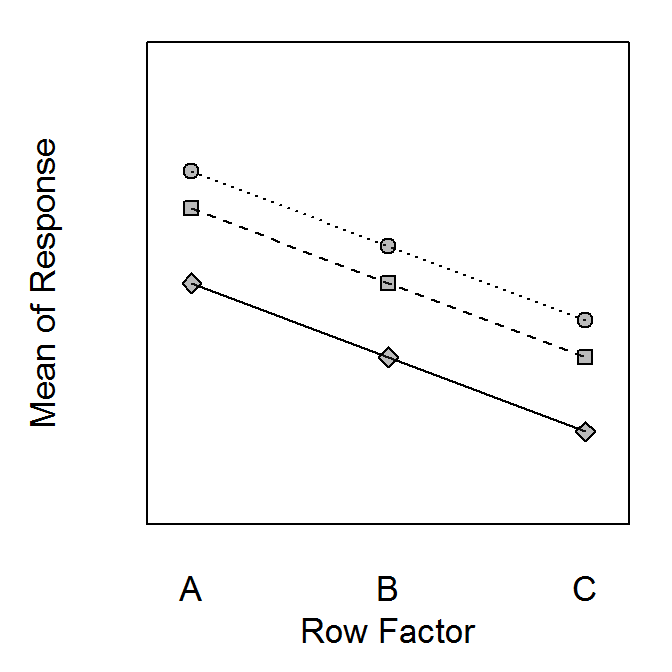
\includegraphics[width=4.5in]{Figs/TWAHW1-1.pdf}}
        \item \raisebox{-.5\height}{\hspace{24pt}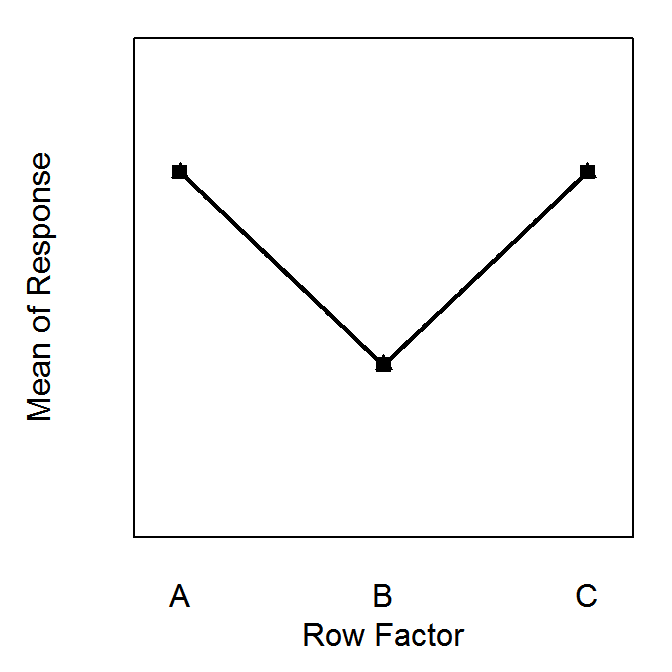
\includegraphics[width=4.5in]{Figs/TWAHW2-1.pdf}}
        \item \raisebox{-.5\height}{\hspace{24pt}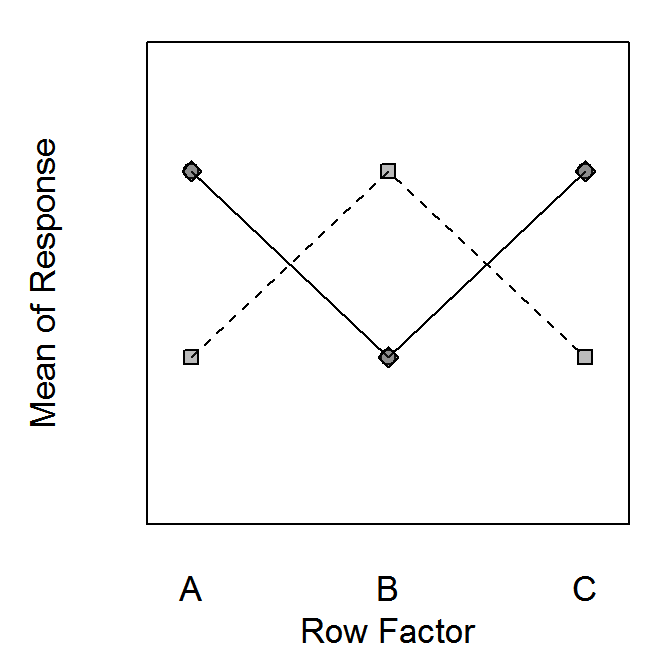
\includegraphics[width=4.5in]{Figs/TWAHW3-1.pdf}}
      \end{Enumerate}

\clearpage
  \item \label{hwprob:LMANOVA22} \textbf{[15 pts]} An experiment was conducted at a large university to determine whether two different instructional methods for teaching a beginning statistics course would yield different levels of achievement.  One instructional method involved using a self-instructional format, including a sequence of slide-tape presentations.  The other method utilized the standard lecture format.  The 100 students who registered for the course were randomly assigned to one of four sections, 25 per section, corresponding to the combinations of one of the two methods with one of two instructors (A and B).  The summarized results from identical final exams in the four sections are

    \begin{Verbatim}
        Variable   Treatment     N       Mean     Median      StDev
        Score      LectA        25      75.45      75.15      14.76
                   LectB        25      74.46      74.48      13.25
                   SelfA        25      83.98      79.97      13.59
                   SelfB        25      80.70      79.15      14.20
    \end{Verbatim}

Use these result to complete the ANOVA table below.  Recreate the table and show your calculations on a separate sheet of paper (R will not help with these calculations).  These answers can be hand-written.

      \begin{center}
        \begin{tabular}{|c|c|c|c|c|c|}
          \hline
          Source & df & SS & MS & F & p \\
          \hline
          \multicolumn{1}{|l|}{Among} &  &  &  &  &  \\
          \hline
          \multicolumn{1}{|l|}{   Instructor} &  &  &  &  &  \\
          \hline
          \multicolumn{1}{|l|}{   Method} &  &  &  &  &  \\
          \hline
          \multicolumn{1}{|l|}{   Instructor*Method} &  &  &  &  &  \\
          \hline
          \multicolumn{1}{|l|}{Within} &  &  &  & \multicolumn{1}{c}{} & \multicolumn{1}{c}{} \\
          \cline{1-4}
          \multicolumn{1}{|l|}{Total} &  & 20227.3 & \multicolumn{1}{c}{} & \multicolumn{1}{c}{} & \multicolumn{1}{c}{} \\
          \cline{1-3}
        \end{tabular}
      \end{center}

\turnpage{200}
  \item \label{hwprob:LMANOVA2Crayfish} \textbf{[15 pts]} \cite{NystromGraneli1997} examined the importance of intraspecific competition for food as a factor regulating survival, growth, and fecundity in noble crayfish (\emph{Astacus astacus}).  In one aspect of their research they examined factors that increased the risk of predation.  In this part of their study, the authors assumed that the number of active crayfish (i.e., not in shelters) was an indicator of the risk of predation (i.e., the crayfish are out of their shelters and are thus more vulnerable).  The authors hypothesized that the risk of predation would be greater if the level of competition was high.  The authors created two levels of competition by regulating how much food the crayfish received (with the assumption being that competition is greater with lesser food).  The two feeding regimes were labeled as FED meaning that the crayfish were fed \emph{ad libitum} and UNFED meaning that they were fed slightly less than a maintenance ration.  In addition, the authors hypothesized that the crayfish would be more active near dusk.  Thus, they also included a time of day factor that had three levels:  1200 (noon), 1700, and 1900.  The authors had a large number of crayfish available to them for this experiment.  They randomly assigned groups of 50 crayfish to each treatment.  After an acclimatization period for the crayfish, the authors recorded the number of crayfish that were active (i.e., not in shelters) in each treatment.  The results of their observations are shown in the data table below.

    \begin{center}
      \begin{tabular}{|c|c|c|c|c|c|c|c|cccccc|}
        \hline
        \widen{-1}{5}{Comp} & Time & \multicolumn{12}{c|}{Number (out of 50) of Active Crayfish} \\
        \hline
        \widen{-1}{5}{Fed} & 1200 & 3 & 2 & 3 & 2 & 2 & 2 &  &  &  &  &  &  \\
        \cline{1-8}
        \widen{-1}{5}{Unfed} & 1200 & 7 & 14 & 4 & 4 & 10 & 5 &  &  &  &  &  &  \\
        \hline
        \widen{-1}{5}{Fed} & 1700 & 4 & 2 & 4 & 3 & 2 & 4 & \multicolumn{1}{c|}{4} & \multicolumn{1}{c|}{3} & \multicolumn{1}{c|}{4} & \multicolumn{1}{c|}{3} & \multicolumn{1}{c|}{4} & 4 \\
        \hline
        \widen{-1}{5}{Unfed} & 1700 & 24 & 33 & 41 & 6 & 22 & 28 & \multicolumn{1}{c|}{12} & \multicolumn{1}{c|}{35} & \multicolumn{1}{c|}{31} & \multicolumn{1}{c|}{30} & \multicolumn{1}{c|}{24} & 39 \\
        \hline
        \widen{-1}{5}{Fed} & 1900 & 3 & 3 & 4 & 2 & 5 & 3 &  &  &  &  &  &  \\
        \cline{1-8}
        \widen{-1}{5}{Unfed} & 1900 & 49 & 13 & 40 & 48 & 47 & 47 &  &  &  &  &  &  \\
        \hline
      \end{tabular}
    \end{center}

    \begin{Enumerate}
      \item Thoroughly check the assumptions for a two-way ANOVA with the original data.  If necessary, transform the data to meet the assumptions of a two-way ANOVA.  If transformed then prove that the assumptions are met on the transformed scale.  [\emph{For simplicity, do not remove any outliers from the data set.  Also, it may not be possible to find a transformation where all assumptions are met.  Thus, try to find the transformation where the critical assumptions are met.  You may check your chosen transformation with me before continuing.}]
      \item Determine if there are significant main effects or an interaction effect with these data.
      \item Thoroughly describe specific differences related to significant main or interaction effects.
      \item Construct a plot or plots that depict the differences identified in the previous question.  Note, this plot should have letters depicting which groups are and are not significantly different.
    \end{Enumerate}

\end{hwsection}



\chapter{Simple Linear Regression}  \label{chap:LMRegression1}
  \vspace{0pt}
    \begin{ChapObj}{\boxwidth}
      \textbf{Chapter Objectives:}
        \begin{Enumerate}
          \item Describe the equation of a line including the meanings of the two parameters.
          \item Describe how the best-fit line to a set of bivariate data is derived.
          \item Understand how to construct hypothesis tests and confidence intervals for parameters and predictions.
          \item Describe the difference between confidence and prediction intervals related to predictions.
          \item Describe the importance of the default hypothesis tests for parameters.
          \item Show all interrelationships among coefficient, ANOVA, and summary computations.
          \item Describe why meeting the assumptions of a regression analysis is important.
          \item Describe what a residual is.
          \item Describe how to assess the four major assumptions of linear regression.
          \item Describe the importance of transforming variables.
          \item Describe three methods for choosing an appropriate variable transformation.
          \item Understand the concept of competing models and their relationship to hypothesis tests in SLR.
          \item Understand how to interpret the results in an ANOVA table.
        \end{Enumerate}
    \end{ChapObj}
  \vspace{-12pt}
\minitoc
\newpage

\lettrine{A}{ simple linear regression (SLR) is used} when a single quantitative response and a single quantitative explanatory variable are considered\footnote{Indicator variable regression (IVR; see \chapref{chap:LMRegression2} is used when multiple explanatory variables are present and some of those are factor variables.  Multiple linear regression (MLR) will be used when multiple quantitative explanatory variables are present.}.  The goals of SLR are to use the value of the explanatory variable to (1) predict future values of the response variable and (2) explain the variability of the response variable.  A simple linear regression, the topic of this chapter, would be used in each of these situations:
\begin{Enumerate}
  \item Predict annual consumption for a species from a biomass estimate.
  \item Evaluate the variability of porcupine body mass based on days since the beginning of winter.
  \item Evaluate the variability in clutch size relative to length of female spiders.
  \item Predict daily energy consumption from the body weight of penguins.
  \item Predict change in duck abundance from the loss of wetlands.
  \item Predict plant shoot dry mass from total leaf length.
\end{Enumerate}

\warn{The two major goals of SLR are to use the explanatory variable to (1) predict a future value of the response variable and (2) explain the variability of the response variable.}

\section{Foundational Review}
\subsection{Variable Definitions}
In SLR, the variable that will be predicted or have its variability explained, is called the \emph{response variable}\footnote{Some call this the \emph{dependant variable}.}.  The other variable, the variable that will be used to make better predictions and to help explain the variability of the response variable, is called the \emph{explanatory variable}\footnote{Some call this the \emph{independent variable}.}.  The explanatory variable is always plotted on the x-axis; thus, the response variable is always plotted on the y-axis.

\defn{Response Variable}{The variable in SLR that is to be predicted or have its variability explained.}

\vspace{-12pt}
\defn{Explanatory Variable}{The variable in SLR that is used to predict or explain the variability of the response variable.}

\subsection{Line Equation}
Both goals of SLR are accomplished by finding the model\footnote{The use of the word ``model'' is used here instead of the word ``line'' because in this class, models other than lines will be fit to some data.  However, all models will be fit by finding a ``scale'' on which the form of the relationship between the response and explanatory variable is linear.} that best fits the relationship between the response variable and the explanatory variable\footnote{It is assumed that you covered the basics of simple linear regression in your introductory statistics course.  Thus, parts of this section will be review, although the nomenclature used may differ somewhat.}.  When examining statistical regression models, the most common expression for the equation of the best-fit line is
\begin{equation}\label{eqn:SLRpopn}
  \mu_{Y|X} = \alpha + \beta_{1}X
\end{equation}
where $Y$ represents the response variable, $X$ the explanatory variable, $\alpha$ the y-intercept and $\beta_{1}$ the slope.  The left-hand-side (LHS) of \eqref{eqn:SLRpopn} is read as ``the mean of Y at a given value of X.''   This terminology is used for the LHS because the best-fit line actually models the mean values of $Y$ at each value of $X$ rather than the individuals themselves.  The model in \eqref{eqn:SLRpopn} is for the population\footnote{This was likely obvious as you noticed the use of Greek letters which are reserved for parameters.}.  The equation of the best-fit line based on the information in the sample is written as
\begin{equation}\label{eqn:SLRsample}
  \hat{\mu}_{Y|X} = \hat{\alpha} + \hat{\beta}_{1}X
\end{equation}
In other words, \eqref{eqn:SLRpopn} is essentially a parameter (i.e., it represents the population line) and \eqref{eqn:SLRsample} is a statistic (i.e., it estimates a parameter based only on the information in a sample).  Thus,  $\alpha$ and $\beta_{1}$ represent the population y-intercept and slope, respectively; whereas $\hat{\alpha}$ and $\hat{\beta}_{1}$ represent the sample y-intercept and slope.

\subsection{Best-Fit Line}
The statistics $(\hat{\alpha}, \hat{\beta}_{1})$ in \eqref{eqn:SLRsample} are determined by finding the values for $(\alpha, \beta_{1})$ that minimize the residual sum-of-squares (RSS).  A residual is the difference between an observed value of the response variable for an individual, $y_{i}$, and a predicted value of the response variable based on the model \eqref{eqn:SLRpopn} given that individuals value of the explanatory variable, $x_{i}$ \figrefp{fig:SLRResidDemo}.  In other words, a residual is computed as $y_{i}-\hat{\mu}_{Y|X=x_{i}}$.

\begin{knitrout}
\definecolor{shadecolor}{rgb}{0.922, 0.922, 0.922}\color{fgcolor}\begin{figure}[h]

{\centering 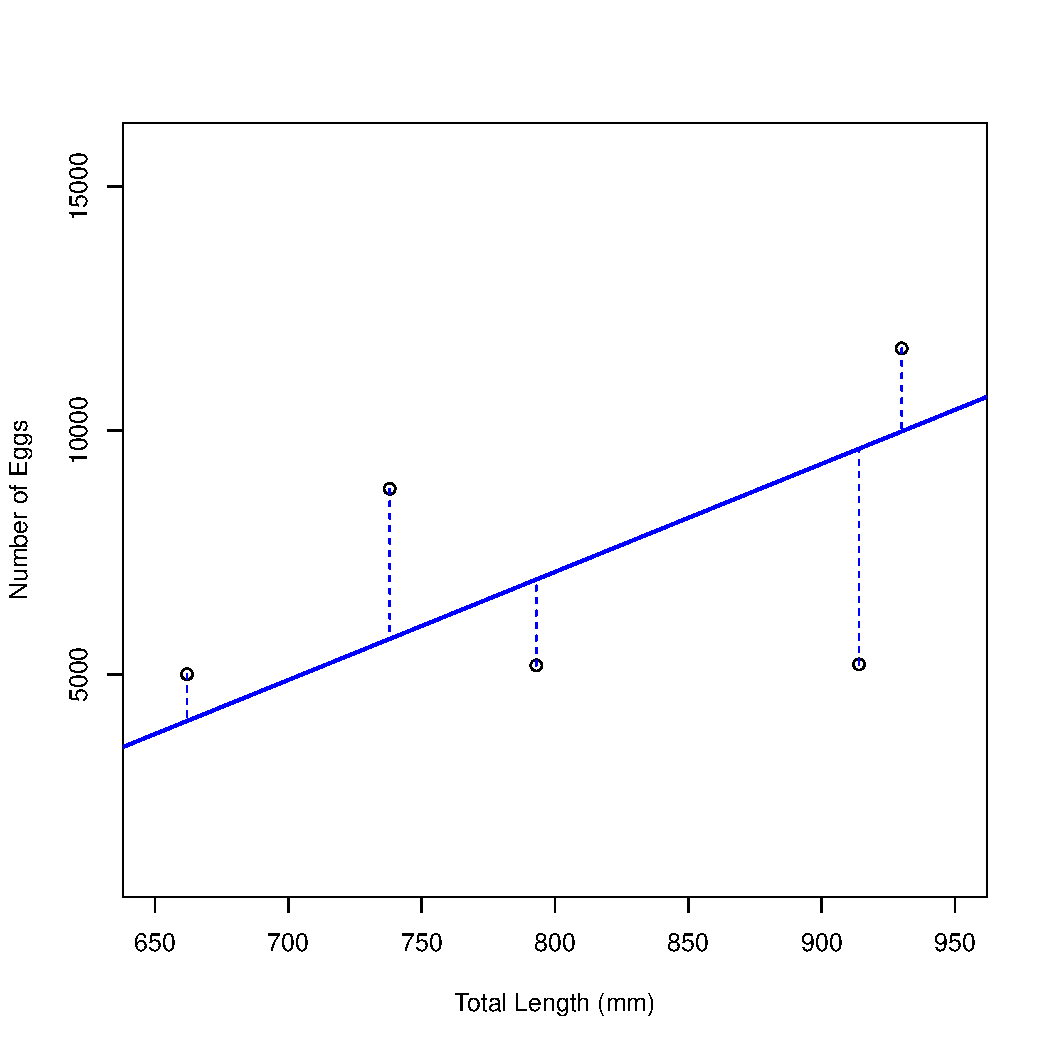
\includegraphics[width=.4\linewidth]{Figs/SLRResidDemo-1} 

}

\caption[Scatterplot with best-fit line illustrating five residuals]{Scatterplot with best-fit line illustrating five residuals.}\label{fig:SLRResidDemo}
\end{figure}


\end{knitrout}

\defn{Residual}{The difference between the observed value of the response variable for an individual and the predicted value of the response variable using the best-fit line; i.e., $y_{i}-\hat{\mu}_{Y|X=x_{i}}$.}

The RSS is the sum of the squares of these residuals, or
\[ RSS = \Sum_{i=1}^{n}\left(y_{i}-\hat{\mu}_{Y|X=x_{i}}\right)^{2} \]
It can be shown with calculus that the RSS is minimized with a slope given by
\[ \hat{\beta}_{1} = r\frac{s_{Y}}{s_{X}} \]
and a y-intercept given by
\begin{equation}\label{eqn:SLRintercept}
    \hat{\alpha} = \overline{Y} - \hat{\beta}_{1}\overline{X}
\end{equation}

where $r$ is the sample correlation coefficient, $\overline{Y}$ and $\overline{X}$ are the sample means, and $s_{Y}$ and $s_{X}$ are the sample standard deviations of the response and explanatory variable, respectively.

\defn{RSS}{Residual Sum-of-Squares}

\vspace{-12pt}
\warn{The best-fit line is the line of all possible lines that minimizes the RSS.}

\subsection{Best-Fit Line in R}
\subsubsection*{Coefficient Results}
The best-fit regression line is obtained with \R{lm()}.  The formula argument to this function is of the form \R{response}$\sim$\R{explanatory}.  As usual, the results of this function should be assigned to an object that can be sent to other functions to extract specific results.  For example, the simple linear regression for predicting the number of eggs based on the total length of a Lake Superior female lake trout is obtained with

\begin{knitrout}
\definecolor{shadecolor}{rgb}{0.922, 0.922, 0.922}\color{fgcolor}\begin{kframe}
\begin{verbatim}
> LT <- read.csv("data/LakeTroutEggs.csv")
> ( lt.lm <- lm(eggs~tl,data=LT) )
Coefficients:
(Intercept)           tl  
  -10620.52        22.15  
\end{verbatim}
\end{kframe}
\end{knitrout}

These results show that the slope of the best-fit line is 22.2 and the intercept is -10620.5.  Thus, with this model, it is predicted that the number of eggs will increase by about 22.2, on average, for each 1 mm increase in total length of a female lake trout.  Because these data are not longitudinal this result is best stated for a 1 mm difference in total length of two female lake trout; i.e., a female lake trout that is 1 mm longer than another female lake trout will have an average of 22.2 more eggs.

\subsubsection*{Fitted-Line Plot}
A visual representation of the best-fit line is obtained by super-imposing the best-fit line onto a scatterplot of the data.  This plot is called a fitted-line plot and can be obtained with \R{fitPlot()} in essentially the same way it was used in previous chapters.  The fitted-line plot for the lake trout egg data \figrefp{fig:SLRLTFittedLinePlot} is obtained with

\begin{knitrout}
\definecolor{shadecolor}{rgb}{0.922, 0.922, 0.922}\color{fgcolor}\begin{kframe}
\begin{verbatim}
>  fitPlot(lt.lm,ylab="Number of eggs",xlab="Total Length",main="")
\end{verbatim}
\end{kframe}\begin{figure}[h]

{\centering \includegraphics[width=.4\linewidth]{Figs/SLRLTFittedLinePlot-1} 

}

\caption[Scatterplot of number of eggs versus total length for Lake Superior lake trout with best-fit line superimposed]{Scatterplot of number of eggs versus total length for Lake Superior lake trout with best-fit line superimposed.}\label{fig:SLRLTFittedLinePlot}
\end{figure}


\end{knitrout}


\section{Inferences} \label{sect:SLRInferences}
\subsection{Slope \& Intercept}
It is very common to make inferences about $\alpha$ and $\beta_{1}$ from the corresponding statistics.  Just like every other statistic, these statistics are subject to sampling variability and, thus, have sampling distributions.  The sampling distributions of $\hat{\alpha}$ and $\hat{\beta}_{1}$ are normally distributed (if the assumptions of SLR are met; see \sectref{sect:SLRAssumptions}) and unbiased\footnote{It is important to think back to your introductory statistics course to remind yourself what it means for a statistic to be unbiased.}.  The standard error of the sample y-intercept is given by
\[ SE_{\hat{\alpha}} = \sqrt{s^{2}_{Y|X}\left(\frac{1}{n}+\frac{\bar{X}^{2}}{(n-1)s_{X}^{2}}\right)} \]
and the standard error of the sample slope is given by
\[ SE_{\hat{\beta}_{1}} = \sqrt{\frac{s^{2}_{Y|X}}{(n-1)s_{X}^{2}}}  \]
where $s^{2}_{Y|X}$ is the variance that measures the natural variability of individuals around the line\footnote{The best-fit line does not perfectly represent every individual.  This statistic is a measure of how the individuals scatter around the line.}.

\warn{The sample slope and sample y-intercept are statistics and thus have sampling distributions and standard errors.}

More complete results from fitting the SLR model to the lake trout egg data are shown in  \tabref{tab:SLRLTResults1}.  All results for the y-intercept are in the row labeled with ``(Intercept).''  All results for the slope are in the row labeled with the variable name of the explanatory variable (\var{tl} in this example).  The estimated y-intercept and slope values are in the column labeled ``Estimate.''  The standard errors for the sample y-intercept and slope are in the column labeled ``Std. Error.''

\begin{table}[h]
  \centering
  \caption{Least-squares regression results for the model $\mu_{eggs|tl} = \alpha + \beta_{1}tl$}\label{tab:SLRLTResults1}
\begin{knitrout}
\definecolor{shadecolor}{rgb}{1, 1, 1}\color{fgcolor}\begin{kframe}
\begin{verbatim}
              Estimate Std. Error t value Pr(>|t|)
(Intercept) -10620.525   1787.520  -5.941 4.22e-08
tl              22.155      2.346   9.442 1.81e-15
---
Residual standard error: 1795 on 99 degrees of freedom
Multiple R-squared: 0.4738,	Adjusted R-squared: 0.4685 
F-statistic: 89.15 on 1 and 99 DF,  p-value: 1.806e-15 
\end{verbatim}
\end{kframe}
\end{knitrout}
\end{table}

Two common hypothesis tests in SLR are to determine whether or not the population y-intercept or the population slope is equal to a particular value.  These hypotheses are written in the typical format as
\[ \begin{split}
H_{A}&: \alpha \neq \alpha_{0} \\
H_{A}&: \beta_{1} \neq \beta_{10}
\end{split} \]
where $\alpha_{0}$ and $\beta_{10}$ represents a specific value for $\alpha$ and $\beta_{1}$.  As an example\footnote{It is assumed that you are familiar with the following test statistic and confidence interval formula from the 1-sample t-test taught in your introductory statistics course.}, the hypothesis for the slope is tested with the following test statistic
\begin{equation}\label{eqn:tTestStat}
  t = \frac{\hat{\beta}_{1}-\beta_{10}}{SE_{\hat{\beta}_{1}}}
\end{equation}
with $df=n-2$.  Familiarly, a confidence interval is constructed with
\[ \hat{\beta}_{1} \pm t^{*}SE_{\hat{\beta}_{1}} \]
The test statistic and confidence interval for the intercept test is constructed similarly.

\warn{Hypothesis tests and confidence intervals for the population slope and population y-intercept are performed with the same general formulas for t- test statistics and confidence intervals learned in your introductory statistics course.  The major difference being that $df=n-2$.}

As an example, suppose that interest is in determining whether or not a significant portion of the variability in the number of eggs in mature female lake trout can be explained by the total length of the fish.  This question translates into a hypothesis to determine if the response and explanatory variable are significantly related.  This in turn translates into a simple hypothesis test to determine if the population slope is equal to zero or not\footnote{You should convince yourself that a test of whether or not the slope is equal to zero, is also a test of whether or not the response and explanatory variable are significantly related}.  Thus, the statistical hypotheses to be tested are
\[ \begin{split}
H_{0}&: \beta_{1} = 0 \\
H_{A}&: \beta_{1} \neq 0
\end{split} \]

The test statistic\footnote{The values used in this test statistic come from \tabref{tab:SLRLTResults1}.} for testing this hypothesis is $t=\frac{22.15-0}{2.35}=9.44$.  Thus, with $df=99$, the p-value is exceptionally small and the null hypothesis is soundly rejected resulting in a conclusion that the number of eggs per female is, in fact, significantly related to the length of the female lake trout.  This conclusion can be made stronger by computing a 95\% confidence interval for the population slope in orer to give an estimate of the direction and magnitude of the relationship.  A 95\% confidence interval for the slope is $22.15\pm1.984*2.35$ or $(17.50, 26.81)$.  Thus, one is 95\% confident that the true change in the mean number of eggs with a one mm increase in total length is between 17.50 and 26.81.

A careful examination of \tabref{tab:SLRLTResults1} shows that the test statistic and p-value for this hypothesis test have already been calculated by R\footnote{As an example, for the population slope, compare the results in the slope row from \tabref{tab:SLRLTResults1} with the results in the previous paragraph.}.  In fact, these t- and p-values are for testing the very common specific hypotheses of whether the model parameter equals zero or not; e.g., tests if the population slope is different from zero.

It is important for you to note that the t- and p-values printed in this output are only useful for testing the particular hypotheses that the corresponding parameter is equal to zero; all other hypothesis tests are NOT computed automatically by R or other common software packages.  However, it is also important to note that testing that the slope is equal to zero is of great importance in linear regression because it determines whether the explanatory and response variable are significantly related or not.

\warn{The default p-values printed by most software programs are for the specific null hypothesis that the corresponding parameter is equal to zero (vs. that it is not).  Those values cannot be used for any other hypothesis tests.}

\vspace{-12pt}
\warn{The test of whether the population slope equals zero or not is also a test of whether the response and explanatory variable are significantly related.}

\subsubsection{Slope \& Intercept Inferences in R}
The information necessary for computing hypothesis tests about the slope and y-intercept (i.e., the results shown in \tabref{tab:SLRLTResults1}) is obtained by submitting the fitted \R{lm} object to \R{summary()}.  In addition, confidence intervals for each parameter in a linear model can be obtained by submitting the saved \R{lm} object to \R{confint()}.  For example, the confidence intervals for the parameters in the lake trout egg data are obtained with\footnote{Note that the 95\% confidence interval for the population slope is found in the row labeled with the explanatory variable.  Thus, in this example, one is 95\% confident that the population slope is between 17.5 and 26.8.}

\begin{knitrout}
\definecolor{shadecolor}{rgb}{0.922, 0.922, 0.922}\color{fgcolor}\begin{kframe}
\begin{verbatim}
> confint(lt.lm)
                   2.5 %      97.5 %
(Intercept) -14167.35175 -7073.69789
tl              17.49882    26.81051
\end{verbatim}
\end{kframe}
\end{knitrout}

A simultaneous confidence ``region'' for both parameters of an SLR actually forms an elliptical region \figrefp{fig:SLRLTConfEllipse}.  The region shown in \figref{fig:SLRLTConfEllipse} is set to contain the point $(\alpha,\beta_{1})$ with 95\% confidence.  In other words, one is 95\% confident that \emph{both} $\alpha$ and $\beta_{1}$ are simultaneously contained within the elliptical region shown.  Interestingly, projections of the extremes of the ellipse onto the ``Intercept'' (i.e., ``X'') and ``slope'' (i.e., ``Y'') axes form univariate 95\% confidence intervals for the intercept and slope parameters, respectively\footnote{Note how these projections have the same endpoints as the results from \R{confint()}.}.

\begin{knitrout}
\definecolor{shadecolor}{rgb}{0.922, 0.922, 0.922}\color{fgcolor}\begin{figure}[h]

{\centering \includegraphics[width=.4\linewidth]{Figs/SLRLTConfEllipse-1} 

}

\caption[Confidence ellipse for ]{Confidence ellipse for $\alpha$ and $\beta_{1}$ from the regression of number of eggs versus total length for Lake Superior lake trout.}\label{fig:SLRLTConfEllipse}
\end{figure}


\end{knitrout}
\vspace{9pt}
Another interesting result illustrated with \figref{fig:SLRLTConfEllipse} is that the regression parameters are highly correlated.  In this instance, as the intercept increases the slope decreases.  Not all regression parameters are highly correlated, but many are.  This may cause some difficulty in some situations; corrections will be addressed when those topics are discussed in subsequent sections.

The testing of hypotheses comparing the slope and intercept to values other than zero can be efficiently computed with \R{hoCoef()}\footnote{This function is a very simple function that computes the test statistic as defined in \eqref{eqn:tTestStat} and then computes the p-value from the t-distribution with the \R{pt()} function.}.  This function requires the saved \R{lm} object as its first argument, a number representing the term in the model to be tested (in SLR \R{term=1} is the intercept and \R{term=2} is the slope) as its second argument, and the null hypothesized value (i.e., $\alpha_{0}$ or $\beta_{10}$) as the third argument.  In addition, the direction of the alternative hypothesis can be defined with the \R{alt=} argument.  For example, the following code can be used to test whether the true slope is greater than 20 eggs (i.e.,  $H_{A}: \beta_{1}>20$),

\begin{knitrout}
\definecolor{shadecolor}{rgb}{0.922, 0.922, 0.922}\color{fgcolor}\begin{kframe}
\begin{verbatim}
> hoCoef(lt.lm,2,20,alt="greater")
 term Ho Value Estimate Std. Error         T df   p value
    2       20 22.15467    2.34644 0.9182716 99 0.1803542
\end{verbatim}
\end{kframe}
\end{knitrout}
Thus, there is very little evidence ($p=0.1804$) that the increase in number of eggs for a 1 mm increase in length is significantly greater than 20\footnote{This is not a surprising result given the confidence interval for the slope computed above.}.


\subsection{Centering \& Intercept} \label{sect:SLRCentering}
Most hypothesis tests in SLR are related to the slope.  However, in some instances, interest may be in the intercept.  However, the interpretation of the y-intercept is often nonsensical because $X=0$ is not within the domain of the explanatory variable.  In other words, the value of the response variable when the explanatory variable is zero is often an extrapolation and can result in exceptionally odd statements.  This problem is further exacerbated when considering inferences about the y-intercept because, as will be shown in the next section, the variability around the model increases as the distance away from the mean of the explanatory variable increases.  Thus, if $X=0$ is considerably outside the range of the data and is, thus, considerably ``away from'' $\bar{x}$ then the variability at the intercept will be very large and statistical power will be very low.

One method for constructing an intercept term that is meaningful is to re-center the explanatory variable to zero.  Variables are re-centered to zero by subtracting the mean of that variable from every observed value of that variable.  In other words, the new variable, $X^{*}$, is formed with $X-\bar{x}$.

Centering the explanatory variable does nothing more than shift the entire distribution from being centered on $\bar{x}$ to being centered on $0$ \figrefp{fig:SLRCentering}.  The interpretation of the y-intercept changes with this shift from representing the average value of $Y$ when $X=0$ to representing the average value of $Y$ when $X=\bar{x}$.  Thus, the $\hat{\alpha}$ from the centered data is likely different than $\hat{\alpha}$ from the original un-centered data.  However, the slope and its interpretation is unchanged as are all predictions\footnote{The researcher must remember to center the value of $X$ though before using the model to predict the mean value of $Y$.}.

\begin{knitrout}
\definecolor{shadecolor}{rgb}{0.922, 0.922, 0.922}\color{fgcolor}\begin{figure}[h]

{\centering \includegraphics[width=.4\linewidth]{Figs/SLRCentering-1} 
\includegraphics[width=.4\linewidth]{Figs/SLRCentering-2} 

}

\caption[Scatterplot of number of eggs versus total length (Left) and centered total length (Right)]{Scatterplot of number of eggs versus total length (Left) and centered total length (Right). The vertical gray line on the left is the mean total length whereas the vertical gray line on the right is at 0 and is the mean centered total length.}\label{fig:SLRCentering}
\end{figure}


\end{knitrout}

As an example, the linear regression of number of eggs in female lake trout on total length and centered total length is shown in Tables \ref{tab:SLRLTResults1} and \ref{tab:SLRLTResults2}, respectively.  Note that the estimated intercept terms in each model are dramatically different as is their corresponding standard errors.  The intercept term from the un-centered model represents the mean number of eggs in a lake trout with a total length of 0.  In contrast, the intercept term from the centered model represents the mean number of eggs in a lake trout with an average total length.  Further notice that all other results are exactly the same between the two models.

\begin{table}[h]
  \centering
  \caption{Least-squares regression results for the model $\mu_{eggs|tl} = \alpha + \beta_{1}(tl-\overline{tl})$}\label{tab:SLRLTResults2}
\begin{knitrout}
\definecolor{shadecolor}{rgb}{1, 1, 1}\color{fgcolor}\begin{kframe}
\begin{verbatim}
            Estimate Std. Error t value Pr(>|t|)
(Intercept) 6172.495    178.568  34.567  < 2e-16
c.tl          22.155      2.346   9.442 1.81e-15
---
Residual standard error: 1795 on 99 degrees of freedom
Multiple R-squared: 0.4738,	Adjusted R-squared: 0.4685 
F-statistic: 89.15 on 1 and 99 DF,  p-value: 1.806e-15 
\end{verbatim}
\end{kframe}
\end{knitrout}
\end{table}

In general, in SLR, centering of the explanatory variable is not critical unless the interpretation of the intercept term is of great importance.  However, a side effect of centering the explanatory variable is that the estimated slope and intercept are then orthogonal -- which, for all practical purposes, means uncorrelated \figrefp{fig:SLRLTConfEllipse2}.  This characteristic allows the centering of explanatory variables to have other uses and positive impacts in multiple linear regressions.

\begin{knitrout}
\definecolor{shadecolor}{rgb}{0.922, 0.922, 0.922}\color{fgcolor}\begin{figure}[h]

{\centering \includegraphics[width=.4\linewidth]{Figs/SLRLTConfEllipse2-1} 

}

\caption[Confidence ellipse for ]{Confidence ellipse for $\alpha$ and $\beta_{1}$ from the regression of number of eggs versus CENTERED total length for Lake Superior lake trout.}\label{fig:SLRLTConfEllipse2}
\end{figure}


\end{knitrout}

\subsubsection*{Centering Variables in R}
A variable is centered in R by subtracting the mean value from the vector of all measurements of the explanatory variable.  The mean of all measurements in a vector is computed with \R{mean()}.  For example, the centered total length of lake trout in the lake trout eggs example is obtained from the original \var{tl} variable with

\begin{knitrout}
\definecolor{shadecolor}{rgb}{0.922, 0.922, 0.922}\color{fgcolor}\begin{kframe}
\begin{verbatim}
> LT$ctl <- LT$tl - mean(LT$tl)
\end{verbatim}
\end{kframe}
\end{knitrout}

This new variable can then be used in \R{lm()} to perform a regression using the centered explanatory variable.

\subsection{Predicting Mean \& Individuals}
One of the major goals of linear regression is to use the best-fit line and a known value of the explanatory variable to predict a future value of the response variable.  This prediction is easily made by plugging the known value of the explanatory variable (generically labeled as $x_{0}$) into the equation of the best-fit line for $X$.  Generically, this is
\[ \hat{\mu}_{Y|X=x_{0}} = \hat{\alpha} + \hat{\beta}_{1}x_{0} \]

For example, the predicted number of eggs for a 700-mm female lake trout is computed by plugging 700 into $\hat{\mu}_{eggs|tl=700}$=-10620.52+22.15*700 = 4887.74 or 4888 eggs.

This prediction is the best guess at the \textbf{mean} number of eggs for all 700-mm individuals and is, thus, also the best guess at the number of eggs for a 700-mm long individual.  So, in essence, this one calculation accomplishes two things: (1) predicts the \textbf{mean} value of the response variable for \textbf{all} individuals with a given value of the explanatory variable and (2) predicts the value of the response variable for \textbf{an} individual with a given value of the explanatory variable.  To keep these two items separate, the first objective (predict the mean) is often called finding a \emph{fitted value} because the best-fit line actually ``fits'' the mean values of $Y$ at a given value of $X$.  The second objective (predict the individual) is often called finding a \emph{predicted value} because ``predictions'' are generally made for individuals.

\defn{Fitted value}{The predicted mean value of the response variable for all individuals with a given value of the explanatory variable.}

\vspace{-12pt}
\defn{Predicted value}{The predicted value of the response variable for an individual with a given value of the explanatory variable.}

Both calculations -- of the fitted value and the predicted value -- are statistics that are subject to sampling variability.  Thus, both results have sampling distributions that are normally distributed\footnote{If the regression assumptions are met; see \sectref{sect:SLRAssumptions}.)} with a mean equal to $\hat{\mu}_{Y|X=x_{0}}$.  The standard error for the fitted value is labeled as $SE_{fits}$ and is given by
\begin{equation}\label{eqn:SLRSEfits}
    \sqrt{s_{Y|X}^{2}\left(\frac{1}{n}+\frac{\left(x_{0}-\bar{X}\right)^{2}}{(n-1)s_{x}^{2}}\right)}
\end{equation}
The standard error for the predicted value is labeled as $SE_{pred}$ and is given by
\begin{equation}\label{eqn:SLRSEpred}
    \sqrt{s_{Y|X}^{2}+s_{Y|X}^{2}\left(\frac{1}{n}+\frac{\left(x_{0}-\bar{X}\right)^{2}}{(n-1)s_{x}^{2}}\right)}
\end{equation}
Both standard errors can be used to construct intervals.  For example, the interval of $\hat{\mu}_{Y|X=x_{0}}\pm t^{*}SE_{fits}$ gives a confidence interval for the mean value of $Y$ when $X$ is equal to $x_{0}$; whereas the interval of $\hat{\mu}_{Y|X=x_{0}}\pm t^{*}SE_{pred}$ gives a prediction interval for the value of $Y$ when $X$ is equal to $x_{0}$.

\warn{A confidence interval is for the mean value of the response variable at a given value of the explanatory variable.  A prediction interval is for the value of the response variable at a given value of the explanatory variable.}

The width of these intervals depends on the value of $x_{0}$.  The $SE_{fit}$ and $SE_{pred}$ are minimized when $x_{0}=\bar{X}$ because $\left(x_{0}-\bar{X}\right)^{2}$ is minimized when $x_{0}=\bar{X}$.  Thus, these intervals are narrowest at $\bar{X}$ and progressively wider as $x_{0}$ is further away from $\bar{X}$\footnote{Make sure you can see why this is true by looking at \eqref{eqn:SLRSEfits} and \eqref{eqn:SLRSEpred}}.  This widening is intuitive because the bulk of the data (or information) is near the ``middle'' of the range of the explanatory variable; thus, confidence in predictions is greatest near the middle and is less near the margins of the range of the explanatory variable.

\warn{Both confidence and prediction intervals are narrowest at the mean of the explanatory variable and get wider further from the mean of the explanatory variable.}

It is critically important to understand the interpretational difference between intervals made using $SE_{fits}$ and those using $SE_{pred}$.  Intervals using $SE_{fits}$ are constructed in conjunction with estimates of the mean value of $Y$ at a given value of $X$.  Thus, $SE_{fits}$ is simply a measure of sampling variability or a measure of how different the mean value of $Y$ at a given $X$ would be if different samples were taken.  In contrast, intervals using $SE_{pred}$ are used in conjunction with estimates of the value of $Y$ at a given value of $X$ for an individual.  Thus, $SE_{pred}$ contains two types of variability; (1) sampling variability associated with estimating the mean and (2) natural variability associated with individuals.  In other words, there is variability associated with estimating the means (as measured by $SE_{fits}$) and there is natural variability among individuals (as measured by $s_{Y|X}^{2}$).  Graphically, sampling variability is illustrated in \figref{fig:SLRConfBands}.  Thus, the dashed lines in \figref{fig:SLRConfBands} illustrate ``confidence bands'' for the mean value of $Y$ at all given values of $X$.  To make ``prediction bands'' that will contain the predicted value of $Y$ for an individual at each given value of $X$, additional natural variability would need to be added onto the ends of each of the confidence bands in \figref{fig:SLRConfBands}.  This additional variability is illustrated by the dashed blue lines in \figref{fig:SLRPredBands} and is also evident by noting the extra $s_{Y|X}^{2}$ when comparing equations \eqref{eqn:SLRSEfits} and \eqref{eqn:SLRSEpred}.

\begin{figure}[h]
  \centering
  \includegraphics[width=3in]{FigsStatic/SLR_Conf_Bands.jpg}
  \caption{Idealistic conceptualization of a best-fit line surrounded by confidence intervals for $\mu_{Y|X}$.}\label{fig:SLRConfBands}
\end{figure}

\begin{figure}[h]
  \centering
  \includegraphics[width=3in]{FigsStatic/SLR_Pred_Bands.jpg}
  \caption{Idealistic conceptualization of a best-fit line surrounded by confidence intervals for $\mu_{Y|X}$ (in red) and prediction intervals for $Y$ (in blue).}\label{fig:SLRPredBands}
\end{figure}

\warn{$SE_{fits}$ represents one type of error - sampling variability related to predicting the mean value of the response variable at a given value of the explanatory variable.  $SE_{pred}$ represents two types of error - sampling variability related to predicting the mean value of the response variable and natural variability related to predicting an individual's difference from that mean.}



For example, suppose that one wants to predict the mean number of eggs for all 700-mm female lake trout (i.e., ``fitted value'').  This requires the calculation of a confidence interval using $SE_{fits}$ because it is related to a \emph{mean} for \emph{all} 700-mm lake trout.  Thus, the mean number of eggs for all 700-mm female lake trout is between 4442 and 5333 \tabrefp{tab:SLRLTPredict}.  Further suppose that one wants to predict the number of eggs for a 700-mm female lake trout (i.e., ``predicted value'').  This requires a prediction interval using $SE_{pred}$ because it is about \emph{an individual} 700-mm lake trout.  Thus, the number of eggs predicted for a 700-mm female lake trout is between 1299 and 8476 \tabrefp{tab:SLRLTPredict}.

\begin{table}[h]
  \centering
  \caption{Fitted values, confidence intervals (top row), and prediction intervals (bottom row) for number of eggs for 700-mm female lake trout.}\label{tab:SLRLTPredict}
\begin{knitrout}
\definecolor{shadecolor}{rgb}{1, 1, 1}\color{fgcolor}\begin{kframe}
\begin{verbatim}
      fit      lwr      upr
 4887.744 4442.281 5333.206
 4887.744 1299.143 8476.345
\end{verbatim}
\end{kframe}
\end{knitrout}
\end{table}

\subsubsection*{Predictions in R}
Future means and individuals can be predicted using the results of a simple linear regression with \R{predict()}.  This function requires three arguments in the following order,
\begin{Itemize}
  \item An \R{lm} object.
  \item A data frame that consists of values of the explanatory variable at which to make predictions.
  \item A string in the \R{interval=} argument that indicates whether to construct a confidence (\R{interval="confidence"}) or prediction (\R{interval="prediction"}) interval.
\end{Itemize}
For example, the confidence interval for the mean number of eggs in all 700-mm total length lake trout is obtained with

\begin{knitrout}
\definecolor{shadecolor}{rgb}{0.922, 0.922, 0.922}\color{fgcolor}\begin{kframe}
\begin{verbatim}
> predict(lt.lm,data.frame(tl=700),interval="confidence")
       fit      lwr      upr
1 4887.744 4442.281 5333.206
\end{verbatim}
\end{kframe}
\end{knitrout}

As another example, prediction intervals for the number of eggs in a 700-mm and in a 770-mm lake trout are obtained with

\begin{knitrout}
\definecolor{shadecolor}{rgb}{0.922, 0.922, 0.922}\color{fgcolor}\begin{kframe}
\begin{verbatim}
> predict(lt.lm,data.frame(tl=c(700,770)),interval="prediction")
       fit      lwr       upr
1 4887.744 1299.143  8476.345
2 6438.570 2859.704 10017.437
\end{verbatim}
\end{kframe}
\end{knitrout}

The most difficult aspect of making predictions in R appears to be the use of the data frame in the second argument of \R{predict()}.  The main thing to remember is that within \R{data.frame()} the name of the explanatory variable must be used exactly as it appeared in the saved \R{lm} object.  In other words, if \var{tl} was used to fit the linear model, then \var{tl} must be used in \R{data.frame()} within \R{predict()}.

The confidence and prediction bands can be plotted by adding the \R{interval=} argument to \R{fitPlot()}.  The \R{interval=} argument can be set to \R{"confidence"} to construct a confidence band, to \R{"prediction"} to construct a prediction band, or \R{"both"} to construct both confidence and prediction bands.  The 95\% confidence and prediction bands are added to the fitted-line plot for the lake trout data \figrefp{fig:SLRLTFittedLinePlot2} with

\begin{knitrout}
\definecolor{shadecolor}{rgb}{0.922, 0.922, 0.922}\color{fgcolor}\begin{kframe}
\begin{verbatim}
> fitPlot(lt.lm,interval="both",xlab="Total Length",ylab="Number of Eggs",main="")
\end{verbatim}
\end{kframe}\begin{figure}[h]

{\centering \includegraphics[width=.4\linewidth]{Figs/SLRLTFittedLinePlot2-1} 

}

\caption[Scatterplot of number of eggs versus total length for Lake Superior lake trout with best-fit line and 95\% confidence and prediction bands superimposed]{Scatterplot of number of eggs versus total length for Lake Superior lake trout with best-fit line and 95\% confidence and prediction bands superimposed.}\label{fig:SLRLTFittedLinePlot2}
\end{figure}


\end{knitrout}

Finally, a visual of the predictions with intervals superimposed on to a fitted-line plot with the confidence and prediction bands can be constructed with \R{predictionPlot()}.  This function takes the exact same arguments as \R{predict()} and returns the predicted values, with intervals, and a visual plot.  For example, the predicted values for 700 and 770 mm lake trout are obtained with

\begin{knitrout}
\definecolor{shadecolor}{rgb}{0.922, 0.922, 0.922}\color{fgcolor}\begin{kframe}
\begin{verbatim}
> predictionPlot(lt.lm,data.frame(tl=c(700,770)),interval="prediction",
  xlab="Total Length",ylab="Number of Eggs",main="")
  obs  tl      fit      lwr       upr
1   1 700 4887.744 1299.143  8476.345
2   2 770 6438.570 2859.704 10017.437
\end{verbatim}
\end{kframe}\begin{figure}[h]

{\centering \includegraphics[width=.4\linewidth]{Figs/SLRLTFittedLinePlot3-1} 

}

\caption[Scatterplot of number of eggs versus total length for Lake Superior lake trout with best-fit line, 95\% confidence and prediction bands superimposed, and 95\% prediction intervals shown for a 700 (interval 1) and 710 (interval 2) mm lake trout]{Scatterplot of number of eggs versus total length for Lake Superior lake trout with best-fit line, 95\% confidence and prediction bands superimposed, and 95\% prediction intervals shown for a 700 (interval 1) and 710 (interval 2) mm lake trout.}\label{fig:SLRLTFittedLinePlot3}
\end{figure}


\end{knitrout}

and visualized in \figref{fig:SLRLTFittedLinePlot3}.  Inasmuch as the results of \R{predict()} are included in \R{predictionPlot()}, it is suggested that you use \R{predictionPlot()} to make predictions as this should help you avoid making extrapolations with the model.

\subsection{Models \& SS}
As with all linear models (see \chapref{chap:LMFoundations}), the important hypothesis tests of SLR can be reduced to the method of comparing two models' lack-of-fit to the data.  From above it was seen that the hypothesis test to determine if the response and explanatory variable are significantly related is

\[ \begin{split}
H_{0}&: \beta_{1} = 0 \\
H_{A}&: \beta_{1} \neq 0
\end{split} \]

This can be written in terms of models as

\[ \begin{split}
H_{0}&: \mu_{Y|X} = \alpha \\
H_{A}&: \mu_{Y|X} = \alpha + \beta_{1}X
\end{split} \]

Furthermore, by substituting \eqref{eqn:SLRintercept} into \eqref{eqn:SLRsample}, the sample best-fit line can be rewritten as follows

\[ \begin{split} \hat{\mu}_{Y|X} &= \overline{Y} - \hat{\beta}_{1}\overline{X} + \hat{\beta}_{1}X \\
                                 &= \overline{Y} + \hat{\beta}_{1}\left(X-\overline{X}\right) \end{split} \]

Thus, if $\hat{\beta}_{1}=0$ then the model reduces to $\hat{\mu}_{Y|X}=\overline{Y}$.

Therefore, testing the hypothesis that the slope is equal to zero is equivalent to testing whether the very simple model of $\overline{Y}$ (or, equivalently, the constant $\hat{\alpha}$) adequately fits the data versus a more complicated model where a slope is needed \figrefp{fig:SLRModelsVisual}.  Said another way, this is the same as testing whether the mean value of $Y$ is the same for all $X$s (i.e., no slope, no relationship) or whether the mean value of $Y$ depends on the value of $X$ (i.e., a slope, there is a relationship).

\begin{knitrout}
\definecolor{shadecolor}{rgb}{0.922, 0.922, 0.922}\color{fgcolor}\begin{figure}[h]

{\centering \includegraphics[width=.4\linewidth]{Figs/SLRModelsVisual-1} 
\includegraphics[width=.4\linewidth]{Figs/SLRModelsVisual-2} 

}

\caption[Scatterplot illustrating two competing models for describing the relationship between number of eggs and total length]{Scatterplot illustrating two competing models for describing the relationship between number of eggs and total length.  The horizontal red line is placed at the mean number of eggs and represents the simple model (Left).  The blue line is the best-fit line and represents the full model (Right).}\label{fig:SLRModelsVisual}
\end{figure}


\end{knitrout}

\warn{The simple model in SLR represents a flat line at the mean of the response variable.  The full model in SLR represents a line with a significant slope.}

Of course, the lack-of-fit of the two models is calculated by summing the squared residuals using predictions from the two models.  Specifically, the lack-of-fit of the simple model is computed with residuals using predictions from the mean value of the response variable (\figref{fig:SLRModelsResids}-Left), or

\begin{equation}\label{eqn:SLRsimpleRSS}
  SS_{Total} = \Sum_{i=1}^{n}\left(y_{i}-\overline{Y}\right)^{2}
\end{equation}

As expected, this SS is called $SS_{Total}$ because it is the basis of the measure of the ``total'' variability in the response variable as calculated by the variability around the overall mean.

The lack-of-fit of the full model is computed with residuals using predictions from the best-fit regression line (\figref{fig:SLRModelsResids}-Right), or

\[ SS_{Residual} = \Sum_{i=1}^{n}\left(y_{i}-\hat{\mu}_{Y|X}\right)^{2} = \Sum_{i=1}^{n}\left(y_{i}-\left(\hat{\alpha}+\hat{\beta}_{1}x_{i}\right)\right)^{2} \]

This SS is termed $SS_{Residual}$ in SLR, but it is exactly analogous to $SS_{Within}$ from Chapters \ref{chap:LMFoundations} and \ref{chap:LMANOVA1}.

\begin{knitrout}
\definecolor{shadecolor}{rgb}{0.922, 0.922, 0.922}\color{fgcolor}\begin{figure}[h]

{\centering \includegraphics[width=.4\linewidth]{Figs/SLRModelsResids-1} 
\includegraphics[width=.4\linewidth]{Figs/SLRModelsResids-2} 

}

\caption[Scatterplots illustrating two competing models for describing the relationship between number of eggs and total length]{Scatterplots illustrating two competing models for describing the relationship between number of eggs and total length.  The horizontal red line is placed at the mean number of eggs and represents the simple model (Left).  The blue line is the best-fit line and represents the full model (Right).  Residuals for each model are shown on the respective graphs.}\label{fig:SLRModelsResids}
\end{figure}


\end{knitrout}

\warn{The $SS_{Total}$ measures the ``variability'' in the simplest model, which is just the mean of the response variable.  Thus, $SS_{Total}$ measures the maximum total ``variability'' in the response variable.}

As always, the $SS_{Total}$ can be partitioned into two parts; generically as

\[ SS_{Total} = SS_{Residual} + SS_{Regression} \]

and more specifically as

\[ \Sum_{i=1}^{n}\left(y_{i}-\overline{Y}\right)^{2} = \Sum_{i=1}^{n}\left(y_{i}-\hat{\mu}_{Y|X}\right)^{2} + \Sum_{i=1}^{n}\left(\hat{\mu}_{Y|X}-\overline{Y}\right)^{2} \]

$SS_{Residual}$ represents the part of the total variability in the response variable that is not explained by the full model.  The difference between $SS_{Total}$ and  $SS_{Residual}$ is called  $SS_{Regression}$ and represents the part of the total variability in the response variable that \emph{is} explained by the full model.  This part is exactly analogous to $SS_{Among}$ from Chapters \ref{chap:LMFoundations} and \ref{chap:LMANOVA1}, but is called $SS_{Regression}$ in SLR because it is the amount of variability explained by using the best-fit regression line.  Thus, as would be expected, $SS_{Regression}$ measures how much ``better'' the full model fits compared to the simple model.  However, as with $SS_{Among}$, this statistic must be converted to an $MS$ and then, ultimately, to an F test statistic.

\warn{$SS_{Total} = SS_{Residual} + SS_{Regression}$.}

\vspace{-12pt}
\warn{The residual SS ($SS_{Residual}$) is the measure of the ``variability'' in the response variable that is unexplained when an explanatory variable is incorporated into the model.}

\vspace{-12pt}
\warn{The regression SS ($SS_{Regression}$) is the measure of the ``variability'' in the response variable that is explained when an explanatory variable is incorporated into the model.}


\subsubsection{ANOVA Table}
The three $SS$ just discussed are converted to $MS$ by dividing by their respective $df$.  The $df_{Total}=n-1$ as discussed in \chapref{chap:LMFoundations}.  The $df_{Residual}$ is equal to the number of individuals minus the number of parameters in the full model\footnote{This is a general rule for the calculation of $df_{Residual}$.} -- i.e., $n-2$.  Thus, using the rule that dfs partition in the same way as $SS$, the $df_{Regression}$ is $(n-1)-$$(n-2)$$=1$\footnote{It is also common that the $df_{Regression}$ is the difference in number of parameters between the full and simple models.}.

\warn{The regression df are always 1 in SLR.}

With these definitions of $df$, the $MS$ are computed as such,

\begin{equation}\label{eqn:SLRsimpleMS}
  MS_{Total} = \frac{SS_{Total}}{df_{Total}} = \frac{\Sum_{i=1}^{n}\left(y_{i}-\overline{Y}\right)^{2}}{n-1} = s_{Y}^{2}
\end{equation}
\begin{equation}\label{eqn:SLRfullMS}
  MS_{Residual} = \frac{SS_{Residual}}{df_{Residual}} = \frac{\Sum_{i=1}^{n}\left(y_{i}-\hat{\mu}_{Y|X}\right)^{2}}{n-2} = s_{Y|X}^{2}
\end{equation}
\[ MS_{Regression} = \frac{SS_{Regression}}{df_{Regression}} = \frac{\Sum_{i=1}^{n}\left(\hat{\mu}_{Y|X}-\overline{Y}\right)^{2}}{1} \]

The F test statistic is computed in a manner very similar to what was described in \chapref{chap:LMFoundations}.  Specifically,
\[ F = \frac{MS_{Regression}}{MS_{Residual}} \]
with $df_{Regression}$ numerator and $df_{Residual}$ denominator df.

As usual, the degrees-of-freedom ($df$), sum-of-squares ($SS$), mean-squares ($MS$), F test statistic ($F$), and corresponding p-value are summarized in an analysis of variance table \tabrefp{tab:SLRLTANOVA}.

\begin{table}[h]
  \centering
  \caption{Analysis of variance table for the regression of $\mu_{eggs|tl} = \alpha + \beta_{1}tl$.}\label{tab:SLRLTANOVA}
\begin{knitrout}
\definecolor{shadecolor}{rgb}{1, 1, 1}\color{fgcolor}\begin{kframe}
\begin{verbatim}
           Df    Sum Sq   Mean Sq F value    Pr(>F)
tl          1 287104252 287104252  89.148 1.806e-15
Residuals  99 318832897   3220534                  
Total     100 605937149                            
\end{verbatim}
\end{kframe}
\end{knitrout}
\end{table}


The results in \tabref{tab:SLRLTANOVA} indicate that there is a significant relationship between \var{eggs} and \var{tl} ($p<0.00005$).  This same result indicates that a full model with a slope term on the \var{tl} variable is significantly ``better'' at fitting the observed data then a simple model that does not contain a slope term.

In addition to the primary objective of comparing the full and simple models, several items of interest can be identified from an analysis of variance table.  Using \tabref{tab:SLRLTANOVA} as an example, the following items are identified:
\begin{Itemize}
  \item The variance of individuals about the regression line ($s_{Y|X}^{2}$) is given by $MS_{Residual}$ (e.g., =3220534).
  \item The variance of individuals about the mean ($s_{Y}^{2}$) is given by $MS_{Total}$ (e.g., $SS_{Total}$=287104252+318832897 divided by $df_{Total}$=1+99 or 6059371.5).
  \item The F test statistic is equal to the square\footnote{This is a general rule between the T and F distributions.  An F with $1$ numerator df and $\nu$ denominator df is equal to the square of a T with $\nu$ df.} of the t test statistic from testing $H_{0}:\beta_{1}=0$.
\end{Itemize}

\subsubsection*{Regression ANOVA Table in R}
The ANOVA table for a SLR is obtained by submitting the saved \R{lm} object to \R{anova()} (e.g., the ANOVA table results for the lake trout egg data shown in \tabref{tab:SLRLTANOVA} were obtained with \R{anova(lt.lm)}).

\subsubsection{Coefficient Of Determination}
The coefficient of determination ($R^{2}$) is a measure of the proportion of the total variability in the response variable that is explained by knowing the value of the explanatory variable\footnote{It is assumed that you learned this statistic in your introductory statistics course.}.  Thus, from the $SS$ definitions above,

\[ R^{2} = \frac{SS_{Regression}}{SS_{Total}} \]

In essence, $R^{2}$ is a measure of the strength for predictions that can be made.  In other words, $R^{2}$ values near one indicate a relationship that is very strong and will lead to precise predictions, whereas $R^{2}$ values near zero indicate a very weak relationship with correspondingly weak predictions.

\subsubsection*{Coefficient of Determination in R}
The coefficient of determination is shown in the output following ``multiple R-squared`` when a saved \R{lm} object is submitted to the \R{summary()} function.  An example is shown in \tabref{tab:SLRLTResults2}.  This value can also be isolated by submitting the saved \R{lm} object to \R{rSquared()}.


\section{Assumptions} \label{sect:SLRAssumptions}
Simple linear regression has five major assumptions,
\begin{Enumerate}
  \item Each individual is independent of each and every other individual (``independence'' assumption).
  \item The mean values of $Y$ at each given value of $X$ fall on a straight line (``linearity'' assumption).
  \item The variances of $Y$ at each given value of $X$ are all equal (to $\sigma^{2}_{Y|X}$) (``homoscedasticity'' assumption).
  \item The values of $Y$ at each given value of $X$ are normally distributed (``normality'' assumption).
  \item No outliers.
\end{Enumerate}
These five assumptions lead to the idealistic model illustrated in \figref{fig:SLRIdealModel}.



\begin{knitrout}
\definecolor{shadecolor}{rgb}{0.922, 0.922, 0.922}\color{fgcolor}\begin{figure}[h]

{\centering \includegraphics[width=.4\linewidth]{Figs/SLRIdealModel-1} 
\includegraphics[width=.4\linewidth]{Figs/SLRIdealModel-2} 

}

\caption[Two depictions of the assumptions of the simple linear regression model]{Two depictions of the assumptions of the simple linear regression model.  The blue ``best-fit'' line intersects the mean of each normal distribution.  Each normal distribution represents the distribution of the response variable for all individuals at a particular value of the explanatory variable.  Example data are shown by the black dots.}\label{fig:SLRIdealModel}
\end{figure}


\end{knitrout}
\vspace{9pt}
It is important to note that the first assumption states that the \textbf{means} all fall on a straight line, not that the individuals do.  This is why the left-hand-sides of equations \eqref{eqn:SLRpopn} and \eqref{eqn:SLRsample} contain $\mu_{Y|X}$ rather than just $Y$.  This is also demonstrated by the observation that the line drawn on \figref{fig:SLRIdealModel} intersects the means of the individual normal distributions.  Thus, don't lose track of the fact that \eqref{eqn:SLRpopn} represents the mean values of the response variable at a given value of the explanatory variable and not the individual values of the response variable.

The model in \eqref{eqn:SLRpopn} can be modified to represent each individual (rather than the mean of individuals) by adding an error term ($\epsilon$).  Thus, the model to represent individuals is written
\begin{equation}\label{eqn:SLRpopnErr}
  Y|X = \alpha + \beta_{1}X + \epsilon
\end{equation}
From the assumptions (as illustrated in \figref{fig:SLRIdealModel}), the errors will be normally distributed with a mean of 0 (because the line passes through the $\mu_{Y|X}$ and the residuals, or errors, are computed from that point) and a variance of $\sigma^{2}_{Y|X}$.  Thus, in shorthand, the $\epsilon\sim N(0,\sigma_{Y|X}$).

\warn{The errors about the best-fit line are $N(0,\sigma_{Y|X}$).}

The $\sigma^{2}_{Y|X}$ is called ``the common variance about the model'' and represents the natural variability about the model (i.e., ``how much does each individual naturally vary from the model'').  This common variance is exactly analogous to $MS_{Within}$ discussed in Chapters \ref{chap:LMFoundations} and \ref{chap:LMANOVA1} and is the basis of nearly all inferences in SLR (as seen in \sectref{sect:SLRInferences}).  The common variance is a parameter that is estimated using the residuals from the individuals in a sample with

\[ s^{2}_{Y|X} = MS_{Residual} = \frac{\Sum_{i=1}^{n}\left(y_{i}-\hat{\mu}_{Y|X=x_{i}}\right)^{2}}{n-2} \]

Thus, $\sigma^{2}_{Y|X}$ is a population variance and $s^{2}_{Y|X}$ is a sample variance.

\subsection{Diagnostics}
The assumption of the independence of individuals is generally assessed with common sense and is controlled through proper sample design just as was described in Chapters \ref{chap:LMFoundations}-\ref{chap:LMANOVA2}\footnote{If the individuals are ordered by time or space then the Durbin-Watson statistic can be used to determine if the individuals are serially correlated or not.  Generally, the $H_{0}:$ ``not serially correlated'' and $H_{A}:$ ``is serially correlated'' are the hypotheses for the Durbin-Watson test.  Thus, p-values $<\alpha$ result in the rejection of $H_{0}$ and the conclusion of a lack of independence.  In this case, the regression assumption would be violated and other methods, primarily time-series methods, should be considered.}.

The linearity assumption is the most important assumption in SLR; i.e., the form of the bivariate relationship must be linear in order to fit a line to it.  Problems with the linearity assumption are diagnosed by close examination of the fitted-line plot.  In some instances, the departures from linearity may be subtle or the strength of relationship so strong and the range of the explanatory variable so large that departures from linearity are difficult to discern.  In these instances, one should look at a residual plot from the model fit.  The residual plot effectively ``zooms in'' on the best-fit line such that subtle departures from linearity can be more easily identified.  The most common departures from linearity look like parabolas, but more ``complicated'' structures may also be noted \figrefp{fig:SLRResidPlotViolations}.

\begin{knitrout}
\definecolor{shadecolor}{rgb}{0.922, 0.922, 0.922}\color{fgcolor}\begin{figure}[h]

{\centering \includegraphics[width=.8\linewidth]{Figs/SLRResidPlotViolations-1} 

}

\caption[Residual plots illustrating when the regression assumptions are met (upper-left) and three common assumption violations]{Residual plots illustrating when the regression assumptions are met (upper-left) and three common assumption violations.}\label{fig:SLRResidPlotViolations}
\end{figure}


\end{knitrout}

\warn{The linearity assumption can be addressed with a fitted-line or a residual plot.}

\vspace{-12pt}
\warn{A fitted-line or residual plot that exhibits no obvious curvature is evidence that the linearity assumption has been met.}

The homoscedasticity assumption is also vital because all inferences in SLR depend on $s^{2}_{Y|X}$.  The homoscedasticity assumption assures that the variability is constant around the line and that $s^{2}_{Y|X}$ estimates a constant quantity.  If this assumption is not met, then a common variance does not exist, $s^{2}_{Y|X}$ measures a quantity that does not exist, and all of the SE calculations from \sectref{sect:SLRInferences} will not work properly.  Difficulties with the homoscedasticity assumption are diagnosed by close examination of a residual plot.  If the points on the residual plot show the same degree of scatter from left-to-right then the homoscedasticity assumption is likely met.  A common violation of the assumption appears as a funnel shape from left-to-right \figrefp{fig:SLRResidPlotViolations}.

\warn{The homoscedasticity assumption is most often addressed with a residual plot.}

\vspace{-12pt}
\warn{A residual plot that exhibits no vertical compression of points is evidence that the homoscedasticity assumption has been met.}

Interpreting residual plots requires some practice and experience.  The trick to examining residual plots is to look for distinctive patterns and shapes.  Most novice statisticians find too much detail in residual plots, identifying every subtle curvature and change in variability.  If distinct patterns do not exist then the assumptions are probably adequately met.  Remember, a residual plot with random scatter and no discernible pattern is an indication that the linearity and homoscedasticity assumptions have been met.

The normality assumption is dealt with exactly as it was in Chapters \ref{chap:LMFoundations}-\ref{chap:LMANOVA2}.  It is virtually impossible in most SLR to test the normality of residuals at each given value of $X$ because there typically is very few replicates of each value of $X$.  Thus, the assumption is assessed with the Anderson-Darling normality test of the residuals from the full model.

The assumption of no outliers is also tested exactly as described in Chapters \ref{chap:LMFoundations}-\ref{chap:LMANOVA2}; i.e., with a hypothesis test using the Studentized residuals and a Bonferroni correction.  However, further discussion of outliers in SLR is warranted.  \cite{Fox1997} describes ``unusual'' observations the best with,

\begin{quote}
Unusual data are problematic in linear models fit by least squares because they can unduly influence the results of the analysis, and because their presence may signal that the model fails to capture important characteristics of the data.
\end{quote}

In its simplest sense, a regression outlier is an individual for which the response variable is unusual given the value of the explanatory variable and the overall ``fit'' of the model.  Following the arguments of \cite{Fox1997}, regression outliers are shown in \figref{fig:SLRDiagnosticsConcept}-left and \figref{fig:SLRDiagnosticsConcept}-middle.  In contrast, a univariate outlier is an individual for which the value of a variable is unusual relative to the mean of that single variable.  An outlier for the response variable and for the explanatory variable, but not a regression outlier is shown in \figref{fig:SLRDiagnosticsConcept}-right.  Note that in \figref{fig:SLRDiagnosticsConcept}-right that the outlying individual is ``extreme'' along both the x- and y-axes but not relative to the linear model fit.  Univariate outliers are not necessarily regression outliers.  However, sometimes the two types of outliers are found in the same individual -- e.g., \figref{fig:SLRDiagnosticsConcept}-middle.

\begin{knitrout}
\definecolor{shadecolor}{rgb}{0.922, 0.922, 0.922}\color{fgcolor}\begin{figure}[h]

{\centering \includegraphics[width=.95\linewidth]{Figs/SLRDiagnosticsConcept-1} 

}

\caption[Illustration of the concepts of outliers and influence in a simple linear regression]{Illustration of the concepts of outliers and influence in a simple linear regression.  Each plot consists of one SLR fit to the ``original'' data (i.e., black solid line and black dots) and another SLR fit to the ``original'' data with the addition of one ``unusual'' point (point shown by red ``x'' and fitted line shown by red dashed line).}\label{fig:SLRDiagnosticsConcept}
\end{figure}


\end{knitrout}
\vspace{9pt}
Individuals that substantially impact the fitted line (i.e., result in substantially different values for the regression coefficients; \figref{fig:SLRDiagnosticsConcept}-middle) are called \emph{influential points}.  The ``influence'' of an individual is related to both it's horizontal distance from the center of the explanatory variable and its vertical distance from the best-fit line.  Intuitively then, highly influential points are points that have a combined ``large'' distance from left-to-right and top-to-bottom relative to the best-fit line.  It is possible that a highly influential point will not appear as an outlier in \R{outlierTest()} because of the high influence it has on the position of the line.  Thus, influential points are diagnosed with careful attention to the fitted-line and residual plots.

\defn{Influential Point}{An individual whose inclusion in the data set substantially impacts the coefficients of the fitted line.}

\subsubsection*{Assumption Checking in R}
The fitted-line plot, residual plot, Anderson-Darling normality test, and the outlier test are constructed exactly as described\footnote{That is, by using \R{fitPlot()}, \R{residPlot()}, \R{adTest()}, and \R{outlierTest()}.} in Chapters \ref{chap:LMFoundations}-\ref{chap:LMANOVA2}.  The residual plot, however, plots the residuals versus the fitted values from the full model rather than a boxplot of residuals versus level names.


\section{Transformations} \label{sect:SLRTransformations}
If one or more of the linearity, homoscedasticity, normality, or outlier assumptions are violated then the data may be transformed to a different scale where the assumptions are met.  Either the response or explanatory variable can be transformed, although transformation of the response variable is generally more effective.  In general, the family of power transformations (see \sectref{sect:AOVTransformations}) will be considered for both the response and explanatory variables, although some special transformations can be used in specific situations (e.g., $\sin^{-1}\sqrt{Y}$ for proportions or percentage data).

\warn{If the normality, linearity, or homoscedasticity assumption is violated then a transformation of variables should be considered.}

\subsection{Selecting Power Transformations}
Power transformations for the variables in a SLR can be selected from a variety of methods -- (1) based on theory, (2) from past experience, or (3) trial-and-error with dynamic graphics.  Specifics of these methods are discussed in the following sections.

\subsubsection*{Theoretical Transformations}
Transformations may be chosen if a theoretical functional form for the relationship between the response and explanatory variables can be identified.  For example, many relationships follow a non-linear power function -- $Y=aX^{b}$ -- where $X$ and $Y$ are variables (as always) and $a$ and $b$ are scalars (i.e., constant numbers).  An example of this type of data is shown in \figref{fig:SLRPowerFun1}.

\begin{knitrout}
\definecolor{shadecolor}{rgb}{0.922, 0.922, 0.922}\color{fgcolor}\begin{figure}[h]

{\centering \includegraphics[width=.4\linewidth]{Figs/SLRPowerFun1-1} 
\includegraphics[width=.4\linewidth]{Figs/SLRPowerFun1-2} 

}

\caption[Fitted line plot (Left) and residual plot (Right) for data simulated from a power function, ]{Fitted line plot (Left) and residual plot (Right) for data simulated from a power function, $Y=aX^{b}$. The residual plot is overlaid with a LOESS smoother function (red line) to highlight the curvature.}\label{fig:SLRPowerFun1}
\end{figure}


\end{knitrout}

If logarithms are taken of both sides of a power function then the form reduces to

\[ \begin{split}
  log(Y) &= log(aX^{b}) \\
  log(Y) &= log(a) + log(X^{b}) \\
  log(Y) &= log(a) + blog(X)
\end{split} \]

which, because $log(Y)$ and $log(X)$ are still variables and $log(a)$ is still a constant, is in a linear form.  Thus, transforming both the response and explanatory variable to the logarithm scale will ``linearize'' a relationship that is known to theoretically follow a power function (\figref{fig:SLRPowerFun2}; note the lack of curvature in both plots).

\begin{knitrout}
\definecolor{shadecolor}{rgb}{0.922, 0.922, 0.922}\color{fgcolor}\begin{figure}[h]

{\centering \includegraphics[width=.4\linewidth]{Figs/SLRPowerFun2-1} 
\includegraphics[width=.4\linewidth]{Figs/SLRPowerFun2-2} 

}

\caption[log-log transform of power function]{Scatterplot (Left) and residual plot (Right) from a log-log transformation of the data simulated from power function and shown in \figref{fig:SLRPowerFun1}.}\label{fig:SLRPowerFun2}
\end{figure}


\end{knitrout}
\vspace{9pt}
Another common form is the non-linear exponential form -- $Y=ae^{bX}$ -- where $e$ is the base of the natural log and is a constant.  An example of this type of data is shown in \figref{fig:SLRExponentialFun1}.  Again, taking the natural log of both sides reduces this functional form to

\[ \begin{split}
  log(Y) &= log(ae^{bX}) \\
  log(Y) &= log(a) + log(e^{bX}) \\
  log(Y) &= log(a) + bX
\end{split} \]

Thus, transforming the response, but not the explanatory, variable to the logarithm scale will ``linearize'' a relationship that is known to theoretically follow an exponential function \figrefp{fig:SLRExponentialFun2}.

\begin{knitrout}
\definecolor{shadecolor}{rgb}{0.922, 0.922, 0.922}\color{fgcolor}\begin{figure}[h]

{\centering \includegraphics[width=.4\linewidth]{Figs/SLRExponentialFun1-1} 
\includegraphics[width=.4\linewidth]{Figs/SLRExponentialFun1-2} 

}

\caption[Scatterplot (Left) and residual plot (Right) for data simulated from an exponential function, ]{Scatterplot (Left) and residual plot (Right) for data simulated from an exponential function, $Y=ae^{bX}$.  The residual plot is overlaid with a LOESS smoother function (red line) to highlight the curvature.}\label{fig:SLRExponentialFun1}
\end{figure}


\end{knitrout}

\begin{knitrout}
\definecolor{shadecolor}{rgb}{0.922, 0.922, 0.922}\color{fgcolor}\begin{figure}[h]

{\centering \includegraphics[width=.4\linewidth]{Figs/SLRExponentialFun2-1} 
\includegraphics[width=.4\linewidth]{Figs/SLRExponentialFun2-2} 

}

\caption[log-transformed exponential function.]{Scatterplot (Left) and residual plot (Right) for log-transformed data simulated from an exponential function and shown in \figref{fig:SLRExponentialFun1}.}\label{fig:SLRExponentialFun2}
\end{figure}


\end{knitrout}

Other common equation types, their transformations to a linear form, and estimates of the model parameters are shown in \tabref{tab:SLRTransformForms}.  Many of these models are important in specific scientific fields.

\begin{sidewaystable}
  \centering
  \caption{Common mathematical models, their transformations to a linear form, and parameter estimates..}\label{tab:SLRTransformForms}
\begin{tabular}{|l|c|c|}
\multicolumn{1}{l}{} & \multicolumn{2}{c}{Model Forms} \\
\cline{1-3}
\widen{-2}{7}{Model Name} & Standard & Linear \\
\cline{1-3}
\widen{-2}{7}{Exponential} & $Y=ae^{bX}$ & $log(Y)=log(a)+bX$ \\
\cline{1-3}
\widen{-2}{7}{Power Function} & $Y=aX^{b}$ & $log(Y)=log(a)+blog(X)$ \\
\cline{1-3}
\widen{-2}{7}{Modified Power Function} & $Y=aX^{b}+c$ & $log(Y-c)=log(a)+blog(X)$ \\
\cline{1-3}
\widen{-2}{7}{Sigmoid} & $Y=\frac{c}{1+aX^{b}}$ & $log\left(\frac{c}{Y}-1\right)=log(a)+blog(X)$ \\
\cline{1-3}
\widen{-2}{7}{Exponential Sigmoid} & $Y=\frac{c}{1+ae^{bX}}$ & $log\left(\frac{c}{Y}-1\right)=log(a)+bX$ \\
\cline{1-3}
\widen{-2}{7}{Exponential Saturation} & $Y=a\left(1-e^{bX}\right)$ & $log(a-Y)=log(a)+bX$\\
\cline{1-3}
\widen{-2}{7}{Maxima Function} & $Y=aXe^{bX}$ & $log\left(\frac{Y}{X}\right)=log(A)+bX$ \\
\cline{1-3}
\widen{-2}{7}{Modified Inverse} & $Y=\frac{a}{b+X}$ & $\frac{1}{Y}=\frac{b}{a}+\frac{1}{a}X$ \\
\cline{1-3}
\widen{-2}{7}{Hyperbola} & $Y=\frac{aX}{b+X}$ & $\frac{X}{Y}=\frac{b}{a}+\frac{1}{a}X$ \\
\cline{1-3}
\end{tabular}

    \vspace{0.2in}

\begin{tabular}{|l|c|c|c|c|c|c|}
\multicolumn{1}{l}{} & \multicolumn{2}{c}{Transformations} & \multicolumn{1}{c}{} & \multicolumn{3}{c}{Parameter Estimates} \\
\cline{1-3}\cline{5-7}
\widen{-2}{7}{Model Name} & Response & Explanatory &  & a & b & c \\
\cline{1-3}\cline{5-7}
\widen{-2}{7}{Exponential} & $log(Y)$ & $X$ &  & $e^{intercept}$ & $slope$ & -- \\
\cline{1-3}\cline{5-7}
\widen{-2}{7}{Power Function} & $log(Y)$ & $log(X)$ &  &  $e^{intercept}$ & $slope$ & -- \\
\cline{1-3}\cline{5-7}
\widen{-2}{7}{Modified Power Function} & $log(Y-c)$ & $log(X)$ &  & $e^{intercept}$ & $slope$ & estimated \\
\cline{1-3}\cline{5-7}
\widen{-2}{7}{Sigmoid} & $log\left(\frac{c}{Y}-1\right)$ & $log(X)$ &  & $e^{intercept}$ & $slope$ & estimated \\
\cline{1-3}\cline{5-7}
\widen{-2}{7}{Exponential Sigmoid} & $log\left(\frac{c}{Y}-1\right)$ & $X$ &  & $e^{intercept}$ & $slope$ & estimated \\
\cline{1-3}\cline{5-7}
\widen{-2}{7}{Exponential Saturation} & $log(a-Y)$ & $X$ &  & $e^{intercept}$ & $slope$ & -- \\
\cline{1-3}\cline{5-7}
\widen{-2}{7}{Maxima Function} & $log\left(\frac{Y}{X}\right)$ & $X$ &  & $e^{intercept}$ & $slope$ & -- \\\cline{1-3}\cline{5-7}
\widen{-2}{7}{Modified Inverse} & $\frac{1}{Y}$ & $X$ &  & $\frac{1}{slope}$ & $\frac{intercept}{slope}$ & -- \\
\cline{1-3}\cline{5-7}
\widen{-2}{7}{Hyperbola} & $\frac{X}{Y}$ & $X$ &  & $\frac{1}{slope}$ & $\frac{intercept}{slope}$ & -- \\
\cline{1-3}\cline{5-7}
\end{tabular}

\end{sidewaystable}


\subsubsection*{Transformations from Experience}
Finally, transformations for the response variable may be determined based on common transformations for a particular type of data.  Transformations for some common types of data are shown in \tabref{tab:RegCommonTransforms}.

\begin{table}[h]
  \centering
  \caption{Common response transformations and their typical usage.}\label{tab:RegCommonTransforms}
  \begin{tabular}{|p{1.6in}|p{4.4in}|}
    \hline
    \widen{-2}{6}{$Y^{*}=Y^{0.5}$} & Commonly used for discrete count data (comes from Poisson distribution theory). \\
    \hline
    \widen{-2}{6}{$Y^{*}=Y^{0.5}+(Y+1)^{0.5}$} & Same as above except for use when some values are 0 or very small. \\
    \hline
    \widen{-2}{6}{$Y^{*}=ln(Y+1)$} & Use when a logarithm transformation is warranted but there are 0s in the data. \\
    \hline
    \widen{-2}{6}{$Y^{*}=Y^{-1}$} & Often used when a response time is recorded.  This transformation changes the units from the scale of time per response to number of responses per time. \\
    \hline
    \widen{-2}{6}{$Y^{*}=sin^{-1}\left(Y^{0.5}\right)$} & Commonly used when the data recorded are proportions or percentages. \\
    \hline
  \end{tabular}
\end{table}

It should also be noted that \cite{Weisberg1985} suggested that if the ratio of maximum to minimum value for the explanatory variable is greater than 10 then it should be transformed to the natural log scale.

\subsubsection*{Trial-and-Error}
Transformations for the response and explanatory variable can be identified by trying a variety of powers for each variable and exploring the results of each.  Of course, this is a tedious process.  Fortunately, computer programs exist for dynamically determining the effect of transforming each variable.  When using these programs the user should attempt to transform just the response variable first.

\subsection*{Back-Transformation Issues}
As discussed in \sectref{sect:AOVTransformationsInterp}, back-transformation is the process of reversing the results found on the transformed scale to the original scale for ease of interpretation.  In regression analyses, the coefficients and predicted values can be thought of as being one of two types.  The intercept, fitted values, and predicted values (along with the endpoints of their confidence intervals) can be thought of as being estimates of average values.  These values are back-transformed as discussed in \sectref{sect:AOVTransformationsInterp}, including the use of the correction factor when a log transformation is used\footnote{Note, however, that the $MS_{Within}$ is replaced with $MS_{Residual}$ so that the correction factor is $e^{\frac{MS_{Residual}}{2}}$.}.  In contrast, the slope is thought of as being an estimate of a rate of change.  Back-transformation of the slope must be interpreted differently.

The back-transformed values of rates (i.e., slopes) from some transformed scales may have a useful interpretational meaning on the original scale.  For example, the back-transformed slope when the response variable has been transformed to the natural log scale is an estimate of the multiplicative change in the mean value of the response variable for a one unit change of the explanatory variable.  Make a clear note of the word ``multiplicative'' in the previous sentence.  Without transformation, the slope is an estimate of how much is ``added'' to the mean of $Y$ for a unit change in $X$; however, back-transforming the slope from the log scale is an estimate of how much the mean of $Y$ is multiplied by for a unit change of $X$.

This interpretation can be illustrated by first looking at the difference in the log-transformed means for a unit change in $X$,

\[log\left(\mu_{Y|X+1}\right)-log\left(\mu_{Y|X}\right) = \left[\alpha+\beta_{1}(X+1)\right] - \left[\alpha+\beta_{1}X\right] = \beta_{1}\]

Thus, not surprisingly, on the log-transformed scale a unit change in $X$ results in a $\beta_{1}$ unit change in the natural logarithm mean of $Y$.  Now, raise both sides of this equation to the power of $e$ and simplify,

\[ \begin{split}
  e^{\beta_{1}} &= e^{log(\mu_{Y|X+1})-log(\mu_{Y|X})} \\
  e^{\beta_{1}} &= e^{log\left(\frac{\mu_{Y|X+1}}{\mu_{Y|X}}\right)} \\
  e^{\beta_{1}} &= \frac{\mu_{Y|X+1}}{\mu_{Y|X}}
\end{split} \]

Thus, $e^{\beta_{1}}$ does NOT represent the difference in two means, rather it represents the ratio of two means on the original scale.

\warn{The value of a slope back-transformed from a natural log transformation represents the ratio of the two means separated by one unit of the explanatory variable on the original scale.  In other words, this back-transformed values it he multiplicative change in the mean response for a unit change in the explanatory variable.}

Note that the correction factor discussed in \sectref{sect:AOVTransformationsInterp} is NOT used when back-transforming rates.  Also, note that this interpretation on the original scale is only true if a log transformation was used.  Useful interpretations on the original scale can not be found for most other transformations.  Thus, the slope should \emph{NOT} be back-transformed if a transformation other than a logarithm was used.

\warn{Do NOT back-transform slopes if other than a log transformation was used.}

\subsection{Polynomial Regression}
The power transformations discussed above have a tendency to simultaneously ``fix'' violations of the linearity, homoscedasticity, and normality assumptions.  This can be troublesome if only one of these assumptions is violated.  For example, it is possible to have data that meet the normality and homoscedasticity assumptions, but are non-linear.  In this case, a power transformation may linearize the data, but may then also make the residuals non-normal or heteroscedastic.  In this example, the meeting of two assumptions was ``traded for'' the meeting of just one assumption.

In this specific situation -- non-linear data with homoscedastic, normal residuals --  it may be appropriate to fit what is called a polynomial regression.  A polynomial regression consists of a generic model of

\[ \mu_{Y|X}=\alpha+\beta_{1}x +\beta_{2}x^{2}+\beta_{3}x^{3}+\beta_{4}x^{4}+\ldots \]

Generally speaking, the polynomial regression model will have one more term (i.e., highest exponent) than the number of ``turns'' in the data.  So, if the form of the relationship looks like a parabola (i.e., one ``turn'') then a model that stops with $X^{2}$ would be tried.  If the data has two ``turns'' then a model that stops with $X^{3}$ would be tried.  Models with more than three or four terms are rarely used because of their complexity.

An example of this type of data is shown in \figref{fig:SLRPolynomial1}.  Clearly a linear model does not fit these data.  However, the residuals do not show an increasing variance around the loess line shown in the residual plot.  Thus, these data are a good candidate to be fit by a polynomial regression.  In fact, a polynomial regression with three terms seems to fit the data well \figrefp{fig:SLRPolynomial2}.

\begin{knitrout}
\definecolor{shadecolor}{rgb}{0.922, 0.922, 0.922}\color{fgcolor}\begin{figure}[h]

{\centering \includegraphics[width=.4\linewidth]{Figs/SLRPolynomial1-1} 
\includegraphics[width=.4\linewidth]{Figs/SLRPolynomial1-2} 

}

\caption[Fitted line plot (Left) and residual plot (Right) for the fit of a linear model to data simulated from a cubic model]{Fitted line plot (Left) and residual plot (Right) for the fit of a linear model to data simulated from a cubic model.}\label{fig:SLRPolynomial1}
\end{figure}


\end{knitrout}

\begin{knitrout}
\definecolor{shadecolor}{rgb}{0.922, 0.922, 0.922}\color{fgcolor}\begin{figure}[h]

{\centering \includegraphics[width=.4\linewidth]{Figs/SLRPolynomial2-1} 
\includegraphics[width=.4\linewidth]{Figs/SLRPolynomial2-2} 

}

\caption[Fitted line plot (Left) and residual plot (Right) for the fit of ]{Fitted line plot (Left) and residual plot (Right) for the fit of $\mu_{Y|X}=\alpha+\beta_{1}X+\beta_{2}X^{2}+\beta_{3}X^{3}$ to data simulated from a cubic model.}\label{fig:SLRPolynomial2}
\end{figure}


\end{knitrout}

Polynomial regression generally falls under the heading of multiple linear regression and will not be discussed further here.  However, at this point, note that polynomial regression is a useful technique if only the linearity assumption has been violated.

\warn{Polynomial regressions are useful when ONLY the linearity assumption has been violated.  If more than one assumption is violated then polynomial regression is unlikely to solve the problem (and, thus, a power transformation should be considered).}


\subsection{Transformations in R}
The trial-and-error method of finding a transformation uses \R{transChooser()} with the only difference being that a start value for the explanatory value can be included in the \R{startx=} argument and that a slider bar will be provided for both the explanatory and response variables.  Once a transformation has been identified the variable is transformed exactly as described in Chapters \ref{chap:LMFoundations}-\ref{chap:LMANOVA2}.


\section{Example Analyses}
\subsection{Lake Trout Fecundity}
\subsubsection*{Introduction}
\cite{Schram1993} examined the relationship between the total length and the number of eggs found in female lake trout from Lake Superior.  Schram's primary goal was to develop a model that could be used to predict the number of eggs produced by a female lake trout from the total length of that fish.  This relationship could be used in subsequent models used to manage the population of lake trout.

\subsubsection*{Data Collection}
Lake trout were collected during the spawning season from set netting areas in the Apostle Islands, Wisconsin.  A sample of 101 ripe but not spent female lake trout over the range of observed lengths were sacrificed and the eggs removed by dissection.  For each fish, the total length (TL; mm) and weight (g) was recorded and the total number of eggs counted.  The data are stored in \dfile{LakeTroutEggs.csv} (\href{https://github.com/droglenc/NCData/blob/master/LakeTroutEggs.csv}{view}, \href{https://raw.githubusercontent.com/droglenc/NCData/master/LakeTroutEggs.csv}{download}, \href{https://github.com/droglenc/NCData/blob/master/LakeTroutEggs_meta.txt}{meta}).

\subsubsection*{EDA \& Assumption Checking}


The initial fit of the untransformed simple linear regression model of the number of eggs on total length indicated that the linear model was adequate for these data  and the residuals were approximately symmetric \figrefp{fig:SLRLTResidA}.  The residuals were weakly, but not significantly, non-normal (Anderson-Darling $p=0.0595$).  However, the outlier test, as displayed in the residual plot, indicated that observation 96 was a significant outlier.  A closer examination of observation 96 showed that (1) the number of eggs was 31\% larger than the next highest number of eggs for similarly sized fish, (2) the number of eggs was 78\% larger than predicted by the linear model, and (3) five fish were larger but none produced more eggs.  There is no indication that either the length or the number of eggs for this fish were measured in error.  Thus, in an effort to produce a model that represents ``typical'' female lake trout this ``unusual'' observation was removed from further analysis.

\begin{knitrout}
\definecolor{shadecolor}{rgb}{0.922, 0.922, 0.922}\color{fgcolor}\begin{figure}[h]

{\centering \includegraphics[width=.8\linewidth]{Figs/SLRLTResidA-1} 

}

\caption[Residual plot (Left) and histogram of residuals (Right) from the fit of a SLR model to the raw Lake Superior lake trout data]{Residual plot (Left) and histogram of residuals (Right) from the fit of a SLR model to the raw Lake Superior lake trout data.}\label{fig:SLRLTResidA}
\end{figure}


\end{knitrout}



The fit of the untransformed simple linear regression model of the number of eggs on total length, without observation 96, indicated that the linear model still adequately fit the data \figrefp{fig:SLRLTResidB}, the residuals were largely homoscedastic \figrefp{fig:SLRLTResidB} and approximately normal (Anderson-Darling $p=0.1684$), and there were no significant outliers left in these data.  Thus, a simple linear regression, with no transformations, will be fit to the data with observation 96 removed.

\begin{knitrout}
\definecolor{shadecolor}{rgb}{0.922, 0.922, 0.922}\color{fgcolor}\begin{figure}[h]

{\centering \includegraphics[width=.8\linewidth]{Figs/SLRLTResidB-1} 

}

\caption[Residual plot (Left) and histogram of residuals (Right) from the fit of a SLR model to the raw Lake Superior lake trout data with observation 96 removed]{Residual plot (Left) and histogram of residuals (Right) from the fit of a SLR model to the raw Lake Superior lake trout data with observation 96 removed.}\label{fig:SLRLTResidB}
\end{figure}


\end{knitrout}

\subsubsection*{Results}
There is a significant relationship between the number of eggs produced and the total length of female Lake Superior lake trout (ANOVA $p<0.00005$).  The relationship is only moderately strong ($R^{2}=$0.476) and is characterized by the linear equation $\mu_{eggs|tl}=$20.699tl-9588.084 \tabrefp{tab:SLRLTResults3}.  Thus, a 1-mm increase in the total length of a female lake trout corresponds to an average increase of approximately 20.7 eggs with a 95\% prediction interval of between 16.3 and 25.1 eggs.

\begin{table}[h]
  \centering
  \caption{Coefficient results from the fit of eggs produced on total length of the raw Lake Superior lake trout data with observation 96 removed.}\label{tab:SLRLTResults3}
\begin{knitrout}
\definecolor{shadecolor}{rgb}{1, 1, 1}\color{fgcolor}\begin{kframe}
\begin{verbatim}
             Estimate Std. Error t value Pr(>|t|)
(Intercept) -9588.084   1669.328  -5.744 1.04e-07
tl             20.699      2.195   9.431 2.08e-15
---
Residual standard error: 1658 on 98 degrees of freedom
Multiple R-squared: 0.4758,	Adjusted R-squared: 0.4704 
F-statistic: 88.94 on 1 and 98 DF,  p-value: 2.083e-15 
\end{verbatim}
\end{kframe}
\end{knitrout}
\end{table}


As an example, a female lake trout with a total length of 650 mm would be predicted to have 3866 eggs with a 95\% confidence interval of 527 to 7206 eggs.  Examples for fish of other lengths are shown in \tabref{tab:SLRLTResults4}.

\begin{table}[h]
  \centering
  \caption{Predicted number of eggs and 95\% prediction intervals for female Lake Superior lake trout with total lengths of 650, 750, and 850 mm.}\label{tab:SLRLTResults4}
\begin{knitrout}
\definecolor{shadecolor}{rgb}{1, 1, 1}\color{fgcolor}\begin{kframe}
\begin{verbatim}
  tl      fit       lwr       upr
 650 3866.361  527.1333  7205.589
 750 5936.276 2629.4759  9243.076
 850 8006.190 4674.6984 11337.683
\end{verbatim}
\end{kframe}
\end{knitrout}
\end{table}

\subsubsection*{Conclusion}
A significant, but only moderately strong, relationship was found between the number of eggs produced and the total length of ``typical'' female lake trout from Lake Superior.  A model was produced that can be used to predict the number of eggs in female lake trout of different total lengths but, because the fit is only moderately strong, these predictions exhibit substantial variability.  Further, it must be noted that this model was fit with the exclusion of one observed fish that had an ``unusually'' large number of eggs given its total length.  Thus, these results are only appropriate for individuals that don't have an ``unusually'' large number of eggs given their total length.

\subsubsection*{Appendix -- R commands}
\begin{Verbatim}[formatcom=\color{red},xleftmargin=5mm,commandchars=\\\{\}]
> LakeTroutEggs <- read.csv("data/LakeTroutEggs.csv")
> lt.lm1 <- lm(eggs~tl,data=LakeTroutEggs)
> fitPlot(lt.lm1,main="")
> residPlot(lt.lm1)
> adTest(lt.lm1$residuals)
> LakeTroutEggs[tl>870 & tl<880,]        # finding fish with similar length to #96
> (eggs[96]-eggs[94])/eggs[94]
> lt.lm1$residuals[96]/lt.lm1$fitted.values[96]
> rank(tl)[96]; rank(eggs)[96]
> LakeTroutEggs1 <- LakeTroutEggs[-96,]  # remove #96
> lt.lm2 <- lm(eggs~tl,data=LakeTroutEggs1)
> fitPlot(lt.lm2,main="")
> residPlot(lt.lm2)
> adTest(lt.lm2$residuals)
> anova(lt.lm2)
> summary(lt.lm2)
> confint(lt.lm2)
> new <- c(650,750,850)
> predictionPlot(lt.lm2,data.frame(tl=new),interval="prediction")
\end{Verbatim}


\subsection{Fish Consumption Estimation}
\subsubsection*{Introduction}

Fish population consumption is an important process linking predator populations to their prey resources.  Simple tools are needed to enable fisheries managers to estimate population consumption.  One such possible simple tool is to estimate population consumption from estimates of the number or biomass of animals in the population.

\subsubsection*{Data Collection}
\cite{Liaoetal2005} assembled, from the literature, a data set of 74 individual estimates of annual consumption by freshwater fish populations and their mean annual population size, 41 of which also included estimates of mean annual biomass.  The data set included 14 freshwater fish species from 10 different bodies of water.  The authors hoped to develop a simple relationship between population food consumption and the numbers or biomass of fish in the population.  This analysis will focus on the relationship between population consumption and biomass of the population.

\subsubsection*{EDA \& Assumption Checking}


An initial EDA of the data indicates a large amount of variability in both the consumption and biomass variables with outlying individuals in both variables.  In addition, the fitted-line and residual plots indicate a lack of linearity and a broad heteroscedasticity and the Anderson-Darling test indicates a non-normality ($p<0.00005$).  These results all indicate that a transformation should be explored.

\begin{knitrout}
\definecolor{shadecolor}{rgb}{0.922, 0.922, 0.922}\color{fgcolor}\begin{figure}[h]

{\centering \includegraphics[width=.8\linewidth]{Figs/SLRFCPlot1-1} 

}

\caption[Residual plot (Left) and histogram of residuals (Right) for the regression of annual population consumptions on population biomass]{Residual plot (Left) and histogram of residuals (Right) for the regression of annual population consumptions on population biomass.}\label{fig:SLRFCPlot1}
\end{figure}


\end{knitrout}



The natural log of biomass (explanatory variable) was initially used because the ratio of maximum to minimum biomass was 1161795.  A natural log transformation for the food consumption variable was also found through a trial-and-error process using \R{transChooser()}.  The relationship between log(consumption) and log(biomass) was linear (\figref{fig:SLRFCPlot2}-Left).  However, the residual plot indicated a slight heteroscedasticity, though this may be apparent because of the lack of data for smaller and larger values of biomass.  The residuals were non-normal (Anderson-Darling $p=0.0042$) and decidedly right-skewed (\figref{fig:SLRFCPlot2}-Right).  Examination of the residual plot (\figref{fig:SLRFCPlot2}-Middle) indicated that observation 3 was an outlier and, due to its position to the far left, a potentially influential point.  Observation 3 was one of only two measurements made at substantially smaller biomass values then the bulk of the observations.  It is not clear that this observation is in error, nor is it apparent that the observation is ``unusual'' as their is only one comparable value to compare it to.  Observation 3 will remain in the data set, but its effect on the regression results will be commented on in the conclusion.  The linear regression model was fit to the log-log transformed data as the linearity and homoscedasticity assumptions were largely met and no other transformation proved ``better.''

\begin{knitrout}
\definecolor{shadecolor}{rgb}{0.922, 0.922, 0.922}\color{fgcolor}\begin{figure}[h]

{\centering \includegraphics[width=.8\linewidth]{Figs/SLRFCPlot2-1} 

}

\caption[Residual plot (Left) and histogram of residuals (Right) for the regression of natural-log transformed annual population consumption on natural-log transformed population biomass]{Residual plot (Left) and histogram of residuals (Right) for the regression of natural-log transformed annual population consumption on natural-log transformed population biomass.}\label{fig:SLRFCPlot2}
\end{figure}


\end{knitrout}

\subsubsection*{Results}
The relationship between log(consumption) and log(biomass) was significantly positive (ANOVA $p<0.00005$).  In fact, it appears that as the log(biomass) increases by one unit that the average log(consumption) increases by approximately 1.00 \tabrefp{tab:SLRFCCoef} units with a 95\% confidence interval between 0.95 and 1.04 units \tabrefp{tab:SLRFCCoefCI}.  Alternatively, a one unit increase in biomass results in an average 2.59 to 2.83 \textbf{times} increase in annual population consumption.

\begin{table}[h]
  \centering
  \caption{Summary results for the regression of $\mu_{log(consumption)|log(biomass)} = \alpha + \beta_{1}log(biomass)$.}\label{tab:SLRFCCoef}
\begin{knitrout}
\definecolor{shadecolor}{rgb}{1, 1, 1}\color{fgcolor}\begin{kframe}
\begin{verbatim}
            Estimate Std. Error t value Pr(>|t|)
(Intercept)  1.25316    0.21199   5.911 6.88e-07
logbio       0.99615    0.02105  47.334  < 2e-16
---
Residual standard error: 0.4199 on 39 degrees of freedom
  (33 observations deleted due to missingness)
Multiple R-squared: 0.9829,	Adjusted R-squared: 0.9825 
F-statistic:  2241 on 1 and 39 DF,  p-value: < 2.2e-16 
\end{verbatim}
\end{kframe}
\end{knitrout}
\end{table}

\begin{table}[h]
  \centering
  \caption{Confidence intervals for parameters in $\mu_{log(consumption)|log(biomass)} = \alpha + \beta_{1}log(biomass)$.}\label{tab:SLRFCCoefCI}
\begin{knitrout}
\definecolor{shadecolor}{rgb}{1, 1, 1}\color{fgcolor}\begin{kframe}
\begin{verbatim}
                2.5 %   97.5 %
(Intercept) 0.8243679 1.681954
logbio      0.9535799 1.038715
\end{verbatim}
\end{kframe}
\end{knitrout}
\end{table}

As an example, suppose that interest is in predicting the mean population consumption for all systems with a biomass of 20000 kg.  This prediction would be accomplished by first converting the given biomass to log(biomass) and plugging that value into the equation of the best-fit line to predict the log(consumption) \tabrefp{tab:SLRFCPred}.  The predicted value and the end points of the confidence interval would then be used as the powers of $e$ to ``back-transform'' the results to the original scale.  These back-transformed values are $58991$ and $77023$.  However, because the natural log transformation was used for the response variable, these back-transformed values should be corrected for back-transformation bias by multiplying each value by $e^{\frac{s^{2}_{Y|X}}{2}}$$=e^{\frac{0.4199^{2}}{2}}$$=e^{0.088}$$=1.092$\footnote{Note that $s^{2}_{Y|X}$=0.4199 as shown in the ``Residual standard error'' portion of \tabref{tab:SLRFCCoef}}.  With this correction, the mean consumption level for all systems with a biomass of 20000 kg would be expected to be between $64428$ and $84122$ kg.

\begin{table}[h]
  \centering
  \caption{Results for the prediction of the mean log(consumption) for a biomass of 20000 kg.}\label{tab:SLRFCPred}
\begin{knitrout}
\definecolor{shadecolor}{rgb}{1, 1, 1}\color{fgcolor}\begin{kframe}
\begin{verbatim}
     fit      lwr      upr
 11.1185 10.98514 11.25185
\end{verbatim}
\end{kframe}
\end{knitrout}
\end{table}

\subsubsection*{Conclusion}
A significant, and very strong, relationship was found between the natural log annual population consumption and the natural log biomass for fish species from a variety of aquatic ecosystems.  A model was developed from this relationship that can be used to predict the annual population consumption of a system from the measured biomass in the system.

One observation, a system with a possibly unusually high annual population consumption value relative to its very low biomass level, was an apparent outlier and influential point in the development of the model.  This point was not removed from the analysis because it was not obviously in error or unusual.  However, if it had been deleted, the changes in the estimates of the slope, intercept, and predicted mean log(consumption) given a biomass of 20000 kg would have changed very little \tabrefp{tab:SLRFCOutlier}.

\begin{table}[h]
  \centering
  \caption{Confidence intervals for the slope, intercept, and predicted mean log(consumption) for the regression of log annual population consumption on log biomass with and without observation 3.}\label{tab:SLRFCOutlier}
  \begin{Verbatim}[xleftmargin=5mm]
                                     w/ obs 3       w/o obs 3
slope                         ( 0.954, 1.039) ( 0.983, 1.059)
intercept                     ( 0.824, 1.682) ( 0.591, 1.366)
predicted log(consumption)    (10.985,11.252) (10.975,11.203)
  \end{Verbatim}
\end{table}

\vspace{-24pt}
\subsubsection*{Appendix -- R commands}
\vspace{-18pt}
\begin{Verbatim}[formatcom=\color{red},xleftmargin=5mm,commandchars=\\\{\}]
> Consumption <- read.csv("data/Consumption.csv")
> Consumption1 <- Consumption[!is.na(Consumption$biomass),] # removing missing data
> fcb.lm1 <- lm(consumption~biomass,data=Consumption1)
> fitPlot(fcb.lm1,main="",pts=19,ltyp=2)
> residPlot(fcb.lm1)
> adTest(fcb.lm1$residuals)
> transChooser(fcb.lm1)
> Consumption1$logcons <- log(Consumption1$consumption)
> Consumption1$logbio <- log(Consumption1$biomass)
> fcb.lm2 <- lm(logcons~logbio,data=Consumption1)
> fitPlot(fcb.lm2,main="")
> residPlot(fcb.lm2)
> adTest(fcb.lm2$residuals)
> anova(fcb.lm2)
> summary(fcb.lm2)
> confint(fcb.lm2)
> predictionPlot(fcb.lm2,data.frame(logbio=log(20000)),interval="c")
> Consumption2 <- Consumption1[-3,]  # remove individual #3 to assess its impact
> fcb.lm3 <- lm(logcons~logbio,,data=Consumption2)
> fitPlot(fcb.lm3,main="")
> residPlot(fcb.lm3)
> adTest(fcb.lm3$residuals)
> confint(fcb.lm3)
> predictionPlot(fcb.lm3,data.frame(logbio=log(20000)),interval="c")
\end{Verbatim}

\clearpage
\section{Summary Process}
The following is a template for a process of fitting a simple linear regression model.  This template can be used initially to get a feel for how to proceed but should not be considered as a concrete process for all models.

\vspace{-10pt}
\begin{Enumerate}
  \item Perform a thorough EDA.
    \begin{Itemize}
      \item Pay close attention to the form, strength, and outliers on the scatterplot [\R{plot()}] of the response and explanatory variables.
    \end{Itemize}
  \item Fit the untransformed ultimate full model [\R{lm()}].
  \item Check the assumptions of the fit of the model.
    \begin{Itemize}
      \item Check the linearity of the relationship with a fitted-line plot [\R{fitPlot()}] and residual plot [\R{residPlot()}].
      \item Check homoscedasticity with a fitted-line plot and residual plot.
      \item Check normality of residuals with an Anderson-Darling test [\R{adTest()}] and histogram of residuals [\R{residPlot()}].
      \item Check for outliters and influential points with the outlier test [\R{outlierTest()}], fitted-line plot, and residual plot.
    \end{Itemize}
  \item If an assumption or assumptions are violated then attempt to find a transformation where the assumptions are met.
    \begin{Itemize}
      \item Use the trial-and-error method [\R{transChooser()}], theory, or experience to identify possible transformations for the response variable and, possibly, for the explanatory variable.
      \item If only an ``unusual'' or influential observation exists (i.e., linear, homoscedastic, and normal residuals) and no transformation corrects the ``problem'' then consider removing that observation from the data set.
    \end{Itemize}
  \item Fit the ultimate full model with the transformed variable(s) or reduced data set.
  \item Construct an ANOVA table for the full model [\R{anova()}] and interpret the overall F-test.
  \item Summarize findings with coefficient results [\R{summary()}, \R{confint()}] and fitted-line plot [\R{fitPlot()}].
  \item Make predictions if desired [\R{predictionPlot()}].
\end{Enumerate}


\turnpage{100}
\begin{hwsection}{All questions below (except where noted) should be typed, refer to tables of output, be answered with complete sentences, and include an appendix of R commands.}

  \item \label{hwprob:LMSLR1} \textbf{[13 pts]} The data below consisted of the number of chirps in 15 seconds by a cricket (CHIRPS) and the temperature ($^{o}$F) the cricket was held at (TEMP). A total of 15 crickets were recorded \citep{Pierce1948}.  The author was attempting to see if the temperature could be predicted from the number of cricket chirps.

    \begin{Enumerate}
      \item Fill in all blank cells in the results below.  These results can be hand-written but make sure to show your work in the order that you solved the blanks.

  \begin{Verbatim}[formatcom=\color{blue},xleftmargin=5mm,commandchars=\\\{\}]
\textcolor{red}{> summary(cricket)}
       chirps            temp
 Min.   :14.0   Min.   :69.00
 1st Qu.:15.5   1st Qu.:75.50
 Median :16.0   Median :81.00
 Mean   :16.6   Mean   :_____
 Max.   :20.0   Max.   :93.00
 StDev  : 1.7   StDev  : 6.72

\textcolor{red}{> lm1 <- lm(temp~chirps)}
\textcolor{red}{> summary(lm1)}
Call: lm(formula = temp ~ chirps)
Coefficients:
            Estimate Std. Error t value Pr(>|t|)
(Intercept)  26.7420    _______   2.627 0.020917
chirps       _______     0.6102   _____ 0.000151

Residual standard error: 3.936 on 13 degrees of freedom
Multiple R-Squared: 0.6812,     Adjusted R-squared: 0.6567
F-statistic: 27.78 on 1 and 13 DF,  p-value: _________

\textcolor{red}{> predict(lm1,data.frame(chirps=15),interval="confidence")}
          fit      lwr      upr
[1,] ________ ________ 78.03173

\textcolor{red}{> predict(lm1,data.frame(chirps=15),interval="prediction")}
          fit      lwr      upr
[1,] ________ 65.95557 ________
\end{Verbatim}

\vspace{12pt}
      \item Write the equation of the best fit line in terms of \var{temp} and \var{chirps}.
      \item Is there a significant relationship between temperature and number of chirps? Explain.
    \end{Enumerate}

\turnpage{36}
  \item \label{hwprob:LMSLRBirths} \textbf{[6 pts]} \cite{Davisetal1998} examined the proportion of male births (PropMale) in several industrialized nations.  The data for the United States are shown below.

    \begin{center}
      \begin{tabular}{|c|c|c|c|c|c|c|c|}
        \hline
        \widen{-1}{5}{Year} & 1970 & 1971 & 1972 & 1973 & 1974 & 1975 & 1976 \\
        \hline
        \widen{-1}{5}{PropMale} & 0.5134 & 0.5126 & 0.5125 & 0.5128 & 0.5133 & 0.5132 & 0.5128 \\
        \hline
        \multicolumn{1}{c}{} & \multicolumn{1}{c}{} & \multicolumn{1}{c}{} & \multicolumn{1}{c}{} & \multicolumn{1}{c}{} & \multicolumn{1}{c}{} & \multicolumn{1}{c}{} & \multicolumn{1}{c}{} \\
        \hline
        \widen{-1}{5}{Year} & 1977 & 1978 & 1979 & 1980 & 1981 & 1982 & 1983 \\
        \hline
        \widen{-1}{5}{PropMale} & 0.5128 & 0.5129 & 0.5127 & 0.5129 & 0.5126 & 0.5123 & 0.5127 \\
        \hline
        \multicolumn{1}{c}{} & \multicolumn{1}{c}{} & \multicolumn{1}{c}{} & \multicolumn{1}{c}{} & \multicolumn{1}{c}{} & \multicolumn{1}{c}{} & \multicolumn{1}{c}{} & \multicolumn{1}{c}{} \\
        \hline
        \widen{-1}{5}{Year} & 1984 & 1985 & 1986 & 1987 & 1988 & 1989 & 1990 \\
        \hline
        \widen{-1}{5}{PropMale} & 0.5122 & 0.5126 & 0.5122 & 0.5120 & 0.5121 & 0.5120 & 0.5120 \\
        \hline
      \end{tabular}
    \end{center}

  Enter these data into R (check your data entry!!!) and compute results to answer the questions below.
    \begin{Enumerate}
      \item Is there evidence for a significant statistical change in the proportion of male births over the study period?
      \item At what annual rate (i.e., how much per year) did the proportion of male births decline or increase?
      \item Explain why the p-value for the slope is so small even though the value of the estimated slope is such a small number [i.e., what must be true to conclude that the slope was different than zero when it is so very close to zero?].
    \end{Enumerate}

  \item \label{hwprob:LMSLRWheatears} \textbf{[8 pts]} Black wheatears (\emph{Oenanthe leucura}) are small birds of Spain and Morocco.  Male black wheatears demonstrate an exaggerated sexual display by carrying many heavy stones to nesting cavities.  \cite{Soleretal1999} studied whether carrying larger stones might be a signal of higher health status.  They measured the average stone mass carried (in g) for 21 male black wheatears.  In addition, they indexed the health of each bird by measuring their T-cell response which reflects the bird's immune system strength (larger T-cell responses indicate a ``healthier'' bird).  Their results are below.

    \begin{center}
      \begin{tabular}{|c|c|c|c|c|c|c|c|}
        \hline
        \widen{-1}{5}{Mean Stone Mass} & 3.33 & 4.62 & 5.43 & 5.73 & 6.12 & 6.29 & 6.45 \\
        \hline
        \widen{-1}{5}{T-Cell Response} & 0.252 & 0.263 & 0.251 & 0.251 & 0.183 & 0.213 & 0.332 \\
        \hline
        \multicolumn{1}{c}{} & \multicolumn{1}{c}{} & \multicolumn{1}{c}{} & \multicolumn{1}{c}{} & \multicolumn{1}{c}{} & \multicolumn{1}{c}{} & \multicolumn{1}{c}{} & \multicolumn{1}{c}{} \\
        \hline
        \widen{-1}{5}{Mean Stone Mass} & 6.51 & 6.65 & 6.75 & 6.81 & 7.56 & 7.83 & 8.02 \\
        \hline
        \widen{-1}{5}{T-Cell Response} & 0.203 & 0.252 & 0.342 & 0.471 & 0.431 & 0.312 & 0.304 \\
        \hline
        \multicolumn{1}{c}{} & \multicolumn{1}{c}{} & \multicolumn{1}{c}{} & \multicolumn{1}{c}{} & \multicolumn{1}{c}{} & \multicolumn{1}{c}{} & \multicolumn{1}{c}{} & \multicolumn{1}{c}{} \\
        \hline
        \widen{-1}{5}{Mean Stone Mass} & 8.06 & 8.18 & 9.08 & 9.15 & 9.35 & 9.42 & 9.95 \\
        \hline
        \widen{-1}{5}{T-Cell Response} & 0.370 & 0.381 & 0.430 & 0.430 & 0.213 & 0.508 & 0.411 \\
        \hline
      \end{tabular}
    \end{center}

  Enter these data into R (check your data entry!!!) and compute results to answer the questions below.
    \begin{Enumerate}
      \item Is there a significant relationship between the mass of carried stones and the ``health'' of the birds?  If so, specifically describe that relationship (with appropriate interval)?
      \item Predict (with appropriate interval) the mean T-Cell response for birds that carried a mean stone mass of 5 g.
      \item Predict (with appropriate interval) the T-Cell response for a bird that carried a mean stone mass of 5 g.
      \item Explain why your answer to (b) is different from your answer to (c) -- be specific.
    \end{Enumerate}

  \item \label{hwprob:LMSLRCarMPG1} \textbf{[10 pts]} Students in the Introduction to Environmental Studies course were interested in what characteristics of cars affected the gas mileage (miles per gallon) of a car.  Using an internet search they recorded several variables on a sample of makes of cars (note, these data are industry-reported summaries for the make of a car, not measurements on an individual car).  Two of the variables that they recorded were \var{mpg} (miles per gallon of gasoline for the car) and \var{hp} (horsepower of the car engine).  These data, along with a variety of other variables, can be found in the \dfile{CarMPG.csv} (\href{https://github.com/droglenc/NCData/blob/master/CarMPG.csv}{view}, \href{https://raw.githubusercontent.com/droglenc/NCData/master/CarMPG.csv}{download}, \href{https://github.com/droglenc/NCData/blob/master/CarMPG_meta.txt}{meta}) file.  Use these data to compute a model that can be used to predict the mpg of a car based on its horsepower.
    \begin{Enumerate}
      \item Show the output from \R{summary()}.  Fully interpret the meaning of each value in the output except for the \emph{Std. Error}, \emph{t value}, \emph{residuals}, and \emph{Adjusted R-squared} portions.
      \item Show the output from \R{confint()}.  Fully interpret the meaning of each pair of (CI) values in the output.
      \item Show the output from \R{anova()}.  Fully show how each df was computed and interpret the meaning of each MS and the F test statistic in the output.
      \item Is there evidence, at the 5\% level, for a relationship between the horsepower and the mpg of the car?
    \end{Enumerate}

\vspace{30pt}
  \item \label{hwprob:LMSLRCarMPG2} \textbf{[10 pts]} Continue with the car data collected by students in the Introduction to Environmental Studies course begun in \ref{hwprob:LMSLRCarMPG1}.
    \begin{Enumerate}
      \item Assess the independence assumption for these data.
      \item Thoroughly test the linearity assumption for these data.
      \item Thoroughly test the homoscedasticity assumption for these data.
      \item Thoroughly test the normality assumption for these data.
      \item Thoroughly test the outliers assumption for these data.
    \end{Enumerate}

\vspace{30pt}
  \item \label{hwprob:LMSLRRusconi} \textbf{[15 pts]} A high respiratory rate is a potential diagnostic indicator of respiratory infection in children.  To judge whether a respiratory rate is truly ``high,'' however, a physician must have a clear picture of the distribution of normal respiratory rates.  To this end, Italian researchers \citep{Rusconietal1994} measured the respiratory rates of 618 children between the ages of 4 days and 3 years.  The data are in \dfile{Rusconi.csv} (\href{https://github.com/droglenc/NCData/blob/master/Rusconi.csv}{view}, \href{https://raw.githubusercontent.com/droglenc/NCData/master/Rusconi.csv}{download}, \href{https://github.com/droglenc/NCData/blob/master/Rusconi_meta.txt}{meta}) with the variables \var{Age} = ``age of children \emph{in months}'' and \var{Rate} = ``respiratory rate in breaths per minute.''  Import these data into R and answer the following questions.
    \begin{Enumerate}
      \item Perform a thorough analysis of assumptions.
      \item If needed, identify a transformation so that the assumptions of a SLR are met.  Describe your process and show that the assumptions are adequately met on the new scale. [Note: attempt to find a simple scale where most of the assumptions are at least closely met.  The ideal analysis for these data is a combination of transformation and polynomial regression -- you do not have to do the polynomial regression.]
      \item Describe whether a significant relationship exists between the two variables.  If so, describe that relationship.
      \item Demonstrate how your model can be used to predict the respiratory rate for a given child (you choose the age, make sure to interpret the interval on the scale of interest to the doctors).
    \end{Enumerate}

\end{hwsection}



\chapter{One-Way IVR}  \label{chap:LMRegression2}
  \vspace{0pt}
    \begin{ChapObj}{\boxwidth}
      \textbf{Chapter Objectives:}
        \begin{Enumerate}
          \item Understand how indicator variable are created and what they are used for.
          \item Understand how interaction variables are created and what they are used for.
          \item Describe the order that indicator and interaction variables are entered into models.
          \item Understand how to perform hypothesis tests of equal y-intercepts or slopes among groups.
          \item Understand how to interpret the results of an ANCOVA.
          \item Describe the benefits of an ANCOVA versus the creation of ratios or the use of residuals.
        \end{Enumerate}
    \end{ChapObj}

\minitoc
\newpage

\lettrine{S}{imple linear regression is a powerful} research tool used to evaluate the relationship between two quantitative variables \chaprefp{chap:LMRegression1}.  It is a common occurrence for a researcher to need to compare simple linear regression models fit to separate groups of individuals.  A method, which will be called \emph{indicator variable regression}\footnote{This is not a standard name.  Some authors call it \emph{dummy variable regression} (e.g., \cite{Fox1997}), whereas others call it \emph{analysis of covariance} (ANCOVA).  I will not use either of these terms as I prefer the word ``indicator'' to ``dummy'' and I will reserve the ANCOVA method for the situation where the separate SLR models are known or assumed to have equal slopes.  Thus, ANCOVA models are a subset of the IVR models discussed here.  It should also be noted that some authors (e.g., \cite{Weisberg2005}) do not use a separate name for IVR but simply include it as a multiple linear regression model.} (IVR), is used to make these comparisons.  For example, IVR methods could be used in each of the following situations:
\begin{Enumerate}
  \item Determine if the relationship between foot length and tail length of possums differs between possums collected in Victoria and possums collected elsewhere \citep{WoodsHellgren2003}.
  \item Determine if the relationship between propodus height and claw closing force differs among three types of crabs \citep{YamadaBoulding1998}.
  \item Determine if the proportional area covered by an invasive plant differs between sites after adjusting for different resident times for the plant (i.e., how long it has been present at a site) \citep{Mullerova2005}.
  \item Determine if the snout-to-vent length (SVL) to body mass relationship differs between sexes of iguanid lizards \citep{VittGoldberg1983}.
  \item Determine if the liver weight of yellow perch, adjusted for somatic weight, differed between four locations -- two reference sites and two sites potentially impacted by pulp and paper mills \citep{KarelsOikari2000}.
  \item Determine if the relationship between total body electrical conductivity and lean body mass (a method used to measure body fat) differs between live and dead birds of various species \citep{Castroetal1990}.
  \item Determine if the relationship between the body mass of porcupines (\emph{Erithizon dorsatum}) and days since October 15th differs among life stages AND sexes \citep{SweitzerBerger1993}.
  \item Determine if the relationship between clutch size and female length for spiders differs depending on whether the spider species is from web-building or cursorial genera \citep{Simpson1995}.
\end{Enumerate}

In each of these cases, a single quantitative explanatory variable is considered along with one factor explanatory variable.  Because there is only one factor variable, these specific situations require a \emph{one-way IVR model}.  Furthermore, it is common practice to call the quantitative explanatory variable in these models a \emph{covariate}.  This terminology will be used throughout the rest of this chapter.

\defn{One-way IVR}{A regression model derived from a single quantitative explanatory variable and a single factor variable.}

\vspace{-12pt}
\defn{Covariate}{The quantitative explanatory variable in an IVR model.}


\section{Indicator Variables} \label{sect:IndicatorVars}
A \emph{factor} variable\footnote{Factor variables were considered extensively in the ANOVA chapters (see \chapref{chap:LMANOVA1} and \chapref{chap:LMANOVA2}).} is a categorical variable with two or more levels \citep{Weisberg2005}.  A factor variable must be converted to  numeric codes in order to be included in a linear regression model.  An indicator variable is the variable that contains the numeric ``codes'' created from the factor variable.  Specifically, an \emph{indicator variable} is a variable that consists of zeroes and ones\footnote{Other coding schemes exist and can be used.  For example, another popular coding scheme, called ``contrast coding'', uses -1 and 1.  However, the 0 and 1 coding scheme leads to simpler interpretations of coefficients and calculations.  Thus, the 0 and 1 coding scheme will be used throughout these notes.}, where a one indicates that the individual has a certain characteristic and a zero indicates that it does not have the characteristic.

\defn{Indicator Variable}{A variable that is a numerical representation of a dichotomous (or binary or binomial) categorical variable.}

\vspace{-12pt}
\warn{Indicator variables allow the inclusion of categorical variables into regression analyses.}

\vspace{-12pt}
\warn{Indicator variables will be coded as 0 for individuals that do NOT have the characteristic of interest and 1 for individuals that do have the characteristic of interest.}

An indicator variable should be named after the characteristic denoted by the ones so that it will be easy to remember what the indicator variable represents and how the coding was made\footnote{Indicator variables will be named automatically by R.  Fortunately, it follows the naming rule suggested here.}.  For example, if a variable is called \var{CONTROL} then a 0 means the individual was not in the control group and 1 means that it was in the control group.  If a variable is called \var{FEMALES} then a 0 means that the individual is not a female (i.e., a male) and a 1 means that the individual is a female.

\warn{Indicator variables should be named after the ``1'' group so that it is easy to remember the coding scheme being used.}

As an example, \cite{Makarewicz2003} studied the relationship between the concentration of mirex\footnote{Mirex is a chlorinated hydrocarbon that was commercialized as an insecticide.  Use of mirex was banned in 1976 because of its impact on the environment.} in the tissues of salmon and the weight of the salmon.  They collected these data on two species of salmon -- coho (\emph{Oncorhynchus kisutch}) and chinook salmon (\emph{Oncorhynchus tshawytscha}) -- and were interested in determining if the relationship between mirex and weight differed between these two species.  For this purpose, an indicator variable could be defined from the \var{species} factor variable as such\footnote{This indicator variable could have been named \var{coho} for succinctness.  However, the name chosen here will be consistent with names for indicator variables automatically created by R.  In addition, the indicator variable could have been chosen to represent chinook salmon.},

\[
  speciescoho = \left\{\begin{array}{l}
  1 \text{ if a coho salmon }\\
  0 \text{ if NOT a coho salmon}
  \end{array}  \right.
\]

Combinations of indicator variables can be used to code factor variables that consist of more than two levels.  For example, \cite{Makarewicz2003} also were interested in determining if the relationship between mirex concentrations and weight of the salmon differed among six different years of collection.  For simplicity and space considerations, let's initially consider that they were only interested in three years -- 1977, 1982, and 1986.  In this simpler situation, two indicator variables would be derived from the \var{year} factor variable such as,

\[
  year1982 = \left\{\begin{array}{l}
  1 \text{ if collected in 1982 }\\
  0 \text{ if NOT collected in 1982 }
  \end{array}  \right.
\]
and
\[
  year1986 = \left\{\begin{array}{l}
  1 \text{ if collected in 1986 }\\
  0 \text{ if NOT collected in 1986}
  \end{array}  \right.
\]

Note that it is possible to create a third dummy variable to represent salmon collected in 1977.  However, this indicator variable would be redundant with \var{year1982} and \var{year1986}.  In other words, if it is known that \var{year1982}=0 and that \var{year1986}=0 then the salmon must have been collected in 1977.  This example illustrates the rule that the number of indicator variables required is one less than the number of levels to be coded\footnote{This is only true if an intercept term is contained in the regression model.  All models in these notes will contain the intercept term.}.  Thus, five indicator variables would be needed to include information from all six years that salmon were collected by \cite{Makarewicz2003}.

\warn{One less indicator variable is needed then the number of categories in the variable.}

The level denoted by the group with ``0''s for all related indicator variables is called the \emph{reference group}.  In the last example above, the salmon collected in 1977 would be considered the reference group.  It will be shown in a later section that all comparisons of intercepts and slopes in the analysis will ``refer'' to this group of individuals.

\defn{Reference group}{The category or group that is represented by zeroes for all indicator variables.}

Suppose, for illustration purposes, that fish collected in 1982 were to be considered the reference group rather than fish collected in 1977.  In this situation, the \var{year1982} indicator variable would be replaced with the \var{year1977} indicator variable in the model.

\warn{Changing the reference group in an analysis requires changing the indicator variables used in the analysis.}


\section{Interaction Variables}
An \emph{interaction variable} is an explanatory variable that is the product of two or more other explanatory variables (see \chapref{chap:LMANOVA2}).  In IVR models, the interaction between the covariate and the indicator variables are used to determine if the effect of the covariate on the response variable depends on the levels represented by the indicator variables.  In other words, these interaction variables allow one to model the influence of a factor variable on the covariate's effect on the response variable\footnote{This is the same general interpretation of interaction variables as discussed for a two-way ANOVA.}.

\defn{Interaction Variable}{An explanatory variable that is the product of two or more explanatory variables.}

\vspace{-12pt}
\warn{Interaction variables in IVR are used to determine if the effect of the covariate on the response variable differs among groups defined by the indicator variable(s).}

The interaction between two variables in an IVR model may best be illustrated by looking at the examples illustrated in \figref{fig:IVRInteraction}.  In the graph on the left, the effect of salmon weight (the covariate) on mirex concentration in the tissue (the response) is the same for coho and chinook salmon.  This is illustrated by each group having the same slope\footnote{In regression the ``effect'' of the explanatory variable on the response variable is measured by the slope.}.  However, in the graph on the right, different slopes indicate that the effect of salmon weight on mirex concentration in the tissue differs between the two species.  In this particular example, the relationship is ``flatter'' for the coho salmon than for the chinook salmon.  Thus, an interaction exists for the situation depicted in \figref{fig:IVRInteraction}-Right because the effect of the covariate on the response depends on which group is being considered.  Graphically, an interaction is illustrated by non-parallel lines.

\begin{knitrout}
\definecolor{shadecolor}{rgb}{0.922, 0.922, 0.922}\color{fgcolor}\begin{figure}[!h]

{\centering \includegraphics[width=.4\linewidth]{Figs/IVRInteraction-1} 
\includegraphics[width=.4\linewidth]{Figs/IVRInteraction-2} 

}

\caption[Idealized fitted-line plots representing SLR fit to two groups]{Idealized fitted-line plots representing SLR fit to two groups.  The graph on the left indicates the absence of an interaction.  The graph on the right indicates the presence of an interaction.}\label{fig:IVRInteraction}
\end{figure}


\end{knitrout}

\warn{Parallel lines indicate non-interaction.  Intersecting lines (actual or eventual) indicate an interaction.}


\section{Models \& Sub-Models}
Indicator and interaction variables can be used to determine if simple linear regression lines fit to different groups differ among those groups.  To illustrate this point, consider a situation with one quantitative response variable ($Y$), one covariate ($X$), and one indicator variable ($Z$) representing a single dichotomous factor variable\footnote{This situation is exactly the situation that exists for examining the effect of weight on mirex concentration between the two species of salmon.}.  In addition, an interaction between the covariate and the indicator variable is constructed.  Thus, the generic model fit for these data is

\begin{equation} \label{eqn:IVRModel1}
  \mu_{Y|X,Z} = \alpha+\beta_{1}X+\delta_{1}Z+\gamma_{1}X*Z
\end{equation}

The following symbols should be used for parameters, as was illustrated in this model, to make the interpretation of future models simpler

\begin{Itemize}
  \item $\alpha$: an overall intercept term (see below).
  \item $\beta_{1}$: coefficient on the covariate (overall slope; see below).
  \item $\delta_{i}$: coefficient on the ith indicator variable.
  \item $\gamma_{i}$: coefficient on the interaction between the covariate and the ith indicator variable.
\end{Itemize}

The model in \eqref{eqn:IVRModel1} can be reduced to so-called \emph{submodels} that correspond to each group.  The reduction of an overall regression model to appropriate submodels is accomplished by substituting appropriate values for the indicator variable into the overall regression model.  In other words, the submodel for the reference group represented in \eqref{eqn:IVRModel1} is found by substituting a \var{0} for \var{Z} in \eqref{eqn:IVRModel1} and then simplifying\footnote{All coefficients multiplied by a zero ``drop out'' of the model.}.  Similarly, the submodel for the non-reference group is found by substituting a \var{1} for \var{Z} in \eqref{eqn:IVRModel1} and simplifying\footnote{All coefficients multiplied by one can be simplified and combined with other coefficients}.  These substitutions and simplifications are shown below,

\begin{center}
  \begin{tabular}{||c|c|l||}
    \hline
      \widen{-3}{8}{\textbf{Group}}& \textbf{Z=} & \textbf{Submodel ($\mu_{Y|\cdots}=$)}\\
    \hline
      \widen{-2}{7}{Does NOT Have}& & $=\alpha+\beta_{1}X+\delta_{1}*0+\gamma_{1}*0*X$\\
      (\emph{Reference}) &\rb{1.5}{0}&\widen{-3}{5}{$=\alpha+\beta_{1}X$}\\
    \hline
      \widen{-2}{7}{}&&$=\alpha+\beta_{1}X+\delta_{1}*1+\gamma_{1}*1*X$\\
      \widen{-2}{5}{}&&$=\alpha+\beta_{1}X+\delta_{1}+\gamma_{1}X$\\
      \rb{3}{Does Have}&\rb{3}{1}&\widen{-3}{6}{$=(\alpha+\delta_{1})+(\beta_{1}+\gamma_{1})X$}\\
    \hline
  \end{tabular}
\end{center}

\warn{Submodels are found by appropriately substituting ``0''s and ``1''s for the indicator variable(s) in the overall IVR model.}

Examination of the simplified submodels for each group shows that each is, itself, a linear model.  The submodel for the ``Does NOT Have'' group indicates that this group is modeled with a slope of $\beta_{1}$ and an intercept of $\alpha$.  In contrast, the submodel for the ``Does Have'' group has a slope of $\beta_{1}+\gamma_{1}$ and an intercept of $\alpha+\delta_{1}$.  Furthermore, from

\[
  \text{``Does Have'' Intercept} - \text{``Does Not Have'' Intercept} = (\alpha+\delta_{1}) - \alpha = \delta_{1}
\]

it is seen that $\delta_{1}$ is the difference in intercept between the ``Does Have'' and the ``Does Not Have'' groups.  A similar computation can be made to show that $\gamma_{1}$ is the difference in slope between the ``Does Have'' and the ``Does Not Have'' groups.  Thus, the interpretations of the four coefficients from the fit of \eqref{eqn:IVRModel1} are summarized in \figref{fig:IVRSubmodels} and as follows,

\begin{Itemize}
  \item $\alpha$: intercept for the ``Does NOT Have'' group
  \item $\beta_{1}$: slope for the ``Does NOT Have'' group
  \item $\delta_{1}$: \emph{difference in intercept} between the ``Does Have'' and the ``Does NOT Have''
  \item $\gamma_{1}$: \emph{difference in slope} between the ``Does Have'' and the ``Does NOT Have''
\end{Itemize}

\begin{knitrout}
\definecolor{shadecolor}{rgb}{0.922, 0.922, 0.922}\color{fgcolor}\begin{figure}[h]

{\centering \includegraphics[width=.4\linewidth]{Figs/IVRSubmodels-1} 

}

\caption[IVR fit and parameter meanings.]{Representation of two sub-models fit with \eqref{eqn:IVRModel1} and the meaning of the parameter estimates.  Note that the black line is the ``reference'' sub-model.}\label{fig:IVRSubmodels}
\end{figure}


\end{knitrout}

These interpretations show why the ``Does NOT Have'' group is called the reference group.  The coefficients in the reference submodel represent the intercept and slope for that group.  These coefficients also appear in the other submodels.  The additional coefficients in the non-reference group submodels represent differences between the non-reference group and the reference group -- every difference is computed relative to the value for the reference group.  Thus, all other coefficients are only meaningful relative to the reference group.

\warn{The intercept coefficient and the coefficient on the quantitative explanatory variable are estimates of the intercept and slope, respectively, for the reference group.}

\vspace{-12pt}
\warn{All coefficients on indicator variables are estimated differences in \emph{intercepts} between a non-reference group and the reference group.}

\vspace{-12pt}
\warn{All coefficients on interaction variables are estimated differences in \emph{slopes} between a non-reference group and the reference group.}

Further note that, with the suggested parameter symbols, the $\delta$ coefficients will represent differences in intercepts and the $\gamma$ coefficients will represent differences in slopes.

\warn{$\delta$ coefficients represent the difference in \emph{intercept} between some non-reference group and the reference group.}

\vspace{-12pt}
\warn{$\gamma$ coefficients represent the difference in \emph{slope} between some non-reference group and the reference group.}

Thus, the very simple model in \eqref{eqn:IVRModel1} is used to determine which of four situations best represents the data \figrefp{fig:IVRIdealPlot1}:
\begin{Itemize}
  \item A single regression line represents the relationship between the response variable and the covariate for both groups (i.e., $\delta_{1}=0$ and $\gamma_{1}=0$),
  \item Separate parallel lines with different y-intercepts are needed for both groups (i.e., $\delta_{1}\neq0$ and $\gamma_{1}=0$),
  \item Separate non-parallel lines with the same y-intercept are needed for both groups (i.e., $\delta_{1}=0$ and $\gamma_{1}\neq0$),
  \item Two completely separate lines are needed for both groups (i.e., $\delta_{1}\neq0$ and $\gamma_{1}\neq0$).
\end{Itemize}

\begin{knitrout}
\definecolor{shadecolor}{rgb}{0.922, 0.922, 0.922}\color{fgcolor}\begin{figure}[h]

{\centering \includegraphics[width=.8\linewidth]{Figs/IVRIdealPlot1-1} 

}

\caption[Hypothetical depictions of four situations that can occur for the relationship between a response variable (]{Hypothetical depictions of four situations that can occur for the relationship between a response variable ($Y$) and a covariate ($X$) for two groups of data.}\label{fig:IVRIdealPlot1}
\end{figure}


\end{knitrout}

The order for including the covariate, indicator, and interaction variables can be set in order to allow consistent and simple interpretations.  In general, it is best to enter all single covariates to the model first, followed by all indicator variables, and then the interaction variables.  This is the general rule illustrated with the models above and all subsequent models.

\warn{As a general rule, the variables are entered into an IVR in the following order: (1) all single quantitative explanatory variables, (2) all indicator variables, and (3) all interaction variables.}

As a specific example, the following model is used to determine if the relationship between mirex concentration (\var{mirex}) and weight (\var{weight}) differs between coho and chinook salmon,

\begin{equation} \label{eqn:IVRSalmonModel1}
  \mu_{mirex|weight,speciescoho} = \alpha+\beta_{1}weight+\delta_{1}speciescoho+\gamma_{1}speciescoho*weight
\end{equation}

The submodels corresponding to each group are found by substituting appropriate values for the indicator variable, \var{speciescoho}, into \eqref{eqn:IVRSalmonModel1}.  These substitutions and reductions are shown below,

\begin{center}
  \begin{tabular}{||c|c|l||}
    \hline
      \widen{-3}{8}{\textbf{Group}} & \var{\textbf{speciescoho}=} & \textbf{Submodel ($\mu_{mirex|\cdots}=$)}\\
    \hline
      \widen{-2}{7}{Chinook}& & $=\alpha+\beta_{1}weight+\delta_{1}*0+\gamma_{1}*0*weight$ \\
       (\emph{reference})& \rb{1.5}{0} & \widen{-3}{5}{$=\alpha+\beta_{1}weight$} \\
    \hline
      \widen{-2}{7}{}& &$=\alpha+\beta_{1}weight+\delta_{1}*1+\gamma_{1}*1*weight$ \\
      \widen{-2}{5}{}& &$=\alpha+\beta_{1}weight+\delta_{1}+\gamma_{1}weight$ \\
      \rb{3}{Coho}& \rb{1.5}{1} &\widen{-3}{6}{$=(\alpha+\delta_{1})+(\beta_{1}+\gamma_{1})weight$} \\
    \hline
  \end{tabular}
\end{center}

Thus, the interpretation of the coefficients fit with \eqref{eqn:IVRSalmonModel1} are,

\begin{Itemize}
  \item $\alpha$: intercept for chinook salmon
  \item $\beta_{1}$: slope for chinook salmon
  \item $\delta_{1}$: \emph{difference in intercept} between coho and chinook salmon
  \item $\gamma_{1}$: \emph{difference in slope} between coho and chinook salmon
\end{Itemize}

\subsubsection*{Fitting Models, Extracting Coefficients, \& Making Predictions in R}
Fitting the full model used to make comparisons among groups is exceptionally easy to do in R because R automatically creates the required indicator and interaction variables\footnote{Unfortunately, this ease comes at the cost of the actual model to be fit being somewhat transparent to the user.  The underlying structure of the model (e.g., indicator variables) can be viewed by sending the saved \R{lm} object to \R{model.matrix()}.}.  The full model can be fit to the data with a formula argument in \R{lm()} that is similar to what was used for a two-way ANOVA.  Specifically, the full model is fit with a formula of the form \R{response}$\sim$\R{covariate*factor} where \R{response} represents the quantitative response variable, \R{covariate} represents the quantitative explanatory variable, and \R{factor} represents the factor explanatory variable\footnote{As with two-way ANOVA, this simple declaration, using an asterisk to combine the covariate and the factor variable, is an efficient way to tell R to include both main variables and the interaction term.  In other words, the \R{response}$\sim$\R{covariate*factor} code is shorthand for the \R{response}$\sim$\R{covariate+factor+covariate:factor} code.}.  Estimates of the parameters identified above (i.e., $\alpha$, $\beta_{1}$, $\delta_{1}$, and $\gamma_{1}$) are obtained by submitting the saved \R{lm} object to \R{summary()}.

As a specific example, consider that the mirex concentration in salmon data consists of these variables,
\begin{Enumerate}
  \item \var{mirex}: the measured mirex concentration in the tissue ($mg\cdot kg^{-1}$).
  \item \var{weight}: the measured weight of the fish ($kg$).
  \item \var{species}: a factor variable indicating the species (\var{coho} or \var{chinook}).
\end{Enumerate}
These data are ``loaded'' and prepared for use with,
\begin{knitrout}
\definecolor{shadecolor}{rgb}{0.922, 0.922, 0.922}\color{fgcolor}\begin{kframe}
\begin{verbatim}
> data(Mirex)
\end{verbatim}
\end{kframe}
\end{knitrout}

The model expressed in \eqref{eqn:IVRSalmonModel1} is then fit\footnote{The order of the variables should be as discussed previously -- covariate followed by the indicator variable.} and the coefficient summaries are obtained with

\begin{knitrout}
\definecolor{shadecolor}{rgb}{0.922, 0.922, 0.922}\color{fgcolor}\begin{kframe}
\begin{verbatim}
> mirex.lm1 <- lm(mirex~weight*species,data=Mirex)
> summary(mirex.lm1)
Coefficients:
                    Estimate Std. Error t value Pr(>|t|)
(Intercept)         0.135452   0.021370   6.338 4.41e-09
weight              0.009607   0.002889   3.326  0.00118
speciescoho        -0.050915   0.031461  -1.618  0.10825
weight:speciescoho  0.012110   0.006661   1.818  0.07158

Residual standard error: 0.09112 on 118 degrees of freedom
Multiple R-squared: 0.2039,	Adjusted R-squared: 0.1837 
F-statistic: 10.07 on 3 and 118 DF,  p-value: 5.83e-06 
\end{verbatim}
\end{kframe}
\end{knitrout}

The estimates for the parameters are found under the ``Estimate'' column.  Thus, $\hat{\alpha}$=0.1355, $\hat{\beta}_{1}$=0.0096, $\hat{\delta}_{1}$=-0.0509, and $\hat{\gamma}_{1}$=0.0121.  Thus, for example, the sample slope for chinook salmon is 0.0096 and the sample slope for coho salmon is -0.0121 smaller than the sample slope for chinook salmon.  Of course, inferential methods are needed to determine if this result suggests a real difference in the populations.  For example, a statistical test of whether $\gamma_{1}=0$ would be used to determine if the population slope differed between coho and chinook salmon.  These types of tests are the subject of a subsequent section.

Confidence intervals for the coefficients can be obtained by submitting the saved \R{lm} object to \R{confint()}
\begin{knitrout}
\definecolor{shadecolor}{rgb}{0.922, 0.922, 0.922}\color{fgcolor}\begin{kframe}
\begin{verbatim}
> confint(mirex.lm1)
                          2.5 %     97.5 %
(Intercept)         0.093132341 0.17777078
weight              0.003886599 0.01532797
speciescoho        -0.113215438 0.01138566
weight:speciescoho -0.001079885 0.02530043
\end{verbatim}
\end{kframe}
\end{knitrout}

As with SLR, it is useful to visualize the results of the model with a fitted line plot.  In IVR, though, the fitted line plot will consist of lines for each group in the analysis.  The fitted line plot for an IVR is obtained by submitting the \R{lm} object to \R{fitPlot()}.  Several aspects of the fitted line plot can be changed with the arguments to this function\footnote{See \R{?fitPlot} for details.}.  A legend can be added to the plot by setting the \R{legend=} argument to a string stating where the legend should be placed(see \R{?legend} for help with this aspect).  For example, the fitted line plot with a legend in the top-left corner would be created with

\begin{knitrout}
\definecolor{shadecolor}{rgb}{0.922, 0.922, 0.922}\color{fgcolor}\begin{kframe}
\begin{verbatim}
> fitPlot(mirex.lm1,legend="topleft",ylab="Mirex Concentration",xlab="Weight")
\end{verbatim}
\end{kframe}
\end{knitrout}

Predicted values for IVR models are constructed by submitting the \R{lm} object and a data frame of observed values of the explanatory variables to \R{predict()} or \R{predictionPlot()} as was described for SLR models.  One must make sure, though, that the data frame contains an observed value for each explanatory variable found in the \R{lm} object.  For example, the predicted value, with a 95\% prediction interval, for a 3 kg coho salmon is found with

\begin{knitrout}
\definecolor{shadecolor}{rgb}{0.922, 0.922, 0.922}\color{fgcolor}\begin{kframe}
\begin{verbatim}
> predict(mirex.lm1,data.frame(weight=3,species="coho"),interval="prediction")
        fit         lwr      upr
1 0.1496893 -0.03240232 0.331781
\end{verbatim}
\end{kframe}
\end{knitrout}

Similarly, the predicted values, with 95\% prediction intervals, for 5 kg chinook AND a 3 kg coho salmon are found with

\begin{knitrout}
\definecolor{shadecolor}{rgb}{0.922, 0.922, 0.922}\color{fgcolor}\begin{kframe}
\begin{verbatim}
> predict(mirex.lm1,data.frame(weight=c(5,3),species=c("chinook","coho")),interval="prediction")
        fit          lwr       upr
1 0.1834880  0.001557795 0.3654182
2 0.1496893 -0.032402319 0.3317810
\end{verbatim}
\end{kframe}
\end{knitrout}


\section{Hypothesis Testing}
\subsection{Overall F-Test}
As with the other linear models considered thus far, IVR models can be cast as a comparison of two models.  The \emph{ultimate full model} is the model that contains all of the explanatory variables of interest (i.e., the covariate plus all indicator and interaction variables).  The \emph{ultimate simple model} is the same as it was with ANOVA and SLR; i.e., the model with no explanatory variables and just a constant at $\alpha$ or, equivalently, $\overline{Y}$.  The so-called overall F-test is a comparison of the ultimate full to the ultimate simple model.

\defn{Ultimate Full Model}{The regression model that contains ALL of the explanatory variables of interest.}

\vspace{-12pt}
\defn{Ultimate Simple Model}{The regression model that contains NONE of the explanatory variables of interest.}

The overall ANOVA table for IVRs considers three sources of variability -- regression, residual, and total.  The $SS_{total}$ is, as always, found by summing the squared residuals from the ultimate simple model\footnote{With corresponding $df_{total}$ of $n-1$, consistent with all other linear models considered thus far.}.  The $SS_{residual}$ is the sum of squared residuals from the full model, with $df_{residual}$ equal to the number of individuals minus the number of parameters in the model.  As with the SLR, $SS_{regression}$ is the difference between $SS_{total}$ and $SS_{residual}$ and represenents the improvement in fit from using the ultimate full versus the ultimate simple model.  Correspondingly, the $df_{regression}$ are the difference between the number of parameters in the ultimate simple (always 1) and full models.

The MS and F test are computed as before.  The $MS_{regression}$ and $MS_{residual}$ have the same interpretation as before -- $MS_{regression}$ is the amount of variability that the full model explained and $MS_{residual}$ is the amount of variability that the full model could not explain.  However, in IVR, the $MS_{regression}$ is how much variability \textbf{ALL} of the explanatory variables combined could explain.  In other words, the \emph{COMBINED} effect of all explanatory variables is considered in the overall ANOVA F-test for IVR.

\warn{The $MS_{Regression}$ in IVR is a measure of the combined variability in the response variable that IS explained by \emph{ALL} of the explanatory variables being considered.}

Thus, a significant F test indicates that a substantial portion of the variability in the response variable is explained by all of the explanatory variables combined.  Importantly, a significant F test indicates that there is a significant relationship between the response and some combination, including potentially only one, of the explanatory variables.  The F test does not immediately indicate which, or which combination, of the explanatory variables forms the significant relationship.  Methods for determining which variables are significant are considered in the next two sections.  As a general rule, the overall F test should be consulted first to determine if some significant relationship exists.  If no significant relationship exists, then one need not examine specific relationships further.  If a significant relationship is found, then the methods of the next sections can be considered.

\warn{A significant F test in an IVR indicates that at least one of the explanatory variables is important for explaining the variability of the response variable.}

\vspace{-12pt}
\warn{An overall F-test (and corresponding p-value) indicates whether or not there is a significant relationship between the response variable and all of the explanatory variables taken as a group.  Post-hoc methods are required to further dissect the specific nature of the relationship.}


\subsection{Partial F-Tests} \label{sect:IVRPartialFTests}
Not every model comparison related to IVR needs to involve the ultimate simple and full models.  For example, it may be of interest to determine if the two lines in the mirex concentration data corresponding to the coho and chinook salmon are \emph{coincident}.  In other words, do the lines relating mirex concentration to weight have the same intercept and slope for coho and chinook salmon.

The hypotheses related to these questions can be written in a variety of equivalent ways.  First, the hypotheses can be written in words as

\[ \begin{split}
  H_{O}&: \text{``The coho and chinook lines are coincident''} \\
  H_{A}&: \text{``The coho and chinook lines are NOT coincident''} \\
\end{split} \]

Second, the hypotheses can be written in terms of coefficients as (referring back to \eqref{eqn:IVRSalmonModel1})

\[ \begin{split}
  H_{O}&: \delta_{1} = \gamma_{1} = 0 \\
  H_{A}&: \text{at least one of $\delta_{1}$ or $\gamma_{1}$ is different than 0} \\
\end{split} \]

Finally, and most usefully, the hypotheses can be written in terms of models as

\[ \begin{split}
  H_{O}&: \mu_{mirex|\cdots} = \alpha+\beta_{1}weight \\
  H_{A}&: \mu_{mirex|\cdots} = \alpha+\beta_{1}weight+\delta_{1}speciescoho+\gamma_{1}speciescoho*weight \\
\end{split} \]

Thus, if, for example, significant evidence is found to support the alternative model then there is also significant evidence for ``at least one of $\delta_{1}$ or $\gamma_{1}$ is different than 0'' and ``the coho and chinook lines are NOT coincident.''

Models, and their corresponding hypotheses, can be compared by plugging the $SS_{residuals}$ from the competing models into \eqref{eqn:FModelGeneral} to generate an F test statistic.  This F test statistic, similar to all other F test statistics based on model comparisons, is a ratio of the variability that WAS explained by the full model to the variability that was not explained by the full model.  A ``large'' F indicates that the full model explains significantly more of the variability in the response variable then the simple model does.

This process can be illustrated with the mirex concentration data.  First, the ultimate full model (which corresponds to $H_{A}$ in this example) is fit and the SS are extracted with \R{anova()} as follows

\begin{knitrout}
\definecolor{shadecolor}{rgb}{0.922, 0.922, 0.922}\color{fgcolor}\begin{kframe}
\begin{verbatim}
> anova(mirex.lm1)
                Df  Sum Sq  Mean Sq F value    Pr(>F)
weight           1 0.22298 0.222980 26.8586 9.155e-07
species          1 0.00050 0.000498  0.0600   0.80690
weight:species   1 0.02744 0.027444  3.3057   0.07158
Residuals      118 0.97964 0.008302                  
Total          121 1.23056                           
\end{verbatim}
\end{kframe}
\end{knitrout}

The $df$ and $SS$ of interest, at this point, are in the ``Residuals'' row of the output.  Thus, $RSS_{Full}$=0.980, $df_{Full}$=118, and $RMS_{Ultimate Full}$=0.0083.  Second, the simple model (which corresponds to $H_{O}$) is fit and the SS are extracted with

\begin{knitrout}
\definecolor{shadecolor}{rgb}{0.922, 0.922, 0.922}\color{fgcolor}\begin{kframe}
\begin{verbatim}
> mirex.lm2 <- lm(mirex~weight,data=Mirex)
> anova(mirex.lm2)
           Df  Sum Sq  Mean Sq F value    Pr(>F)
weight      1 0.22298 0.222980  26.556 1.019e-06
Residuals 120 1.00758 0.008396                  
Total     121 1.23056                           
\end{verbatim}
\end{kframe}
\end{knitrout}

Thus, $RSS_{Simple}$=1.008 and $df_{Simple}$=120.  Third, these values are put into \eqref{eqn:FModelGeneral} as such

\[ F = \frac{\frac{1.008-0.980}{120-118}}{0.0083} = 1.68 \]

With 2 and 118 df, the p-value is $0.1903$\footnote{The p-value can be computed with \R{distrib()}.  In this case, \R{distrib(1.6828,distrib="f",df1=2,df2=118,lower.tail=FALSE)}.}.  This p-value indicates that the full model does NOT fit the data ``better'' than the simple model and, thus, the lines for the chinook and coho salmon are likely coincident.  These results suggest that the chinook and coho salmon have statistically similar slopes and intercepts.

\defn{Coincident Lines Test}{An F test to determine if all groups in an IVR analysis can be described by the exact same regression line.}

\vspace{-12pt}
\warn{A coincident lines test is conducted by comparing the ultimate full model to the model that contains only the covariate (i.e., no indicator or interaction variables are included).}

If a group of lines are found to be NOT coincident then the analyst should attempt to determine if the lines have equal slopes or not.  A parallel lines test is conducted by comparing the ultimate full model to the model that contains no interactions between the covariate and the indicator variables.  A parallel lines test is not needed in this example because the lines were found to be coincident.  However, the analysis below will be used with these data to illustrate a parallel lines test.  In this example, the model hypotheses for the equal slopes test are

\[ \begin{split}
  H_{O}&: \mu_{mirex|\cdots} = \alpha+\beta_{1}weight+\delta_{1}speciescoho \\
  H_{A}&: \mu_{mirex|\cdots} = \alpha+\beta_{1}weight+\delta_{1}speciescoho+\gamma_{1}speciescoho*weight \\
\end{split} \]

The F test for comparing these models still uses the results from the fit of the ultimate full model -- i.e., $RSS_{Full}$=0.980, $df_{Full}$=118, and $RMS_{Ultimate Full}$=0.0083.  However, the simple model is different, and its results are found with

\begin{knitrout}
\definecolor{shadecolor}{rgb}{0.922, 0.922, 0.922}\color{fgcolor}\begin{kframe}
\begin{verbatim}
> mirex.lm3 <- lm(mirex~weight+species,data=Mirex)
> anova(mirex.lm3)
           Df  Sum Sq  Mean Sq F value    Pr(>F)
weight      1 0.22298 0.222980 26.3481 1.124e-06
species     1 0.00050 0.000498  0.0589    0.8087
Residuals 119 1.00708 0.008463                  
Total     121 1.23056                           
\end{verbatim}
\end{kframe}
\end{knitrout}

Thus, $RSS_{Simple}$=1.007 and $df_{Simple}$=119 and the resultant F test statistic is

\[ F = \frac{\frac{1.007-0.980}{119-118}}{0.0083} = 3.31 \]

With 1 and 118 df the p-value is $p=0.0716$, which provides weak evidence that the full model is ``better'' than the simple model.  If an $\alpha$ of 0.05 is being used then one would conclude that the coho and chinook salmon have equal slopes.

\defn{Parallel Lines Test}{An F test to determine if all groups in an IVR analysis can be described by regression lines with the exact same slope.}

\vspace{-12pt}
\warn{A parallel lines test is conducted by comparing the ultimate full model to the model that contains the covariate and indicator variables (i.e., no interaction variables with the quantitative variable are included).}

If the groups in an IVR are found to be parallel (i.e., have equal slopes) then the analyst should proceed to determine if the groups also have statistically equal-intercepts.  \emph{It must be noted here, though, that a test of equal-intercepts is relevant only if the lines are known or have been found to be parallel.}  The reasoning for this warning can be illustrated in at least two ways.  First, recall that the difference in intercepts come from examination of the coefficients on the indicator variables.  The indicator variables stem from one original factor variable and, thus, can be thought of as ``main effects.''  If a parallel lines test indicates non-parallel lines then it has been found that the interaction term is an important contributor to the model.  As was learned with a two-way ANOVA, if an interaction exists in the model then the main effect terms should not be interpreted.

\defn{equal-intercepts Test}{An F test to determine if all groups in an IVR analysis can be described by regression lines with the exact same intercept \emph{given that the lines have equal slopes}.}

\vspace{-12pt}\warn{An equal-intercepts test is only appropriate if the lines are known or have been found to be parallel.}

Second, if the lines are not parallel then the significance of the intercept term depends on the relative magnitude of the slopes and ``how far'' the observed data is from $X=0$.  For example, the intercepts in \figref{fig:IVRInterceptIssue}-Left are statistically different.  However, if the center of the observed data was on $X=0$ as in \figref{fig:IVRInterceptIssue}-Right then the intercepts would not be statistically different.  In summary, the test of equal-intercepts is not a useful test if the slopes differ between the groups.

\begin{knitrout}
\definecolor{shadecolor}{rgb}{0.922, 0.922, 0.922}\color{fgcolor}\begin{figure}[h]

{\centering \includegraphics[width=.4\linewidth]{Figs/IVRInterceptIssue-1} 
\includegraphics[width=.4\linewidth]{Figs/IVRInterceptIssue-2} 

}

\caption[Representation of two sub-model fits with non-parallel lines]{Representation of two sub-model fits with non-parallel lines.  The left plot illustrates a situation where $X=0$ is at the left margin of the observed data.  The right plot illustrates a situation where $X=0$ is at the center of the observed data.  Overall, the two plots illustrate how the difference in intercepts depends on where $X=0$ is relative to the two fitted lines.}\label{fig:IVRInterceptIssue}
\end{figure}


\end{knitrout}

On the other hand, if the lines are parallel then the equal-intercepts test is a very important test.  With parallel lines the difference in intercepts is a measure of the vertical difference between the lines for every value of the covariate.  Thus, the difference in intercepts is a measure of the difference in the response variable between the groups when the covariate is held constant.  In these situations, the equal-intercepts test tests whether this constant difference is significantly different than 0 or not.

\warn{With parallel lines the equal-intercepts test tests whether the the mean of the response variable when the quantitative variable is held constant differs between the groups.}

The model hypotheses for the equal-intercepts test, assuming parallel lines, are,

\[ \begin{split}
  H_{O}&: \mu_{mirex|\cdots} = \alpha+\beta_{1}weight \\
  H_{A}&: \mu_{mirex|\cdots} = \alpha+\beta_{1}weight+\delta_{1}speciescoho \\
\end{split} \]

As the full model does not have an interaction term then it clearly states that this test of equal-intercepts follows knowing or testing that the slopes are parallel.



The full model in these hypotheses is not the ultimate full model and is actually the simple model from the parallel lines test.  Thus, $RSS_{Full}$=1.008 and $df_{Full}$=120.  However, $RMS_{Ultimate Full}$=0.0083 still holds.  The simple model in this case was also the simple model in the coincident lines test.  Thus, $RSS_{Simple}$=1.007 and $df_{Simple}$=119.  The F test statistic,

\[ F = \frac{\frac{1.008-1.007}{120-119}}{0.0083} = 0.06 \]

With 1 and 118 df the p-value is $p=0.8069$.  Thus, if the lines are considered to be parallel then there does not appear to be a significant difference between the intercepts for the chinook and coho salmon lines.

The default hypothesis test comparing the ultimate full and ultimate simple models is called the overall F-test.  The hypothesis tests that compare a full and a simple model of which at least one is not an ultimate model is called a \emph{partial F-test}.  Partial F-tests are very useful for examining hypothesis tests that require combining groups of coefficients (e.g., ``coincident lines'' and ``parallel lines'' tests).

\defn{Overall F Test}{The F-test that compares the ultimate full to the ultimate simple model.}

\vspace{-12pt}
\defn{Partial F Test}{An F-test where at lease one of the full and simple models is not the ultimate full or simple model.}

\subsubsection*{Partial F Tests in R}
Most of the F tests just described can all be computed efficiently by submitting the saved \R{lm} object from the fit of the \emph{ultimate full model} to \R{anova()}.  For example, a close examination of

\begin{knitrout}
\definecolor{shadecolor}{rgb}{0.922, 0.922, 0.922}\color{fgcolor}\begin{kframe}
\begin{verbatim}
> anova(mirex.lm1)
                Df  Sum Sq  Mean Sq F value    Pr(>F)
weight           1 0.22298 0.222980 26.8586 9.155e-07
species          1 0.00050 0.000498  0.0600   0.80690
weight:species   1 0.02744 0.027444  3.3057   0.07158
Residuals      118 0.97964 0.008302                  
Total          121 1.23056                           
\end{verbatim}
\end{kframe}
\end{knitrout}

shows that the p-values for the parallel lines and equal-intercepts tests (assuming parallel lines) are found in the lines corresponding to the interaction and factor variables, respectively.  This a general result; i.e., these two p-values will always be found in these two lines.  As the equal interecepts test assumes parallel lines the equal-intercepts test p-value should never be used if the parallel lines p-value is less than $\alpha$ (i.e., indicating non-parallel lines).

\warn{The p-value for the parallel lines test is found in the row from \R{anova()} labelled with the interaction variable.}

\vspace{-12pt}
\warn{The p-value for the equal-intercepts test (assuming parallel lines) is found in the row from \R{anova()} labelled with the factor variable.}

\vspace{-12pt}
\warn{The equal-intercepts test p-value should NOT be interpreted if the parallel lines test p-value is less than $\alpha$.}

The coincident lines test p-value is not found in the output from \R{anova()} as described above.  However, when \R{anova()} receives multiple \R{lm} objects it performs the general F-test described above.  Thus, the partial F test can be constructed by including the \R{lm} objects corresponding to the simple and full models (in that order) to \R{anova()}.  For example, the partial F ``coincident lines'' test for the mirex concentration data is computed with

\begin{knitrout}
\definecolor{shadecolor}{rgb}{0.922, 0.922, 0.922}\color{fgcolor}\begin{kframe}
\begin{verbatim}
> anova(mirex.lm2,mirex.lm1)
  Res.Df     RSS Df Sum of Sq      F Pr(>F)
1    120 1.00758                           
2    118 0.97964  2  0.027942 1.6828 0.1903
\end{verbatim}
\end{kframe}
\end{knitrout}


\subsection{Coefficients t-Tests}
Most computer programs, including R, construct default hypothesis tests for the coefficients from a model fit.  The hypothesis tests about individual model coefficients are constructed in the same manner as described for SLR \chaprefp{chap:LMRegression1}.  Specifically, these default tests test that a coefficient is not equal to zero with the t test statistic found in \eqref{eqn:tTestStat}.  The test statistics and p-values for the coefficients from fitting \eqref{eqn:IVRSalmonModel1} are found with \R{summary()}.

\warn{The default t-tests for the model coefficients are used to test $H_{A}:\beta_{i}\neq0$.}

Despite the familiarity and simplicity of these calculations, one must be very careful when interpreting the results.  These tests test the significance of a variable in describing the variability of the response variable \emph{after all other explanatory variables have been included in the model.}  In other words, these tests test the importance of a particular explanatory variable adjusted for every other variable in the model.  For example, the test of the \var{speciescoho} coefficient in \eqref{eqn:IVRSalmonModel1} tests whether the intercepts differ between chinook and coho salmon assuming that \var{weight:speciescoho} is in the model.  In other words, this test tests whether the intercepts differ assuming that the slopes are unequal.  This is problematic because it is testing a ``main effect'' after an interaction effect is in the model.  Thus, in general, the test statistics and p-values corresponding to the model coefficients are not useful.

\warn{The default t-tests for the model coefficients test the importance of an explanatory variable after all other explanatory variables are included in the model.}

\vspace{-12pt}
\warn{The default t-tests for the model coefficients are generally inappropriate.}

The actual coefficient values are useful, however, because they are estimates of the intercept and slope for the reference group or for the difference in intercepts and slopes as described in previous sections.  Thus, model coefficient values will be interpreted but their significance will not be determined from the default t-tests.  Methods for testing which slopes are different or which intercepts are different will be described in the next section.



\section{Multiple Comparisons} \label{sect:IVRMultComparisons}
\subsubsection*{Comparing Slopes}
To motivate the topics of this section, consider a change in the intent for the mirex concentration in salmon data.  Suppose that interest is in determining if the relationship between mirex concentration in the tissue and the weight of the salmon differs among the six collection years, rather than between the two species.  The following initial commands were used to partially address this interest by performing the parallel lines test and, if appropriate, the equal-intercepts test\footnote{The second line is used to convert \var{year} from a numeric to a factor variable.}.

\begin{knitrout}
\definecolor{shadecolor}{rgb}{0.922, 0.922, 0.922}\color{fgcolor}\begin{kframe}
\begin{verbatim}
> data(Mirex)
> Mirex$year <- factor(Mirex$year)
> mirex.lma <- lm(mirex~weight*year,data=Mirex)
> anova(mirex.lma)
             Df  Sum Sq  Mean Sq F value    Pr(>F)
weight        1 0.22298 0.222980 60.2061   4.7e-12
year          5 0.50667 0.101333 27.3607 < 2.2e-16
weight:year   5 0.09351 0.018703  5.0499 0.0003326
Residuals   110 0.40740 0.003704                  
Total       121 1.23056                           
\end{verbatim}
\end{kframe}
\end{knitrout}

The interaction term p-value ($p=0.0003$) provides very strong evidence that the six lines are not parallel.  Because the lines are not parallel, the equal-intercepts test (second line of output) was not interpreted.  The next question after a result such as this is to ask which lines have different slopes -- does just one line have a different slope, do all lines have different slopes, etc.  An examination of the fitted-line plot for this model \figrefp{fig:IVRSalmonYearFittedLinePlot} suggests that the first four years have similar slopes, 1996 has a shallower slope, and 1999 has an even shallower slope.  However, it is impossible to determine which slopes are significantly different from this graph.

\begin{knitrout}
\definecolor{shadecolor}{rgb}{0.922, 0.922, 0.922}\color{fgcolor}\begin{kframe}


{\ttfamily\noindent\itshape\color{messagecolor}{Loading required namespace: gplots}}\end{kframe}\begin{figure}[h]

{\centering \includegraphics[width=.4\linewidth]{Figs/IVRSalmonYearFittedLinePlot-1} 

}

\caption[Fitted line plot for the salmon mirex concentration by year linear model results]{Fitted line plot for the salmon mirex concentration by year linear model results.}\label{fig:IVRSalmonYearFittedLinePlot}
\end{figure}


\end{knitrout}

One method for identifying \textbf{\emph{some}} differences is to examine the t-tests for the interaction term coefficients.  It should be noted that examination of these tests is appropriate in this case because the interaction terms are added at the ``end of the model'' and their interpretation ``after all other variables are in the model'' is exactly as was intended.  Thus, for example, the coefficient test results for the ultimate model fit to these data are

\begin{knitrout}
\definecolor{shadecolor}{rgb}{0.922, 0.922, 0.922}\color{fgcolor}\begin{kframe}
\begin{verbatim}
> summary(mirex.lma)
Coefficients:
                 Estimate Std. Error t value Pr(>|t|)
(Intercept)      0.130041   0.021537   6.038 2.16e-08
weight           0.028860   0.005492   5.255 7.32e-07
year1982        -0.047760   0.031012  -1.540 0.126413
year1986        -0.053454   0.030423  -1.757 0.081697
year1992        -0.082208   0.043951  -1.870 0.064078
year1996        -0.037477   0.030817  -1.216 0.226551
year1999        -0.078517   0.044023  -1.784 0.077251
weight:year1982 -0.002023   0.007444  -0.272 0.786272
weight:year1986 -0.003306   0.006756  -0.489 0.625563
weight:year1992 -0.002326   0.007283  -0.319 0.750096
weight:year1996 -0.016606   0.006271  -2.648 0.009289
weight:year1999 -0.024998   0.007388  -3.384 0.000992

Residual standard error: 0.06086 on 110 degrees of freedom
Multiple R-squared: 0.6689,	Adjusted R-squared: 0.6358 
F-statistic: 20.21 on 11 and 110 DF,  p-value: < 2.2e-16 
\end{verbatim}
\end{kframe}
\end{knitrout}

The last two p-values in this list suggest that the slope for 1996 and the slope for 1999 are significantly different from the slope for 1977, the reference year.  The three p-values prior to the last two indicate that the slopes for 1982, 1986, and 1992 are not significantly different from the slope for 1977.

While these results are useful for comparing slopes to 1977, they do not allow comparison of slopes between any pair of years that does not include 1977.  For example, it is impossible from these results to determine if the slopes for 1982 and 1986 differ.  Slope comparisons to other reference years can be obtained by changing the reference level for \var{year} with the \R{levels=} argument in \R{factor()}.  However, this is a tedious process because the reference level would have to be changed multiple times to obtain tests for all possible pairs of years\footnote{The number of models that would need to be fit (or the number of ``re-levelings'') that are required is one less than the number of groups in the analysis.}.

In addition to the tedium of ``re-leveling'' to see all possible comparison pairs, this process is also subject to inflation of the experimentwise error rate due to the ``multiple comparisons problem'' (see \sectref{sect:MultComp}).  Unfortunately, a method such as Tukey's HSD method does not exist for comparing multiple slopes.  Thus, a generic multiple comparison method must be used.

One such method is the \emph{Bonferroni method}.  The Bonferroni method protects against experimentwise error rate inflation by multiplying each p-value by the total number of comparisons being made.  The larger p-value makes it more difficult to reject an individual $H_{0}$ and, thus, the experiment-wise error rate does not increase dramatically with multiple tests.  However, the Bonferroni method is too conservative in its control of the experiment-wise error rate causing it to be much below a desired value when large numbers of tests are analyzed.  This conservatism results in a lack of statistical power and, thus, a difficulty in finding real differences in treatment means when they exist.

\warn{The Bonferroni method of correcting for multiple comparisons is very conservative resulting in a dramatic loss of power.}

Several modifications of the Bonferroni method have been suggested in an attempt to maintain power while still controlling the experimentwise error rate.  Some less conservative and more powerful methods are those described by \cite{Holm1979}, \cite{Hochberg1988}, \cite{Hommel1988}, and \cite{Rice1989}.  These methods fall under the heading of \emph{sequential Bonferroni methods}\footnote{The \cite{Rice1989} paper introduced the concept of sequential Bonferroni techniques developed in the earlier papers to the ecological and biological literature.}.  The details of these methods will not be discussed here.  However, it should be noted that sequential Bonferroni methods have fallen out of favor with ecologists in the last decade\footnote{See \cite{Perneger1998}, \cite{Moran2003}, \cite{Garcia2004}, and \cite{RobackAskins2005}.}.

\warn{Sequential Bonferroni methods of correcting for multiple comparisons are less conservative than the Bonferroni method.  These methods still result, however, in a substantial loss of power.}

In recent years, the concept of controlling the ``false discovery rate'' (FDR) rather than the experimentwise error rate has become popular, especially in the ecological literature (see \cite{Verhoevenetal2005}).  The FDR is the expected proportion of false discoveries (i.e., rejecting $H_{0}$ when it is in fact true) among the rejected null hypotheses.  Controlling the FDR is a less stringent condition than controlling the experimentwise error rate.  Therefore, methods that use the FDR are more powerful than the Bonferroni-related methods that use the experimentwise error rate.  Methods based on the FDR have been described by \cite{BenjaminiHochberg1995}, \cite{BenjaminiYekutieli2001}, and \cite{Storey2002}.  The details of these methods will not be discussed here either but the interested reader is directed to the very readable summary by \cite{Verhoevenetal2005}.  Because of the increased power related to FDR-based methods, it is suggested that you use these methods when comparing slopes among a large number of groups.

\defn{False Discovery Rate}{the expected proportion of false discoveries among the rejected null hypotheses.}

\vspace{-12pt}
\warn{Methods that control the ``false discover rate'' rather than the ``experimentwise error rate'' are more powerful than Bonferroni or sequential Bonferroni methods of multiple comparisons.}

The Bonferroni, sequential Bonferroni, or FDR methods work by multiplying the individual comparison p-values by a factor greater than 1.  This ``adjusted p-value'' is then compared to the desired $\alpha$ for the desired experimentwise error rate or false discovery rate.  For example, the following results summarize the comparisons of all slopes among all pairs of groups in the mirex concentration by year analysis using the FDR control method

\begin{knitrout}
\definecolor{shadecolor}{rgb}{1, 1, 1}\color{fgcolor}\begin{kframe}
\begin{verbatim}
 comparison     diff      lwr      upr   raw.p   adj.p
  1982-1977 -0.00202 -0.01678  0.01273 0.78627 0.93698
  1986-1977 -0.00331 -0.01670  0.01008 0.62556 0.93698
  1992-1977 -0.00233 -0.01676  0.01211 0.75010 0.93698
  1996-1977 -0.01661 -0.02903 -0.00418 0.00929 0.02322
  1999-1977 -0.02500 -0.03964 -0.01036 0.00099 0.00559
  1986-1982 -0.00128 -0.01393  0.01137 0.84111 0.93698
  1992-1982 -0.00030 -0.01405  0.01345 0.96535 0.96535
  1996-1982 -0.01458 -0.02621 -0.00295 0.01445 0.02709
  1999-1982 -0.02297 -0.03694 -0.00901 0.00149 0.00559
  1992-1986  0.00098 -0.01130  0.01326 0.87451 0.93698
  1996-1986 -0.01330 -0.02314 -0.00346 0.00854 0.02322
  1999-1986 -0.02169 -0.03421 -0.00917 0.00084 0.00559
  1996-1992 -0.01428 -0.02550 -0.00306 0.01310 0.02709
  1999-1992 -0.02267 -0.03630 -0.00904 0.00132 0.00559
  1999-1996 -0.00839 -0.01988  0.00309 0.15049 0.25082
\end{verbatim}
\end{kframe}
\end{knitrout}

These results (in the \var{adj.p} column) indicate that the slopes for 1977, 1982, 1986, and 1992 are all equal, the slopes for 1996 and 1999 are significantly lower than the slopes for the other four years, and the slopes from 1996 and 1999 are equal.  Thus, it appears that the slope between mirex concentration in the tissue and fish weight remained constant from 1977 to 1992, declined significantly in 1996, and remained lower in 1999.

\subsubsection*{Comparing Intercepts}
If the lines are all parallel among the groups but the intercepts are different, then the same multiple comparisons problem is encountered.  However, in this instance the differences among all pairs of intercepts can be analyzed with a slight modification of Tukey's HSD method.  The modification is that Tukey's procedure must be constructed with the so-called \emph{adjusted values}.  The adjusted values in an IVR with parallel lines are the original observed values of the response variable adjusted as if all individuals had the exact same value of the covariate.  Typical common values to be used for the covariate are 0 and the mean of the covariate.

A conceptual visualization of this ``adjustment'' process is to fit the parallel lines model to the observed data (\figref{fig:IVRAdjustedValues}-Top Left), imagine tilting the fitted line plot from this model fit such that the fitted lines have a slope of zero (\figref{fig:IVRAdjustedValues}-Top Right), and then ``compressing'' all of the points left-to-right so that they are all centered on $X=0$ or $X=\overline{X}$ (\figref{fig:IVRAdjustedValues}-Bottom Left).  A one-way ANOVA model is then used to determine if the means of the adjusted values are different (\figref{fig:IVRAdjustedValues}-Bottom Right)\footnote{The results of this one-way ANOVA model should indicate a significant difference among mean adjusted values if the equal-intercepts hypothesis was rejected.}.  More importantly, Tukey's HSD method can then be applied to the adjusted data to determine which adjusted means and, hence which intercepts, are significantly different.

\begin{knitrout}
\definecolor{shadecolor}{rgb}{0.922, 0.922, 0.922}\color{fgcolor}\begin{figure}[h]

{\centering \includegraphics[width=.8\linewidth]{Figs/IVRAdjustedValues-1} 

}

\caption[Plots illustrating the process of adjusting observed values to a common scale to allow the use of Tukey's HSD method for detecting differences in intercepts for parallel regression lines]{Plots illustrating the process of adjusting observed values to a common scale to allow the use of Tukey's HSD method for detecting differences in intercepts for parallel regression lines.  The process is detailed in the text but proceeds left-to-right and then top-to-bottom on this graph.}\label{fig:IVRAdjustedValues}
\end{figure}


\end{knitrout}
\vspace{9pt}
As an example analysis of the intercepts, consider the mirex concentration data JUST for the four years from 1977 to 1992 (the years for which the lines were parallel).  This reduced data set is obtained from the larger data set with,

\begin{knitrout}
\definecolor{shadecolor}{rgb}{0.922, 0.922, 0.922}\color{fgcolor}\begin{kframe}
\begin{verbatim}
> Mirex1 <- Subset(Mirex, year!="1996" & year!="1999")
\end{verbatim}
\end{kframe}
\end{knitrout}

The parallel line test and equal-intercepts tests for this reduced data set are obtained with,

\begin{knitrout}
\definecolor{shadecolor}{rgb}{0.922, 0.922, 0.922}\color{fgcolor}\begin{kframe}
\begin{verbatim}
> mirex1.lma <- lm(mirex~weight*year,data=Mirex1)
> anova(mirex1.lma)
            Df  Sum Sq Mean Sq  F value    Pr(>F)
weight       1 0.43886 0.43886 103.7272 7.431e-16
year         3 0.07602 0.02534   5.9895  0.001016
weight:year  3 0.00089 0.00030   0.0704  0.975568
Residuals   76 0.32155 0.00423                   
Total       83 0.83733                           
\end{verbatim}
\end{kframe}
\end{knitrout}

The interaction term p-value ($p=0.976$) confirms the conclusion that the slopes for these four years are all equal.  The indicator variable p-value ($p=0.001$) indicates that at least one pair of the intercepts for these four years are different.  The results from the Tukey HSD method applied to the adjusted data are

\begin{knitrout}
\definecolor{shadecolor}{rgb}{1, 1, 1}\color{fgcolor}\begin{kframe}
\begin{verbatim}
 comparison        diff         lwr          upr        p.adj
  1982-1977 -0.05416588 -0.10225344 -0.006078329 0.0209412606
  1986-1977 -0.06545122 -0.11353877 -0.017363664 0.0033259143
  1992-1977 -0.09021635 -0.14911133 -0.031321360 0.0007448995
  1986-1982 -0.01128533 -0.05937289  0.036802220 0.9267699991
  1992-1982 -0.03605046 -0.09494545  0.022844523 0.3810617955
  1992-1986 -0.02476513 -0.08366011  0.034129857 0.6885397505
\end{verbatim}
\end{kframe}
\end{knitrout}

These results suggest that the intercept for 1977 is significantly higher than the intercepts for the other three years. The intercepts for the other three years are all statistically equal.  These results, combined with the parallel line test from above, suggest that the regression of mirex concentration on fish weight is coincident for 1982, 1986, and 1992.  In addition, the adjusted mean mirex concentration in 1977 is higher than the adjusted mean mirex concentration in 1982, 1986, and 1992 for all salmon weight values.  Thus, the \emph{relationship} between mirex concentration and salmon weight did not change from 1977 to the following three years but the mirex concentrations declined significantly no matter the weight of the fish.

\subsubsection*{Multiple Comparisons in R}
The table of results for comparing all possible pairs of slopes can be obtained by submitting the saved \R{lm} object containing the ultimate full model to \R{compSlopes()}.  This function defaults to using the preferred \R{"fdr"} method\footnote{Oher methods of control can be used by changing the \R{control=} argument to one of \R{"bonferroni"}, \R{"holm"}, \R{"hochberg"}, or \R{"hommel"}.}.  The desired level at which to control the experimentwise error or the false discovery rate can be changed by including a decimal value in the \R{alpha=} argument.  The FDR control results for the mirex concentration by year example shown above were obtained with

\begin{knitrout}
\definecolor{shadecolor}{rgb}{0.922, 0.922, 0.922}\color{fgcolor}\begin{kframe}
\begin{verbatim}
> compSlopes(mirex.lma)
\end{verbatim}
\end{kframe}
\end{knitrout}

If the lines are found to be parallel and there is some difference in the intercepts then the specific differences in intercepts can be found by submitting the saved \R{lm} object to \R{compIntercepts()}\footnote{The \R{lm} object should not contain an interaction term as testing the intercepts is only appropriate on parallel lines.  However, \R{compIntercepts()} will adjust, though a warning will be issued, to using a model without an interaction term if a model with an interaction term is supplied.}.  This function converts the observed data to adjusted values, fits the required one-way ANOVA model, and then uses Tukey's procedure to identify any differences in adjusted values.  The Tukey HSD results shown above for the mirex concentration example for the four years between 1977 and 1992 were obtained with

\begin{knitrout}
\definecolor{shadecolor}{rgb}{0.922, 0.922, 0.922}\color{fgcolor}\begin{kframe}
\begin{verbatim}
> mirex1.lmb <- lm(mirex~weight+year,data=Mirex1)
> compIntercepts(mirex1.lmb)
\end{verbatim}
\end{kframe}
\end{knitrout}


\section{Assumptions \& Transformations}
The assumptions for an IVR are the same as those for an SLR -- independence, linearity, homoscedasticity, normality, and no outliers \sectrefp{sect:SLRAssumptions}.  Methods for assessing the validity of these assumptions in an IVR are also essentially the same as those used for an SLR.  In other words, fitted-line and residual plots will be used to examine linearity and assess homoscedasticity, an Anderson-Darling test and a histogram of the residuals will be used to assess the normality of residuals, and a residual plot and an outlier test will be used to diagnose outliers and influential points.

\warn{The assumptions of an IVR are the same as the assumptions for an SLR.}

\vspace{-12pt}
\warn{Methods for assessing the assumptions for an IVR are the same as the methods use for an SLR.}

The only point of note for these analyses is that the assumptions should be assessed on the ultimate full model.  If the assumptions are not met on the ultimate full model then transformations for the response and the covariate\footnote{If the covariate is transformed then any interaction terms with the covariate should be recreated using the transformed covariate.} should be considered such that a transformed version of the ultimate full model meets the assumptions\footnote{The methods and rules for transforming these variables in an IVR are the same as those used for an SLR (see \sectref{sect:SLRTransformations}).}.  Once an ultimate full model is found where all of the assumptions are met, then it is assumed that all of the assumptions will be met for any model that is a nested subset of the ultimate full model.  In other words, the assumptions do not need to be re-checked if non-significant explanatory variables are removed from the ultimate model.

\warn{The assumptions are assessed for the ultimate full model.}

\vspace{-12pt}
\warn{Assumptions do not need to be assessed for simpler models that are nested within the ultimate full model if the assumptions were met for the ultimate full model.}


\section{Example Analyses}
\subsection{Crab Claws}
\subsubsection*{Introduction}
As part of a study of the effects of predatory intertidal crab species on snail populations, \cite{YamadaBoulding1998} measured the mean closing forces and the propodus heights of the claws on several individuals of three species of crabs -- \emph{Hemigrapsus nudus}, \emph{Lophopanopeus bellus}, and \emph{Cancer productus}.  In one part of their research they hypothesized that the closing force of claws of species that were mollusc specialists (\emph{Lophopanopeus bellus} and \emph{Cancer productus}) would be greater than the closing force of claws of species that were mollusc generalists (\emph{Hemigrapsus nudus}).  The closing force would be adjusted for the size of the claw because of a suspected positive relationship between the size of the claw and the closing force.

\subsubsection*{Data Collection}
Claw closing forces were measured with an \emph{in vivo} ``calibration device'' that consisted of a piece of heavy wire bent into an $\mho$ shape and a strain gauge glued to a piece of 0.76 mm steel shimstock and hot-melt glued to the straight edge of the wire.  A linear relationship was found between the force exerted on the calibrating device by known weights and the output of the Wheatstone bridge containing the device's strain gauge.  Claw closing forces were measured by positioning the mid-dactyl and mid-propodus fingers of crab's claws into the upper and lower wire loops of the strain gauge and waiting for the crab to ``attack'' so that it closed its claw and pulled the loops together.  Crabs were selected from the three species possessing propodus heights between 4.5 and 13 mm.  Both right and left claws of 11-15 individuals per species were measured repeatedly and the highest reading per crab was recorded.

The data file to be analyzed consists of the following variables and their meanings:
\begin{Itemize}
  \item \var{spec}: a factor with levels \var{cp}, \var{hn}, and \var{lb} corresponding to abbreviations for the three crab species.
  \item \var{propodus}: measurement of claw propodus height (mm).
  \item \var{force}: measurement of claw closing force.
\end{Itemize}
In the models, \var{spec} will be converted to indicator variables of the form \var{spechn} and \var{speclb}.  In addition, interaction variables between \var{propodus} and the indicator variables from \var{spec} will be constructed.

\subsubsection*{EDA \& Assumption Checking}

The initial ultimate full model fit to these data was
\[ \mu_{force|propodus,spec} = \alpha + \beta_{1}propodus  + \delta_{1}spechn + \delta_{2}speclb + \gamma_{1}spechn*propodus + \gamma_{2}speclb*propodus \]

The fit of this model exhibited a small heteroscedasticity \figrefp{fig:IVRCrabResidPlot} but approximately normal residuals (Anderson-Darling $p=0.5840$).  Possible transformations for the response variable were considered through a trial-and-error method.  A square-root transformation of closing force resulted in linearity and homoscedasticity \figrefp{fig:IVRCrabResidPlot}, approximately normal residuals ($p=0.3025$), and no significant outliers (outlier test $p>1$).  With the assumptions largely met, this analysis will proceed by fitting the following ultimate full model to all indvidiuals in the data set

\[ \mu_{sqrt(force)|\cdots} = \alpha + \beta_{1}propodus + \delta_{1}spechn + \delta_{2}speclb + \gamma_{1}spechn*propodus + \gamma_{2}speclb*propodus \]

\begin{knitrout}
\definecolor{shadecolor}{rgb}{0.922, 0.922, 0.922}\color{fgcolor}\begin{figure}[h]

{\centering \includegraphics[width=.8\linewidth]{Figs/IVRCrabResidPlot-1} 
\includegraphics[width=.8\linewidth]{Figs/IVRCrabResidPlot-2} 

}

\caption[Residual plots (Left) and histograms of residuals (Right) from the fit of the ultimate model on the untransformed data (Top) and the transformed data (Bottom)]{Residual plots (Left) and histograms of residuals (Right) from the fit of the ultimate model on the untransformed data (Top) and the transformed data (Bottom).}\label{fig:IVRCrabResidPlot}
\end{figure}


\end{knitrout}

\subsubsection*{Results}
The parallel lines test indicated that at least two of the three regression lines of the square root of closing force on propodus height by species had different slopes ($p=0.0003$; \tabref{tab:IVRCrabParallelTest}).  Post hoc multiple comparisons of all pairs of slopes, controlling the false discovery rate at 0.05, indicated that the slope for \emph{Hemigrapsus nudus} was significantly lower than the slopes for the other two species, which were not significantly different \tabrefp{tab:IVRCrabSlopeComp}.  Post hoc multiple comparisons for whether each slope is equal to zero or not indicated that the slopes for \emph{Cancer productus} and \emph{Lophopanopeus bellus} were both significantly greater than zero, whereas the slope for \emph{Hemigrapsus nudus} was not significantly different from zero \tabrefp{tab:IVRCrabSlopeComp}.

\begin{table}[h]
  \centering
  \caption{ANOVA table for ultimate full model using the transformed crab claw data.}\label{tab:IVRCrabParallelTest}
\begin{knitrout}
\definecolor{shadecolor}{rgb}{1, 1, 1}\color{fgcolor}\begin{kframe}
\begin{verbatim}
              Df Sum Sq Mean Sq F value    Pr(>F)
propodus       1 29.449 29.4494  93.468 7.135e-11
spec           2 15.688  7.8442  24.896 3.563e-07
propodus:spec  2  6.701  3.3507  10.635 0.0003043
Residuals     31  9.767  0.3151                  
Total         36 61.607                          
\end{verbatim}
\end{kframe}
\end{knitrout}
\end{table}

\begin{table}[h]
  \centering
  \caption{Post hoc multiple comparisons of all pairs of slopes (top) and for comparison of each slope to zero (bottom) for the transformed crab claw data.}\label{tab:IVRCrabSlopeComp}
\begin{knitrout}
\definecolor{shadecolor}{rgb}{1, 1, 1}\color{fgcolor}\begin{kframe}
\begin{verbatim}

Multiple Slope Comparisons
  comparison     diff      lwr      upr   raw.p   adj.p
1      hn-cp -0.32405 -0.55558 -0.09253 0.00762 0.01143
2      lb-cp  0.20622 -0.04844  0.46088 0.10872 0.10872
3      lb-hn  0.53027  0.28919  0.77135 0.00009 0.00027

Slope Information
  level  slopes      lwr     upr   raw.p   adj.p
2    hn 0.04118 -0.11190 0.19427 0.58715 0.58715
1    cp 0.36524  0.19155 0.53893 0.00016 0.00024
3    lb 0.57145  0.38522 0.75769 0.00000 0.00000
\end{verbatim}
\end{kframe}
\end{knitrout}
\end{table}


The \emph{Hemigrapsus nudus} crabs were removed from the data set to determine if the intercepts of the parallel relationships between the square root of closing force and propodus height differed between the \emph{Cancer productus} and \emph{Lophopanopeus bellus} crabs.  These results confirmed that these two species have equal slopes ($p=0.1337$; \tabref{tab:IVRCrabTests2}) and that they have equal-intercepts ($p=0.4945$; \tabref{tab:IVRCrabTests2}).  A visual of the model fit is shown in \figref{fig:IVRCrabFittedLinePlot1}.

\begin{table}[h]
  \centering
  \caption{ANOVA results from fitting the ultimate full model on the transformed crab claw data for only the \emph{Cancer productus} and \emph{Lophopanopeus bellus} crabs.}\label{tab:IVRCrabTests2}
\begin{knitrout}
\definecolor{shadecolor}{rgb}{1, 1, 1}\color{fgcolor}\begin{kframe}
\begin{verbatim}
              Df  Sum Sq Mean Sq F value    Pr(>F)
propodus       1 20.8363 20.8363 59.4969 2.869e-07
spec           1  0.1699  0.1699  0.4853    0.4945
propodus:spec  1  0.8594  0.8594  2.4540    0.1337
Residuals     19  6.6540  0.3502                  
Total         22 28.5196                          
\end{verbatim}
\end{kframe}
\end{knitrout}
\end{table}

\begin{knitrout}
\definecolor{shadecolor}{rgb}{0.922, 0.922, 0.922}\color{fgcolor}\begin{figure}[h]

{\centering \includegraphics[width=.4\linewidth]{Figs/IVRCrabFittedLinePlot1-1} 

}

\caption[Fitted line plot from the fit of the ultimate model on the transformed data]{Fitted line plot from the fit of the ultimate model on the transformed data.}\label{fig:IVRCrabFittedLinePlot1}
\end{figure}


\end{knitrout}

\subsubsection*{Conclusion}
These results indicate that the relationship between square root closing force and propodus height is the same for \emph{Cancer productus} and \emph{Lophopanopeus bellus} crabs.  In these two species of crabs, the square root closing force increases as the propodus height increases.  In contrast, there is no observable statistical relationship between square root closing force and propodus height for \emph{Hemigrapsus nudus} crabs.

\subsubsection*{Appendix -- R commands}
\begin{Verbatim}[formatcom=\color{red},xleftmargin=5mm,commandchars=\\\{\}]
> CrabClaw <- read.csv("data/CrabClaw.csv")
> crab.lm1 <- lm(force~propodus*spec,data=CrabClaw)
> adTest(crab.lm1$residuals)
> outlierTest(crab.lm1)
> residPlot(crab.lm1)
> transChooser(crab.lm1)
> CrabClaw$sqrt.force <- sqrt(CrabClaw$force)
> crab1.lm1 <- lm(sqrt.force~propodus*spec,data=CrabClaw)
> adTest(crab1.lm1$residuals)
> outlierTest(crab1.lm1)
> residPlot(crab1.lm1)
> fitPlot(crab1.lm1,main="",legend="topleft",xlab="Propodus Height",ylab="Sqrt(Closing Force)")
> anova(crab1.lm1)
> compSlopes(crab1.lm1)
> CrabClaw1 <- Subset(CrabClaw,spec!="hn")
> crab2.lm1 <- lm(sqrt.force~propodus*spec,data=CrabClaw1)
> anova(crab2.lm1)
\end{Verbatim}


\subsection{Possum Morphometrics}
\subsubsection*{Introduction}
Many Australian mammals, from a wide range of taxonomic groups, exhibit variation in external morphology throughout their geographic distributions.  A notable example is the common brushtail possum (\emph{Trichosurus vulpecula}), which is characterized by marked changes in coat color and body size throughout its distribution in Australia.  Variations in the closely related mountain brushtail possum (\emph{Trichosurus caninus}) have been relatively unstudied.  \cite{Lindenmayeretal1995} reported on the results of a study of the external morphology of the mountain brushtail possum from throughout its known geographic range.  One aspect of their study was to determine if the relationship between the total length and foot length of a possum differed between possums captured near Victoria and those captured elsewhere.

\subsubsection*{Data Collection}
\cite{Lindenmayeretal1995} examined morphometric measurements on each of 104 mountain brushtail possums (\emph{Trichosurus caninus gilby}), trapped at seven sites from Southern Victoria to central Queensland in October and November 1993\footnote{These data are from \R{data(possum)} in the \R{DAAG} package.}.  Possums were trapped in large wire cage traps baited with apple.  A total of 50 traps was used at each site.  All animals captured were sedated with ``Zoletil'' to facilitate the collection of a range of morphometric measurements.  Animals were released at the point of capture when recovery was complete.  Several morphometric measurements were made but only the following variables will be used in this analysis:
\begin{Itemize}
  \item \var{Pop}: a factor with levels \var{Vic} for capture near Victoria and \var{other} for capture near New South Wales or Queensland.
  \item \var{totlngth}: measurement of the total length of the animal (cm).
  \item \var{footlgth}: measurement of the length of the food (mm).
\end{Itemize}
The \var{Pop} variable will be ``re-leveled'' so that possums captured near Victoria will serve as the reference group.  In addition, in the models, \var{Pop} will be converted to an indicator variable of the form \var{Popother} and an interaction variable between \var{footlgth} and the indicator variable will be constructed.

The foot length measurement was missing for one individual (original observation 41) in the original data file.  Because of this, this individual was removed from data file for all subsequent analyses.

\subsubsection*{EDA \& Assumption Checking}

The initial ultimate full model fit to these data was
\[ \mu_{totlngth|footlgth,Pop} = \alpha + \beta_{1}footlgth + \delta_{1}Popother + \gamma_{1}Popother*footlgth  \]

The fit of this model is largely linear and homoscedastic \figrefp{fig:IVROpRFLP1} with approximately normal residuals (Anderson-Darling $p=0.2071$) and no detectable outliers (outlier test $p=0.1127$).  However, there are several points that ``stand out'' from the main cluster \figrefp{fig:IVROpRFLP1} -- individual 31 had a total length much longer than would be expected given its foot length, individuals 39 and 43 each had total lengths much shorter than would be expected given their foot lengths, and individual 41 had a foot length and total length shorter than most of the individuals from Victoria.  It should be noted that all of these individuals are from Victoria and that three of the individuals are the shortest three possums recorded (in terms of total length).  It is impossible to tell if any of these points are in error; however, it is possible that they have a heavy influence on the fitted line for Victoria.  The combined influence of these points will be examined in the results.

\begin{knitrout}
\definecolor{shadecolor}{rgb}{0.922, 0.922, 0.922}\color{fgcolor}\begin{figure}[h]

{\centering \includegraphics[width=.4\linewidth]{Figs/IVROpRFLP1-1} 
\includegraphics[width=.4\linewidth]{Figs/IVROpRFLP1-2} 

}

\caption[Residual plot (Left) and fitted line plot (Right) from the fit of the ultimate model on the untransformed possum data]{Residual plot (Left) and fitted line plot (Right) from the fit of the ultimate model on the untransformed possum data.  Four individuals discussed during assumption checking are highlighted.}\label{fig:IVROpRFLP1}
\end{figure}


\end{knitrout}

\subsubsection*{Results}

Possums from Victoria and possums from other locations had similar slopes for the relationship between total length and foot length (parallel lines test $p=0.3229$; \tabref{tab:IVROpTest1}).  The estimated common slope represents an average 0.74 to 1.24 cm increase in total length for a 1 mm increase in foot length.  Assuming parallel lines, the relationship between total length and foot length for possums from Victoria and those from other areas had different intercepts (equal-intercepts test $p<0.00005$; \tabref{tab:IVROpTest1}).  Thus, the mean total length adjusted to a common foot length was between -8.34 and -3.92 cm less for possums from other locations than for possums from Victoria.

\begin{table}[h]
  \centering
  \caption{ANOVA results from fitting the ultimate full model on the raw possum morphometric data.}\label{tab:IVROpTest1}
\begin{knitrout}
\definecolor{shadecolor}{rgb}{1, 1, 1}\color{fgcolor}\begin{kframe}
\begin{verbatim}
              Df  Sum Sq Mean Sq F value    Pr(>F)
footlgth       1  375.36  375.36  32.124 1.428e-07
Pop            1  353.26  353.26  30.233 2.995e-07
footlgth:Pop   1   11.53   11.53   0.987    0.3229
Residuals     99 1156.79   11.68                  
Total        102 1896.95                          
\end{verbatim}
\end{kframe}
\end{knitrout}
\end{table}

The reduced model
\[ \mu_{totlngth|footlgth,Pop} = \alpha + \beta_{1}footlgth + \delta_{1}Popother  \]

can be used to predict the total length of an possum given a measurement of the possum's foot length.  For example, predicted total lengths for possums from both locations with foot lengths of 65 and 70 mm are shown in \tabref{tab:IVROpPreds1}.

\begin{table}[h]
  \centering
  \caption{Predicted total lengths, for the reduced model using all observations, for possums from both locations with foot lengths of 65 and 70 mm.}\label{tab:IVROpPreds1}
\begin{knitrout}
\definecolor{shadecolor}{rgb}{1, 1, 1}\color{fgcolor}\begin{kframe}
\begin{verbatim}
 footlgth       p1
       65 80.25857
       65 86.38937
       70 85.19796
       70 91.32876
\end{verbatim}
\end{kframe}
\end{knitrout}
\end{table}



Removal of the four individuals identified in assumption checking did not change the overall result of a parallel relationship ($p=0.4072$) with unequal-intercepts ($p<0.00005$; \figref{fig:IVROpFLP2}).  However, the common slope was estimated to be slightly (though likely not significantly) steeper at between 0.70 and 1.20 cm increase in total length for a 1 mm increase in foot length.  In addition, the difference in adjusted mean total lengths decreased slightly (though not significantly) to between 4.36 and 6.82 cm.  These results did not substantially alter the predictions for the 65 and 70 mm foot length individuals \tabrefp{tab:IVROpPreds2}.

\begin{knitrout}
\definecolor{shadecolor}{rgb}{0.922, 0.922, 0.922}\color{fgcolor}\begin{figure}[h]

{\centering \includegraphics[width=.4\linewidth]{Figs/IVROpFLP2-1} 

}

\caption[Fitted line plot from the fit of the ultimate model on the untransformed possum data with the four observation removed from the analysis.]{Fitted line plot from the fit of the ultimate model on the untransformed possum data with the four observation flagged in \figref{fig:IVROpRFLP1} removed from the analysis.  The dashed line represents the fitted line with the four individuals not removed.}\label{fig:IVROpFLP2}
\end{figure}


\end{knitrout}

\begin{table}[h]
  \centering
  \caption{Predicted total lengths, for the reduced model with four observations removed, for possums from both locations with foot lengths of 65 and 70 mm.}\label{tab:IVROpPreds2}
\begin{knitrout}
\definecolor{shadecolor}{rgb}{1, 1, 1}\color{fgcolor}\begin{kframe}
\begin{verbatim}
 footlgth       p2
       65 80.81538
       65 86.40587
       70 85.55036
       70 91.14085
\end{verbatim}
\end{kframe}
\end{knitrout}
\end{table}

\subsubsection*{Conclusion}
A significant relationship between total length and foot length was observed for possums collected near Victoria and those collected elsewhere.  The relationship was similar for possums collected at the two locations.  However, the intercepts were significantly different indicating that possums from Victoria had a significantly lower total length at every foot length.  Thus, possums from Victoria seemed to be smaller (in total length) even after differences in foot length sizes between the two locations were considered.

The original data contained four possums from Victoria that appeared unusual relative to other observations.  Three of these individuals had relatively small foot lengths and one individual had a much larger total length than would be expected given its foot length.  Removal of these four individuals, however, did not substantially change the results of this study.

\subsubsection*{Appendix -- R commands}
\begin{Verbatim}[formatcom=\color{red},xleftmargin=5mm,commandchars=\\\{\}]
> library(DAAG)
> data(possum)
> possum$Pop <- factor(possum$Pop,levels=c("Vic","other"))
> possum1 <- Subset(possum,!is.na(totlngth) & !is.na(footlgth),
+   select=c("Pop","totlngth","footlgth"))
> op2.lm1 <- lm(totlngth~footlgth*Pop,data=possum1)
> adTest(op2.lm1$residuals)
> outlierTest(op2.lm1)
> residPlot(op2.lm1,inclHist=FALSE)
> highlight(rstudent(op2.lm1)~op2.lm1$fitted.values,pts=c(31,39,41,43),col="black")
> fitPlot(op2.lm1,main="",xlab="Foot Length",ylab="Total Length",legend="topleft")
> highlight(totlngth~footlgth,data=possum1,pts=c(31,39,41,43),col="black")
> anova(op2.lm1)
> op2.lm2 <- lm(totlngth~footlgth+Pop,data=possum1)
> compIntercepts(op2.lm2)
> predictionPlot(op2.lm2,data.frame(footlgth=c(65,65,70,70),Pop=c("Vic","other","Vic","other")))

> possum2 <- possum1[-c(31,39,41,43),]
> op3.lm1 <- lm(totlngth~footlgth*Pop,data=possum2)
> adTest(op3.lm1$residuals)
> outlierTest(op3.lm1)
> residPlot(op3.lm1)
> fitPlot(op3.lm1,main="",xlab="Foot Length",ylab="Total Length",legend="topleft")
> anova(op3.lm1)
> op3.lm2 <- lm(totlngth~footlgth+Pop)
> compIntercepts(op3.lm2)
> predictionPlot(op3.lm2,data.frame(footlgth=c(65,65,70,70),Pop=c("Vic","other","Vic","other")))
\end{Verbatim}


%\vspace{144pt}
%\begin{center}
%\textbf{[ TURN THE PAGE ]}
%\end{center}

\newpage
\section{Summary Process}
The following is a template for a process of fitting a one-way IVR model.  This template can be used initially to get a feel for how to proceed but should not be considered as a concrete process for all models.

\begin{Enumerate}
  \item Perform a thorough EDA.
    \begin{Itemize}
      \item Pay close attention to the form, strength, and outliers on the scatterplot of the response and explanatory variables separated by each level of the factor [\R{coplot()}]\footnote{The use of the \R{coplot()} function was not discussed in the chapter.  It's use for this purpose is rather simple and the output is fairly intuitive.  The \R{coplot()} function requires a model formula of the form \R{response}$\sim$\R{covariate | factor}.  The \R{|} symbol means ``conditioned on'' which can be interpreted as ``separated by.''}.
    \end{Itemize}
  \item Fit the untransformed ultimate full model [\R{lm()}].
  \item Check the assumptions of the fit of the model.
    \begin{Itemize}
      \item Check the linearity of the relationship with fitted-line [\R{fitPlot()}] and residual plots [\R{residPlot()}].
      \item Check homoscedasticity with fitted-line and residual plots.
      \item Check normality of residuals with a Anderson-Darling test [\R{adTest()}] and histogram of residuals [\R{residPlot()}].
      \item Check for outliers with the outlier test [\R{outlierTest()}].
    \end{Itemize}
  \item If an assumption or assumptions are violated then attempt to find a transformation where the assumptions are met.
    \begin{Itemize}
      \item Use the trial-and-error method [\R{transChooser()}], theory, or experience to identify possible transformations for the response and explanatory variables.
      \item If only an ``unusual'' or influential observation exists (i.e., linear, homoscedastic, and normal residuals) and no transformation corrects the ``problem'' then consider removing that observation from the data set.
      \item Fit the ultimate full model with the transformed variables or reduced data set.
    \end{Itemize}
  \item Construct an ANOVA table for the full model [\R{anova()}].  Interpret the F-test for the interaction between the covariate and the factor variable (i.e., the parallel lines test).
    \begin{Itemize}
      \item If the lines are NOT parallel then determine which slopes are different [\R{compSlopes()}].  SKIP to last step.
      \item If the lines are parallel then continue with next step.
    \end{Itemize}
  \item Interpret the F-test for the factor variable on the ANOVA table from the fit of the ultimate full model (i.e., equal-intercepts test).
    \begin{Itemize}
      \item If the intercepts are NOT equal then determine which mean adjusted values (i.e., intercepts) are different [\R{compIntercepts()}].  SKIP to last step
      \item If the intercepts are equal (i.e., coincident lines) then continue with next step.
    \end{Itemize}
  \item Interpret the F-test for the covariate on the ANOVA table from the fit of the ultimate full model to determine if there is a significant relationship between the response and the covariate.
  \item Summarize findings with a fitted-line plot.
    \begin{Itemize}
      \item Use the ultimate full model to construct the fitted-line plot but comment in your conclusion about significance of differences in slopes and intercepts.
    \end{Itemize}
\end{Enumerate}



\section{ANCOVA}
Analysis of covariance (ANCOVA) is a term that is used to describe linear models that contain both factor and quantitative explanatory variables \citep{Fox1997}.  Traditionally, the term ANCOVA has been restricted to the situation where it is assumed that the regression of the response on the explanatory variable has the same slope among levels of the factor variable.  With this definition, the ANCOVA model is a subset of the more general IVR models constructed in the previous sections of this chapter.  You should be aware when reading the literature because some authors use ANCOVA in the same way that IVR is used in this book.  However, in this book, an IVR will refer to all models that have both factor and quantitative explanatory models and ANCOVA will refer to all IVR models where it is assumed that the regression slopes are equal\footnote{That is, the model does not contain an interaction term among indicator variables and the quantitative explanatory variable.}.

\defn{ANCOVA model}{A subset of IVR models where the submodels have equal slopes.}

The derivation of the name -- analysis of covariance -- seems to stem from the fact that the quantitative explanatory variable is often called a \emph{covariate} and that the analysis is closely related to ANOVA.  In the latter regard, it should be noted that an ANCOVA is used to determine if the mean of a quantitative response variable differs among two or more groups defined by a factor variable.  However, an ANCOVA tests for the difference in means of the response variable among the groups AFTER adjusting for the relationship between the response variable and the covariate.

\defn{Covariate}{The quantitative explanatory variable in an IVR model.}

\vspace{-12pt}
\warn{An ANCOVA tests for difference in means of the response variable among levels of the factor variable after adjusting for the relationship between the response variable and the covariate.}

The process of an ANCOVA consists of two steps already discussed in previous sections.  First, it must be shown with a parallel lines test (see \sectref{sect:IVRPartialFTests}) that the slopes for all groups are equal.  If not, a strictly defined ANCOVA cannot be completed.  Second, if it is shown that the groups have parallel lines, then an equal-intercepts test (see \sectref{sect:IVRPartialFTests}) must be used to determine if the level means of the response variable adjusted for the covariate are all equal or not.  If not, then a Tukey's HSD test can be conducted to determine which adjusted means are significantly different.  The traditional ANCOVA uses means of the response variable that are adjusted to the mean of the covariate\footnote{The value that the response variables are adjusted to is not important when looking at the differences.  However, it may be important when presenting summaries (e.g., the mean) of the adjusted values.  To adjust the values to the mean of the covariate the \R{common.cov=} argument in the \R{compIntercepts()} function should be set to \R{mean(x)}, where $x$ is replaced with the name of the covariate.}.  The possum example above is an example of an ANCOVA because it was shown that the lines had equal slopes, whereas the crab example above is not an example of an ANCOVA because the regression slopes were unequal.

\warn{A traditional ANCOVA requires that all groups in the data have equal slopes.}

\vspace{-12pt}
\warn{A traditional ANCOVA adjusts the values of the response variable to the mean of the covariate.}

The ANCOVA works on the premise that if the relationship between the response variable and the covariate is represented by parallel lines for the groups, then the difference between the groups adjusted for this relationship is represented by the difference in intercepts between the groups.  In other words, if the groups have parallel lines but different intercepts, then the difference in the intercepts is a constant difference at all values of the covariate; thus, the difference in intercepts is the difference in the value of the response variable adjusted to any value of the covariate.

\subsection{ANCOVA in ecology}
An ANCOVA may be appropriate in any situation where the relationship between a quantitative explanatory variable and the quantitative response variable is thought to increase the variance of the response variable and, thus, mask real differences among the groups or to cause a separation among the groups that is not due to the groups themselves.  For example, researchers studying the effect of a treatment on the weight gain (i.e., response) of an animal may be worried that the initial size of the animals (i.e., covariate) results in an increase in variance of the weight gain.  In another example, researchers examining the number of eggs produced by a species of fish (i.e., response) in two lakes may be concerned that the observed difference in number of eggs is a result of one lake having larger fish (i.e., size is the covariate) than the other lake, rather than a ``real'' difference in number of eggs between the lakes.  Concerns such as these are so common in ecological and biological research that many researchers will compute a ratio of the response variable to the covariate\footnote{The use of ratios will be discussed in subsequent examples.  However, the use of ratios has been criticized or the use of ANCOVA is superior to ratios by \cite{LeCren1951}, \cite{Atchleyetal1976}, \cite{PackardBoardman1988}, \cite{Jacksonetal1990}, \cite{RaubenheimerSimpson1992}, \cite{Albrechtetal1993}, \cite{GarciaBerthouetal1993}, \cite{Raubenheimer1995}, \cite{BeaupreDunham1995}, and FISHERIES BOOK.} or construct residuals from a common line regression\footnote{The use of residuals was popularized by \cite{Jakob1996} but has been convincingly criticized by \cite{Maxwelletal1985}, \cite{HayesShonkwiler1996}, \cite{Smith1999}, and \cite{GarciaBerthoud2001}.} before using a one-way ANOVA to test for differences among the treatments or groups.  The fallacy of creating these ratios and the advantage of properly using an ANCOVA (or an IVR in general) is illustrated in this section with these two hypothetical situations.

\subsubsection*{Hypothetical Problem I}
Suppose that a researcher was interested in the effect of two temperatures on the mean weight gain of a particular type of fish.  Specifically, this researcher tested the following alternative hypothesis: $H_{A}: \mu_{8}\neq\mu_{10}$ where the subscripts represent temperatures.  The researcher measured the weight of each fish before the experiment began (hereafter, called initial body weight) so that fish of the same general size could be ``paired.''  One of each ``pair'' of fish was then randomly allocated to the $8^{o}$C treatment and the other was allocated to the $10^{o}$C treatment.  There were nine fish in each treatment for a total of 18 fish in the experiment.  After a prescribed period of time the weight gain of each fish was recorded (i.e., difference in weight from the beginning to the end of the experimental period).

It may seem reasonable that the effect of initial weight was ``handled'' by pairing fish of comparable size at the beginning of the experiment.  If this is believed, then the analyst would likely proceed with a one-way ANOVA\footnote{A two-sample t-test would also work in this situation because there are only two treatments.  Recall, thought, that it was shown in the \chapref{chap:LMANOVA1} that a one-way ANOVA for two groups is the same as a two-sample t-test.}.  A means plot (\figref{fig:IVRANCOVAEx1Plot1}-Left) and the one-way ANOVA \tabrefp{tab:IVRANCOVAEx1Res1} both indicate that there is no significant difference in weight gain between the two treatments.  However, if weight gain is plotted against initial weight (\figref{fig:IVRANCOVAEx1Plot1}-Right) then it is immediately seen that the fish in the $8^{o}$C treatment always gained more weight then the paired fish at the $10^{o}$C treatment.  Thus, the conclusion of no effect of temperature from the initial ANOVA analysis does not fit the intuitive conclusion made from examining the data in \figref{fig:IVRANCOVAEx1Plot1}-Right.

\begin{table}[h]
  \centering
  \caption{One-way ANOVA results for mean weight gain by temperature treatment.}\label{tab:IVRANCOVAEx1Res1}
\begin{knitrout}
\definecolor{shadecolor}{rgb}{1, 1, 1}\color{fgcolor}\begin{kframe}
\begin{verbatim}
          Df Sum Sq Mean Sq F value Pr(>F)
group      1  14.05  14.045  0.4304 0.5211
Residuals 16 522.12  32.633               
Total     17 536.16                       
\end{verbatim}
\end{kframe}
\end{knitrout}
\end{table}

\begin{knitrout}
\definecolor{shadecolor}{rgb}{0.922, 0.922, 0.922}\color{fgcolor}\begin{figure}[h]

{\centering \includegraphics[width=.4\linewidth]{Figs/IVRANCOVAEx1Plot1-1} 
\includegraphics[width=.4\linewidth]{Figs/IVRANCOVAEx1Plot1-2} 

}

\caption[Means plot for the mean weight gain by temperature treatment (Left) and scatterplot of weight gain versus initial weight by temperature treatment (Right)]{Means plot for the mean weight gain by temperature treatment (Left) and scatterplot of weight gain versus initial weight by temperature treatment (Right).}\label{fig:IVRANCOVAEx1Plot1}
\end{figure}


\end{knitrout}
\vspace{9pt}
The results from fitting the model
\[ \mu_{wt.gain|\cdots}=\alpha+\beta_{1}wt.init+\delta_{1}group10C+\gamma_{1}group10C*wt.init \]

showed that the submodel regression lines were parallel (parallel lines test p=0.9235) but the intercepts were not equal (equal-intercepts test p=0.0333; \figref{fig:IVRANCOVAEx1Plot2}-Left).  Tukey's HSD test estimated that the intercept for fish in the $10^{o}$C treatment was 1.77 g lower than the intercept for fish in the $8^{o}$C treatment with a 95\% confidence interval of 0.28 to 3.25 g.  Because the slopes are equal, one can also conclude that the adjusted means, i.e., the mean weight gain at the mean initial weight, are different by the same amounts (\figref{fig:IVRANCOVAEx1Plot2}-Right).

\begin{knitrout}
\definecolor{shadecolor}{rgb}{0.922, 0.922, 0.922}\color{fgcolor}\begin{figure}[h]

{\centering \includegraphics[width=.4\linewidth]{Figs/IVRANCOVAEx1Plot2-1} 
\includegraphics[width=.4\linewidth]{Figs/IVRANCOVAEx1Plot2-2} 

}

\caption[Fitted line plot for the regression of weight gain on initial weight by temperature treatment (Left) and means plot for the adjusted mean weight gain (at the mean initial weight) by temperature treatment (Right)]{Fitted line plot for the regression of weight gain on initial weight by temperature treatment (Left) and means plot for the adjusted mean weight gain (at the mean initial weight) by temperature treatment (Right).}\label{fig:IVRANCOVAEx1Plot2}
\end{figure}


\end{knitrout}
\vspace{9pt}
This example illustrates how the inclusion of a ``strong'' covariate can mask the effects of a significant but ``weak'' factor variable.  In the initial analysis using just a one-way ANOVA on the weight gain variable, the increased variability due to the initial weight of the fish was not acknowledged and was thus left in the ``unexplained'' residual variability (i.e., $MS_{Residual}=32.63$; \tabref{tab:IVRANCOVAEx1Res1}).  The variability explained by the temperature treatment ($MS_{group}=14.04$; \tabref{tab:IVRANCOVAEx1Res1}) was very small relative to the unexplained variability and, thus, the temperature treatment was not considered significant.  However, when this large source of variability was explained by including the covariate in the ANCOVA, then the ``unexplained'' residual variability decreases dramatically (i.e., $MS_{Residual}=2.35$; \tabref{tab:IVRANCOVAEx1Res2}).  The variability explained by the temperature treatment remains the same but it now ``appears'' very large because the amount of variability unexplained is relatively small.  Thus, the temperature treatment becomes significant after the effect of initial weight on weight gain has been removed because the unexplained variability was significantly reduced.  In other words, in this example, the use of the ANCOVA helped identify a significant treatment effect that was masked by the increased variability due to the relationship between the response variable and a (previously ignored) covariate.  The reduction in residual variability can also be seen by the relatively ``tight'' confidence intervals for the adjusted means in \figref{fig:IVRANCOVAEx1Plot2}-Right relative to those for the unadjusted means in \figref{fig:IVRANCOVAEx1Plot1}-Left.

\begin{table}[h]
  \centering
  \caption{One-way ANCOVA results for mean weight gain adjusted by initial weight by temperature treatment.}\label{tab:IVRANCOVAEx1Res2}
\begin{knitrout}
\definecolor{shadecolor}{rgb}{1, 1, 1}\color{fgcolor}\begin{kframe}
\begin{verbatim}
          Df Sum Sq Mean Sq  F value    Pr(>F)
wt.init    1 486.82  486.82 206.8897 3.505e-10
group      1  14.05   14.05   5.9688   0.02741
Residuals 15  35.30    2.35                   
Total     17 536.17                           
\end{verbatim}
\end{kframe}
\end{knitrout}
\end{table}

\warn{An ANCOVA may increase the power to detect a difference among treatment means if a covariate is strongly related to the response variable.  In these instances a significant difference in treatment adjusted means may be detected when a difference in unadjusted treatment means was not detected.}

As mentioned previously, some researchers will attempt to remove the effect of the initial weight of the fish by computing a ratio of weight gain to initial weight.  This ratio can be thought of as a proportional growth measurement.  Then, to determine if there is a difference in proportional growth between the two treatments, the researchers will continue, under the assumption that the effect of the initial weight of the fish has been removed, with a one-way ANOVA on the proportional growth measurement.  However, a scatterplot of proportional growth versus initial weight shows that there is STILL a strong relationship between these two variables \figrefp{fig:IVRANCOVAEx1Plot3}.  Thus, the ``effect'' of initial weight has NOT been removed from the weight gain variable.  In addition, a one-way ANOVA on the proportional weight variable did not detect a difference in the mean of this ratio between the two treatments (p=0.1677) despite the rather obvious differences indicated in the scatterplot (i.e., the values for all fish kept at $8^{o}$C are higher than fish of the same initial size kept at $10^{o}$C).  It appears then, that this ratio did not completely remove the effect of the covariate and, thus, did not allow detection of the significant treatment effect present in the data.

\begin{knitrout}
\definecolor{shadecolor}{rgb}{0.922, 0.922, 0.922}\color{fgcolor}\begin{figure}[h]

{\centering \includegraphics[width=.4\linewidth]{Figs/IVRANCOVAEx1Plot3-1} 

}

\caption[Scatterplot of the ratio of the gain in body weight to the initial body weight versus initial body weight]{Scatterplot of the ratio of the gain in body weight to the initial body weight versus initial body weight.}\label{fig:IVRANCOVAEx1Plot3}
\end{figure}


\end{knitrout}

\warn{Contrived response variables that consists of the ratio between an observed response variable and a covariate do not completely remove the effect of the covariate.  An ANCOVA model should be used instead.}

\subsubsection*{Hypothetical Problem II}
In this example, suppose that a researcher was interested in determining if the gonad weight (g) differed between the same species of fish from two different locations.  In particular, the researcher tested the following statistical hypotheses: $H_{A}: \mu_{A}\neq\mu_{B}$ where the subscripts represent locations.  The researcher measured the body weight with the gonads removed (called somatic weight) and the gonad weight of nine randomly selected fish from each location.

A one-way ANOVA provides strong evidence for a difference in gonad weight between the two lakes (\tabref{tab:IVRANCOVAEx2Res1}; \figref{fig:IVRANCOVAEx2Plot1}-Left).  However, a plot of gonad weight versus somatic weight (\figref{fig:IVRANCOVAEx2Plot1}-Right) indicates that there is also a very strong difference in somatic weight between the two locations; indeed every fish at location B is larger then every fish at location A.  It is also clear from this plot that there is a very strong relationship between gonad weight and somatic weight.  Thus, it may be possible that the observed difference in gonad weight is mostly due to the differences observed in the somatic weight covariate.

\begin{table}[h]
  \centering
  \caption{One-way ANOVA results for mean gonad weight by location.}\label{tab:IVRANCOVAEx2Res1}
\begin{knitrout}
\definecolor{shadecolor}{rgb}{1, 1, 1}\color{fgcolor}\begin{kframe}
\begin{verbatim}
          Df Sum Sq Mean Sq F value    Pr(>F)
loc        1 1378.1 1378.12  45.511 4.696e-06
Residuals 16  484.5   30.28                  
Total     17 1862.6                          
\end{verbatim}
\end{kframe}
\end{knitrout}
\end{table}

\begin{knitrout}
\definecolor{shadecolor}{rgb}{0.922, 0.922, 0.922}\color{fgcolor}\begin{figure}[h]

{\centering \includegraphics[width=.4\linewidth]{Figs/IVRANCOVAEx2Plot1-1} 
\includegraphics[width=.4\linewidth]{Figs/IVRANCOVAEx2Plot1-2} 

}

\caption[Means plot for the mean gonad weight by location (Left) and scatterplot of gonad weight versus somatic weight by location (Right)]{Means plot for the mean gonad weight by location (Left) and scatterplot of gonad weight versus somatic weight by location (Right).}\label{fig:IVRANCOVAEx2Plot1}
\end{figure}


\end{knitrout}

The results from fitting the model
\[ \mu_{wt.gonad|\cdots}=\alpha+\beta_{1}wt.somat+\delta_{1}locB+\gamma_{1}wt.somat*locB \]

showed that the submodel regression lines were parallel (parallel lines test p=0.8486) and the intercepts were equal (equal-intercepts test p=0.9309).  Thus, in this example, the two locations are fit by the same regression line (\figref{fig:IVRANCOVAEx2Plot2}-Left).  This result also indicates that the mean gonad weight adjusted to a common somatic weight does NOT differ between the two locations (\figref{fig:IVRANCOVAEx2Plot2}-Right).  The difference observed in the observed gonad weights was due to the difference in somatic weights and the strong relationship between gonad weight and somatic weight.

\begin{knitrout}
\definecolor{shadecolor}{rgb}{0.922, 0.922, 0.922}\color{fgcolor}\begin{figure}[h]

{\centering \includegraphics[width=.4\linewidth]{Figs/IVRANCOVAEx2Plot2-1} 
\includegraphics[width=.4\linewidth]{Figs/IVRANCOVAEx2Plot2-2} 

}

\caption[Fitted line plot for the regression of gonad weight on somatic weight by location (Left) and means plot for the adjusted mean gonad gain (at the mean somatic weight) by location (Right)]{Fitted line plot for the regression of gonad weight on somatic weight by location (Left) and means plot for the adjusted mean gonad gain (at the mean somatic weight) by location (Right).}\label{fig:IVRANCOVAEx2Plot2}
\end{figure}


\end{knitrout}

This example illustrates how the inclusion of a ``strong'' covariate and a significant difference in the covariate among groups can make the ``weak'' effect of a factor variable appear significant.  In the case of the one-way ANOVA analysis, the variability that can be explained by the covariate was included in both the ``explained'' variability of the \var{loc} variable and the ``unexplained'' residual variability.  The portion included in the \var{loc} variable was very large making that variable appear very significant.  However, when the covariate was included in the ANCOVA analysis it was revealed that the SS due to the \var{loc} variable was negligible (=0.02; \tabref{tab:IVRANCOVAEx2Res2}).  Thus, nearly all of the SS attributable to \var{loc} in the one-way ANOVA results was really attributable to the covariate of somatic weight.  In other words, the use of the ANCOVA in this example helped properly attribute the cause of explained variability.

\begin{table}[h]
  \centering
  \caption{One-way ANCOVA results for mean gonad gain adjusted for somatic weight by location.}\label{tab:IVRANCOVAEx2Res2}
\begin{knitrout}
\definecolor{shadecolor}{rgb}{1, 1, 1}\color{fgcolor}\begin{kframe}
\begin{verbatim}
          Df  Sum Sq Mean Sq  F value   Pr(>F)
wt.somat   1 1824.71 1824.71 722.2189 4.21e-14
loc        1    0.02    0.02   0.0083   0.9284
Residuals 15   37.90    2.53                  
Total     17 1862.62                          
\end{verbatim}
\end{kframe}
\end{knitrout}
\end{table}

\warn{An ANCOVA may remove the effect of a covariate on a response variable that is confounding the effect of the factor on the response variable.  In these instances a significant difference in unadjusted treatment means may disappear when analyzing adjusted treatment means.}

This example also illustrates how the inclusion of a ``strong'' covariate substantially reduces the residual variance.  This is illustrated by the substantial reduction in $MS_{Residual}$ from \tabref{tab:IVRANCOVAEx2Res1} to \tabref{tab:IVRANCOVAEx2Res2} and the marked decrease in the width of confidence intervals from \figref{fig:IVRANCOVAEx2Plot1}-Left to \figref{fig:IVRANCOVAEx2Plot2}-Right.

In the fisheries literature it is very common to construct a contrived response variable called the gonadosomatic index (GSI).  The GSI is the ratio of gonad weight to somatic weight and is an attempt to remove the effect of somatic weight on gonad weight by putting the gonad weight on a ``per somatic weight'' basis.  A one-way ANOVA of the GSI variable, however, indicated that there was still a significant difference in the mean GSI between the two locations (p=0.0002).  However, a scatterplot of the GSI versus somatic weight shows that there is still a strong relationship between GSI and somatic weight (\figref{fig:IVRANCOVAEx2Plot3}).  In other words, once again, the effect of the covariate, somatic weight, on the response variable, gonad weight, has not been effectively factored out or removed.

\begin{knitrout}
\definecolor{shadecolor}{rgb}{0.922, 0.922, 0.922}\color{fgcolor}\begin{figure}[h]

{\centering \includegraphics[width=.4\linewidth]{Figs/IVRANCOVAEx2Plot3-1} 

}

\caption[Scatterplot of gonadosomatic index (GSI) versus somatic weight by location]{Scatterplot of gonadosomatic index (GSI) versus somatic weight by location.}\label{fig:IVRANCOVAEx2Plot3}
\end{figure}


\end{knitrout}

\subsubsection*{Advantages of ANCOVA}
The three major advantages of ANCOVA were illustrated in the two hypothetical examples above.  First, ANCOVA, in contrast to ratios of the response to the covariate, effectively removes the relationship between the response and the covariate. Second, the removal of this relationship, if a relationship exists, will reduce the residual error of the model.  In other words, more of the variability inherent in the response variable is explained.  This increases power and the likelihood of detecting a difference among treatments if a treatment really exists.  Third, the removal of the relationship between the covariate and the response allows the researcher to compare groups on an ``equal footing.'' In other words, the differences between the groups can be compared at a constant value of the covariate.

A main thing to remember about ANCOVA is that it is a very powerful method that is really only a subset of the models that have formed the bulk of this chapter.  An ANCOVA refers to the situation of describing the difference in intercepts when the slopes are equal.  The model fitting that formed the bulk of this chapter is not restricted to the case of equal slopes.

\vspace{36pt}
\begin{hwsection}{The answers to the first two questions can be hand-written (there is no R code required).  All remaining questions should be typed, refer to tables of output, be answered with complete sentences, and include an appendix of R commands.}

  \item \label{hwprob:LMIVRPronghorn1} \textbf{[10 pts]} In an effort to determine effective hand-raising protocols for pronghorn antelope (\emph{Antilocapra americana}), \cite{MartinParker1997} examined the growth rates (i.e., change in body weight over time) of two groups of pronghorns for the first 16 weeks of their lives.  The first group consisted of tame animals.  The second group originated from wild stock and was labeled ``diet-curtailed'' because their diet of artificial milk had to be curtailed to avoid problems with diarrhea.  Martin and Parker measured the body weight (kg) of each animal on various days during the 16 weeks.

    \begin{Enumerate}
      \item Construct an indicator variable such that the ``diet-curtailed'' group would be considered the reference group.
      \item Construct (i.e., write) the ultimate full model for an indicator variable regression with these data.
      \item Construct all of the possible submodels from your ultimate full model.
      \item Carefully interpret the meaning of each of the parameters in your ultimate full model.
      \item What are the models in the null and alternative hypothesis for the parallel lines test?
      \item What are the models in the null and alternative hypothesis for the intercepts test (assuming that the lines are parallel)?
    \end{Enumerate}

%\turnpage{36}
  \item \label{hwprob:LMIVRStomach1} \textbf{[10 pts]} \cite{PirhonenKoskela2005} tested the hypothesis that food intake was significantly correlated with stomach volume for rainbow trout (\emph{Oncorhynchus mykiss}).  If this correlation existed, then stomach volume could be predicted by estimating food intake rather than sacrificing and dissecting the fish.  Their experiment had four groups of fish -- those that had been starved for 1, 4, 8, or 16 days prior to being fed.  In one aspect of their study they wanted to determine if the model for predicting stomach volume from food intake differed by starvation length group.

    \begin{Enumerate}
      \item Construct indicator variable(s) such that the 1-day starved group would be considered the reference group.
      \item Construct (i.e., write) the ultimate full model for an indicator variable regression with these data.
      \item Construct all of the possible submodels from your ultimate full model.
      \item Carefully interpret the meaning of each of the parameters in your ultimate full model.
      \item What are the models in the null and alternative hypothesis for the parallel lines test?
      \item What are the models in the null and alternative hypothesis for the intercepts test (assuming that the lines are parallel)?
    \end{Enumerate}


  \item \label{hwprob:LMIVRBatMorph} \textbf{[15 pts]} \cite{Hutcheonetal2002} examined variations in total brain volume and in the volume of three brain regions (main olfactory bulb, hippocampus, auditory nuclei) using a data set for 63 species of bats (Chiroptera).  The data can be found in \dfile{Batmorph2.csv} (\href{https://github.com/droglenc/NCData/blob/master/Batmorph2.csv}{view}, \href{https://raw.githubusercontent.com/droglenc/NCData/master/Batmorph2.csv}{download}, \href{https://github.com/droglenc/NCData/blob/master/Batmorph2_meta.txt}{meta}).  They were primarily interested in determining if the volume of the brain region differed among broad foraging categories (phytophagous, gleaner, and aerial insectivore).  However, they decided to ``factor out'' the body weight of the bats because differences in size of bats among the foraging categories was suspected and thought to possibly mask possible differences in the volume of the brain regions.  A fourth foraging type -- vampire bats -- were excluded from the analysis (you should do this also).  Load these data into R and compute results to address the questions below assuming that interest is in just the \textbf{auditory nuclei mass}.

    \begin{Enumerate}
      \item Construct (i.e., write) the ultimate full model for an indicator variable regression with these data.  Use codes such that the phytophagous foraging group will be considered the reference group.
      \item Construct all of the possible submodels from your ultimate full model.
      \item Address all assumptions for the ultimate model.  If the major assumptions are not met then transform the data to a scale where the assumptions are met (and show that the assumptions are met).  Do not remove any individuals from the analysis.
      \item Perform a parallel lines test.  If the lines are not parallel then determine which pairs of lines differ.
      \item If appropriate, perform an intercepts test.  If the lines have different intercepts then determine which pairs of lines are different.
      \item Write an overall conclusion for these data.
    \end{Enumerate}

\end{hwsection}



\chapter{Logistic Regression}  \label{chap:LMLogistic}
  \vspace{0pt}
    \begin{ChapObj}{\boxwidth}
      \textbf{Chapter Objectives:}
        \begin{Enumerate}
          \item
        \end{Enumerate}
    \end{ChapObj}

\minitoc
\newpage

\lettrine{L}{ogistic regression} models are used when a researcher is investigating the relationship between a binary categorical response variable and a quantitative explanatory variable\footnote{Strictly, a logistic regression can be used with a categorical explanatory variable or multiple explanatory variables of mixed type.  These notes will focus on the simplest situation where there is only one quantitative explanatory variable.}.  Typically, logistic regression is used to predict the probability of membership in one level, or the other, of the response variable given a particular value of the explanatory variable.  In some instances, the reverse will be solved for, such that one finds the value of the explanatory variable where a certain probability of the response variable would occur.  Binary\footnote{This qualifying statement is needed as not all logistic regressions have a response variable with only two levels.} logistic regression, the topic of this chapter, would be used in each of the following situations:
\begin{Enumerate}
  \item Predict the probability that a species of bat is of a certain subspecies based on the size of the canine tooth.
  \item Predict the probability that a household will accept an offer to install state-subsidized solar panels given the household's income.
  \item Predict the probability that a beetle will die when exposed to a certain concentration of a chemical pollutant.
  \item Predict the probability of mortality for a patient given a certain ``score'' on a medical exam.
  \item Identify the concentration of a chemical that will result in a 50\% mortality rate for an animal.
\end{Enumerate}

\defn{Binary Logistic Regression}{A linear model where a binary response variable is examined with a quantitative explanatory variable.}

\section{Logit Transformation}


The binary response variable in a logistic regression is treated as an indicator variable\footnote{Indicator variables were discussed in great detail in \sectref{sect:IndicatorVars}.}, where a ``success'' is coded as a ``1'' and a ``failure'' is coded as a ``0.''  Fitting a linear regression to this response variable plotted against the quantitative explanatory variable immediately exposes two problems \figrefp{fig:logRaw}.  First, the linearity (and homoscedasticity) assumptions of linear regression are not met.  Second, predicted probabilities from this model can be less than 0 and greater than 1, even within the domain of the quantitative explanatory variable.  Clearly, a linear regression cannot be used to model this type of data.

\begin{knitrout}
\definecolor{shadecolor}{rgb}{0.922, 0.922, 0.922}\color{fgcolor}\begin{figure}[!h]

{\centering \includegraphics[width=.45\linewidth]{Figs/logRaw-1} 

}

\caption[Plot of the binary response variable, as an indicator variable, versus a quantitative explanatory variable with the best-fit linear regression line super-imposed]{Plot of the binary response variable, as an indicator variable, versus a quantitative explanatory variable with the best-fit linear regression line super-imposed.  Note that darker points have more individuals over-plotted at that coordinate.}\label{fig:logRaw}
\end{figure}


\end{knitrout}
\vspace{9pt}
Logistic regression is focused on the probability of ``success'' ($p_{i}$) at a given value of the quantitative explanatory variable ($x_{i}$).  These probabilities are often calculated within ``windows'' of the $x_{i}$, as seldom are there enough multiple response observations at each given explanatory observation.  For example, the probability of ``success'' may be calculated for the data shown in \figref{fig:logRaw} within ``windows'' that are 2.5 units wide on the x-axis \figrefp{fig:logProb}.  From this, it is obvious, that a model for the probability of ``success'' is clearly non-linear.

\begin{knitrout}
\definecolor{shadecolor}{rgb}{0.922, 0.922, 0.922}\color{fgcolor}\begin{figure}[hbtp]

{\centering \includegraphics[width=.45\linewidth]{Figs/logProb-1} 

}

\caption[Plot of the binary response variable, as an indicator variable, versus a quantitative explanatory variable with the vertical lines representing the ``windows'' in which the probability of ``success'' (blue pluses) were calculated]{Plot of the binary response variable, as an indicator variable, versus a quantitative explanatory variable with the vertical lines representing the ``windows'' in which the probability of ``success'' (blue pluses) were calculated.  Note that darker points have more individuals over-plotted at that coordinate.}\label{fig:logProb}
\end{figure}


\end{knitrout}
\vspace{9pt}
The odds of an event occurring is the probability of that event occurring divided by the probability of that event not occurring.  Thus, the odds of ``success'' is computed with

\[ odds_{i} = \frac{p_{i}}{1-p_{i}} \]

Thinking in terms of odds takes some practice.  For example, an odds of 5 means that the probability of a ``success'' is five times more likely then the probability of a ``failure,'' whereas an odds of 0.2 means that the probability of a ``failure'' is five times (i.e., $\frac{1}{0.2}$$=5$) more likely then the probability of a ``success.''  Furthermore, it is instructive to note that an odds of 1 means that the probability of a ``success'' and a ``failure'' are equally likely.  Finally, note that odds are bounded below by 0 (i.e., negative odds are impossible) but are not bounded above (i.e., odds can increase to positive infinity).  A plot of the odds for the same data shown in \figref{fig:Odds} illustrates these characteristics of odds.

\begin{knitrout}
\definecolor{shadecolor}{rgb}{0.922, 0.922, 0.922}\color{fgcolor}\begin{figure}[hbtp]

{\centering \includegraphics[width=.4\linewidth]{Figs/Odds-1} 

}

\caption[Plot of the odds of a ``success'' at various ``windows'' of the quantitative explanatory variable]{Plot of the odds of a ``success'' at various ``windows'' of the quantitative explanatory variable.}\label{fig:Odds}
\end{figure}


\end{knitrout}
\vspace{9pt}
While the plot of the odds of ``success'' versus the quantitative explanatory variable is not linear, it does have the characteristic shape of an exponential function.  Exponential functions are ``linearized'' by transforming the response variable with natural logarithms (see \chapref{chap:LMRegression1}).  The natural log of the odds is called the ``logit'' transformation.  Thus,

\[ logit(p_{i}) = log\left(\frac{p_{i}}{1-p_{i}}\right) \]

and the plot of $logit(p_{i})$ versus the explanatory variable will be linear \figrefp{fig:logOdds}.

\begin{knitrout}
\definecolor{shadecolor}{rgb}{0.922, 0.922, 0.922}\color{fgcolor}\begin{figure}[hbtp]

{\centering \includegraphics[width=.4\linewidth]{Figs/logOdds-1} 

}

\caption[Plot of the logit transformed probability of a ``success'' (i]{Plot of the logit transformed probability of a ``success'' (i.e., log odds of a ``success'') at various ``windows'' of the quantitative explanatory variable.}\label{fig:logOdds}
\end{figure}


\end{knitrout}

\clearpage
\section{Logistic Regression}
\subsection{The Model}
The logit transformation is a common transformation for ``linearizing'' the probability of ``success'' versus quantitative explanatory variable data.  The logit transformation is the basis for a logistic regression, such that the logistic regression model is

\begin{equation}\label{eqn:logRegModel}
  log\left(\frac{p_{i}}{1-p_{i}}\right) = \alpha + \beta_{1}x_{i}
\end{equation}

where $\alpha$ is the ``intercept'' parameter and $\beta_{1}$ is the ``slope'' parameter.

\subsection{Intepreting the Slope Coefficient}
The slope for any linear regression represents the average change in the response variable for a unit change in the explanatory variable.  In logistic regression, this corresponds to the average (additive) change in the log odds of a ``success'' for a unit change in the explanatory variable, or

\[ \beta_{1} = log\left(\frac{PR(Y|X+1)}{1-PR(Y|X+1)}\right) - log\left(\frac{PR(Y|X)}{1-PR(Y|X)}\right) \]

Of course, a change in the log odds is not easily interpretable.  Back-transforming the slope coefficient, i.e.,

\[ e^{\beta_{1}} = \frac{\frac{PR(Y|X+1)}{1-PR(Y|X+1)}}{\frac{PR(Y|X)}{1-PR(Y|X)}} \]

results in a measure of the \textbf{multiplicative} change in the odds of a ``success'' for a unit change in the explanatory variable.  For example, a $\hat{\beta}_{1}$=0.2 would mean that the log odds of a ``success'' increases by 0.2, on average, for a one unit increase in $X$.  The corresponding back-tranformed slope, $e^{0.2}$=1.22, however, indicates that the odds of a ``success'' are 1.22 \textbf{times} greater for each unit increase of the explanatory variable.  The back-transformed slope does not indicate what the odds are, only that the odds are 1.22 \textbf{times} greater with an increase of one unit in the explanatory variable.

Nearly all software will provide a ``default'' significance test for the slope.  This significant test tests the $H_{0}:\beta_{1}=0$ versus $H_{A}:\beta_{1}\neq0$.  Thus, this significance tests determines if, with a one unit increase in the explanatory variable, if the (additive) change in log odds of ``success'' is zero or the (multiplicative) change in odds is one.  The probability does not change if the (additive) change in log odds is zero or, equivalently, if the (multiplicative) change in odds is one.  Thus, the default hypothesis test for the slope determines if the probability of ``success'' changes with changing value of the explanatory variable.  Alternatively, this test determines if there is a significant relationship between the probability of ``success'' and the explanatory variable.

\subsection{Predictions}
Inserting a given value of the explanatory variable into the fitted logistic regression model, i.e., into \eqref{eqn:logRegModel}, results in a predicted log odds of ``success.''  Back-transforming this prediction results in a predicted odds of ``success'', i.e.,

\begin{equation} \label{eqn:predOdds}
  \frac{p_{i}}{1-p_{i}}  = e^{\alpha + \beta_{1}x_{i}}
\end{equation}

The predicted odds equation, \eqref{eqn:predOdds}, can be algebraically solved for $p_{i}$ to provide a formula for predicting the probability of ``success'', i.e.,

\begin{equation}\label{eqn:predProb}
  p_{i} = \frac{e^{\alpha + \beta_{1}x_{i}}}{1+e^{\alpha + \beta_{1}x_{i}}}
\end{equation}

The predicted odds equation, \eqref{eqn:predOdds}, can also be algebraically solved for $x_{i}$ to provide a formula for the value of $X$ corresponding to a given probability of ``success'', i.e.,

\begin{equation}\label{eqn:predX}
  x_{i} = \frac{log\left(\frac{p_{i}}{1-p_{i}}\right) - \alpha}{\beta_{1}}
\end{equation}

\subsection{Variability Estimates}
Standard errors or confidence intervals for the parameters of the logistic regression model can be computed with normal distribution theory.  However, this theory does not hold for all logistic regression models.  In addition, methods for computing confidence intervals for predicted probabilities or for predicted values of $X$ for a particular probability are not well formed.  Bootstrapping provides one method for producing confidence intervals for these parameters.

In bootstrapping, $B$ (re)samples of the same size as the original sample are produced with replacement from the original sample.  The logistic regression model is fit to each of these new (re)samples and the estimates of interest (i.e., slope, intercept, predicted probability, etc.) are computed each time.  The estimates from each (re)sample are then aggregated and an approximate 95\% confidence interval is computed as the values of the estimate that have 2.5\% of all bootstrapped values smaller and greater (i.e., find the bounds that contain the most common 95\% of bootstrapped values).  Bootstrap confidence intervals are computer intensive, but provide an interval that does not depend on the shape of the underlying sampling distribution.

\section{Logistic Regression in R}
\cite{Bliss1935} examined the mortality response of beetles to various concentrations of gaseous carbon disulphide (mg/liter).  The concentration and whether or not the beetle survived the exposure to that concentraton was recorded for each beetle and stored in \dfile{Bliss.csv} (\href{https://github.com/droglenc/NCData/blob/master/Bliss.csv}{view}, \href{https://raw.githubusercontent.com/droglenc/NCData/master/Bliss.csv}{download}, \href{https://github.com/droglenc/NCData/blob/master/Bliss_meta.txt}{meta}).  These data are read into R and viewed with
\begin{knitrout}
\definecolor{shadecolor}{rgb}{0.922, 0.922, 0.922}\color{fgcolor}\begin{kframe}
\begin{verbatim}
> d <- read.csv("data/Bliss.csv")
> str(d)
'data.frame':	481 obs. of  2 variables:
 $ outcome: Factor w/ 2 levels "alive","dead": 2 2 2 2 2 2 1 1 1 1 ...
 $ conc   : num  49.1 49.1 49.1 49.1 49.1 49.1 49.1 49.1 49.1 49.1 ...
> levels(d$outcome)
[1] "alive" "dead" 
\end{verbatim}
\end{kframe}
\end{knitrout}
The levels for the \var{outcome} variable will be coded as ``0''s and ``1''s in the order they are listed with \R{levels()}.  Thus, ``dead'' will be coded with ``1''s and the proportion of ``successes'' will be the proportion of beetles that were dead at the end of the exposure to the gaseous carbon disulphide.

\subsection{Fitting the Logistic Regression Model}
\vspace{-9pt}
A general plot of the binary response variable versus the quantitative explanatory variable is constructed with \R{plotBinResp()}.  This function requires a formula of the form \R{factor}$\sim$\R{quantitative} where \R{factor} represents the binomial response variable and \R{quantitative} represents the quantitative explanatory variable as the first argument and the data frame that contains these variables in the \R{data=} argument.  The individuals on the \R{plotBinResp()} plot will be shown with transparent ``dots'' such that over-plotting of several individuals will make the ``dots'' appear darker.  This form of plotting is necessary due to the extreme discreteness of the response variable.  In addition, \R{plotBinResp()} will show the proportion of ``1''s within several ``windows'' of values of the explanatory variable.  The number of ``windows'' can be defined by setting the \R{breaks=} argument to a single number.  Alternatively, the ``windows'' can be defined by setting \R{breaks=} argument to a sequence of numbers\footnote{This sequence is best created with \R{seq()} where the three argument are the starting, ending, and step value of the sequence.} identifying the endpoints of the ``windows.''  For example, the plot constructed with breaks that begin at 45 and step every 5 units to 80 \figrefp{fig:BtlBinResp} is constructed with

\begin{knitrout}
\definecolor{shadecolor}{rgb}{0.922, 0.922, 0.922}\color{fgcolor}\begin{kframe}
\begin{verbatim}
> plotBinResp(outcome~conc,data=d,breaks=seq(45,80,5),xlim=c(45,80),
 xlab="Concentration of Calcium Disulphide (mg/l)",ylab="Probability of Death")
\end{verbatim}
\end{kframe}\begin{figure}[hbtp]

{\centering \includegraphics[width=.45\linewidth]{Figs/BtlBinResp-1} 

}

\caption[Plot of the binary outcome variable versus the concentration of calcium disulfide with the probability of death (blue pluses) calculated at every five units of concentration]{Plot of the binary outcome variable versus the concentration of calcium disulfide with the probability of death (blue pluses) calculated at every five units of concentration.  Note that darker points have more individuals over-plotted at that coordinate.}\label{fig:BtlBinResp}
\end{figure}


\end{knitrout}

The logistic regression model is fit with the \emph{general linear model} function, \R{glm()}, which takes the same formula and \R{data=} arguments as described for \R{plotBinResp()}.  In addition, the \R{family=binomial} argument must be included to force \R{glm()} to fit a logistic regression model.  The results of \R{glm()} should be saved to an object.  Submitting the saved \R{glm} object to \R{summary()} provides basic model summary results.  These two functions are illustrated with
\begin{knitrout}
\definecolor{shadecolor}{rgb}{0.922, 0.922, 0.922}\color{fgcolor}\begin{kframe}
\begin{verbatim}
> glm1 <- glm(outcome~conc,data=d,family=binomial)
> summary(glm1)

Coefficients:
             Estimate Std. Error z value Pr(>|z|)
(Intercept) -14.82300    1.28955  -11.49   <2e-16
conc          0.24942    0.02139   11.66   <2e-16

(Dispersion parameter for binomial family taken to be 1)

    Null deviance: 645.44  on 480  degrees of freedom
Residual deviance: 368.62  on 479  degrees of freedom
AIC: 372.62

Number of Fisher Scoring iterations: 5
\end{verbatim}
\end{kframe}
\end{knitrout}
From these results, the estimated intercept is -14.82 and the estimated slope is 0.249.  In addition, it is apparent that there is a signifcant relationship between the log odds of death for the beetles and the concentration of the calcium disulphide (slope $p<0.00005$).

The fit of the logistic regression model is seen using \R{fitPlot()} with the saved \R{glm} object as the first argument and the same optional parameters as used in \R{plotBinResp()}.  For example, the fitted logistic regression \figrefp{fig:BtlFitPlot} is constructed with

\begin{knitrout}
\definecolor{shadecolor}{rgb}{0.922, 0.922, 0.922}\color{fgcolor}\begin{kframe}
\begin{verbatim}
> par(mar=c(3.5,3.5,1,3), mgp=c(2,0.75,0),las=1,tcl=-0.2)
> fitPlot(glm1,breaks=seq(45,80,5),xlim=c(45,80),main="")
\end{verbatim}
\end{kframe}\begin{figure}[hbtp]

{\centering \includegraphics[width=.45\linewidth]{Figs/BtlFitPlot-1} 

}

\caption[Plot of the binary outcome variable versus the concentration of calcium disulfide with the probability of death (blue pluses) calculated at every five units of concentration and the fitted logistic regression model superimposed (in red)]{Plot of the binary outcome variable versus the concentration of calcium disulfide with the probability of death (blue pluses) calculated at every five units of concentration and the fitted logistic regression model superimposed (in red).  Note that darker points have more individuals over-plotted at that coordinate.}\label{fig:BtlFitPlot}
\end{figure}


\end{knitrout}

Confidence intervals based on normal theory are obtained by submitting the saved \R{glm} object to \R{confint()}.  For example,
\begin{knitrout}
\definecolor{shadecolor}{rgb}{0.922, 0.922, 0.922}\color{fgcolor}\begin{kframe}
\begin{verbatim}
> confint(glm1)              # normal theory
\end{verbatim}


{\ttfamily\noindent\itshape\color{messagecolor}{Waiting for profiling to be done...}}\begin{verbatim}
                  2.5 %      97.5 %
(Intercept) -17.4924161 -12.4235445
conc          0.2096978   0.2937584
\end{verbatim}
\end{kframe}
\end{knitrout}

Bootstrap samples are taken by sending the saved \R{glm} object to \R{bootCase()}\footnote{\R{bootCase()} is from the \R{car} package.} and saving the results to an object.  The bootstrap samples are taken and the first six rows of results are shown with
\begin{knitrout}
\definecolor{shadecolor}{rgb}{0.922, 0.922, 0.922}\color{fgcolor}\begin{kframe}
\begin{verbatim}
> bc1 <- bootCase(glm1)      # bootstrapping, be patient!
> head(bc1)
     (Intercept)      conc
[1,]   -14.48441 0.2438393
[2,]   -13.73752 0.2354945
[3,]   -15.30474 0.2607897
[4,]   -15.81387 0.2630108
[5,]   -16.28585 0.2721009
[6,]   -13.77281 0.2324942
\end{verbatim}
\end{kframe}
\end{knitrout}

The bootstrap confidence intervals are then obtained by sending the \R{bootCase} object to \R{confint()}, i.e.,
\begin{knitrout}
\definecolor{shadecolor}{rgb}{0.922, 0.922, 0.922}\color{fgcolor}\begin{kframe}
\begin{verbatim}
> confint(bc1)
               95% LCI     95% UCI
(Intercept) -17.727040 -12.7237878
conc          0.213892   0.2964944
\end{verbatim}
\end{kframe}
\end{knitrout}

Thus, the normal theory provides a 95\% confidence interval for the slope from 0.210 to 0.294, whereas the bootstrap estimates are from 0.214 to 0.296.  The confidence intervals for the slope from these two methods are not widely disparate in this example because the sampling distribution of the slope is approximately normal \figrefp{fig:BtlParamDist}.  The distributions of the parameters from the bootstrap samples \figrefp{fig:BtlParamDist} are constructed with

\begin{knitrout}
\definecolor{shadecolor}{rgb}{0.922, 0.922, 0.922}\color{fgcolor}\begin{kframe}
\begin{verbatim}
> hist(bc1,breaks=15)
\end{verbatim}


{\ttfamily\noindent\bfseries\color{errorcolor}{Error in int\_abline(a = a, b = b, h = h, v = v, untf = untf, ...): plot.new has not been called yet}}\end{kframe}
\end{knitrout}

\subsection{Predictions}
The predicted probability of death given a value of the concentration of calcium disulphide is found with \R{predict()} in a manner similar to what was shown in previous chapters.  The one difference is that if one wants to predict the probability, rather than the log odds, then include the \R{type="response"} argument in \R{predict()}.  For example, the predicted probability of death at a concentration of 70 mg/l is computed with
\begin{knitrout}
\definecolor{shadecolor}{rgb}{0.922, 0.922, 0.922}\color{fgcolor}\begin{kframe}
\begin{verbatim}
> predict(glm1,data.frame(conc=70),type="response")
        1 
0.9331487 
\end{verbatim}
\end{kframe}
\end{knitrout}
Unfortunately, confidence intervals for this prediction can not be constructed with \R{predict()}.  Bootstrap confidence intervals, however, can be constructed with a bit of work.  First, one must create a small function that computes the predicted probability ``by hand'', i.e., code \eqref{eqn:predProb} with
\begin{knitrout}
\definecolor{shadecolor}{rgb}{0.922, 0.922, 0.922}\color{fgcolor}\begin{kframe}
\begin{verbatim}
> predProb <- function(x,alpha,beta1) exp(alpha+beta1*x)/(1+exp(alpha+beta1*x))
\end{verbatim}
\end{kframe}
\end{knitrout}
A quick check of this function,
\begin{knitrout}
\definecolor{shadecolor}{rgb}{0.922, 0.922, 0.922}\color{fgcolor}\begin{kframe}
\begin{verbatim}
> predProb(70,coef(glm1)[1],coef(glm1)[2])
(Intercept) 
  0.9331487 
\end{verbatim}
\end{kframe}
\end{knitrout}
shows that it provides the same prediction as found with \R{predict()}.  Now use \R{predProb()} to predict the probability given the parameter estimates for each bootstrap sample (by realizing that the intercepts are in the first and the slopes are in the second column of \R{bc1}).  These predicted probabilities should be saved to an object that can be submitted to \R{quantile()} to compute the quantiles that represent the confidence bounds.  These calculations are illustrated with
\begin{knitrout}
\definecolor{shadecolor}{rgb}{0.922, 0.922, 0.922}\color{fgcolor}\begin{kframe}
\begin{verbatim}
> p70 <- predProb(70,bc1[,1],bc1[,2])
> quantile(p70,c(0.025,0.975))
     2.5%     97.5% 
0.9033577 0.9591189 
\end{verbatim}
\end{kframe}
\end{knitrout}
Thus, one is 95\% confident that the predicted probability of death for beetles exposed to 70 mg/l calcium disulphide is between 0.903 and 0.959.

A similar process is used to predict the concentration where 50\%, for example, of the beetles will have died (in this case, \eqref{eqn:predX} must be coded as a function).  For example,
\begin{knitrout}
\definecolor{shadecolor}{rgb}{0.922, 0.922, 0.922}\color{fgcolor}\begin{kframe}
\begin{verbatim}
> predX <- function(p,alpha,beta1) (log(p/(1-p))-alpha)/beta1
> x50 <- predX(0.5,bc1[,1],bc1[,2])
> quantile(x50,c(0.025,0.975))
    2.5%    97.5% 
58.34560 60.45673 
\end{verbatim}
\end{kframe}
\end{knitrout}
Thus, one is 95\% confident that the predicted concentration where 50\% of the beetles would be dead is between 58.3 and 60.5.

\turnpage{120}
\newpage
\begin{hwsection}{All questions below should be answered with complete sentences and with all work shown.  Your answers should be typed with hand calculations included as a hand-written appendix.}

  \item \label{hwprob:LMlogisticGSS} \textbf{[XX pts]}  The General Sociological Survey (GSS) is a very large survey that has been administered 25 times since 1972.  The basic purposes of the GSS are to gather data on contemporary American society in order to monitor and explain trends and constants in attitudes, behaviors, and attributes; to examine the structure and functioning of society in general as well as the role played by relevant subgroups; to compare the United States to other societies in order to place American society in comparative perspective and develop crossnational models of human society; and to make high-quality data easily accessible to scholars, students, policy makers, and others, with minimal cost and waiting.  One question that was asked in the most recent GSS was ``Have you watched an x-rated movie in the last year?''  The respondent's answer to this question (Yes or No) and age are recorded in \dfile{XMovieAge.csv} (\href{https://github.com/droglenc/NCData/blob/master/XMovieAge.csv}{view}, \href{https://raw.githubusercontent.com/droglenc/NCData/master/XMovieAge.csv}{download}, \href{https://github.com/droglenc/NCData/blob/master/XMovieAge_meta.txt}{meta}).  Read these data into R, remove all individuals older than age 95, fit a logistic regression model, and answer the following questions.

    \begin{enumerate}
      \item Construct a ``fitted-line plot'' for the logistic regression model (use enough breaks to adequately characterize the change in proportions).  Comment on the adequacy of fit of this logistic regression model.
      \item Interpret the meaning of the slope ($\beta_{1}$) from the fit of the logistic regression model.
      \item Interpret the meaning of the ``back-transformed'' slope ($e^{\beta_{1}}$) from the fit of the logistic regression model.
      \item Show (``by hand'') how to predict the log odds of having seen an x-rated movie in the last year for a 50-year-old respondent.
      \item Confirm your hand-calculations to the previous question with R output.
      \item Show (``by hand'') how to predict the odds that a 50-year-old respondent has seen an x-rated movie in the last year.
      \item Show (``by hand'') how to predict the probability that a 50-year-old respondent has seen an x-rated movie in the last year.
      \item Confirm your hand-calculations to the previous question with R output.
      \item Use R to predict the probability that a 30-year-old respondent has seen an x-rated movie in the last year.  Then show (``by hand'') how to compute the odds that a 30-year-old respondent will have seen an x-rated movie in the last year.
      \item Repeat the previous question but for a 31-year-old respondent.  Use these results and the results from the previous question to show a computational example of the meaning of ($e^{\beta_{1}}$).
    \end{enumerate}

\newpage
  \item \label{hwprob:LMlogisticRuffe1} \textbf{[XX pts]}  \cite{Ogleetal2004} examined the diet of larval ruffe (\emph{Gymnocephalus cernuus}) in the St. Louis River Harbor, Lake Superior.  In one part of their study, they recorded the occurrence (i.e., presence or absence) of six different prey items, plus an ``other'' category, for ruffe captured at two locations (Allouez Bay and Whaleback Bay) over six dates.  In addition, they recorded the length of the larval ruffe (in mm).  The results of this study are found in \dfile{RuffeLarvalDiet.csv} (\href{https://github.com/droglenc/NCData/blob/master/RuffeLarvalDiet.csv}{view}, \href{https://raw.githubusercontent.com/droglenc/NCData/master/RuffeLarvalDiet.csv}{download}, \href{https://github.com/droglenc/NCData/blob/master/RuffeLarvalDiet_meta.txt}{meta}).  For the questions below, restrict the data set to \textbf{just Allouez Bay} and focus on the occurrence of \emph{Daphnia} relative to the length of larval ruffe.

    \begin{enumerate}
      \item Construct a ``fitted-line plot'' for the logistic regression model (use enough breaks to adequately characterize the change in proportions).  Comment on the adequacy of fit of this logistic regression model.
      \item Is there a significant relationship between the logit probability of consuming a  \emph{Daphnia} and the length of the larval ruffe?  Explain.
      \item Describe, in as much detail and as specifically as possible, the relationship between the probability of having consumed a \emph{Daphnia} and the length of the larval ruffe.
      \item Predict the odds that a 6-mm larval ruffe consumed a \emph{Daphnia}.  Describe what this number means.
      \item Predict the probability, with appropriate confidence interval, that a 6-mm larval ruffe consumed a \emph{Daphnia}.  Describe what this number means.
    \end{enumerate}

\vspace{18pt}
  \item \label{hwprob:LMlogisticRuffe2} \textbf{[XX pts]}  As a continuation of the previous question, fit a logistic regression model that will allow you to compare the relationship between the probability that a larval ruffe consumed \emph{Daphnia} and the length of larval ruffe between larval ruffe captured in Allouez and Whaleback Bays.  Note: (1) you should treat Allouez Bay as the reference group and (2) you will have to return to the original data set that included information from Whaleback Bay.

    \begin{enumerate}
      \item Construct (i.e., write) the ultimate full model on the transformed scale (i.e., the logit scale).
      \item Explicitly define all variables and describe the meaning of each parameter in your ultimate full model.
      \item Fit your full model in R.  Is there a difference between the two locations in the relationship between the probability that a larval ruffe consumed \emph{Daphnia} and the length of larval ruffe.  Explain.
      \item Predict, for fish from both locations, the probability that a 6-mm larval ruffe consumed a \emph{Daphnia}.
      \item Fit a similar model in R but focused on the occurrence of \emph{Bosmina}.  Is there a difference between the two locations in the relationship between the probability that a larval ruffe consumed \emph{Bosmina} and the length of larval ruffe.  Explain.
      \item Predict, for fish from both locations, the probability that a 6-mm larval ruffe consumed a \emph{Bosmina}.
    \end{enumerate}

\end{hwsection}

    \cleardoublepage
    \phantomsection
    \addcontentsline{toc}{part}{Appendix}            %Add a TOC entry
    \addtocontents{toc}{\setcounter{tocdepth}{0}}    %so appendices not in TOC
    \chapter*{Appendices}
    \appendix
      \chapter{Proofs}
\vspace{-40pt}
This appendix contains proofs mentioned throughout the book.

\section{Partition Total SS} \label{app:ProofSSPartition}
The following proof shows that $SS_{Total}$ algebraically partitions into $SS_{Within}$ and $SS_{Among}$.  This proof is for the simplest situation where group means are considered (rather than regression lines) and under the assumption that the sample sizes are equal among all groups.
\begin{itemize}
  \item Define $SS_{Total}$.
    \[\Sum_{i=1}^{I}\Sum_{j=1}^{n_{i}}\left(Y_{ij}-\bar{Y}_{\cdot\cdot}\right)^{2} \]

  \item Add and subtract a $\bar{Y}_{i\cdot}$ term in $SS_{Total}$
    \[ \begin{split}
      \Sum_{i=1}^{I}\Sum_{j=1}^{n_{i}}\left(Y_{ij}-\bar{Y}_{i\cdot}+\bar{Y}_{i\cdot}-\bar{Y}_{\cdot\cdot}\right)^{2} \\
      \Sum_{i=1}^{I}\Sum_{j=1}^{n_{i}}\left[\left(Y_{ij}-\bar{Y}_{i\cdot}\right)+\left(\bar{Y}_{i\cdot}-\bar{Y}_{\cdot\cdot}\right)\right]^{2} \\
    \end{split} \]

  \item Perform basic distributive algebra.
    \[ \begin{split}
      \Sum_{i=1}^{I}\Sum_{j=1}^{n_{i}}\left[\left(Y_{ij}-\bar{Y}_{i\cdot}\right)^{2}+2\left(Y_{ij}-\bar{Y}_{i\cdot}\right)\left(\bar{Y}_{i\cdot}-\bar{Y}_{\cdot\cdot}\right)+\left(\bar{Y}_{i\cdot}-\bar{Y}_{\cdot\cdot}\right)^{2}\right] \\
      \Sum_{i=1}^{I}\left[\Sum_{j=1}^{n_{i}}\left(Y_{ij}-\bar{Y}_{i\cdot}\right)^{2}+\Sum_{j=1}^{n_{i}}2\left(Y_{ij}-\bar{Y}_{i\cdot}\right)\left(\bar{Y}_{i\cdot}-\bar{Y}_{\cdot\cdot}\right)+\Sum_{j=1}^{n_{i}}\left(\bar{Y}_{i\cdot}-\bar{Y}_{\cdot\cdot}\right)^{2}\right] \\
    \end{split} \]

  \item Examine the $\Sum_{j=1}^{n_{i}}2\left(Y_{ij}-\bar{Y}_{i\cdot}\right)\left(\bar{Y}_{i\cdot}-\bar{Y}_{\cdot\cdot}\right)$ term more closely
    \begin{itemize}
      \item Perform algebra
        \[ \begin{split}
          2\Sum_{j=1}^{n_{i}}\left(Y_{ij}\bar{Y}_{i\cdot}-Y_{ij}\bar{Y}_{\cdot\cdot}-\bar{Y}_{i\cdot}\bar{Y}_{i\cdot}+\bar{Y}_{i\cdot}\bar{Y}_{\cdot\cdot}\right) \\
          2\left(\Sum_{j=1}^{n_{i}}Y_{ij}\bar{Y}_{i\cdot}-\Sum_{j=1}^{n_{i}}Y_{ij}\bar{Y}_{\cdot\cdot}-\Sum_{j=1}^{n_{i}}\bar{Y}_{i\cdot}^{2}+\Sum_{j=1}^{n_{i}}\bar{Y}_{i\cdot}\bar{Y}_{\cdot\cdot}\right) \\
          2\left(\bar{Y}_{i\cdot}\Sum_{j=1}^{n_{i}}Y_{ij}-\bar{Y}_{\cdot\cdot}\Sum_{j=1}^{n_{i}}Y_{ij}-\bar{Y}_{i\cdot}^{2}\Sum_{j=1}^{n_{i}}1+\bar{Y}_{i\cdot}\bar{Y}_{\cdot\cdot}\Sum_{j=1}^{n_{i}}1\right) \\
        \end{split} \]
      \item Under the assumption of equal $n_{i}$ for all $i$ then
        \[ 2\left(\bar{Y}_{i\cdot}n_{i}\bar{Y}_{i\cdot}-\bar{Y}_{\cdot\cdot}n_{i}\bar{Y}_{i\cdot}-\bar{Y}_{i\cdot}^{2}n_{i}+\bar{Y}_{i\cdot}\bar{Y}_{\cdot\cdot}n_{i} \right) = 0 \]
    \end{itemize}

  \item The middle term then falls out leaving
    \[ \Sum_{i=1}^{I}\left[\Sum_{j=1}^{n_{i}}\left(Y_{ij}-\bar{Y}_{i\cdot}\right)^{2}+\Sum_{j=1}^{n_{i}}\left(\bar{Y}_{i\cdot}-\bar{Y}_{\cdot\cdot}\right)^{2}\right]  \]
  \item More algebra yields
    \[ \begin{split}
      \Sum_{i=1}^{I}\Sum_{j=1}^{n_{i}}\left(Y_{ij}-\bar{Y}_{i\cdot}\right)^{2}+\Sum_{i=1}^{I}\Sum_{j=1}^{n_{i}}\left(\bar{Y}_{i\cdot}-\bar{Y}_{\cdot\cdot}\right)^{2} \\
      \Sum_{i=1}^{I}\Sum_{j=1}^{n_{i}}\left(Y_{ij}-\bar{Y}_{i\cdot}\right)^{2}+\Sum_{i=1}^{I}n_{i}\left(\bar{Y}_{i\cdot}-\bar{Y}_{\cdot\cdot}\right)^{2}
    \end{split} \]
  \item Thus, by definition of \eqref{eqn:SSwithin} and \eqref{eqn:SSamong}, $SS_{Total}=$$SS_{Within}+$$SS_{Among}$
\end{itemize}


%\vspace{24pt}
\section{Back-Transforming Mean of Log Scale} \label{app:ProofBackTransform1}
The following proof shows that back-transforming the arithmetic mean on the natural log scale produces the geometric mean on the original scale.

\begin{itemize}
  \item Define the arithmetic mean as $\bar{x} = \frac{\Sum_{i=1}^{n} x_i}{n}$ and the geometric mean as $\ddot{x} = \sqrt[n]{\Prod_{i=1}^{n} x_i}$.
  \item Consider the mean of a natural log-transformed variable
    \[ \overline{log(x)} = \frac{\Sum_{i=1}^{n} log(x_i)}{n} \]
  \item To back-transform raise the mean of the natural log-transformed variable as the power of $e$.
    \[ e^{\overline{log(x)}} = e^{\frac{\Sum_{i=1}^{n} log(x_i)}{n}} \]
  \item Simplify the exponent
    \[ e^{\overline{log(x)}} = \left[e^{\Sum_{i=1}^{n} log(x_i)}\right]^{\frac{1}{n}} \]
  \item Rewrite the summation
    \[ e^{\overline{log(x)}} = \left[e^{log(x_1)+log(x_2)+ \cdots + log(x_n)}\right]^{\frac{1}{n}} \]
  \item Apply the rule that $e^{a+b}=e^{a}e^{b}$
    \[ e^{\overline{log(x)}} = \left[e^{log(x_1)}e^{log(x_2)} \cdots e^{log(x_n)}\right]^{\frac{1}{n}} \]
  \item Apply the rule that $e^{log(a)}=a$
    \[ e^{\overline{log(x)}} = \left[x_1 x_2 \cdots x_n\right]^{\frac{1}{n}} \]
  \item Use the definition of a product and inverse exponents
    \[ e^{\overline{log(x)}} = \left[\Prod_{i=1}^{n}\right]^{\frac{1}{n}} = \sqrt[n]{\Prod_{i=1}^{n} x_i} \]
  \item Thus, by definition of the geometric mean, $e^{\overline{log(x)}} = \ddot{x}$
\end{itemize}

This phenomenon can also be illustrated with the simple example shown in \tabref{tab:SLRTransformDemo}.  In this example, the raw data is in the column labeled $Y$ and the natural log transformed data are in the $log(Y)$ column.  The arithmetic means of each column are shown at the bottom of the table.  The back-transformed arithmetic mean of the log-transformed data is thus $e^{4.605}=100$.  This value is equal to the geometric mean of the raw data and considerably underestimates the arithmetic mean of the raw data illustrating the negative bias associated with back-transforming log-transformed data.

\begin{table}[h]
  \centering
  \caption{Demonstration of means for raw ($Y$) and log-transformed ($log(Y)$) data}\label{tab:SLRTransformDemo}
    \begin{tabular}{ccc}
       & $Y$ & $log(Y)$ \\
      \cline{2-3}
       & 1 & 0 \\
       & 10 & 2.303 \\
       & 100 & 4.605 \\
       & 1000 & 6.908 \\
       & 10000 & 9.210 \\
      \cline{2-3}
      Mean &  &  \\
      \cline{1-1}
      Arithmetic & 2222.2 & 4.605 \\
      Geometric & 100 &  \\
    \end{tabular}
\end{table}




%\newpage
%\section{Poisson PDF} \label{app:ProofPoissonPDF}
%\begin{itemize}
%  \item Begin with the binomial PDF
%    \[ P(X=x) = \left(\begin{array}[pos]{c}
%      n\\
%      x\end{array}\right)(\theta h)^{x}(1-\theta h)^{n-x} \]
%  \item Replace $h$ with $\frac{t}{n}$
%    \[ P(X=x) = \left(\begin{array}[pos]{c}
%      n\\
%      x\end{array}\right)\left(\theta\frac{t}{n}\right)^{x}\left(1-\theta\frac{t}{n}\right)^{n-x} \]
%  \item Separate exponents and the binomial coefficient
%    \[ P(X=x) = \frac{n!}{x!(n-x)!}\frac{(\theta t)^{x}}{n^{x}}\left(1-\frac{\theta t}{n}\right)^{n}\left(1-\frac{\theta t}{n}\right)^{-x}  \]
%  \item Rearrange some of the terms in the fractions
%    \[ P(X=x) = \frac{n!}{n^{x}(n-x)!}\frac{(\theta t)^{x}}{x!}\left(1-\frac{\theta t}{n}\right)^{n}\left(1-\frac{\theta t}{n}\right)^{-x}  \]
%  \item Realize that the $\begin{array}[pos]{c}
%      \text{lim}\\
%      n\rightarrow\infty\end{array}$ of $\frac{n!}{n^{x}(n-x)!}$ and $\left(1-\frac{\theta t}{n}\right)^{-x}$ is 1. Thus,
%    \[ \begin{array}[pos]{c}
%      \text{lim} \\
%      n\rightarrow\infty\end{array} P(X=x) = \frac{(\theta t)^{x}}{x!}\left(1-\frac{\theta t}{n}\right)^{n} \]
%  \item Replace $-\frac{\theta t}{n}$ with $Z$ realizing also that $n=-\frac{\theta t}{Z}$
%    \[ \begin{array}[pos]{c}
%      \text{lim} \\
%      n\rightarrow\infty\end{array} P(X=x) = \frac{(\theta t)^{x}}{x!}(1+Z)^{-\frac{\theta t}{Z}} \]
%  \item Rewrite exponent of last term on right-hand side
%    \[ \begin{array}[pos]{c}
%      \text{lim} \\
%      n\rightarrow\infty\end{array} P(X=x) = \frac{(\theta t)^{x}}{x!}\left[(1+Z)^{\frac{1}{Z}}\right]^{-\theta t} \]
%  \item Realize that as $n\rightarrow\infty$ that $Z\rightarrow0$ and that $\begin{array}[pos]{c}
%      \text{lim}\\
%      Z\rightarrow0\end{array} \left(1+Z\right)^{\frac{1}{X}}=e$.  Thus,
%    \[ \begin{array}[pos]{c}
%      \text{lim} \\
%      n\rightarrow\infty\end{array} P(X=x) = \frac{(\theta t)^{x}}{x!}e^{-\theta t} \]
%\end{itemize}

%Thus, the Poisson PDF is $f(x)=\frac{(\theta t)^{x}}{x!}e^{-\theta t}$.


  \backmatter
%BIBLIOGRAPHY -----------------------------------------------------------------------
    \cleardoublepage
    \phantomsection
    \addcontentsline{toc}{part}{Bibliography}        %Add a TOC entry
    \bibliography{c:/aaaWork/zGnrlLatex/DHO_Bib}     %make the bibliography

\end{document}
